% thesis.tex: Primary TeX control file for thesis.
\documentclass[11pt, oneside]{format/mnthesis}
\usepackage{epsfig}    % Allows the inclusion of eps files
\usepackage{epic}      % Enhanced picture mode
\usepackage{eepic}     % Extensions for epic
\usepackage{units}     % SI unit typesetting
\usepackage{url}       % URL handling
\usepackage{longtable} % Tables that continue onto multiple pages
\usepackage{mathrsfs}  % Support for \mathscr script
\usepackage{multirow}  % Span rows in tables
\usepackage{bigstrut}  % Space struts in tables up and down
\usepackage{amssymb}   % AMS math symbols and helpers
\usepackage{graphicx}  % Enhanced graphics support
\usepackage{caption}
\usepackage{subcaption}
\usepackage{float}
\usepackage{setspace}  % Adjust spacing in captions, single by default
\usepackage{xspace}    % Automatically adjusting space after macros
\usepackage{amsmath}   % \text, and other math formatting options
\usepackage{siunitx}   % \num{} formatting and SI unit formatting
\usepackage{booktabs}  % Enhanced tables with \toprule, etc.
\usepackage{hyperref}  % Add clickable links to other parts of the document
\usepackage[noabbrev]{cleveref} % Automatically determine \cref type

\usepackage{dcolumn}
% \newcolumntype{d}[1]{D{.}{X}{#1} }
% Configure the siunitx package
\sisetup{
    group-separator = {,}, % Use , to separate groups of digits, like 12,345
    list-final-separator = {, and }, % Always use the serial comma in \SIlist
    separate-uncertainty = true,
}

% Configure the cleveref package
\newcommand{\creflastconjunction}{, and } % Always use the serial comma

% Include the commands from 'definitions.tex'

% Simplifying definitions
\newcommand{\beq}{\begin{equation}}
\newcommand{\eeq}{\end{equation}}

\newcommand{\half}{\tfrac{1}{2}}

\newcommand{\pp}{\phantom{0}}
\newcommand{\PP}{\phantom{00}}


% Add space between rows of tables
\newcommand{\spacerows}[1]{\renewcommand{\arraystretch}{#1}}

\newcolumntype{L}[1]{>{\raggedright\let\newline\\\arraybackslash\hspace{0pt}}m{#1}}
\newcolumntype{C}[1]{>{\centering\let\newline\\\arraybackslash\hspace{0pt}}m{#1}}
\newcolumntype{R}[1]{>{\raggedleft\let\newline\\\arraybackslash\hspace{0pt}}m{#1}}


% Define SI units 
\DeclareSIUnit\fm{fm}
\DeclareSIUnit\lumunits{\per\square\cm\per\second}
\DeclareSIUnit\mAmin{\mA\per\min}
\DeclareSIUnit\torr{Torr}
\DeclareSIUnit\invfb{fb^{-1}}
\DeclareSIUnit\invpb{pb^{-1}}
\DeclareSIUnit\nb{nb}


% Define physics variables
\newcommand{\sC}{\mathrm{C}}
\newcommand{\sP}{\mathrm{P}}
\newcommand{\sT}{\mathrm{T}}
\newcommand{\sCP}{\mathrm{CP}}
\newcommand{\sCPT}{\mathrm{CPT}}

\newcommand{\SUthree}{SU(3)}
\newcommand{\SUtwo}{SU(2)}
\newcommand{\Uone}{U(1)}

\newcommand{\alphaQED}{\alpha}
\newcommand{\alphaQCD}{\alpha_S}

\newcommand{\cRed}{r}
\newcommand{\cGreen}{g}
\newcommand{\cBlue}{b}

\newcommand{\acRed}{\bar{\cRed}}
\newcommand{\acGreen}{\bar{\cGreen}}
\newcommand{\acBlue}{\bar{\cBlue}}


% Define standard model particles
\newcommand{\quark}{q}
\newcommand{\qup}{u}
\newcommand{\qdown}{d}
\newcommand{\qcharm}{c}
\newcommand{\qstrange}{s}
\newcommand{\qbottom}{b}
\newcommand{\qtop}{t}

\newcommand{\aquark}{\bar{\quark}}
\newcommand{\aqup}{\bar{\qup}}
\newcommand{\aqdown}{\bar{\qdown}}
\newcommand{\aqcharm}{\bar{\qcharm}}
\newcommand{\aqstrange}{\bar{\qstrange}}
\newcommand{\aqbottom}{\bar{\qbottom}}
\newcommand{\aqtop}{\bar{\qtop}}

\newcommand{\lepton}{l}
\newcommand{\lel}{e^-}
\newcommand{\lmu}{\mu^-}
\newcommand{\ltau}{\tau^-}
\newcommand{\neutrino}{\nu}
\newcommand{\vel}{\nu_{e}}
\newcommand{\vmu}{\nu_{\mu}}
\newcommand{\vtau}{\nu_{\tau}}

\newcommand{\alepton}{\bar{\lepton}}
\newcommand{\alel}{e^+}
\newcommand{\almu}{\mu^+}
\newcommand{\altau}{\tau^+}
\newcommand{\aneutrino}{\bar{\neutrino}}
\newcommand{\avel}{\bar{\ve}}
\newcommand{\avmu}{\bar{\vmu}}
\newcommand{\avtau}{\bar{\vtau}}

\newcommand{\fermion}{f}
\newcommand{\afermion}{\bar{\fermion}}

\newcommand{\W}{W}
\newcommand{\Z}{Z}
\newcommand{\photon}{\gamma}
\newcommand{\gluon}{g}
\newcommand{\Higgs}{H}


% Define hadrons 
\newcommand{\jpsi}{J/\psi}
\newcommand{\psip}{\psi(2S)}
\newcommand{\apsip}{\psi(3686)}
\newcommand{\psipp}{\psi(3770)}

\newcommand{\D}{D}
\newcommand{\aD}{\overline{D}}
\newcommand{\Dp}{D^+}
\newcommand{\Dm}{D^-}
\newcommand{\DO}{D^0}
\newcommand{\aDO}{\overline{\DO}}


\newcommand{\pip}{\pi^+}
\newcommand{\pim}{\pi^-}
\newcommand{\pipm}{\pi^\pm}
\newcommand{\piO}{\pi^0}
\newcommand{\Kp}{K^+}
\newcommand{\Km}{K^-}
\newcommand{\Kpm}{K^\pm}
\newcommand{\Ks}{K^0_S}

% Define particle pairs
\newcommand{\ee}{\alel\lel}
\newcommand{\mumu}{\almu\lmu}
\newcommand{\tautau}{\ltau\altau}
\newcommand{\qqbar}{\quark\aquark}
\newcommand{\ffbar}{\fermion\afermion}
\newcommand{\DDbar}{\D\aD}
\newcommand{\twophoton}{\photon\photon}


% Define particle variables
\newcommand{\xsecDDbar}{\sigma_{\DDbar}}

\newcommand{\Mpsipp}{M^{\psipp}}
\newcommand{\Gpsipp}{\Gamma^{\psipp}}
\newcommand{\Geepsipp}{\Gamma_{ee}^{\psipp}}
\newcommand{\Ppsipp}{\phi^{\psipp}}
\newcommand{\Gpsip}{\Gamma^{\psip}}
\newcommand{\Geepsip}{\Gamma_{ee}^{\psip}}
\newcommand{\GeepsipptoDD}{\Gamma_{ee}^{\psipptoDD}}


% Define detector / collider variables
\newcommand{\DeltaE}{\Delta E}
\newcommand{\mbc}{m_{\text{BC}}}
\newcommand{\Ecm}{E_{\text{cm}}}
\newcommand{\Ebeam}{E_{\text{beam}}}
\newcommand{\Etag}{E_{\text{tag}}}
\newcommand{\ptag}{\vec{p_{\text{tag}}}}
\newcommand{\minv}{m_{\text{inv}}}
\newcommand{\dEdx}{\frac{dE}{dx}}
\newcommand{\tdEdx}{dE/dx}
\newcommand{\lum}{\mathcal{L}}
\newcommand{\Dtag}{D\text{-tag}}
\newcommand{\DTagAlg}{\texttt{DTagAlg}}


% Define derivation variables
\newcommand{\BDD}{\mathcal{B}_{\DDbar}}
\newcommand{\BnDD}{\mathcal{B}_{n\DDbar}}
\newcommand{\zDD}{z_{\Dp\Dm}}
\newcommand{\Nprop}{N_{\text{prop}}}
\newcommand{\Ngen}{N_{\text{gen}}}


% Define decay modes
\newcommand{\psipptoDD}{\psipp \rightarrow \DDbar}
\newcommand{\bhabha}{\ee \rightarrow \ee}

\newcommand{\DOmodeA}{\DO \rightarrow \Km \, \pip}
\newcommand{\DOmodeB}{\DO \rightarrow \Km \, \pip \, \piO}
\newcommand{\DOmodeC}{\DO \rightarrow \Km \, \pip \, \pip \, \pim}

\newcommand{\DpmodeA}{\Dp \rightarrow \Km \, \pip \, \pip}
\newcommand{\DpmodeB}{\Dp \rightarrow \Km \, \pip \, \pip \, \piO}
\newcommand{\DpmodeC}{\Dp \rightarrow \Ks \, \pip}
\newcommand{\DpmodeD}{\Dp \rightarrow \Ks \, \pip \, \piO}
\newcommand{\DpmodeE}{\Dp \rightarrow \Ks \, \pip \, \pip \, \pim}
\newcommand{\DpmodeF}{\Dp \rightarrow \Kp \, \Km  \, \pip}




\linespread{1.3}

% Compile only the chapters listed here
\includeonly{
    sections/default/title,
    sections/default/conclusion,
    sections/default/references,
    sections/main/01_intro,
    sections/main/02_theory,
    sections/main/03_detector,
    sections/main/04_software,
    sections/main/05_cross_section,
    sections/main/06_non_DDbar,
    sections/appendix/A1_glossary,
    sections/appendix/A2_D0_signal_fits,
    sections/appendix/A3_Dp_signal_fits,
    sections/appendix/A4_scan_hadronic_count_fits,
    sections/appendix/A5_scan_rec_efficiencies,
    sections/appendix/A6_scan_signal_counts,
}

\begin{document}

% Set the bibliography style
\bibliographystyle{format/hunsrt}

% Title and other sections that come before the body of the document
%%%%%%%%%%%%%%%%%%%%%%%%%%%%%%%%%%%%%%%%%%%%%%%%%%%%%%%%%%%%%%%%%%%%%%%%%%%%%%%%
% title.tex - Set up the beginning of thesis.
%%%%%%%%%%%%%%%%%%%%%%%%%%%%%%%%%%%%%%%%%%%%%%%%%%%%%%%%%%%%%%%%%%%%%%%%%%%%%%%%

% Uncomment to turn on draft mode, which changes the title page to have a draft
% label and date of compilation
%\draft

% Set the type of thesis
\phd % use if for a Ph.D. dissertation
%\ms % use if for a Master of Science thesis

% Set the title and your name. Remember that the guidelines state:
%
% "The title of the thesis must not contain chemical or mathematical formulas,
% symbols, superscripts, subscripts, Greek letters, or other non-standard
% characters; words must be substituted."
\title{\bf Thesis Title}
\author{Full Author Name}
% Advisor name, put co-advisors here as well separated by commas
\director{Name of the Advisor}

% Specify the month and year; if commented out then these default to the
% current month and year
\submissionmonth{May}
\submissionyear{2015}

% Pages after the title page
\abstract{%%%%%%%%%%%%%%%%%%%%%%%%%%%%%%%%%%%%%%%%%%%%%%%%%%%%%%%%%%%%%%%%%%%%%%%%%%%%%%%%
% abstract.tex: Abstract
%%%%%%%%%%%%%%%%%%%%%%%%%%%%%%%%%%%%%%%%%%%%%%%%%%%%%%%%%%%%%%%%%%%%%%%%%%%%%%%%

%%%%%%%%%%%%%%%%%%%%%%%%%%%%%%%%%%%%%%%%%%%%%%%%%%%%%%%%%%%%%%%%%%%%%%%%%%%%%%%%
}

% Copyright: Uncomment one of the following:
\copyrightpage       % Full copyright
%\copyrightpageccby   % Full copyright with Creative Commons CC-BY 4.0 license
%\copyrightpageccbysa % Full copyright with Creative Commons CC-BY-SA 4.0 license

% Acknowledgments and dedication
\acknowledgements{%%%%%%%%%%%%%%%%%%%%%%%%%%%%%%%%%%%%%%%%%%%%%%%%%%%%%%%%%%%%%%%%%%%%%%%%%%%%%%%%
% acknowledge.tex: Acknowledgements
%%%%%%%%%%%%%%%%%%%%%%%%%%%%%%%%%%%%%%%%%%%%%%%%%%%%%%%%%%%%%%%%%%%%%%%%%%%%%%%%

There are many people that have earned my gratitude for their contribution to my
time in graduate school.

%%%%%%%%%%%%%%%%%%%%%%%%%%%%%%%%%%%%%%%%%%%%%%%%%%%%%%%%%%%%%%%%%%%%%%%%%%%%%%%%
}
\dedication{This is where the Dedications go!}

% Use a special preface
%\extra{\input{preface}}

% The \beforepreface command actually causes insertion of the title,
% abstract, signature, and copyright pages into the new document.
\beforepreface

% Define the text to go before the table of contents
\figurespage
\tablespage

% The \afterpreface command actually causes insertion of the
% contents, list of figures, etc. into the new document.
\afterpreface
%%%%%%%%%%%%%%%%%%%%%%%%%%%%%%%%%%%%%%%%%%%%%%%%%%%%%%%%%%%%%%%%%%%%%%%%%%%%%%%%


% Now lets include the body of the document...
\chapter{Introduction}
\label{ch_intro}


Since the discovery of the $\jpsi$ particle in 1974, the charm energy range (\SIrange{3.0}{4.5}{\GeV}) has been one of the most precisely studied regions in particle physics.
This has led to the further discovery of many more resonances, as shown in \Cref{fig:R_scan}.

\begin{figure}[H]
\centering
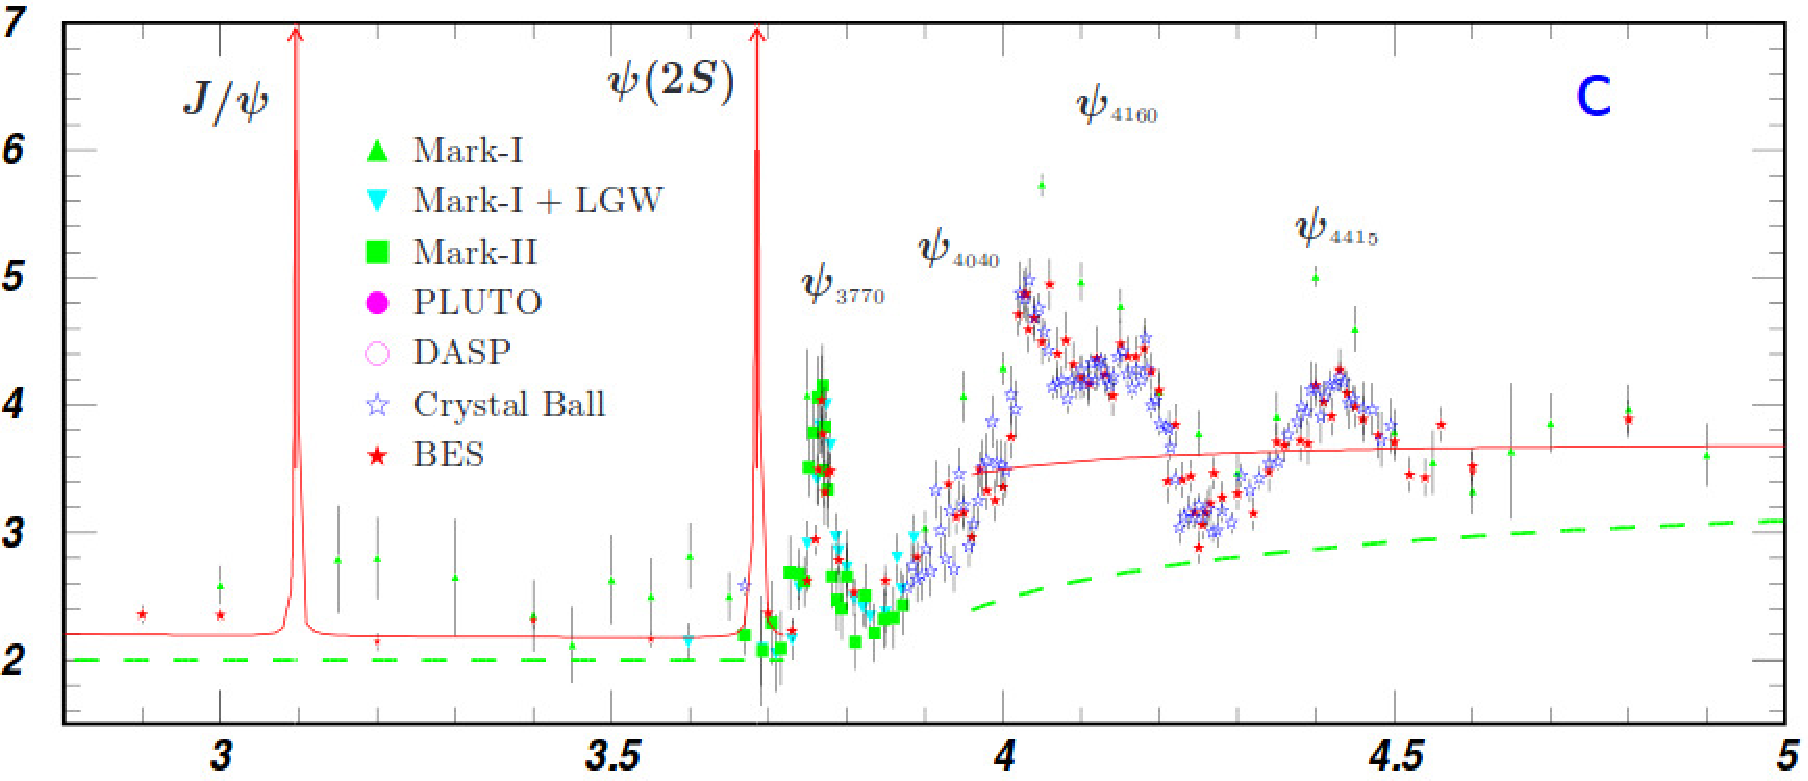
\includegraphics[scale=0.50]{figures/images/R_scan.pdf}
\caption{Measurements of $R = \sigma(\ee \rightarrow \text{hadrons}) / \sigma(\ee \rightarrow \mumu)$.}
\label{fig:R_scan}
\end{figure}

Many of the lower mass resonances are predictable within the context of the quark model.
However, there are a number of states which have been predicted, but not yet discovered.
There are also states which were discovered experimentally without any corresponding predictions.
A variety of these particles are shown in \Cref{fig:charmonia}.

\begin{figure}[H]
\centering
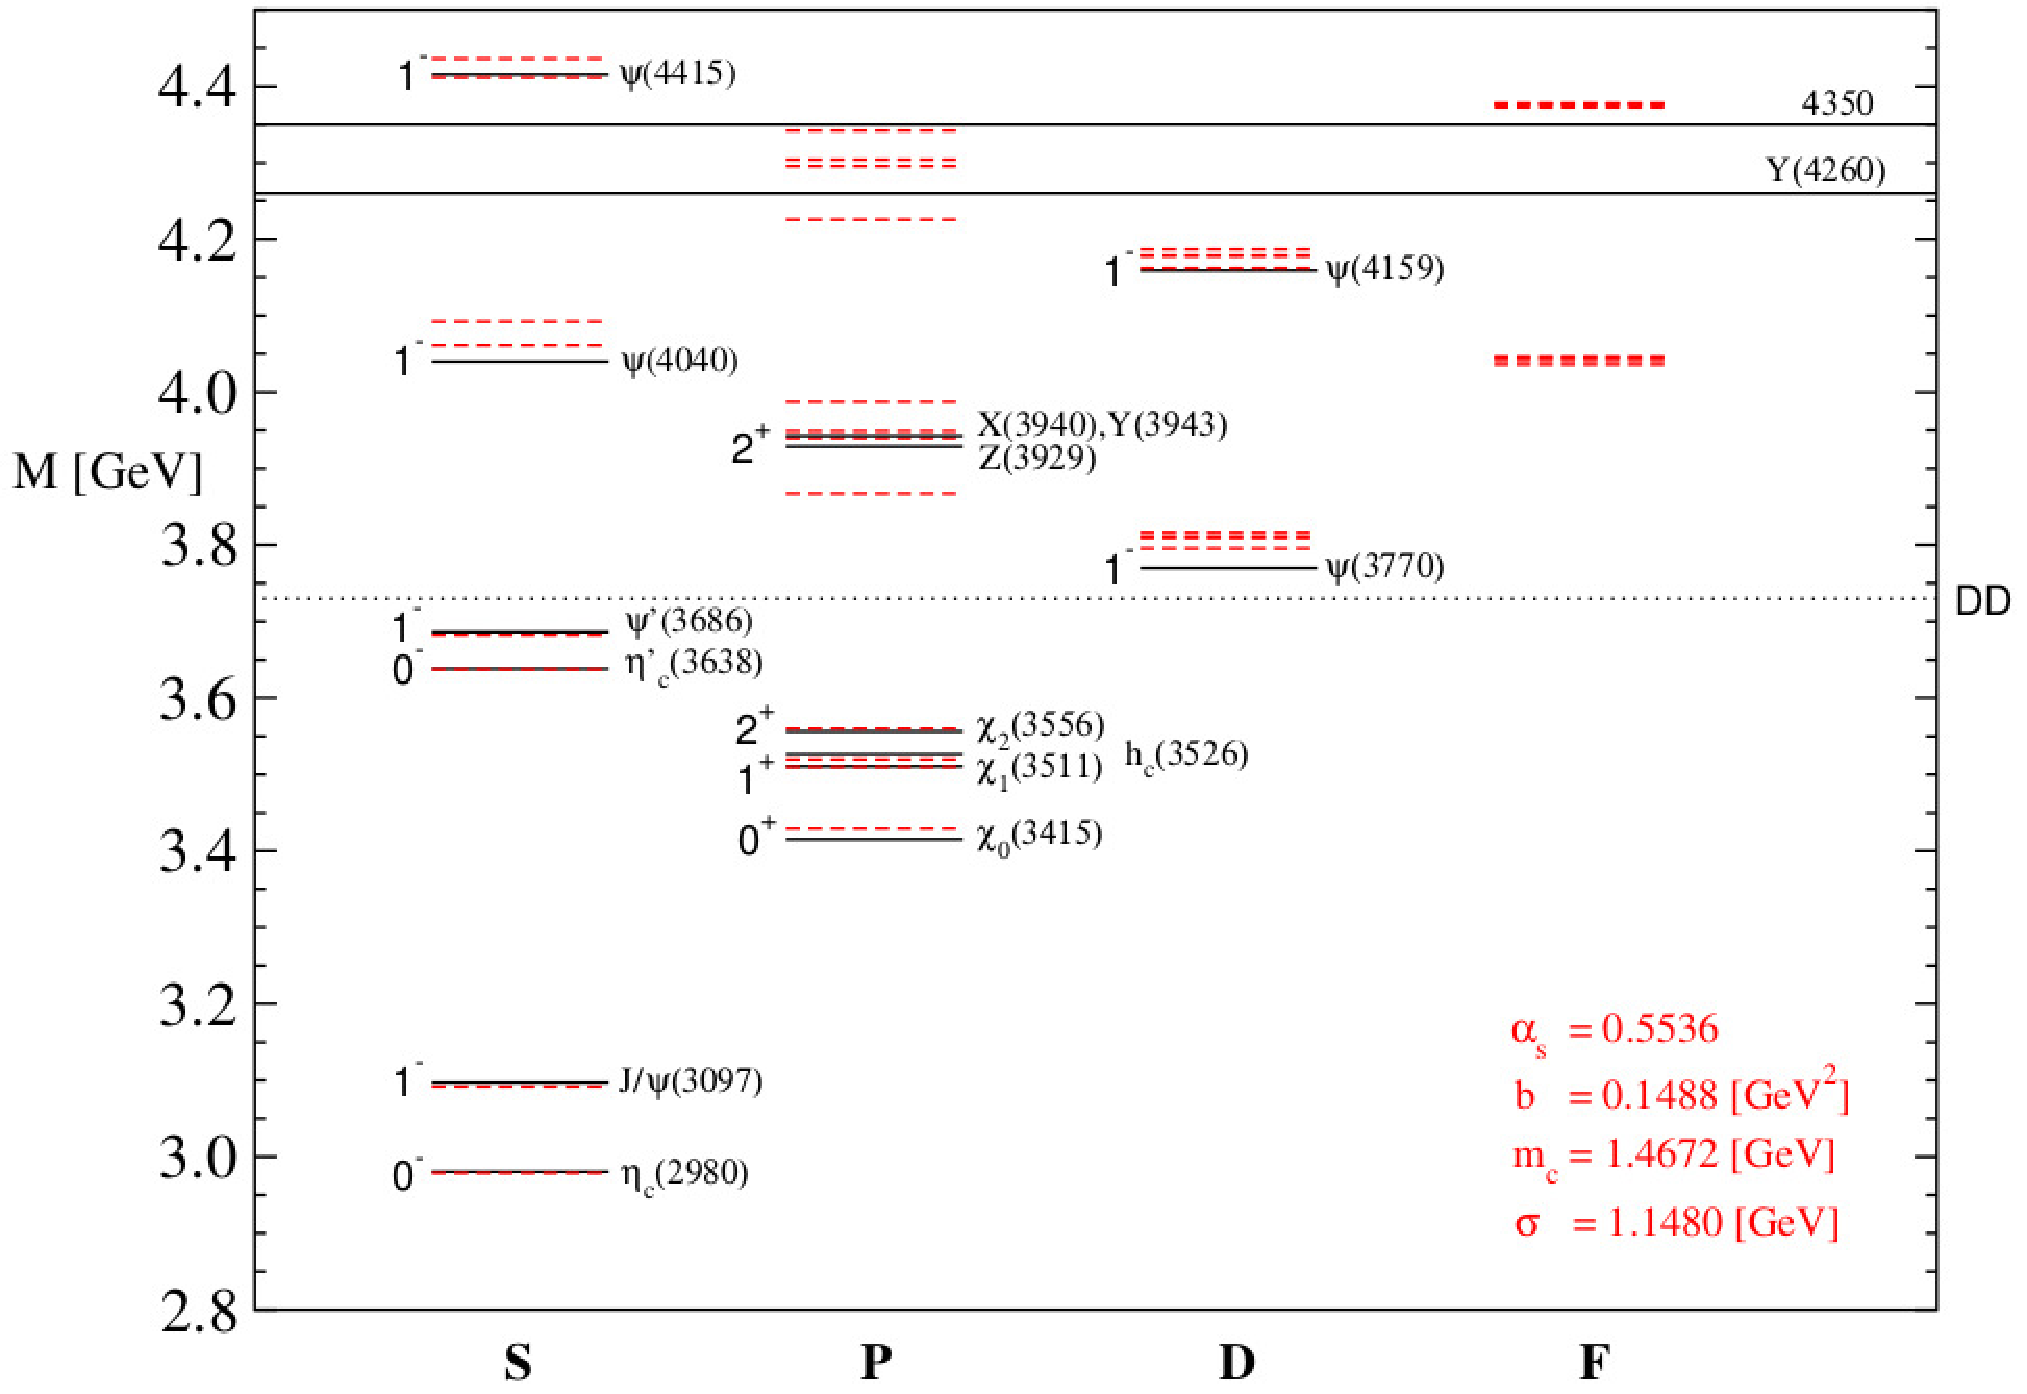
\includegraphics[scale=0.40]{figures/images/charmonia.pdf}
\caption{Measured and predicted charmonium resonances.}
{Solid black lines represent measurements while the dashed red lines are predictions.}
\label{fig:charmonia}
\end{figure}

The resonances below the $\DDbar$ threshold, like the $\jpsi$ and the $\psip$, show solid agreement with their theoretical predictions.
However, many of the ones above, such as the $\psipp$, still show some disagreement.
This is likely due to the more complicated interactions introduced from $\DDbar$ decays.
Several experiments have attempted to measure the shape of the $\psipp$ based on different assumptions.
The most prominent of these is the assumption of interference.
This can have notable effects on the resultant parameters of the $\psipp$, such as the mass, shown in \Cref{tab:previous_results}.

\begin{table}[H]
\centering
\begin{tabular}{c l|c l}
\hline
\multicolumn{2}{c|}{$\Mpsipp$ [\si{\MeV}] (No Interference)} & \multicolumn{2}{c}{$\Mpsipp$ [\si{\MeV}] (With Interference)} \\ [1pt] 
\hline
BES-II \cite{ref:Ablikim:2007}   & 3772.0 $\pm$ 1.9           & BaBar \cite{ref:Aubert:2008b} & 3778.8 $\pm$ 1.9 $\pm$ 0.9 \\
Belle  \cite{ref:Brodzicka:2008} & 3776.0 $\pm$ 5.0 $\pm$ 4.0 & KEDR  \cite{ref:Anashin:2012} & $3779.2^{+1.8 \, +0.5 \, +0.3}_{-1.7 \, -0.7 \, -0.3}$ \\ 
BaBar  \cite{ref:Aubert:2008a}   & 3775.5 $\pm$ 2.4 $\pm$ 0.5 & & \\
\hline
\end{tabular}
\caption{Previous experimental results for the mass of the $\psipp$.}
{Where applicable, the first errors are statistical, the second are systematic, and the third are model-dependent.}
\label{tab:previous_results}
\end{table}

Both BaBar \cite{ref:Aubert:2008b} and KEDR \cite{ref:Anashin:2012} found it necessary to include interference effects for fitting the $\DDbar$ spectrum.
However, the statistics of the KEDR sample were insufficient to fully resolve the discrepancies seen with other experiments that ignored interference.
{\bf Using the larger data sample available at BESIII, we have precisely measured and analyzed the shape of the $\DDbar$ spectrum around the $\psipp$ resonance.}
We have also used this measurement to probe the branching fraction of $\nonDDbar$ decays in this region.


\section{Procedure}
\label{sec:procedure}

The basis of this measurement involves identifying $\DDbar$ pairs which have decayed from $\psipp$.
All data used in this analysis was collected from $\ee$ collisions analyzed by the BESIII detector.
As $\lel$ and $\alel$ are fundamental particles, the total energy of each is transferred in the collision.
Additionally, the ability to precisely tune these two beam energies allows for the targeted production of specific particles, such as the $\psipp$.
However, resonances like this will decay almost instantaneously.
For example, the $\psipp$ has an average lifetime of ${\sim}\SI{e-23}{\s}$.
Even if it were traveling at $c$, the farthest distance this could travel would be $(\SI{3e8}{m/s}) \times ({\sim}\SI{e-23}{\s}) \approx \SI{1}{\fm}$.
This distance, approximately the radius of a proton, is far too small to be resolved by our detectors.
Even the initial decay into $\DDbar$ pairs is too small to precisely measure, as their lifetime of \SI{~4e-13}{\s} corresponds to a maximum distance of ${\sim}\SI{1}{\mm}$ if it were traveling at $c$.
However, the limited available energy in these decays ($m_{\psipp} - 2 \times m_{D} \approx \SI{40}{\MeV})$ means the velocity is much, much slower.

% \tau = 1 / 25 [1/MeV] * (200 MeV / 1e-15 m) / (3e8 m / s) = 200 / (3 * 25) e-23 s ~ 10^-13 s

Instead, the reconstruction of candidate $D$ particles relies on measuring their decays into other known modes.
While there are dozens of possible decays modes, we focus on those which have high branching fractions, and are comprised of particles identifiable by the BESIII detector.
For our purposes, these are $\pipm, \Kpm, \piO,$ and $\Ks$.
Each of these particles leave `tracks' within the detector; charged particles travel along curved paths and interact electromagnetically with charged wires along their trajectory, while neutral particles travel along straight paths and deposit bursts of energy after contacting crystals located along the inner walls of the detector.
The various components of the BESIII detector analyze these tracks to determine the type of particle, as well as its momentum and energy.
By analyzing sets of particles corresponding to the chosen decay modes, we can reconstruct the combination most likely to have originated from a $D$ based on their total energy.


To determine the $\psipptoDD$ cross section, we need to count the number of $\DDbar$ pairs produced, as well as measure the integrated luminosity, at each energy point in our data sample.
This counting is done not only for the actual collision data collected, but also for computed generated Monte Carlo (MC) background samples.
Each of these backgrounds corresponds to a particular event type which may be mistaken as signal, such as $\ee \rightarrow \tautau$.
We subtract these misidentified contributions from the total amount found in data to determine the actual number of reconstructed $\DDbar$ events.
Also from MC, we calculate the efficiency of reconstructing $\DDbar$ decays based on our selection criteria.
By dividing the actual reconstructed events by this efficiency, we identify the true number of $\DDbar$ events produced.
Then, using the measured luminosity for each energy point, we determine the cross section as a function of center-of-mass energy.

% 
% While energy and momentum conservation remain fundamental laws of physics, accounting for the 
% 
% Also must correct for initial state radiation
% Accelerated particles (such as those traveling around a circular collider) radiate energy
% This energy reduces the total amount available in a collision
% Can lead to producing lower resonances (jpsi, psip) instead of targeted psipp
% Also decreases total energy available at each point, and must be accounted for
% Effect is very calculable, and included in cross section derivation


The specific details of this analysis start with background on relevant theoretical concepts.
Next, we list the specifications for the collider and detector which collected the data used for these measurements along with their related analysis software and reconstruction methods. 
From here, we further describe the procedure for determining the $\psipptoDD$ cross section and show the results with systematic uncertainties.
Finally, we examine the current progress of measuring the $\nonDDbar$ branching fraction.



% Main Chapters
\chapter{Theoretical Background}
\label{ch:theory}

\section{Standard Model}
\label{sec:standard_model}

Developed throughout the 1960s and 1970s, the Standard Model provides the most complete description of observable matter in the universe to date.
It is a classification of all confirmed subatomic particles currently known, and predicts the most accurate results of any scientific theory ever measured.
Each of the electromagnetic, weak, and strong fundamental forces are well described by this formulation.
These three are described by an $\SUthree \times \SUtwo \times \Uone$ group, where the $\SUthree$ corresponds to the strong force, the $\SUtwo$ corresponds to the weak force, and the $\Uone$ corresponds to the electromagnetic force.
The remaining fundamental force, gravity, is not included in the Standard Model.
It is negligible on the scale of the masses of fundamental particles, and will be ignored in the discussions that follow.


\subsection{Electromagnetic Force}
\label{ssec:electromagnetic}

The electromagnetic force is responsible for the forces between objects with electric charge, most notably binding together electrons and protons to form atoms and the structures they comprise.
The theory of electromagnetic interactions is known as Quantum Electrodynamics (QED).
Within this theory, the mediator of this force is the photon, a massless vector boson.
As there is only a single mediator, and a single conserved quantity (electric charge), the formulation of QED is relatively simple compared to the other forces.
Still, the predictions it makes show astounding consistency with experiment, such as correctly calculating the anomalous magnetic dipole moment of the electron to more than 10 significant figures.
Much of this success is due to QED being calculable through perturbation theory, where corrections are applied in terms of higher order factors of the coupling constant, $\alphaQED$.
This is possible due to its relatively small value ($\alphaQED \approx 1/137$), as the terms are convergent below very high orders of $\alphaQED$. 

\subsection{Weak Force}
\label{ssec:weak}

The weak force is responsible for radioactive decay and other subatomic phenomena.
This is distinct from the electromagnetic and strong interactions, where the constituent particles cannot change their types (or flavors).
The mediators of this force are the $\W$ and $\Z$, which are massive vector bosons.
Not only are each of their masses non-zero, they are extremely heavy particles at \SIlist{80.4;90.2}{\GeV}, respectively \cite{ref:Olive:2014}.
These large masses not only limit the interaction distance of the weak force, but also minimize the interaction strength (which is inversely proportion to mass).
Furthermore, the large $\W$ and $\Z$ masses also lead to much slower interaction times, further reducing the effects of the weak force in comparison to the strong and electromagnetic forces.


In addition to transforming particle flavor, the weak force is also unique in its violation of various symmetries.
The first discovery of symmetry violation came in 1957, when Wu and others \cite{ref:Wu:1957} discovered the weak force did not behave identically under parity ($\sP$) transformations (i.e., mirror reflection).
To account for this, a new theory conserving a compound symmetry was proposed.
This combined charge conjugation ($\sC$), the swapping of particles with their antiparticles, with parity to form $\sCP$ parity.
However, in 1964, evidence of $\sCP$ violation was also discovered by Cronin and Fitch \cite{ref:Christenson:1964}.
The resolution to this symmetry conservation involves yet a third symmetry, time reversal ($\sT$), in which time is replaced with its negative ($t \rightarrow -t$).
While the weak force violates these symmetries individually, the application of all three ($\sCPT$) is conserved across all known processes, and is known as the $\sCPT$ Theorem.


At higher energy scales, the electromagnetic and weak forces unify into the electroweak force.
In this theory, there are initially four massless gauge bosons mediating the interactions.
As a result of the Higgs mechanism, the initial gauge symmetry is broken at lower energies, and three of these bosons acquire a mass.
These three bosons are the $\W^\pm$ and $\Z$, while the remaining massless boson is the $\photon$.
The energies scales required for this unification were only present in the early universe.
Before this, it is also believed there was an epoch of even higher energy, in which the electroweak force merged with the strong force.


\subsection{Strong Force}
\label{ssec:strong}

The strong force is responsible for binding together particles known as hadrons.
The theory of strong interactions is known as Quantum Chromodynamics (QCD).
Like the electromagnetic force, the mediator of the strong force is also a massless vector boson, the gluon.
However, while massless particles typically correspond to an infinite interaction range, the strong potential becomes very large at higher separations.
This prevents particles which interact through the strong force, known as quarks (see \Cref{sssec:fermions}), from existing as isolated entities in a process known as confinement.
The typical interaction range is on the order of the proton radius, around \SI{e-15}{\m}.
QCD calculations face serious challenges, however, as the coupling constant is not small ($\alphaQCD \gtrsim 1$).
This excludes the use of perturbation theory for most cases, as the higher order terms do not converge.


Strong interactions are associated with a corresponding conserved quantity known as the color charge. 
Despite its name, however, the term 'color' has no association with light, which is a purely electromagnetic phenomena.
There are three colors associated with this charge, red ($\cRed$), green ($\cGreen$), and blue ($\cBlue$).
For anti-particles, there are oppositely charged values ($\acRed, \acGreen,$ and $\acBlue$).
In order for hadrons to be formed, the total color values of the constituents must be colorless.
This means the total sum must involve all three colors ($\cRed \cGreen \cBlue$ or $\acRed \acGreen \acBlue$) or pairs of opposite colors ($\cRed \acRed, \cGreen \acGreen, $ or $\cBlue \acBlue$).
However, these individual colors are not observable in nature.
Because particles with different color values are distinct, this effectively triples the number of possible particle combinations, due to combinatorics.


Unlike the photon, which does not carry an electric charge, gluons do possess a color charge.
There are eight possible color combinations which a gluon may possess, which are typically expressed using the Gell-Mann representation of $\SUthree$.
With this basis, each gluon is linearly independent, and no combination of gluons can be used to form a color singlet state.
This non-zero charge of the force carrier makes QCD significantly more complex than QED.
In fact, carrying color charge means gluons can also interact with each other directly, leading to certain theoretical states such as glueballs. 


\subsection{Elementary Particles}
\label{ssec:elementary_particles}

There are two primary groups contained in the Standard Model, fermions and bosons. 
This division is based on the Spin Statistics theorem, where fermions (bosons) have half-integer (integer) spins.
As described by the Pauli Exclusion principle, nature restricts fermions from occupying the same quantum state.
Bosons, however, do not have this restriction, and can have any number occupying the same state.

\begin{figure}[H]
\centering
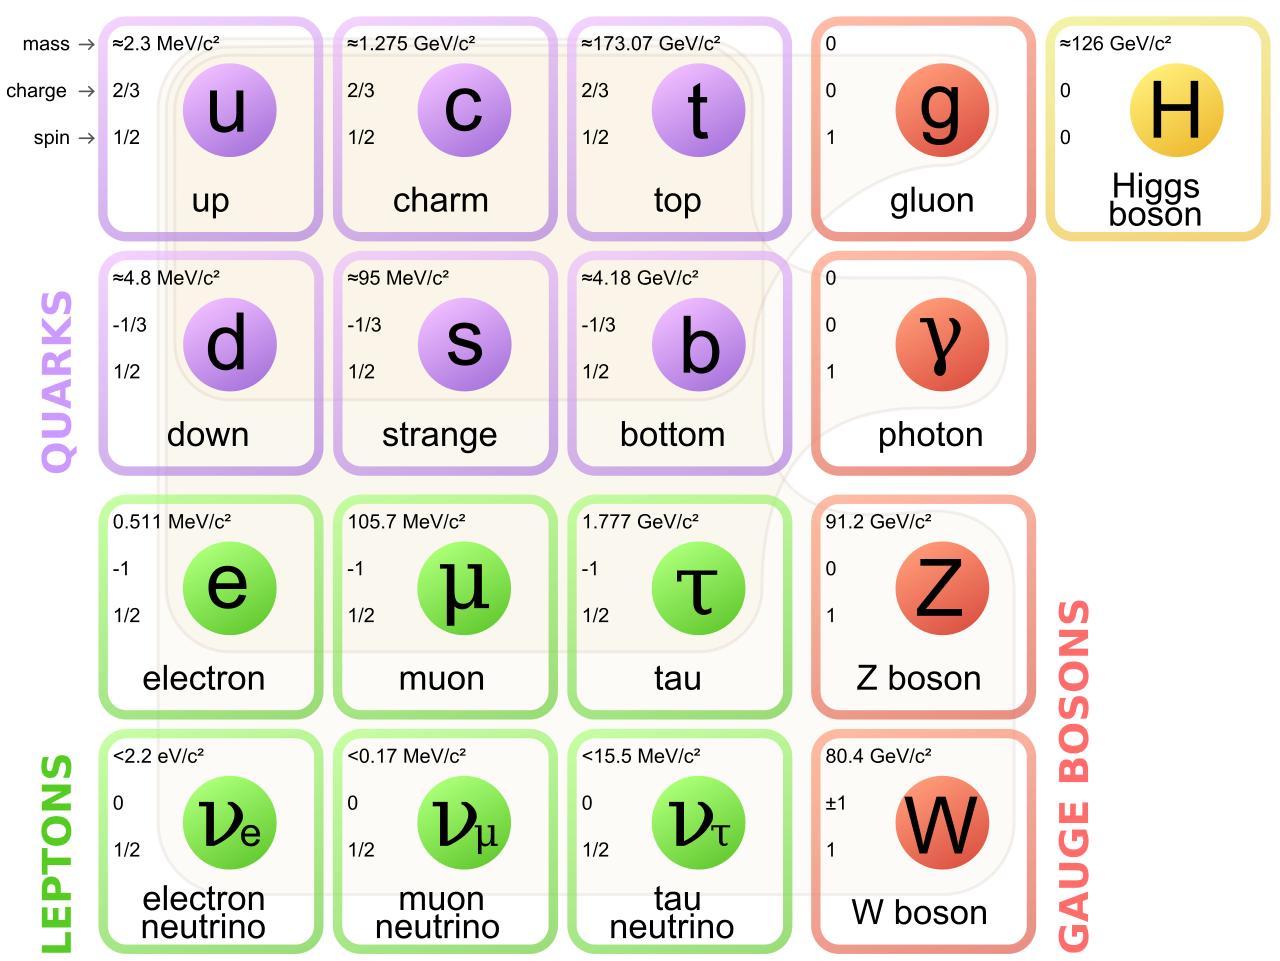
\includegraphics[scale=0.30]{figures/images/standard_model.png}
\caption{The standard model of particle physics.}
{It is comprised of two main groups: fermions, which includes the quarks and leptons, and bosons, which includes the gauge bosons and the Higgs boson. Image reproduced courtesy of \cite{ref:Wikimedia:2006}. }
\label{fig:standard_model}
\end{figure}


\subsubsection{Fermions}
\label{sssec:fermions}

The fermions are divided by their interaction types into two major groups, quarks ($\quark$) and leptons ($\lepton$).
Each of these groups contains six particles with their corresponding antiparticles.
These can be grouped into three generations, which aligns particles with the same electric charges, but greatly differing masses.  
As an example, the up ($\qup$), charm ($\qcharm$), and top ($\qtop$) quarks all have an electric charge of +2/3 (in terms of the electron charge, $e$), but $\qtop$ is approximately five orders of magnitude more massive than $\qup$.
For the quarks and fermions in \Cref{fig:standard_model}, rows indicate particles with the same electric charge, while columns represent each generation of particles.


Although all fermions interact both electromagnetically and weakly, only the quarks interact strongly.
Because of confinement, quarks cannot exist as isolated particles, and are only found in nature as groups of particles called hadrons.
The most common types of hadrons exist as quark-antiquark pairs, known as mesons, or as groups of three quarks (or antiquarks), known as baryons.
There are, however, indications of more exotic combinations of quarks, such as tetra- ($\quark\quark\aquark\aquark$) or penta-quark ($\quark\quark\quark\quark\aquark$) states seen by recent experiments \cite{ref:Ablikim:2013,ref:Liu:2013,ref:Aaij:2015}.


While the negatively charged quarks ($\qdown, \qstrange$, and $\qbottom$) are labeled as definite states, the quarks are actually mixed states.
Through weak interactions, each of these quarks can transform into other quarks.
The probabilities for these transformations are expressed by the Cabibbo-Kobayashi-Maskawa (CKM) Matrix \cite{ref:Kobayashi:1973}, shown in \Cref{fig:ckm_matrix}.
From the experimentally measured values \cite{ref:Olive:2014}, is it evident the matrix is nearly diagonal.
It is also clear that correlations are strongest within each generation, as the off-diagonal terms are generally smaller than the diagonal ones.
Additionally, though the convention splits the negatively charged quarks into mixed states (leaving the positively charged quarks fixed), this choice has no physical basis.
The reverse choice of having mixed positively charged quarks is equivalent.

\begin{figure}[H]
\centering
$
\begin{bmatrix}
   |V_{ud}| & |V_{us}| & |V_{ub}| \\
   |V_{cd}| & |V_{cs}| & |V_{cb}| \\
   |V_{td}| & |V_{ts}| & |V_{tb}| \\
\end{bmatrix}
=
\begin{bmatrix}
    0.97427 \pm 0.00014 & 0.22536 \pm 0.00061 & 0.00355 \pm 0.00015 \\
    0.22522 \pm 0.00061 & 0.97343 \pm 0.00015 & 0.0414  \pm 0.0012  \\
    0.00886^{+0.00033}_{-0.00032} & 0.0405^{+0.0011}_{-0.0012} & 0.99914 \pm 0.00005 \\
\end{bmatrix}
$
\caption{The Cabibbo-Kobayashi-Maskawa (CKM) Matrix.}
\label{fig:ckm_matrix}
\end{figure}

The values of the CKM matrix are typically parameterized using three Euler angles ($\theta_{12}, \theta_{23}, \theta_{13}$) and a $\sCP$-violating phase parameter ($\delta_{13}$), where the indices represent the three generations of quarks.
This formulation allows the matrix to be cast in the ``standard'' parametrization, shown in \Cref{fig:ckm_standard}.
The form with three separated matrices clearly shows the connections between each generation of quarks.
Namely, the third shows the original formulation in terms of a single rotation, the Cabbibo angle ($\theta_{12}$).
This theory is known as the Glashow-Iliopoulos-Maiani (GIM) mechanism [\cite{ref:Glashow:1970} and was used to explain the suppression of flavor-changing neutral currents (FCNC) before the discovery of the charm quark.
% Current measurements for the standard parameters are $\theta_{12} = \ang{13.04 \pm 0.05}, \; \theta_{13} = \ang{0.201 \pm 0.011}, \; \theta_{23} = \ang{2.38 \pm 0.06}$ and $\delta_{13} = \SI{1.20 \pm 0.08}{\rad}$.

\begin{figure}[H]
\centering
$
    \begin{bmatrix}
        1 &  0      & 0      \\
        0 &  c_{23} & s_{23} \\
        0 & -s_{23} & c_{23} \\
    \end{bmatrix}
    \begin{bmatrix}
         c_{13}                  & 0 & s_{13} e^{-i\delta_{13}}  \\
         0                       & 1 & 0                         \\
        -s_{13} e^{i\delta_{13}} & 0 & c_{13}                    \\
    \end{bmatrix}
    \begin{bmatrix}
         c_{12} & s_{12} & 0 \\
        -s_{12} & c_{12} & 0 \\
         0      & 0      & 1 \\
    \end{bmatrix}
\linebreak
=
    \begin{bmatrix}
          c_{12} c_{13} 
       &  s_{12} c_{13}
       &  s_{13} e^{-i\delta_{13}} \\
         -s_{12} c_{23} - c_{12} s_{23} s_{13} e^{i\delta_{13}}
       &  c_{12} c_{23} - s_{12} s_{23} s_{13} e^{i\delta_{13}}
       &  s_{23} c_{13} \\
          s_{12} s_{23} - c_{12} c_{23} s_{13} e^{i\delta_{13}}
       & -c_{12} s_{23} - s_{12} c_{23} s_{13} e^{i\delta_{13}}
       &  c_{23} c_{13} \\
    \end{bmatrix}
$
\caption{The standard form of the Cabibbo-Kobayashi-Maskawa (CKM) Matrix.}
    {The parameterization is in terms of three angles ($\theta_{12}, \theta_{23}, \theta_{13}$) and a phase angle ($\delta_{13}$). Here, $c_{ij} = \cos\theta_{ij}$ and $s_{ij} = \sin\theta_{ij}$.} 
\label{fig:ckm_standard}
\end{figure}

The leptons are also organized into generations consisting of particles with two distinct charges.
The electron ($\lel$), muon ($\lmu$), and tau ($\ltau$) are all negatively charged particles.
There is also a neutral particle, a neutrino ($\neutrino$), corresponding to each of the charged leptons ($\vel, \vmu, \vtau$).
These are very small mass ($< \SI{1}{\eV}$) particles with extremely low interactions.
With the exception of mass, the interaction properties of each flavor is very similar.
However, the three flavors themselves are treated as separate conserved quantities.


The Standard Model assumes neutrinos to be massless particles.
However, this was violated by the discovery of neutrino oscillations, where transformations occur between neutrino flavor states due to differences in their masses.
As with the quarks, the flavor states, $\vel, \vmu$, and $\vtau$, are not the states observed in nature.
Rather, the states with definite mass, labeled $\nu_1, \nu_2,$ and $\nu_3$, are linear combinations of the three flavor states.
This can be expressed in a rotation of bases called the Pontecorvo-Maki-Nakagawa-Sakata (PMNS) matrix \cite{ref:Pontecorvo:1957,ref:Maki:1962}.
Its formulation is analogous to the CKM Matrix for quarks. 


\subsubsection{Bosons}
\label{sssec:bosons}

For each of the three forces included in the Standard Model, there are accompanying gauge bosons.  
These are the photon ($\photon$) for electromagnetic force, the $\W^\pm$ and $\Z$ for the weak force, and the gluon ($\gluon$) for the strong force.
Each of the gauge bosons is a spin-1 vector boson, which means there are three available polarization states (-1, 0, +1).  
However, since the photon and gluon are both massive, gauge invariance requires these to have transverse polarizations.
This means the spin-0 state is eliminated, and there are only two polarization states for each.
There is also the Higgs boson ($\Higgs$), which unifies the electromagnetic and weak forces, and whose interactions with other particles is responsible for their mass.
This is the only known fundamental spin-0 particle, which means it has only one polarization state.


Even with the amazing success of the Standard Model, the theory is not complete.  
Along with neutrino oscillations, other effects, such as dark matter and dark energy, remain major obstacles to constructing a unified theory.
Such a theory must also include gravity, but there remain significant difficulties in explaining its effects through a quantum field theory.
There also remains no conclusive explanation for various constants, such as the masses of each fundamental particle.
Still, the Standard Model remains the most precise description of the universe to date, and continues to provide the basis for much current and future experimental and theoretical work.


\section{Charmonium}

The majority of this analysis focuses on a specific group of particles known as Charmonium.
These particles are resonances formed by a $\qcharm \aqcharm$ pair, and can be treated analogously to the hydrogen atom.
Namely, there is a spectrum of various excited states in the Charmonium region, just as the spectrum of states associated with the emission lines of hydrogen.
The first three charmonium states to be discovered were the $\jpsi, \psi'$, and $\psi''$.
The $'$ and $''$ marks indicate these are the first and second excited states of the $\jpsi$, respectively.
More commonly, the $\psi'$ is denoted $\apsip$ and the $\psi''$ is denoted $\psipp$.
The numbers in parentheses represent the mass of the particle in $\si{\MeV}$.


An alternative labeling scheme for these states uses the quantum numbers for each particle.
This is written in the form $N^{2s+1}L_J$, where $N$ refers to the principal quantum number, $s$ refers to the total spin angular momentum of the particle, $L$ refers to the orbital angular momentum, and $J$ refers to the total angular momentum.
Here, the values of $L$ are in spectroscopic notation, where $L = 1, 2, 3, 4 \ldots$ is denoted $S, P, D, F \ldots$, and higher values follow alphabetically (excluding $J$).
As each of these states is comprised of two spin-$\half$ particles, the value of $s$ in this case can only be 0 (opposite) or 1 (aligned).
With this, the $\jpsi, \apsip$, and $\psipp$ can be denoted $1^3 S_1, \, 2^3 S_1$, and $1^3 D_1$.
The values of $n$ and $L$ are used for the alternate notation of $\psip$ representing $\apsip$.
However, the notation of $\psi(1D)$ is not often used for $\psipp$.
This is due to evidence of mixing in $\psipp$ between the $2^3 S_1$ and $1^3 D_1$ states that suggests more complicated underlying interactions \cite{ref:Rosner:2001,ref:Rosner:2004}.


In fact, while the comparisons from this model work well for states less massive than the $\psipp$, the predictions made above this often break down.
This is likely based on the energy required to produce open-charm $D$ mesons, such as $\Dp (\qcharm\aqup)$ and $\DO (\qcharm\aqdown)$.
The $\DDbar$ threshold (twice the mass of the $\DO$) is just above the $\psip$ mass, and just slightly below the $\psipp$ mass.
Therefore, the decay products of the two particles are drastically different, even while the available phase space is similar.
Example Feynman diagrams for these two particles can be seen in \Cref{fig:OZI_psip,fig:OZI_psipp}.


\begin{figure}[H]
\centering
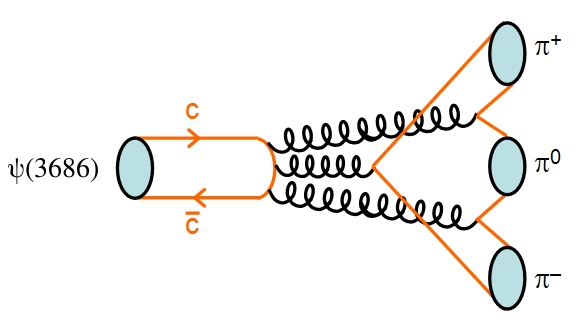
\includegraphics[scale=0.50]{figures/images/OZI_psip.png}
\caption{An example Feynman diagram for the decay of $\apsip$.}
{Without sufficient energy to produce $D$ mesons, the decays of $\apsip$ must be mediated by three hard gluons and are suppressed, as described by the OZI rule.}
\label{fig:OZI_psip}
\end{figure}

\begin{figure}[H]
\centering
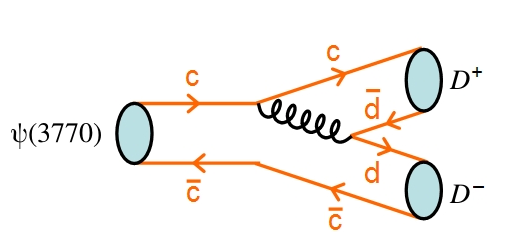
\includegraphics[scale=0.50]{figures/images/OZI_psipp.png}
\caption{An example Feynman diagram for the decay of $\psipp$.}
{With sufficient energy to produce $D$ mesons, the open-charm decays of $\psipp$ are allowed to proceed, greatly increasing the total decay width.}
\label{fig:OZI_psipp}
\end{figure}


The difference is also clearly seen in the total decay widths, where the most recent experimental averages \cite{ref:Olive:2014} are $\Gpsip = \SI{286}{\keV}$ and $\Gpsipp = \SI{27.5}{\MeV}$.
An explanation for this discrepancy was proposed independently in the 1960s by Okubo \cite{ref:Okubo:1963}, Zweig \cite{ref:Zweig:1964}, and Iizuka \cite{ref:Iizuka:1966}, and is named the OZI rule.
This states that any Feynman Diagram where the initial and final particles are separated at some point by only gluons represents a suppressed decay.
Such behavior requires that the momentum transfer from the initial particles must occur entirely through these gluons.
Because of the decreasing strength of the strong interaction with higher momentum transfer, the rate of these decays is thereby inhibited.
This is further compounded by the need for three gluons in such an interaction, as one gluon could not conserve color charge, and two could not converse $\sC$-parity.
Once above the $\DDbar$ threshold, the allowed open-charm decays dominate, and the total width is greatly increased.
This dominance points to a high branching fraction expected for decays of the type $\psipptoDD$.


\chapter{Detector and Related Systems}
\label{ch_detector}

\section{BEPCII Accelerator}

\section{BESIII Detector}

\subsection{Multi-Layer Drift Chamber}

\subsection{Time-of-Flight System}

\subsection{Electromagnetic Calorimeter}

\subsection{Muon Identifier}

\section{Triggering Systems}
\chapter{Analysis Software}
\label{ch:software}

\section{BESIII Offline Software System}

Reconstructing and processing event data gathered by the BESIII detector is done using the BESIII Offline Software System (BOSS) \cite{ref:Li:2006}.
This is an analysis software distribution written using the C++ language and running primarily on the Scientific Linux CERN operating system \cite{ref:SLC5}.
There are five main parts to BOSS: framework, simulation, reconstruction, calibration, and analysis.


\subsection{Framework}

The framework is built on the Gaudi software architecture \cite{ref:Barrand:2001}, which provides a standard interface and utilities for things such as event simulation, data processing, and physics analysis.
The software is managed using the Configuration Management Tool \cite{ref:Arnault:2000}, which provides a method for creating packages, handling package dependencies, and producing executables from source code.
There are three main filetypes for data stored by the framework: raw data ($\texttt{.raw}$), reconstructed data ($\texttt{.rec}$), and Data-Summary-Tape ($\texttt{.dst}$).
The latter two of these file types are derived from the ROOT \cite{ref:ROOT} format ($\texttt{.root}$) for easy management and usage in various analyses.


\subsection{Simulation}

There are four main parts to the simulation process: event generation, detector description, particle tracking, and detector response.
Event generation is primarily handled by the Monte Carlo (MC) generators KKMC, BesEvtGen, and Babayaga, which are described below.
To model its geometry and materials, a unique description of the detector has been created using a format based on XML.
This allows both simulation and reconstruction packages to appropriately model the behavior of events within the specific environment of BESIII.
For particle tracking, interactions with detector materials are handled by GEANT4 \cite{ref:Agostinelli:2003}.
Lastly, detector responses are modeled by the so-called `digitization code'.
This takes into account each detector component, as well as readout electronics, and realistic situations such as noise or dead channels.
There is also a simulation of the triggering system implemented.


\subsubsection{KKMC}

Originally developed for the LEP and SLC colliders, KKMC \cite{ref:Jadach:2000} is a generator used to model electroweak interactions.
Namely, the processes generated are of the form $\ee \rightarrow \ffbar + (n)\photon$, where $\fermion = \{ \mu, \tau, \qup, \qdown, \qstrange, \qcharm, \qbottom \}$, and $(n)\photon$ represents any number of additional photons.
These are modeled taking into account second-order sub-leading corrections, as well as initial-state radiation (ISR), and interference between initial- and final-state radiation (FSR).
The effects of beam energy spread, typically on the order of \SI{1}{\MeV} near the $\psipp$, can also be included.


After generation, the $\ffbar$ pair is decayed by models depending on the fermions involved.
The TAUOLA library \cite{ref:Jadach:1993} is used to decay $\tautau$ pairs, and takes into account spin-polarization effects.
The PYTHIA model \cite{ref:PYTHIA} is used to hadronize final-state $\qqbar$ continuum production using the parton shower model.
For resonances like the $\psipp$, the only action performed by KKMC is the generation of ISR.
After this, the virtual photon produced is handed off to BesEvtGen.


\subsubsection{BesEvtGen}

Originally developed for the CLEO and BaBar collaborations, EvtGen \cite{ref:Lange:2001} is another widely used generator.
It is the basis for BesEvtGen \cite{ref:Ping:2008}, which incorporates many different decay models into a single utility.
Over 30 exclusive decay models are available in BesEvtGen, as well as the capability to incorporate user-created models.


The simulation process occurs sequentially using dynamic information from decay amplitude probabilities and forward/backward spin-density matrices.
From this, final state radiation is handled by the PHOTOS model \cite{ref:Barberio:1991}.
To generate unknown decays of charmonium resonances, the LundCharm model \cite{ref:Chen:2000} is used, while other unknown hadronic decays are handled by PYTHIA.
For radiative processes, such as radiative return to $\jpsi$ or $\psip$, the VECTORISR model \cite{ref:Bonneau:1971} is used.
This occurs when one particle in the initial $\ee$ pair radiates a photon of high enough energy that only lower mass resonances can be produced from the reduced center-of-mass energy.
When the radiation is less energetic, the $\psipp$ resonance is directly produced through the combination of KKMC and BesEvtGen.


\subsubsection{Babayaga}

Production of QED processes is done using the Babayaga generator \cite{ref:Carloni:2004}.
This includes $\ee \rightarrow \{\ee, \mumu, \yy\}$.
The results are very accurate, with an estimated theoretical uncertainty of \SI{0.1}{\%}.
It also matches exact next-to-leading-order corrections from the parton shower algorithm.
The high precision is important for determination of the efficiencies and acceptances required to precisely measure the integrated luminosity.

\subsection{Reconstruction}

Reconstruction primarily involves information about specific types of particles from each of the four main detector subsystems.
These sources of information are as follows:
\begin{itemize}
    \item a charged track finding algorithm and a Kalman-filter-based track-fitter
    \item a particle identifying algorithm based on $\tdEdx$ and time-of-flight measurements
    \item a shower- and cluster-finding algorithm for EMC energy and position 
    \item a muon track finding algorithm
\end{itemize}
Further descriptions of each of these processes can be found in Sec. \ref{sec:detector_simulation}.
Additionally, algorithms for determining the corresponding beam bunch crossing, as well as for secondary vertex and track refitting, are also utilized.


\subsection{Calibration}

To maintain consistent production and analysis of datasets, a centralized source of run-dependent information is maintained by BOSS.
This includes algorithms which determine the calibration constants for each sub-detector, as well as a centralized database to store the results.
Each of the calibration outputs are stored in a ROOT file along with other details such as the beam energy, luminosity, magnetic field information, trigger conditions, and hardware/software versions.
While all of this information is stored by a central MySQL \cite{ref:MySQL} server at IHEP, other institutions in BESIII regularly synchronize with this server to create mirrored copies of these databases.



\section{Detector Simulation}
\label{sec:detector_simulation}

The following sections detail the simulation, calibration, and reconstruction processes for each detector subsystem.
Each of these relies on a geometry description created using GEANT4.


\subsection{Multi-Layer Drift Chamber}

Simulating events in the MDC accounts for axial layers, stereo layers, and endplates.
The simulation also relies on the calibration parameters to determine things such as wire efficiency and resolution as a function of drift distance for each wire, noise in each layer, and possible misalignment.


Calibration of the MDC relies on $\jpsi \rightarrow \mumu$ for both position and $\tdEdx$.
Using $\jpsi$ events allows for quickly obtaining sufficient statistics due to the very large production cross section at that peak.
The information determined includes constants such as $x-t$ relations, timing, alignment, and absolute wire efficiency.
These values are stored in the database for each run.
Special-purpose runs with the magnetic field turned off allow precise determination of wire positions.


Reconstructing MDC events starts by finding axial track segments using raw hits.
These are found by searching for matches to pre-determined patterns.
Next, these segments are fitted to circular tracks using the least-squares method.
Stereo segments are then added using an iterative helix fit.
Lastly, additional hits which were possibly missed from the initial reconstruction are added to the track using a Kalman-filter process.
This process determines the track parameters for multiple particle hypotheses.
The reconstruction is remarkably efficient, with over \SI{98}{\%} of tracks with $p_T > \SI{150}{\MeV}$ being reconstructed, even amidst high backgrounds.
From this, the charge, momentum, and trajectory can be determined for each track.


In addition to tracking, the MDC also measures the ionization energy deposited per unit length, $\tdEdx$, for each particle.
The energy deposition of each track as it passes through the chamber is compared to expectations to determine a probability for each particle hypothesis.
Corrections applied account for things such as multiple scatterings, magnetic deflection, and ionization.
This likelihood from $\tdEdx$ is combined with information from the ToF to determine the type of particle that best matches the track properties.


\subsection{Time-of-Flight System}

Simulating events in the ToF accounts for the scintillator, wrapping materials, and photomultiplier tubes (PMTs).
The process converts the energy deposited in the scintillator into photons, then propagates the shape of a photon pulse (rather than individual photons) to the PMTs in order to generate an electronic signal.
A discriminator is applied to each pulse to determine the analog-to-digital conversion (ADC) and time-to-digital conversion (TDC) outputs.
The algorithm was designed and tested with dedicated test beam data, however, each new data set requires updated tuning.
A full simulation tracing each optical photon is also available for detailed study of the timing measurements.


Calibration of the ToF also uses $\jpsi$ decays to dileptons for both timing and energy measurements.
The information determined includes effective velocity, attenuation length, and muon energy loss.
The status and performance of the ToF are regularly monitored by a laser-fiberoptics pulsing system.


Reconstructing ToF events starts by using tracks with trajectories extrapolated from the MDC.
Each track is matched with a particular ToF module; either the two layers of the barrel, or the single-layer endcap.
The travel time for each hypothesis is then calculated using weighted-average times from PMTs at both ends of the scintillator.
Corrections are also applied to account for aspects like the effective light velocity in the scintillator and the light attenuation length.
Measurements of deposited energy are obtained for both charged and neutral particles, and are added to the EMC to improve the shower energy resolution.


\subsection{Electromagnetic Calorimeter}

Simulating events in the EMC accounts for the crystals, casing, silicon photodiodes, preamplifier boxes, cables, and the support system.
For each of the crystals and photodiodes, hit information is recorded, and the deposited energy is summed.
From this, photon statistics are computed, and the resulting photodiode response is converted into electronic signals.
To obtain the waveform in the time domain, an inverse Laplace transform is applied.
Then, a sampling and peak searching process is simulated to yield energy and time information.
For each bin, Gaussian-type electronic noise is added, and the background is produced by summing over the waveforms.


Calibration of the EMC uses Bhabha electrons with $E > \SI{1.55}{\GeV}$ for the high energy response, and $\piO \rightarrow \yy$ decays for the low energy response.
The responses for individual crystals must be analyzed separately, due to their potential intrinsic variations.
As a result, they are monitored frequently by a LED light pulser, and periodically recalibrated.
Corrections due to temperature variations are also applied.


Reconstructing EMC events starts by converting the ADC value of each crystal into energy based on the calibration constants.
After this, clusters in both the barrel and endcaps are formed by analyzing local maximum energy deposits, called seeds.
A clustering algorithm then aggregates hits around these seeds and sums the values for a particular shower.
The position of each shower is then calculated using the energy-weighted first moment.
If multiple seeds are found in one cluster, a splitting algorithm is invoked to split the cluster into multiple showers.
Additionally, matching energy deposits from the ToF are also added back into the total shower energy.
This improves the energy resolution, particularly for low energy photons.


\subsection{Muon Identifier}

Simulating events in the MUC accounts for forming each RPC, creating sets of strips to form each read-out plane, combining each of these with aluminum boxes to form a muon counter module, and interleaving the modules between layers of iron plates.
The digitization from the read-out planes is selected to fire based on the distance to each track.
Noise is simulated using Poisson distributions initially determined from measurements made during the construction of the chamber, and updated during actual data taking.


Calibration of the MUC analyzes RPC detection efficiencies as function of area.
The cluster sizes and noise levels are also studied.


Reconstructing MUC events starts by searching for collected hits in each of the barrel and endcap orientations.
The two collections are then matched with reconstructed tracks from the MDC.
Since low momentum muons may cause only a few layers to fire, a subsequent search is performed over unused hits based on the extrapolated trajectories of MDC tracks.
The reconstruction process primarily analyzes the depth of the track in the MUC, the maximum number of hits in the layers fired by a track, and the matching between a MDC track with the MUC stand-alone track.
These parameters, along with the track momentum and MDC exit angle, are input into an Artificial Neural Network in order to distinguish between hadron and muon tracks.
The identification process is quite effective, generally removing \SI{\sim96}{\%} of pions and retaining \SI{\sim90}{\%} of muons.



\section{$D$-Tagging}
\label{sec:d_tagging}

From the decay of the $\psipp$, the most commonly produced particles are $\DO\aDO$ or $\Dp\Dm$ pairs.
Since the $\DDbar$ pairs are produced in two-body decays, the energy of each $\D$ is half of the center-of-mass energy (in the center-of-mass reference frame).
Each of these $\D$ mesons then quickly decays to certain sets of particles.
Reconstructing one of these decays requires assembling the right combination of such particles under the constraint of 4-momentum conservation.


This reconstruction technique is known as `$\D$-Tagging', and was pioneered by the MARK-III collaboration \cite{ref:Baltrusaitis:1986,ref:Adler:1988}.
For our analysis, the particles analyzed in the detector include $\pipm, \Kpm, \piO,$ and $\Ks$, and the decay modes used are shown in \Cref{tab:dtag_modes}.
There are three $\DO$ modes and six $\Dp$ modes, where charge conjugation (converting all particles to their anti-particles) is implied throughout the analysis.
The modes used are chosen for their overall efficiency of reconstruction in the detector; they generally have higher branching fractions and manageable multiplicity (the number of tracks in the final state).
For the neutral modes, this procedure also includes the doubly-Cabbibo suppressed decays (DCSD), such as $\DO \rightarrow \Kp \; \pim$, which have small and well-measured branching fractions.

\begin{table}[h]
\centering
\begin{tabular}{l|l l}
\hline
(0) $\DOmodeA$ & (200) $\DpmodeA$ & (203) $\DpmodeD$ \\
(1) $\DOmodeB$ & (201) $\DpmodeB$ & (204) $\DpmodeE$ \\
(3) $\DOmodeC$ & (202) $\DpmodeC$ & (205) $\DpmodeF$ \\
\hline
\end{tabular}
\caption{The reconstructed $\Dtag$ modes used in this analysis.}
{The numerical values are shorthand codes used by the reconstruction software.}
\label{tab:dtag_modes}
\end{table}

This process occurs for each event and searches over each decay mode for each charm state ($\Dp$ and $\Dm$).
The combinations chosen for reconstruction are those with the smallest energy difference from the expected value.
More than one $\D$ combination can be extracted from a given event, as long as it satisfies all other requirements (see \Cref{ssec:selection_cuts}).
While this may sound like it overestimates the number of actual $\D$ particles found, the process is also used to calculate reconstruction efficiency, thereby eliminating any bias.


\subsection{Selection Cuts}
\label{ssec:selection_cuts}

Before being considered as potential reconstruction candidates, each track in the detector must also pass other cuts specific to its identified particle type.
The following describes the criteria required for the particles in the decay modes we are using.


\subsubsection{$\pipm / \Kpm$ Selection}
\label{sssec:kpi_selection}

Each of the reconstructed charged tracks must pass vertex cuts in both the transverse ($x-y$) and beam ($z$) directions relative to the interaction point.
This requires that tracks originate sufficiently close to the interaction point to ensure they are not other backgrounds, such as cosmic rays, or daughters of tracks which have decayed in flight.
There is also a cut on the polar angle measured within the MDC ($\theta$) to ensure the track can reliably be reconstructed.
Lastly, from the particle identification process, the probability of being a pion (kaon) must be greater than that for being a kaon (pion).
The specific cuts for each of these requirements can be found in \Cref{tab:kpi_cuts}.

\begin{table}[h]
\centering
\begin{tabular}{c| r@{$\; < \;$}l }
\hline
Vertex ($xy$)    & $V_{xy}$ & \pp \SI{1}{\cm} \\
Vertex ($z$)     & $|Vz|$   & \SI{10}{\cm} \\
MDC Angle        & $|\cos\theta|$ & 0.93 \\
Pion Probability & \multicolumn{2}{c}{ $\pp P(\pi) > 0, \quad P(\pi) > P(K)$ } \\
Kaon Probability & \multicolumn{2}{c}{ $P(K)   > 0, \quad P(K) > P(\pi)$ } \\
\hline
\end{tabular}
\caption{The required cuts to identify charged tracks as $\pipm$ or $\Kpm$.}
\label{tab:kpi_cuts}
\end{table}


\subsubsection{$\photon$ Selection}
\label{sssec:photon_selection}

To distinguish photon energy from noise, each shower in the EMC is required to have a certain amount of deposited energy.
These cuts are different for the barrel ($|\cos\theta| < 0.80$) and endcap ($0.84 < |\cos\theta| < 0.92$) regions.
Each photon must also pass a timing cut to ensure they are consistent with actual physics events, and not originating at other times.
The values for each of these requirements can be found in \Cref{tab:photon_cuts}.

\begin{table}[h]
\centering
\begin{tabular}{c|c r}
\hline
Minimum Energy (Barrel) & $E_{\text{EMC}} > \SI{25}{\MeV}$ & $(|\cos\theta| < 0.80)$ \\
Minimum Energy (Endcap) & $E_{\text{EMC}} > \SI{50}{\MeV}$ & $(0.84 < |\cos\theta| < 0.92)$ \\
TDC Timing & $ (0 \leq t \leq 14) \times \SI{50}{\ns} $ \\ 
\hline
\end{tabular}
\caption{The required cuts to identify neutral showers as a $\photon$.}
\label{tab:photon_cuts}
\end{table}


\subsubsection{$\piO$ Selection}
\label{sssec:pi0_selection}

Reconstructing $\piO$ mesons involves finding $\yy$ pairs, as this the most dominant decay (\SI{\sim99}{\%}).
Each of the $\photon$ showers must pass the cuts described above. 
Additionally, at least one photon in the pair must be found in the barrel region.
Each of the two photons are then kinematically fitted to compare with the invariant mass of the $\piO$, and must also pass a proper fit cut.
The resulting momentum from this fit is used for reconstructing $\Dtag$ candidates.
The values used for each of these requirements are shown in \Cref{tab:pi0_cuts}.

\begin{table}[h]
\centering
\begin{tabular}{c|c}
\hline
Nominal Mass & $\SI{115}{\MeV} < m_{\piO} < \SI{150}{\MeV}$ \\
Fit Quality  & $\chi^2 < 200$, Converged \\
\hline
\end{tabular}
\caption{The required cuts to reconstruct $\yy$ pairs as a $\piO$.}
\label{tab:pi0_cuts}
\end{table}


\subsubsection{$\Ks$ Selection}
\label{sssec:ks_selection}

Reconstructing $\Ks$ mesons involves finding $\pip\pim$ pairs, as this is its most common decay (\SI{\sim70}{\%}).
While $\piO\piO$ pairs are also a substantial decay mode (\SI{\sim30}{\%}), these are not considered due to the difficulty of correctly reconstructing the $4\photon$ final state.
To account for the $\Ks$ decaying in flight, each of the charged pions considered are not subjected to the vertex or probability cuts in \Cref{tab:kpi_cuts}.
Instead, the two found pions are kinematically constrained to a common vertex.
The results must pass a nominal mass cut (\SI{\sim3}{\sigma}) and a proper fit cut to be deemed a $\Ks$.
From this, the resulting momentum from the vertex fit is used for reconstructing $\Dtag$ candidates.
The values used for each of these requirements are shown in \Cref{tab:ks_cuts}.

\begin{table}[h]
\centering
\begin{tabular}{c|c}
\hline
Nominal Mass & $\SI{487}{\MeV} < m_{\Ks} < \SI{511}{\MeV}$ \\
Fit Quality  & $\chi^2 < 100$, Converged \\
\hline
\end{tabular}
\caption{The required cuts to reconstruct $\pip\pim$ pairs as a $\Ks$.}
\label{tab:ks_cuts}
\end{table}

\subsubsection{Cosmic Ray and Lepton Veto}
\label{sssec:cosmic_and_lepton}

When reconstructing the mode $\DOmodeA$, an additional veto is used.
Since this mode has only two charged tracks, it is common to misidentify particles which come from cosmic ray and backgrounds like $\ee \rightarrow \{\gamma\ee, \; \gamma\mumu\}$.
To prevent this, cuts on the timing difference between the tracks, as well as on the particle identification variables, are imposed.
The values used for these requirements are shown in \Cref{tab:veto_cuts}.

\begin{table}[h]
\centering
\begin{tabular}{c|c}
\hline
Timing (TDC) & $|t_1 - t_2| < 5 \times \SI{50}{\ns}$ \\
Particle Identification & $(\chi_{\lel}^2 + \chi_{\alel}^2) - (\chi_{\Km}^2 + \chi_{\pip}^2) > 10$ \\
\hline
\end{tabular}
\caption{Cuts to suppress cosmic ray and lepton backgrounds in $\DOmodeA$.}
\label{tab:veto_cuts}
\end{table}


\subsection{Reconstruction}
\label{ssec:dtag_reconstruction}

After all of the constituent particles are identified, reconstructed $\D$ candidates are characterized by two main kinematic quantities:
\beq
\DeltaE = |\Ebeam - \Etag|, \qquad \qquad \mbc = \sqrt{\Ebeam^2 - |\ptag|^2}.
\eeq
These are the energy difference ($\DeltaE$) and the beam-constrained mass ($\mbc$), and effectively represent the energy and momentum of the $\Dtag$, respectively.
As the candidate with the smallest $\DeltaE$ for each decay mode in each event is selected, the values will peak near \SI{0}{\MeV}.
Distributions of $\mbc$ peak near the respective $D$ masses, $m_{\DO} = \SI{1.865}{\GeV}$ or $m_{\Dp} = \SI{1.870}{\GeV}$.
While invariant mass ($\minv = \sqrt{\Etag^2 - |\ptag|^2}$) is an alternative selection variable, $\mbc$ is preferred because the beam energy is more precisely known than the 4-momenta of the individual particles comprising the $D$ candidate.


\chapter{Measurement of $\xsecDDbar$ near $\psipp$}
\label{ch:cross_section}


\section{Form Factors}
\label{sec:form_factors}

In Eq. \ref{eq:form_factor}, we assume the $\psip$ resonant contribution is negligible in the energy range of our measurements, so the only major resonant contribution is from the $\psipp$:
\beq
F_D(W) = F_D^{\text{NR}}(W) + F^{\psipp}_D(W) \, e^{i \phi^{\psipp} }.
\eeq

\noindent
Currently, there is no definitive model for the non-resonant term, so we use two alternative parameterizations for this.
The first is a simple exponential model:
\beq
\label{eq:exp_model}
F_D^{NR} = F_{NR} \, \exp ( -q_D^2 / a_{NR}^2 ),
\eeq

\noindent 
where both $F_{NR}$ and $a_{NR}$ are parameters determined through fitting. 
The second treatment implements a Vector Dominance Model (VDM).
This assumes the interference effects are due to the $\psip$ mediating $\DDbar$ production above threshold,
\beq
\label{eq:vdm_model}
F_D^{NR}(W) = F_D^{\psip}(W) + F_0,
\eeq

\noindent
and that the effective properties of the $\psip$ are similar to those of the $\psipp$.
The real constant $F_0$ represents the potential effect of higher resonances, like the $\psi(4040)$.
The first term is similar to Eq. \ref{eq:breit_wigner}, but with a modification to the total width:
\beq
\label{eq:Gamma_psip}
\Gpsip(W) = \left( \frac{M^{\psip}}{W} \right) \left[ \frac{ z_{\DO \aDO}(W) \, d_{\DO \aDO}(W) + z_{\Dp \Dm}(W) \, d_{\Dp \Dm}(W) }{ z_{\DO \aDO}(M^{\psi''}) \, d_{\DO \aDO}(M^{\psi''}) + z_{\Dp \Dm}(M^{\psi''}) \, d_{\Dp \Dm}(M^{\psi''}) } \right] \Gpsip(M).
\eeq

\noindent
Without this modification, the mass of the $\psip$ would be below the $\DDbar$ threshold, and thus, the vanishing $z_{\DDbar}$ terms would cause a singularity in the width.
Therefore, we use the mass of the $\psipp$ in its place to estimate the effects in this region.
While it may behave like the total width in Eq. \ref{eq:Gamma_psip}, the true the physical meaning of the parameter $\Gpsip(W)$ is uncertain.
For the radii in Eq. \ref{eq:blatt_weisskopf}, however, the values used are distinct for each meson: $R_{\psip} = \SI{0.75}{\fm}$ and $R_{\psipp} = \SI{1.00}{\fm}$.


\section{Data and Monte Carlo Samples}
\label{sec:samples}

\subsection{Data Samples}
\label{ssec:data_samples}

This analysis primarily uses scan data produced by BEPCII and collected by BESIII in 2010 over an energy range of \SIrange{3.643}{3.890}{\GeV}.
These data are partitioned into 35 center-of-mass energy ($\Ecm$) bins of variable size over a range of \SIrange{3.735}{3.870}{\GeV}.
The range was chosen to be above the $\DO\aDO$ threshold (\SI{3.730}{\GeV}) and below the $D^{*0}\aDO$ threshold (\SI{3.872}{\GeV}).
This range includes bins which are below the threshold for $\Dp \Dm$ (\SI{3.739}{\GeV}), with production beginning in the fourth bin.

Additionally, there are three higher statistics points used for comparison.
These include an `On-Peak $\psipp$' sample of \SI{2.93}{\invfb} at $\Ecm = \SI{3.773}{\GeV}$, an `$XYZ$-scan' sample of \SI{50.54}{\invpb} at $\Ecm = \SI{3.810}{\GeV}$, and an `$R$-scan' sample of \SI{7.95}{\invpb} at $\Ecm = \SI{3.850}{\GeV}$.
The first of these was analyzed by Derrick Toth with a separate procedure using double-tag reconstruction (both $\D$ and $\aD$ in a single event).
The other two samples were analyzed using the same procedure as for the scan data (See \Cref{sec:signal,sec:efficiency,sec:fitting}).
None of these points are used to determine the final results, as the differences between samples introduce additional systematics which overshadow any statistical improvement.
However, these provide useful comparisons at important energy points along the cross section shape.


\subsection{Luminosity Calculation}
\label{ssec:luminosity}

The integrated luminosity for each run is calculated following the procedure described in Ref. \cite{ref:Hafner:2015}.
For each run, \num{1.4e6} $\bhabha (\gamma)$ events were generated using Babayaga 3.5.
We then select events with only two (oppositely) charged tracks, satisfying the event selection criteria $V_{xy} < 1$ cm, $|V_z| < 5$ cm, and $|\cos\theta| < 0.8$.
After this, we accept only tracks that satisfy $E_{\text{EMC}} > 0.73 \times \Ebeam$ (cuts on $\ee \rightarrow \mu^+ \mu^- (\gamma)$ events) and $p > 0.93 \times \Ebeam$ (cuts on $\ee \rightarrow \gamma \jpsi, \; \jpsi \rightarrow \ee$ events).
Applying these cuts to both data and MC identically, we use the resulting number of events found in the MC divided by the total generated to determine the efficiency $(\epsilon_{MC})$.
From this, and using the cross section provided by the generator $(\sigma_{BB})$, we can take the events found in data $(N_{\text{data}})$ to determine the integrated luminosity $(\lum)$ of each run:
\beq
\lum = \frac{N_{\text{data}}}{\sigma_{BB} ~ \epsilon_{MC}}
\eeq
The integrated luminosity for each bin is shown in \Cref{tab:luminosity}.
The total luminosity for the data used is \SI{70.05 \pm 0.03}{\invpb}, where the error listed is statistical.

\begin{table}%[h]
\centering
\renewcommand\arraystretch{1.0}
\begin{tabular}{r c l}
\hline
Bin & $\Ecm$ Range [\si{\GeV}] & $\lum$ [\si{\invpb}] \\
\hline
 0 & 3.735 - 3.736 & 0.3357(21) \\ 
 1 & 3.736 - 3.737 & 0.4940(25) \\ 
 2 & 3.737 - 3.744 & 0.3310(21) \\ 
 3 & 3.744 - 3.746 & 0.9626(35) \\ 
 4 & 3.746 - 3.748 & 1.4260(43) \\ 
 5 & 3.748 - 3.750 & 2.2782(54) \\ 
 6 & 3.750 - 3.752 & 2.9970(63) \\ 
 7 & 3.752 - 3.754 & 3.3362(66) \\ 
 8 & 3.754 - 3.755 & 3.4380(67) \\ 
 9 & 3.755 - 3.758 & 3.8841(71) \\ 
10 & 3.758 - 3.761 & 4.4496(76) \\ 
11 & 3.761 - 3.764 & 4.4984(77) \\ 
12 & 3.764 - 3.767 & 3.2856(66) \\ 
13 & 3.767 - 3.770 & 2.4478(57) \\ 
14 & 3.770 - 3.773 & 2.0184(52) \\ 
15 & 3.773 - 3.776 & 1.8294(49) \\ 
16 & 3.776 - 3.779 & 1.8252(49) \\ 
17 & 3.779 - 3.782 & 1.9547(51) \\
18 & 3.782 - 3.785 & 2.1555(53) \\
19 & 3.785 - 3.788 & 2.5510(58) \\
20 & 3.788 - 3.792 & 2.8330(61) \\
21 & 3.792 - 3.796 & 3.5342(69) \\
22 & 3.796 - 3.800 & 4.0536(73) \\
23 & 3.800 - 3.803 & 3.9381(73) \\
24 & 3.803 - 3.806 & 2.7087(60) \\
25 & 3.806 - 3.809 & 1.7671(49) \\
26 & 3.809 - 3.812 & 1.2619(41) \\
27 & 3.812 - 3.815 & 0.9019(35) \\
28 & 3.815 - 3.823 & 0.6846(30) \\
29 & 3.823 - 3.830 & 0.4016(23) \\
30 & 3.830 - 3.839 & 0.2851(20) \\
31 & 3.839 - 3.847 & 0.2804(20) \\
32 & 3.847 - 3.855 & 0.2774(19) \\
33 & 3.855 - 3.863 & 0.3192(21) \\
34 & 3.863 - 3.870 & 0.3001(20) \\
\hline
\end{tabular}
\caption{Measured luminosities for each energy bin.}{The uncertainties listed are statistical errors from the data selection, as uncertainties from the MC statistics are negligible.}
\label{tab:luminosity}
\end{table}


\subsection{Monte Carlo Generation}
\label{ssec:monte_carlo}

To compare to the scan data sample, several Monte Carlo (MC) samples were produced.
For the main signal determination, samples of generic $\DO \aDO$ from $\psipp$ and generic $\Dp \Dm$ from $\psipp$ were generated with \num{e5} events per run.
In addition, $100\times$ data-size samples were produced for $\qqbar$, $\tautau$, radiative return to $\jpsi$ (denoted $\gamma \jpsi$), and radiative return to $\psip$ (denoted $\gamma \psi'$).
Each of these samples was generated at the University of Minnesota in July of 2014 using BOSS 6.6.4.p02.
The $\DO \aDO$, $\Dp \Dm$, $\qqbar$, and $\tautau$ states were generated using KKMC, while the $\gamma \jpsi$ and $\gamma \psi'$ were generated with BesEvtGen.
All except $\qqbar$ were then decayed with BesEvtGen.
The total numbers of events in each sample can be found in \Cref{tab:mc_samples}.

\begin{table}[h]
\centering
\renewcommand\arraystretch{1.0}
\begin{tabular}{c c}
\hline
Sample & Number of Events \\
\hline
$\psipp \rightarrow \DO \aDO$ & \num{1.660e7} \\
$\psipp \rightarrow \Dp \Dm$  & \num{1.620e7} \\
$\qqbar$                      & \num{8.916e7} \\
$\gamma \jpsi$                & \num{7.307e6} \\
$\gamma \psi'$                & \num{2.457e7} \\
$\tautau$                     & \num{2.164e7} \\
Data                          & \num{4.844e8} \\
\hline
\end{tabular}
\caption{Number of events contained in each generated sample and the scan data.}
\label{tab:mc_samples}
\end{table}

In general, all MC samples were generated based off communal decay card information used within BESIII. 
However, the $\DDbar$ samples were generated by implementing the Born-level cross section shape from the final fit into KKMC.
This procedure was repeated over four iterations in order to provide a more data-driven basis for the ISR corrections.
The effects of this process are examined in \Cref{sec:systematics}.


\subsection{Software Packages}
\label{ssec:software}


\section{Signal Determination}
\label{sec:signal}

We measure the yields of both $\DO \aDO$ and $\Dp \Dm$ events with two-dimensional fits to $\DeltaE$ and $\mbc$.
MC samples are partitioned into the following four groups: proper $D$-tags ($N_{\DDbar}$), misreconstructed $D$-tags ($N_{\text{misrec}}$), continuum ($N_{\qqbar}$), and other ($N_\text{other}$).
The first two groups are obtained using truth information from the $\DDbar$ samples, while the last group is a combination of the $\tautau$, $\gamma \jpsi$, and $\gamma \psi'$ samples.
These groups are fitted to data using the RooFit package to perform a negative log-likelihood minimization for each energy bin ($E_i$) separately for both $\DO$ and $\Dp$.
For each fit, the four MC sample groups are used to construct 2D ($\DeltaE$ vs. $\mbc$) PDF functions that are fitted against the corresponding data histograms.
The proper $\DDbar$ shape is treated as signal, and its integral after fitting $(N_{D})$ is used for determining the signal yields and cross sections.
An example fit is shown in Fig. \ref{fig:example_fit}, while the complete set of these plots can be found in \Cref{app:D0_signal_fits,app:Dp_signal_fits}.

\begin{figure}[h]
\centering
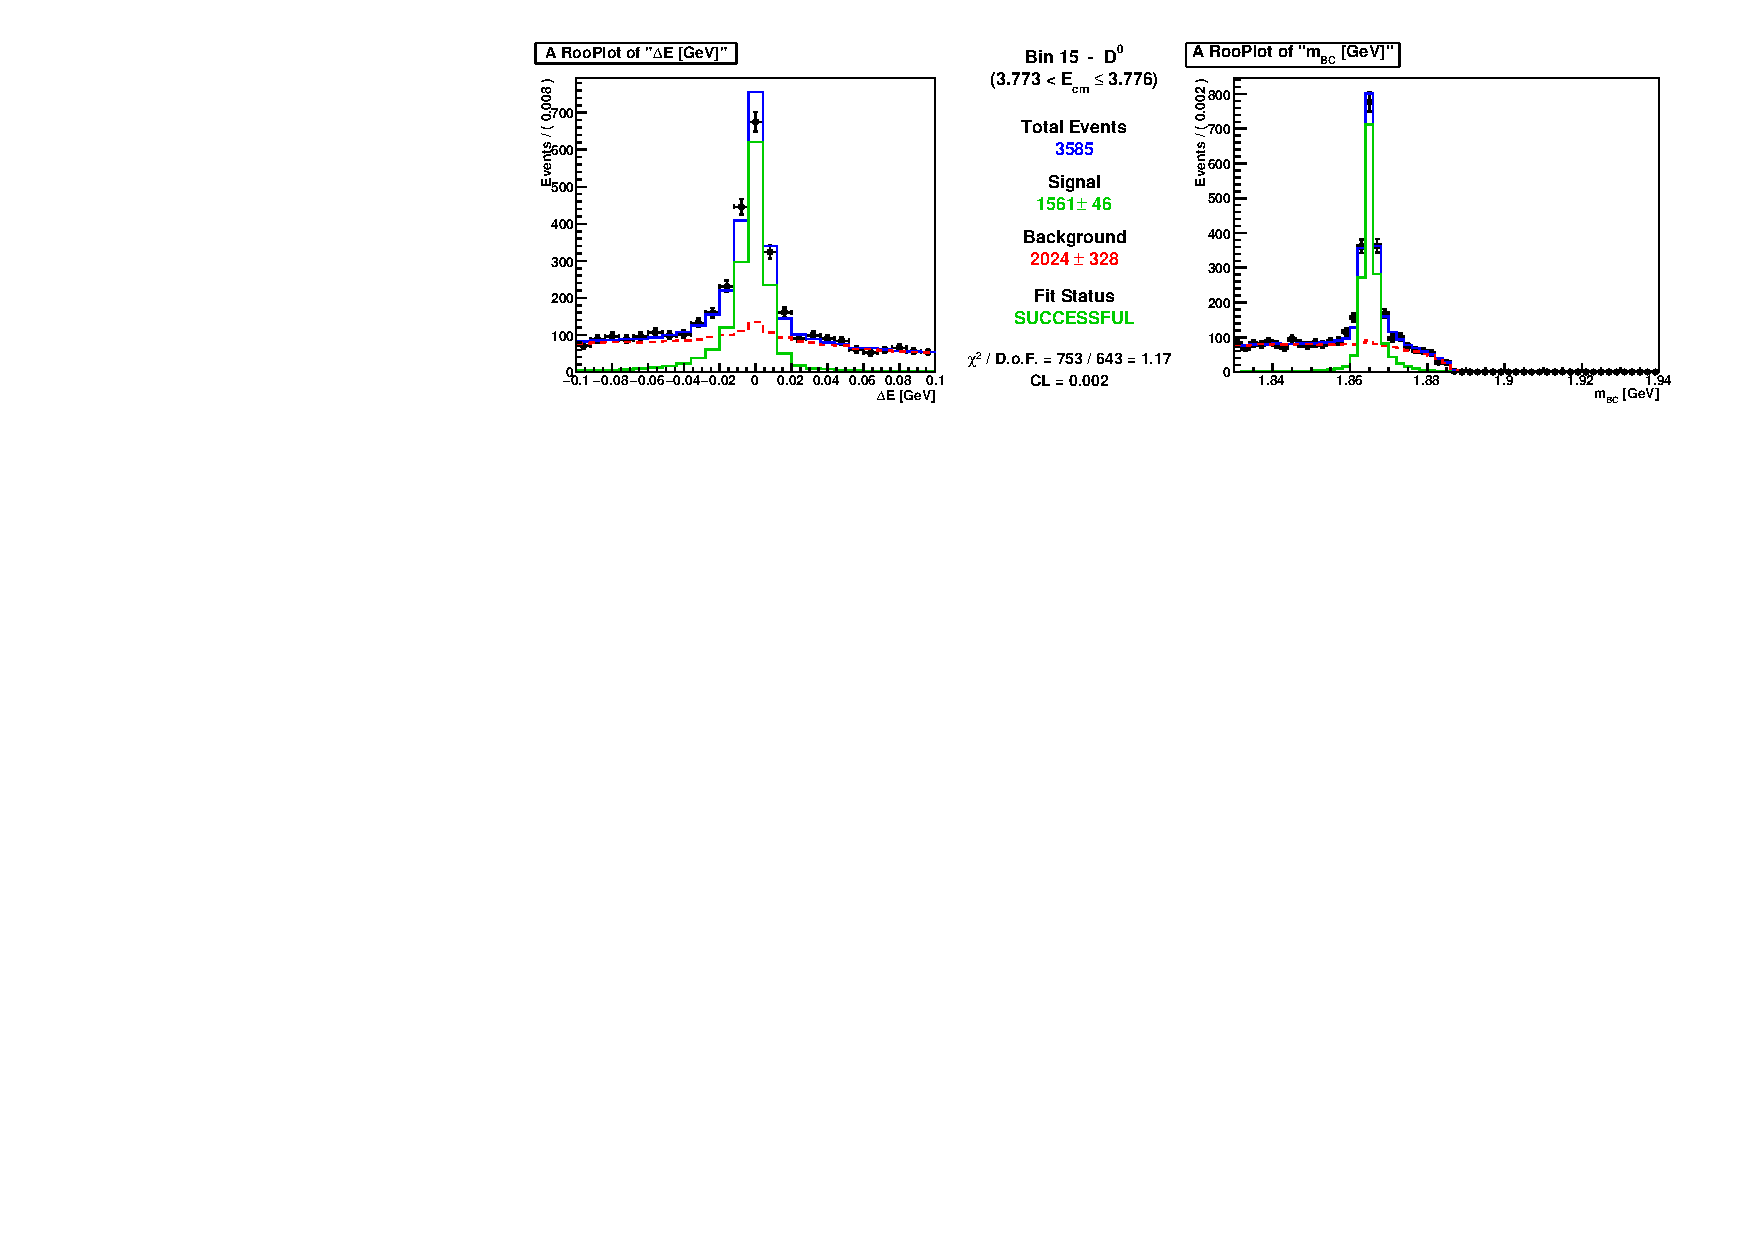
\includegraphics[scale=0.75]{figures/plots/fit_results/D0_bin_15.pdf}
\caption{An example 2D signal fit.}{The covers $\DO$ events in the region $\SI{3.773}{\GeV} < \Ecm \leq \SI{3.776}{\GeV}$.
The data points (black) are fitted by the total MC shape (blue), which is the sum of the signal (green) and background (red) components.}
\label{fig:example_fit}
\end{figure}


\section{Efficiency Correction}
\label{sec:efficiency}

In addition to the parameters gathered by \DTagAlg, truth information was taken from the generic $\DDbar$ samples in order to determine the mode-by-mode reconstruction efficiency.
To be deemed proper, a reconstruction must pass not only the standard $\Dtag$ cuts, but also match the generator information for the event.
This process removes peaking backgrounds from modes with similar constituents.
The total number of proper $\Dtag$ reconstructions is then divided by the number of $\D$ particles generated for each mode, and the mode-by-mode efficiencies are weighted by the PDG branching ratios \cite{ref:Olive:2014} to determine the overall efficiency ($\epsilon_{\D}$) for each of $\DO$ and $\Dp$:
\beq
\label{eq:DDbar_eff}
\epsilon_{D} = \sum_i \epsilon_i \, \mathcal{B}_i = \sum_i \left( \frac{ N_{i \text{ proper}} }{ N_{i \text{ generated}} } \right) \mathcal{B}_i.
\eeq
Each $\DO$ efficiency also includes the corresponding DCSD terms for its decay (See \Cref{sec:d_tagging}).

To determine the cross section at each point, this procedure was applied separately for each energy bin.
The total number of proper and generated particles for each energy bin are shown in \Cref{tab:DTag_eff_D0} for $\DO$ and \Cref{tab:DTag_eff_Dp_p1,tab:DTag_eff_Dp_p2} for $\Dp$.
The efficiencies for $\Dp$ and $\DO$ were also calculated across the total sample, and are shown for each mode in \Cref{tab:DTag_eff} and \Cref{fig:D_eff_by_mode}.
Each energy bin's total efficiency for both $\DO$ and $\Dp$ is shown in \Cref{tab:DTag_eff_E_bin}.

\begin{table}
\renewcommand\arraystretch{1.0}
\centering
\begin{tabular}{c|R{1.5cm}R{1.5cm}|R{1.5cm}R{1.5cm}|R{1.5cm}R{1.5cm}}
\hline
Bin & \multicolumn{2}{c|}{$\DOmodeA$} & \multicolumn{2}{c|}{$\DOmodeB$} & \multicolumn{2}{c}{$\DOmodeC$} \\
& $\Nprop$ & $\Ngen$ & $\Nprop$ & $\Ngen$ & $\Nprop$ & $\Ngen$ \\
\hline
 0 &   5519  &   7658  &  10757  &  27894  &   6927  &  16948  \\
 1 &  11203  &  15778  &  21753  &  56203  &  13704  &  33428  \\
 2 &   5470  &   7686  &  10761  &  27725  &   6929  &  16962  \\
 3 &  10987  &  15550  &  21357  &  55223  &  13639  &  33704  \\
 4 &  16311  &  23268  &  31913  &  83399  &  19997  &  50031  \\
 5 &  27586  &  38880  &  53505  & 138886  &  33927  &  83498  \\
 6 &  49416  &  69908  &  95785  & 250493  &  60813  & 150614  \\
 7 &  43530  &  62064  &  85248  & 222230  &  54013  & 134237  \\
 8 &  49056  &  70191  &  95402  & 250020  &  61035  & 150852  \\
 9 &  38764  &  54791  &  75237  & 194185  &  48307  & 116868  \\
10 &  55219  &  77765  & 107785  & 277958  &  69525  & 167368  \\
11 &  55412  &  78328  & 108229  & 278765  &  68944  & 167385  \\
12 &  38502  &  54639  &  75111  & 194082  &  48743  & 117181  \\
13 &  32802  &  46683  &  64440  & 166338  &  41593  & 100543  \\
14 &  21886  &  30983  &  43041  & 111230  &  27326  &  66506  \\
15 &  21849  &  31151  &  42979  & 110746  &  27406  &  66800  \\
16 &  16534  &  23429  &  31906  &  83165  &  20645  &  50035  \\
17 &  21963  &  31442  &  42724  & 110981  &  27807  &  67080  \\
18 &  27328  &  38791  &  53480  & 139055  &  34434  &  83489  \\
19 &  27019  &  38726  &  53396  & 139091  &  34605  &  83915  \\
20 &  38332  &  54586  &  75296  & 194835  &  47966  & 117143  \\
21 &  38032  &  54321  &  74841  & 195177  &  47764  & 117511  \\
22 &  43289  &  62110  &  84373  & 222186  &  53400  & 133871  \\
23 &  48974  &  70058  &  93686  & 249998  &  58965  & 150580  \\
24 &  32426  &  46536  &  62154  & 166927  &  38264  &  99797  \\
25 &  27022  &  38674  &  51590  & 138723  &  31748  &  83715  \\
26 &  16588  &  23491  &  30978  &  83656  &  19168  &  50246  \\
27 &  10832  &  15519  &  20060  &  55573  &  12281  &  33523  \\
28 &  10651  &  15284  &  20306  &  55439  &  12505  &  33815  \\
29 &  10980  &  15661  &  20233  &  55701  &  12405  &  33649  \\
30 &   5398  &   7822  &   9954  &  27637  &   6060  &  16711  \\
31 &   5425  &   7804  &  10010  &  27618  &   6156  &  16729  \\
32 &   5439  &   7830  &  10009  &  27799  &   5988  &  16695  \\
33 &  10659  &  15442  &  20070  &  55385  &  12282  &  33515  \\
34 &  10615  &  15443  &  19910  &  55573  &  12345  &  33592  \\
\hline
\end{tabular}
\caption{Number of proper and generated particles for $\DO$.}
{The mode-by-mode numbers of particles used in the efficiency calculations for $\DOmodeA, \DOmodeB,$ and $\DOmodeC$.}
\label{tab:DTag_eff_D0}
\end{table}


\begin{table}
\renewcommand\arraystretch{1.0}
\centering
\begin{tabular}{c|R{1.25cm}R{1.25cm}|R{1.25cm}R{1.25cm}|R{1.25cm}R{1.25cm}}
\hline
Bin & \multicolumn{2}{c|}{$\DpmodeA$} & \multicolumn{2}{c|}{$\DpmodeB$} & \multicolumn{2}{c}{$\DpmodeC$} \\
& $\Nprop$ & $\Ngen$ & $\Nprop$ & $\Ngen$ & $\Nprop$ & $\Ngen$ \\
\hline
 3 &  20022  &  37668  &   6600  &  24160  &   2272  &   5902  \\
 4 &  30234  &  56234  &  10010  &  36416  &   3431  &   8931  \\
 5 &  50966  &  93874  &  16855  &  60686  &   5750  &  14833  \\
 6 &  91414  & 169401  &  29807  & 109330  &  10199  &  26677  \\
 7 &  81267  & 150434  &  26528  &  96948  &   9060  &  23797  \\
 8 &  90448  & 168761  &  30206  & 109641  &  10233  &  26927  \\
 9 &  71896  & 131281  &  23901  &  85264  &   8167  &  20918  \\
10 & 103179  & 187949  &  34092  & 121352  &  11695  &  29969  \\
11 & 103605  & 188336  &  34331  & 122120  &  11672  &  29828  \\
12 &  72921  & 132064  &  23962  &  84947  &   8199  &  20937  \\
13 &  62056  & 112433  &  20547  &  72991  &   7021  &  17781  \\
14 &  41328  &  75280  &  13636  &  48338  &   4739  &  11979  \\
15 &  41441  &  75211  &  13640  &  48504  &   4613  &  11861  \\
16 &  31212  &  56487  &  10309  &  36655  &   3513  &   8982  \\
17 &  41621  &  75045  &  13881  &  49145  &   4680  &  12048  \\
18 &  51909  &  94077  &  16905  &  60819  &   5769  &  14879  \\
19 &  52042  &  94156  &  17035  &  60618  &   5885  &  14977  \\
20 &  72086  & 131300  &  23647  &  84907  &   8286  &  21035  \\
21 &  72509  & 131694  &  23555  &  84570  &   8029  &  20806  \\
22 &  82597  & 150805  &  26792  &  96787  &   9334  &  23503  \\
23 &  92228  & 169069  &  29808  & 109702  &  10559  &  26985  \\
24 &  61616  & 113123  &  19611  &  73321  &   6985  &  18018  \\
25 &  50613  &  93767  &  16383  &  60811  &   5712  &  14759  \\
26 &  30736  &  56653  &   9583  &  36280  &   3614  &   9245  \\
27 &  20427  &  37582  &   6456  &  24186  &   2250  &   5811  \\
28 &  20295  &  37687  &   6536  &  24289  &   2214  &   5811  \\
29 &  20393  &  37337  &   6489  &  24201  &   2466  &   6167  \\
30 &  10309  &  18737  &   3128  &  12099  &   1159  &   3003  \\
31 &  10345  &  18895  &   3216  &  12023  &   1120  &   2946  \\
32 &  10142  &  18893  &   3213  &  12066  &   1168  &   3020  \\
33 &  20265  &  37114  &   6374  &  24194  &   2330  &   5967  \\
34 &  20311  &  37337  &   6362  &  24378  &   2326  &   6057  \\
\hline
\end{tabular}
\caption{Number of proper and generated particles for $\Dp$ (part 1).}
{The mode-by-mode numbers of particles used in the efficiency calculations for $\DpmodeA, \DpmodeB,$ and $\DpmodeC$.}
\label{tab:DTag_eff_Dp_p1}
\end{table}


\begin{table}
\renewcommand\arraystretch{1.0}
\centering
\begin{tabular}{c|R{1.25cm}R{1.25cm}|R{1.25cm}R{1.25cm}|R{1.25cm}R{1.25cm}}
\hline
Bin & \multicolumn{2}{c|}{$\DpmodeD$} & \multicolumn{2}{c|}{$\DpmodeE$} & \multicolumn{2}{c}{$\DpmodeF$} \\
& $\Nprop$ & $\Ngen$ & $\Nprop$ & $\Ngen$ & $\Nprop$ & $\Ngen$ \\
\hline
 3 &   5578  &  27502  &   3414  &  14899  &   1698  &   3980  \\
 4 &   8468  &  41353  &   4999  &  22340  &   2485  &   5867  \\
 5 &  14556  &  69102  &   8309  &  37104  &   4344  &   9959  \\
 6 &  25432  & 124123  &  14807  &  66943  &   7430  &  17744  \\
 7 &  22850  & 110296  &  13319  &  60059  &   6723  &  15843  \\
 8 &  25820  & 124151  &  15057  &  66954  &   7478  &  17655  \\
 9 &  20373  &  96362  &  11898  &  52068  &   6093  &  13955  \\
10 &  29030  & 138372  &  17076  &  74519  &   8425  &  19594  \\
11 &  29195  & 137508  &  17221  &  74539  &   8534  &  19799  \\
12 &  20216  &  96603  &  12006  &  52123  &   5985  &  13833  \\
13 &  17507  &  82589  &  10228  &  44534  &   5111  &  11746  \\
14 &  11705  &  54998  &   6839  &  29643  &   3429  &   7891  \\
15 &  11602  &  55245  &   6810  &  29770  &   3461  &   7989  \\
16 &   8763  &  41572  &   4963  &  22250  &   2564  &   5876  \\
17 &  11651  &  55576  &   6953  &  29754  &   3341  &   7827  \\
18 &  14509  &  68677  &   8617  &  37138  &   4235  &   9867  \\
19 &  14565  &  68864  &   8466  &  36828  &   4361  &   9826  \\
20 &  20572  &  97073  &  12192  &  52476  &   6187  &  13850  \\
21 &  20411  &  96827  &  11748  &  52152  &   5898  &  13671  \\
22 &  23090  & 109958  &  13325  &  59244  &   6906  &  15913  \\
23 &  25746  & 124249  &  14667  &  66799  &   7601  &  17652  \\
24 &  17179  &  82921  &   9571  &  44714  &   4994  &  11729  \\
25 &  14120  &  69390  &   7922  &  37132  &   4165  &   9905  \\
26 &   8380  &  41424  &   4794  &  22343  &   2562  &   5908  \\
27 &   5593  &  27680  &   3072  &  14738  &   1694  &   3935  \\
28 &   5627  &  27587  &   3151  &  14791  &   1657  &   3859  \\
29 &   5677  &  27727  &   3118  &  14862  &   1700  &   3924  \\
30 &   2863  &  13875  &   1604  &   7514  &    849  &   2003  \\
31 &   2733  &  13650  &   1554  &   7495  &    828  &   1971  \\
32 &   2808  &  13903  &   1491  &   7273  &    876  &   2005  \\
33 &   5572  &  27708  &   3168  &  14898  &   1659  &   3890  \\
34 &   5627  &  27755  &   3095  &  14821  &   1692  &   3962  \\
\hline
\end{tabular}
\caption{Number of proper and generated particles for $\Dp$ (part 2).}
{The mode-by-mode numbers of particles used in the efficiency calculations for $\DpmodeD, \DpmodeE,$ and $\DpmodeF$.}
\label{tab:DTag_eff_Dp_p2}
\end{table}


\begin{table}[h]
\centering
\begin{tabular}{l c c}
\hline
Decay Mode ($i$) & PDG $\mathcal{B}_i$ [\%] & MC Efficiency $\epsilon_i$ \\
\hline
$\DOmodeA$ & \pp 3.89 $\pm$ 0.05 & 0.70226(74) \\ 
$\DOmodeB$ &    13.93 $\pm$ 0.50 & 0.38190(29) \\ 
$\DOmodeC$ & \pp 8.11 $\pm$ 0.20 & 0.40277(38) \\ 
\hline
\multicolumn{3}{c}{$\epsilon_{\DO}$ = (11.320 $\pm$ 0.213)\%} \\
\hline
$\DpmodeA$ & \pp 9.13 $\pm$ 0.19 & 0.54699(42)\pp \\
$\DpmodeB$ & \pp 5.99 $\pm$ 0.18 & 0.27570(38)\pp \\
$\DpmodeC$ & \pp 1.47 $\pm$ 0.07 & 0.38972(89)\pp \\
$\DpmodeD$ & \pp 6.99 $\pm$ 0.27 & 0.20864(31)\pp \\
$\DpmodeE$ & \pp 3.12 $\pm$ 0.11 & 0.22540(43)\pp \\
$\DpmodeF$ & \pp 0.95 $\pm$ 0.03 & 0.43199(116)   \\
\hline
\multicolumn{3}{c}{$\epsilon_{\Dp}$ = (9.792 $\pm$ 0.134)\%} \\[1pt]
\hline
\end{tabular}
\caption{Mode-by-mode reconstruction efficiencies for $\DO$ and $\Dp$.}
{The values shown are over the entire data sample, while calculations for the cross sections use the values of each energy point individually.}
\label{tab:DTag_eff}
\end{table}


\begin{figure}[h]
\centering
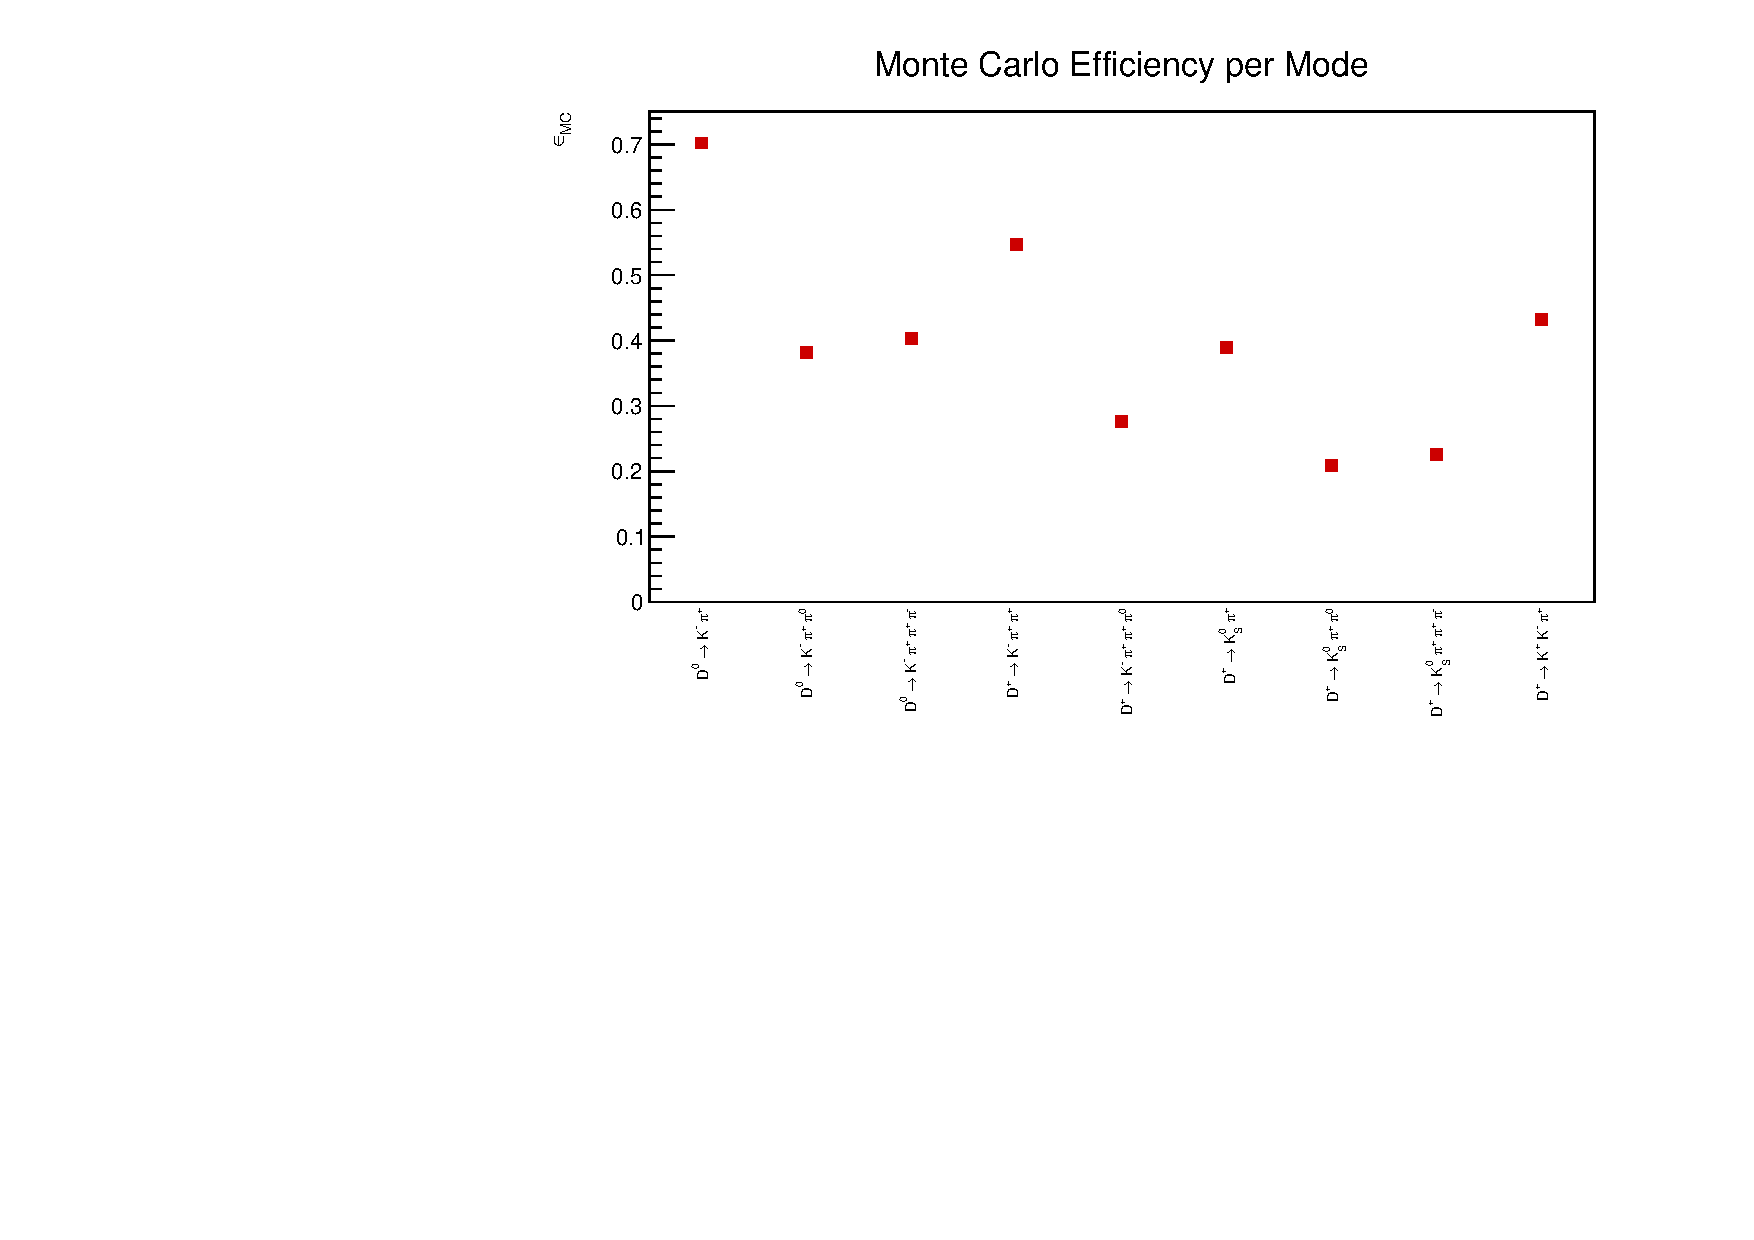
\includegraphics[scale=0.8]{figures/plots/D_eff_by_mode.pdf}
\caption{Mode-by-mode MC efficiencies for $\DO$ and $\Dp$.}
{The error bars are negligible on the scale shown.}
\label{fig:D_eff_by_mode}
\end{figure}


\begin{table}
\centering
\renewcommand\arraystretch{1.0}
\begin{tabular}{c C{3cm} C{3cm}}
\hline
$E_{\text{bin}}$ & $\epsilon_{\DO}$ & $\epsilon_{\Dp}$ \\
\hline
 0 & 0.1149 $\pm$ 0.0023 & -                   \\ 
 1 & 0.1148 $\pm$ 0.0022 & -                   \\ 
 2 & 0.1149 $\pm$ 0.0023 & -                   \\ 
 3 & 0.1142 $\pm$ 0.0022 & 0.0959 $\pm$ 0.0014 \\ 
 4 & 0.1130 $\pm$ 0.0022 & 0.0965 $\pm$ 0.0014 \\ 
 5 & 0.1142 $\pm$ 0.0022 & 0.0978 $\pm$ 0.0014 \\ 
 6 & 0.1135 $\pm$ 0.0021 & 0.0964 $\pm$ 0.0013 \\ 
 7 & 0.1134 $\pm$ 0.0021 & 0.0968 $\pm$ 0.0013 \\ 
 8 & 0.1132 $\pm$ 0.0021 & 0.0966 $\pm$ 0.0013 \\ 
 9 & 0.1150 $\pm$ 0.0022 & 0.0986 $\pm$ 0.0014 \\ 
10 & 0.1153 $\pm$ 0.0022 & 0.0986 $\pm$ 0.0014 \\ 
11 & 0.1150 $\pm$ 0.0022 & 0.0990 $\pm$ 0.0014 \\ 
12 & 0.1151 $\pm$ 0.0022 & 0.0990 $\pm$ 0.0014 \\ 
13 & 0.1149 $\pm$ 0.0022 & 0.0992 $\pm$ 0.0014 \\ 
14 & 0.1147 $\pm$ 0.0022 & 0.0991 $\pm$ 0.0014 \\ 
15 & 0.1146 $\pm$ 0.0022 & 0.0988 $\pm$ 0.0014 \\ 
16 & 0.1144 $\pm$ 0.0022 & 0.0989 $\pm$ 0.0014 \\ 
17 & 0.1144 $\pm$ 0.0022 & 0.0993 $\pm$ 0.0014 \\
18 & 0.1144 $\pm$ 0.0022 & 0.0988 $\pm$ 0.0014 \\
19 & 0.1141 $\pm$ 0.0022 & 0.0993 $\pm$ 0.0014 \\
20 & 0.1144 $\pm$ 0.0022 & 0.0989 $\pm$ 0.0014 \\
21 & 0.1136 $\pm$ 0.0022 & 0.0985 $\pm$ 0.0014 \\
22 & 0.1124 $\pm$ 0.0021 & 0.0983 $\pm$ 0.0014 \\
23 & 0.1112 $\pm$ 0.0021 & 0.0973 $\pm$ 0.0014 \\
24 & 0.1101 $\pm$ 0.0021 & 0.0967 $\pm$ 0.0014 \\
25 & 0.1098 $\pm$ 0.0021 & 0.0960 $\pm$ 0.0014 \\
26 & 0.1100 $\pm$ 0.0021 & 0.0961 $\pm$ 0.0014 \\
27 & 0.1072 $\pm$ 0.0021 & 0.0960 $\pm$ 0.0014 \\
28 & 0.1081 $\pm$ 0.0021 & 0.0959 $\pm$ 0.0014 \\
29 & 0.1078 $\pm$ 0.0021 & 0.0968 $\pm$ 0.0014 \\
30 & 0.1064 $\pm$ 0.0021 & 0.0965 $\pm$ 0.0015 \\
31 & 0.1074 $\pm$ 0.0021 & 0.0961 $\pm$ 0.0015 \\
32 & 0.1063 $\pm$ 0.0021 & 0.0953 $\pm$ 0.0015 \\
33 & 0.1071 $\pm$ 0.0021 & 0.0961 $\pm$ 0.0014 \\
34 & 0.1065 $\pm$ 0.0021 & 0.0957 $\pm$ 0.0014 \\
\hline
\end{tabular}
\caption{The overall reconstruction efficiency of $\DO$ and $\Dp$ for each energy bin.}
{These values are used to calculate the corresponding cross sections at each energy point.  The listed errors are statistical only.}
\label{tab:DTag_eff_E_bin}
\end{table}


\subsection{$\sCP$ Violation Correction}
\label{ssec:cp_correction}

Due to $\sCP$ violation in the $\DO \aDO$ system, each of the neutral decay modes must be corrected to account for quantum correlations.
This is done by applying scaling factors to the efficiency for each of the three modes used in reconstruction.
The corrections are parameterized for each mode ($m$) by the following form \cite{ref:Asner:2008}:
\beq
\label{eq:qc}
\alpha_{\DO \rightarrow m} = 1 + r_m^2 + 2 \times y \times r_m \times R_m \times \cos(\delta_m).
\eeq
Here, $r_m$ and $\delta_m$ represent the relative magnitudes and phases between the Cabbibo-favored and doubly-Cabbibo-suppressed modes, respectively, while the factor of $R_m$ represents a coherence factor characterizing the variation of $\delta_m$ over phase space.
Note, there is no such variation for a two-body decay (like $\DOmodeA$), so $R_{\DOmodeA} = 1$.
The value of $y$ represents the difference in total width components of the $\DO \aDO$ system, $y = (\Gamma_2 - \Gamma_1) / (\Gamma_2 + \Gamma_1)$, where 1 and 2 represent the $\sCP$-odd and $\sCP$-even states, respectively.

The mode-dependent values for these factors are listed in \Cref{tab:qc_factors}.
These are taken from the $CPV$-allowed values in \cite{ref:HFAG:2015} for $\DOmodeA$, and from \cite{ref:Evans:2016} for $\DOmodeB$ and $\DOmodeC$.
The value of $y = 0.0066^{+0.0007}_{-0.0010}$ is also from \cite{ref:HFAG:2015}, and is the same for all modes.
After applying each of the mode-dependent corrections, the efficiency for the full sample changes from $\epsilon_{\DO} = (11.320 \pm 0.213)\%$ to $\epsilon_{\DO} = (11.352 \pm 0.213)\%$, and similarly for the efficiencies of each $\Ecm$ bin.

\begin{table}[h]
\renewcommand\arraystretch{1.0}
\begin{tabular}{l|r@{$\;\pm\;$}l r@{~}l r@{~}l|r@{~}l}
\hline 
\multicolumn{1}{c|}{Mode}  & \multicolumn{2}{c}{$r_m$} & \multicolumn{2}{c}{$R_m$} & \multicolumn{2}{c|}{$\delta_m$ [\si{^\circ}]} & \multicolumn{2}{c}{$\alpha_m$} \\
\hline
$\DOmodeA$ & 0.0591 & 0.0063 & \multicolumn{2}{c}{1}         &  11.8 & $^{+\;\pp 9.5}_{-\;14.7}$ & 1.00426 & $ \pm\; 0.00083$             \\
$\DOmodeB$ & 0.0447 & 0.0012 & 0.81 & $\pm\; 0.06$           &  18   & $^{+\;   14  }_{-\;15  }$ & 1.00248 & $ \pm\; 0.00014$             \\
$\DOmodeC$ & 0.0549 & 0.0006 & 0.43 & $^{+\;0.17}_{-\;0.13}$ & -52   & $^{+\;   28  }_{-\;17  }$ & 1.00270 & $^{+\;0.00014}_{-\;0.00012}$ \\
\hline 
\end{tabular}
\caption{The quantum correlated factors for the $\DO$ modes.}
\label{tab:qc_factors}
\end{table}


\section{Fitting Procedure}
\label{sec:fitting}

After applying the correction in \Cref{ssec:cp_correction}, the efficiency values (\Cref{tab:DTag_eff_E_bin}) were combined with the luminosity (\Cref{tab:luminosity}) and the signal values from each 2D fit (\Cref{tab:xsec_rc_data}) to determine the cross section at each energy point.  Since each $\psipp$ produces a $\DDbar$ pair, a factor of 2 is included to avoid double counting:
\beq
\label{eq:xsec_rc_data}
\sigma_{\DDbar}^{RC}(E_i) = \frac{ N_D(E_i) }{ 2 \, \epsilon_D(E_i) \, \mathcal{L}(E_i) }.
\eeq
The resulting cross section values for $\DO$ and $\Dp$ are also listed in \Cref{tab:xsec_rc_data}, and shown in \Cref{fig:xsec_rc_data}.


\begin{table}%[h]
\centering
\begin{tabular}{c r@{$\;\pm\;$}l r@{$\;\pm\;$}l r@{$\;\pm\;$}l r@{$\;\pm\;$}l}
\hline
$E_{\text{mid}}$ & \multicolumn{2}{c}{$N_{\DO \aDO}$} & \multicolumn{2}{c}{$\sigma^{RC}_{\DO \aDO}$ [\si{\nb}]} & \multicolumn{2}{c}{$N_{\Dp \Dm}$}  & \multicolumn{2}{c}{$\sigma^{RC}_{\Dp \Dm}$ [\si{\nb}]} \\
\hline
3.7355 &   12 &  5 & 0.155 & 0.065 & \multicolumn{2}{c}{-} & \multicolumn{2}{c}{-} \\ 
3.7364 &   24 &  7 & 0.212 & 0.066 & \multicolumn{2}{c}{-} & \multicolumn{2}{c}{-} \\ 
3.7377 &   15 &  5 & 0.204 & 0.069 & \multicolumn{2}{c}{-} & \multicolumn{2}{c}{-} \\ 
3.7447 &  166 & 15 & 0.761 & 0.072 &   27 &  6 & 0.147 & 0.038 \\ 
3.7464 &  266 & 20 & 0.823 & 0.064 &   98 & 12 & 0.361 & 0.046 \\  
3.7485 &  508 & 27 & 0.970 & 0.056 &  199 & 17 & 0.446 & 0.040 \\ 
3.7503 &  825 & 34 & 1.210 & 0.055 &  321 & 22 & 0.555 & 0.039 \\ 
3.7525 & 1012 & 38 & 1.334 & 0.057 &  479 & 27 & 0.743 & 0.043 \\ 
3.7541 & 1143 & 41 & 1.462 & 0.059 &  510 & 28 & 0.767 & 0.044 \\ 
3.7556 & 1454 & 45 & 1.622 & 0.059 &  680 & 32 & 0.887 & 0.044 \\ 
3.7586 & 1993 & 53 & 1.940 & 0.064 & 1036 & 39 & 1.177 & 0.048 \\ 
3.7616 & 2388 & 58 & 2.303 & 0.071 & 1323 & 44 & 1.493 & 0.054 \\ 
3.7646 & 2016 & 53 & 2.662 & 0.086 & 1224 & 42 & 1.884 & 0.070 \\ 
3.7675 & 1719 & 48 & 3.051 & 0.104 & 1050 & 38 & 2.174 & 0.086 \\ 
3.7705 & 1578 & 46 & 3.391 & 0.119 & 1044 & 38 & 2.610 & 0.103 \\ 
3.7735 & 1561 & 46 & 3.708 & 0.131 & 1116 & 39 & 3.086 & 0.118 \\ 
3.7765 & 1543 & 45 & 3.673 & 0.130 & 1108 & 39 & 3.058 & 0.118 \\ 
3.7795 & 1522 & 46 & 3.372 & 0.121 & 1001 & 38 & 2.579 & 0.105 \\
3.7826 & 1398 & 44 & 2.826 & 0.106 &  957 & 38 & 2.248 & 0.095 \\
3.7855 & 1140 & 41 & 1.948 & 0.080 &  806 & 36 & 1.589 & 0.075 \\
3.7885 &  848 & 38 & 1.310 & 0.064 &  645 & 34 & 1.147 & 0.064 \\
3.7925 &  725 & 37 & 0.903 & 0.050 &  480 & 30 & 0.688 & 0.045 \\
3.7964 &  514 & 35 & 0.561 & 0.040 &  321 & 31 & 0.403 & 0.040 \\
3.8005 &  354 & 31 & 0.404 & 0.037 &  182 & 28 & 0.238 & 0.037 \\
3.8036 &  194 & 23 & 0.324 & 0.039 &  117 & 22 & 0.223 & 0.043 \\
3.8065 &  125 & 19 & 0.323 & 0.050 &   95 & 16 & 0.280 & 0.050 \\
3.8095 &   57 & 13 & 0.206 & 0.048 &   33 & 13 & 0.138 & 0.055 \\
3.8124 &   11 &  9 & 0.056 & 0.050 &   29 & 11 & 0.168 & 0.065 \\
3.8157 &    6 &  7 & 0.046 & 0.050 &    8 &  8 & 0.067 & 0.062 \\
3.8237 &   11 &  7 & 0.128 & 0.081 &   15 &  8 & 0.196 & 0.108 \\
3.8315 &    7 &  5 & 0.118 & 0.086 &    2 &  6 & 0.039 & 0.114 \\
3.8397 &   15 &  6 & 0.254 & 0.108 &   12 &  6 & 0.239 & 0.119 \\
3.8475 &   14 &  6 & 0.250 & 0.109 &    9 &  6 & 0.172 & 0.121 \\
3.8556 &   26 &  8 & 0.377 & 0.117 &   16 &  6 & 0.269 & 0.108 \\
3.8636 &   15 &  6 & 0.236 & 0.099 &    7 &  5 & 0.138 & 0.095 \\
\hline
\end{tabular} 
\caption{The $\DDbar$ cross section at each $\Ecm$ point.}
{The number of data events observed in each $\Ecm$ bin are also shown.
The uncertainties on the cross sections are statistical only and come from the signal fitting ($N_D$), PDG values (\Cref{tab:DTag_eff}), and MC reconstruction efficiency (\Cref{tab:DTag_eff_E_bin}).
The values for $N_{\DO \aDO}$ and $N_{\Dp \Dm}$ are taken from the signal fits shown in \Cref{app:D0_signal_fits,app:Dp_signal_fits}.}
\label{tab:xsec_rc_data}
\end{table}


\begin{figure}[h]
\centering
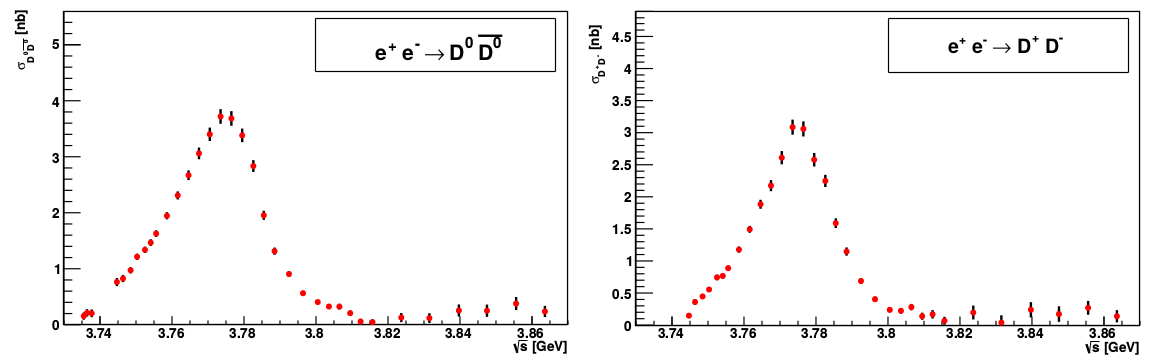
\includegraphics[scale=0.35]{figures/plots/xsec_data.png}
\caption{The measured $\ee \rightarrow \DDbar$ cross sections.}
{The $\DO \aDO$ cross section is shown on the left and $\Dp \Dm$ is shown on the right. }
\label{fig:xsec_rc_data}
\end{figure}


Using the measured $\DDbar$ cross sections, we fit to \Cref{eq:xsec_rc_simp} using each of the form factor choices described in \Cref{sec:form_factors}.
In each case, there are four common fit parameters: $\Mpsipp$, $\Gpsipp$, $\Geepsipp$, and $\Ppsipp$.
These represent the mass, total width, electron partial width, and relative phase to the non-resonant contribution for the $\psipp$, respectively.
This notation for the total width corresponds to $\Gamma(M)$ in \Cref{sec:xsec_derivation}.
Two additional fitting parameters are dependent on which form factor is being used: $F_{NR}$ and $a_{NR}$ for the exponential, or $\Gpsip$ and $F_0$ for the VDM.
For the former, these represent the amplitude and exponent normalization for the non-resonant contribution.
In the latter case, these represent the modified total width for the $\psip$ above resonance (see \Cref{sec:form_factors}) and the constant contribution of resonances above the $\psipp$.
The fitting is done simultaneously for $\DO$ and $\Dp$ with identical parameters using TMinuit with a $\chi^2$ minimization.
The value minimized is the sum of the $\chi^2$ values from each of the $\DO$ and $\Dp$ cross section functions.  
Results for the Exponential and VDM choices are shown in \Cref{fig:exp_results,fig:vdm_results}, respectively.


\begin{figure}[H]
\centering
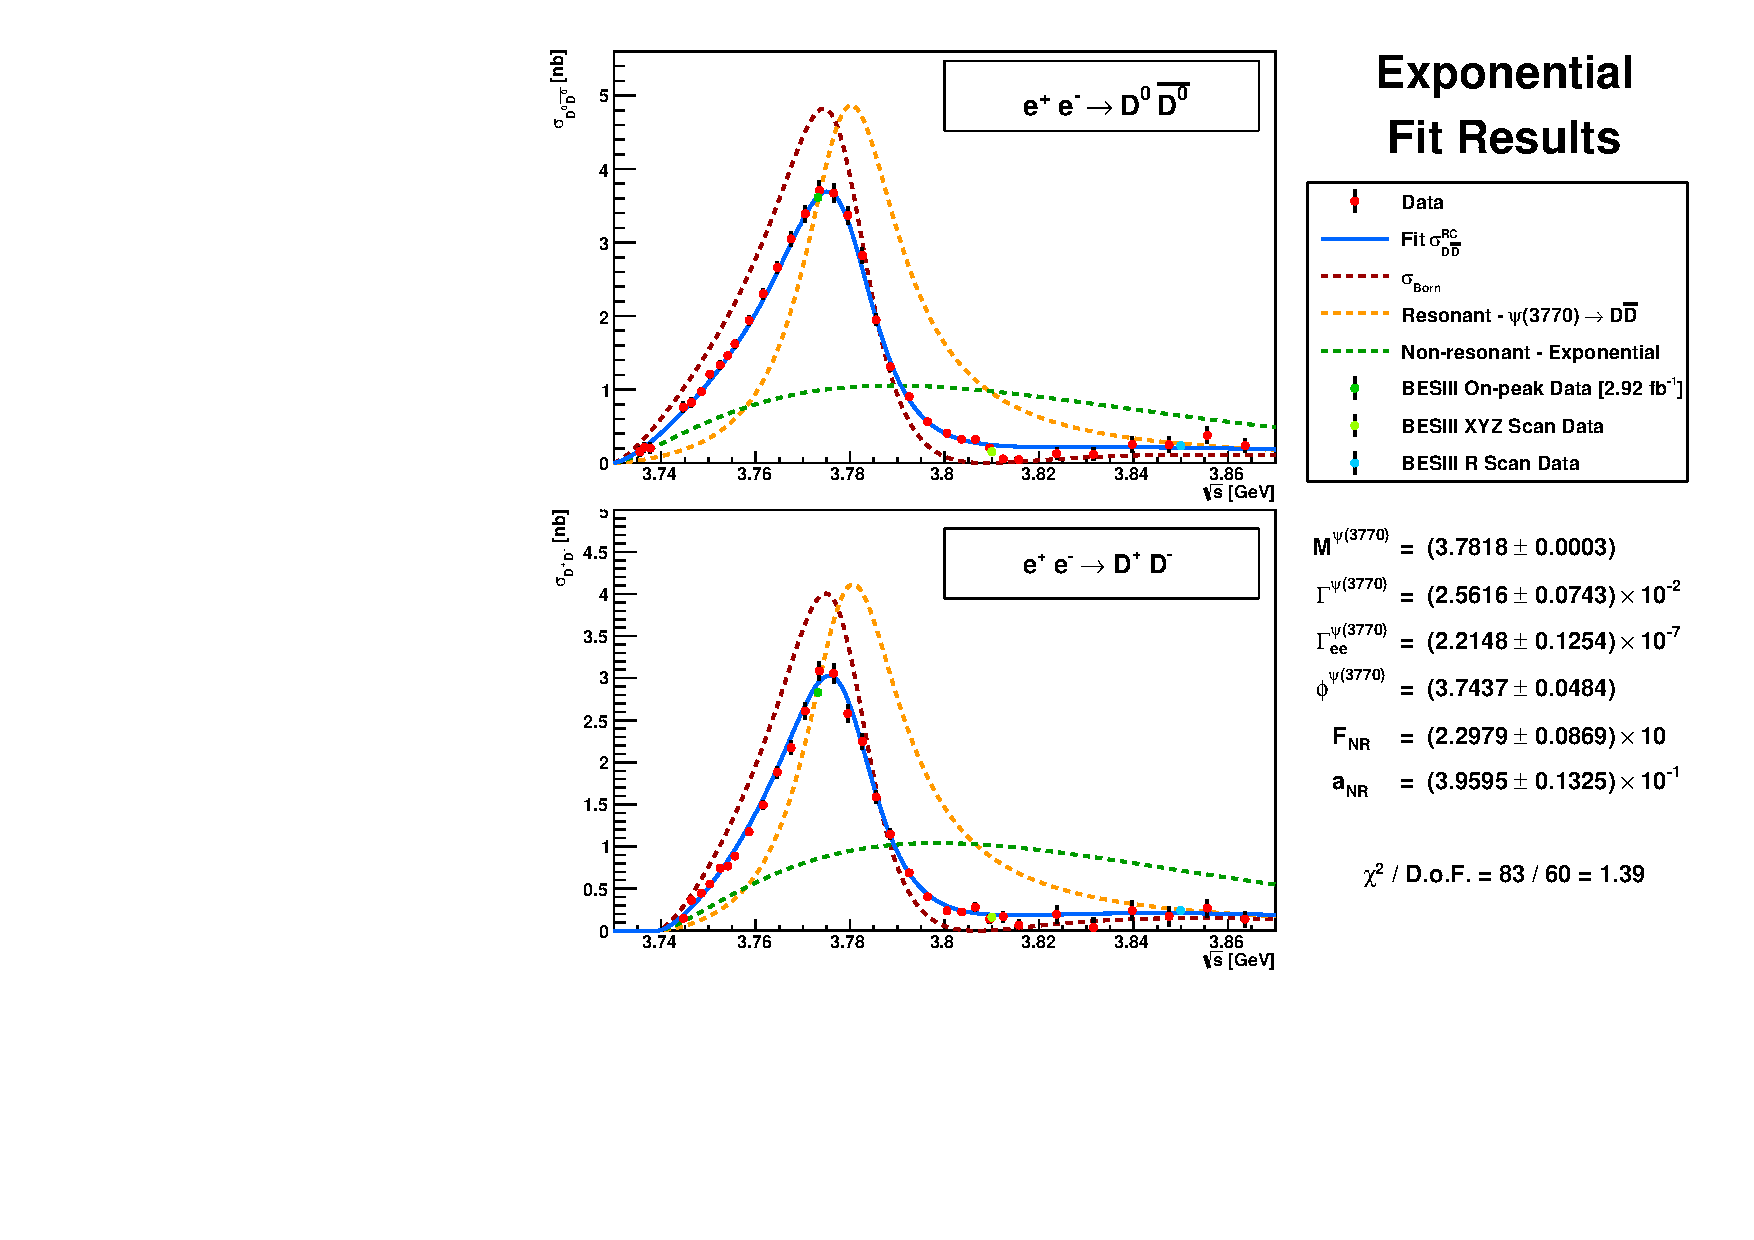
\includegraphics[scale=0.75]{figures/plots/lineshape_exp.pdf}
\caption{The Exponential Model fit results.}
{The results for $\DO$ are shown on the top and the results for $\Dp$ are shown on the bottom. The fit shape (blue) is calculated from \Cref{eq:xsec_rc} using the non-resonant component from \Cref{eq:exp_model}.}
\label{fig:exp_results}
\end{figure}

\begin{figure}%[h]
\centering
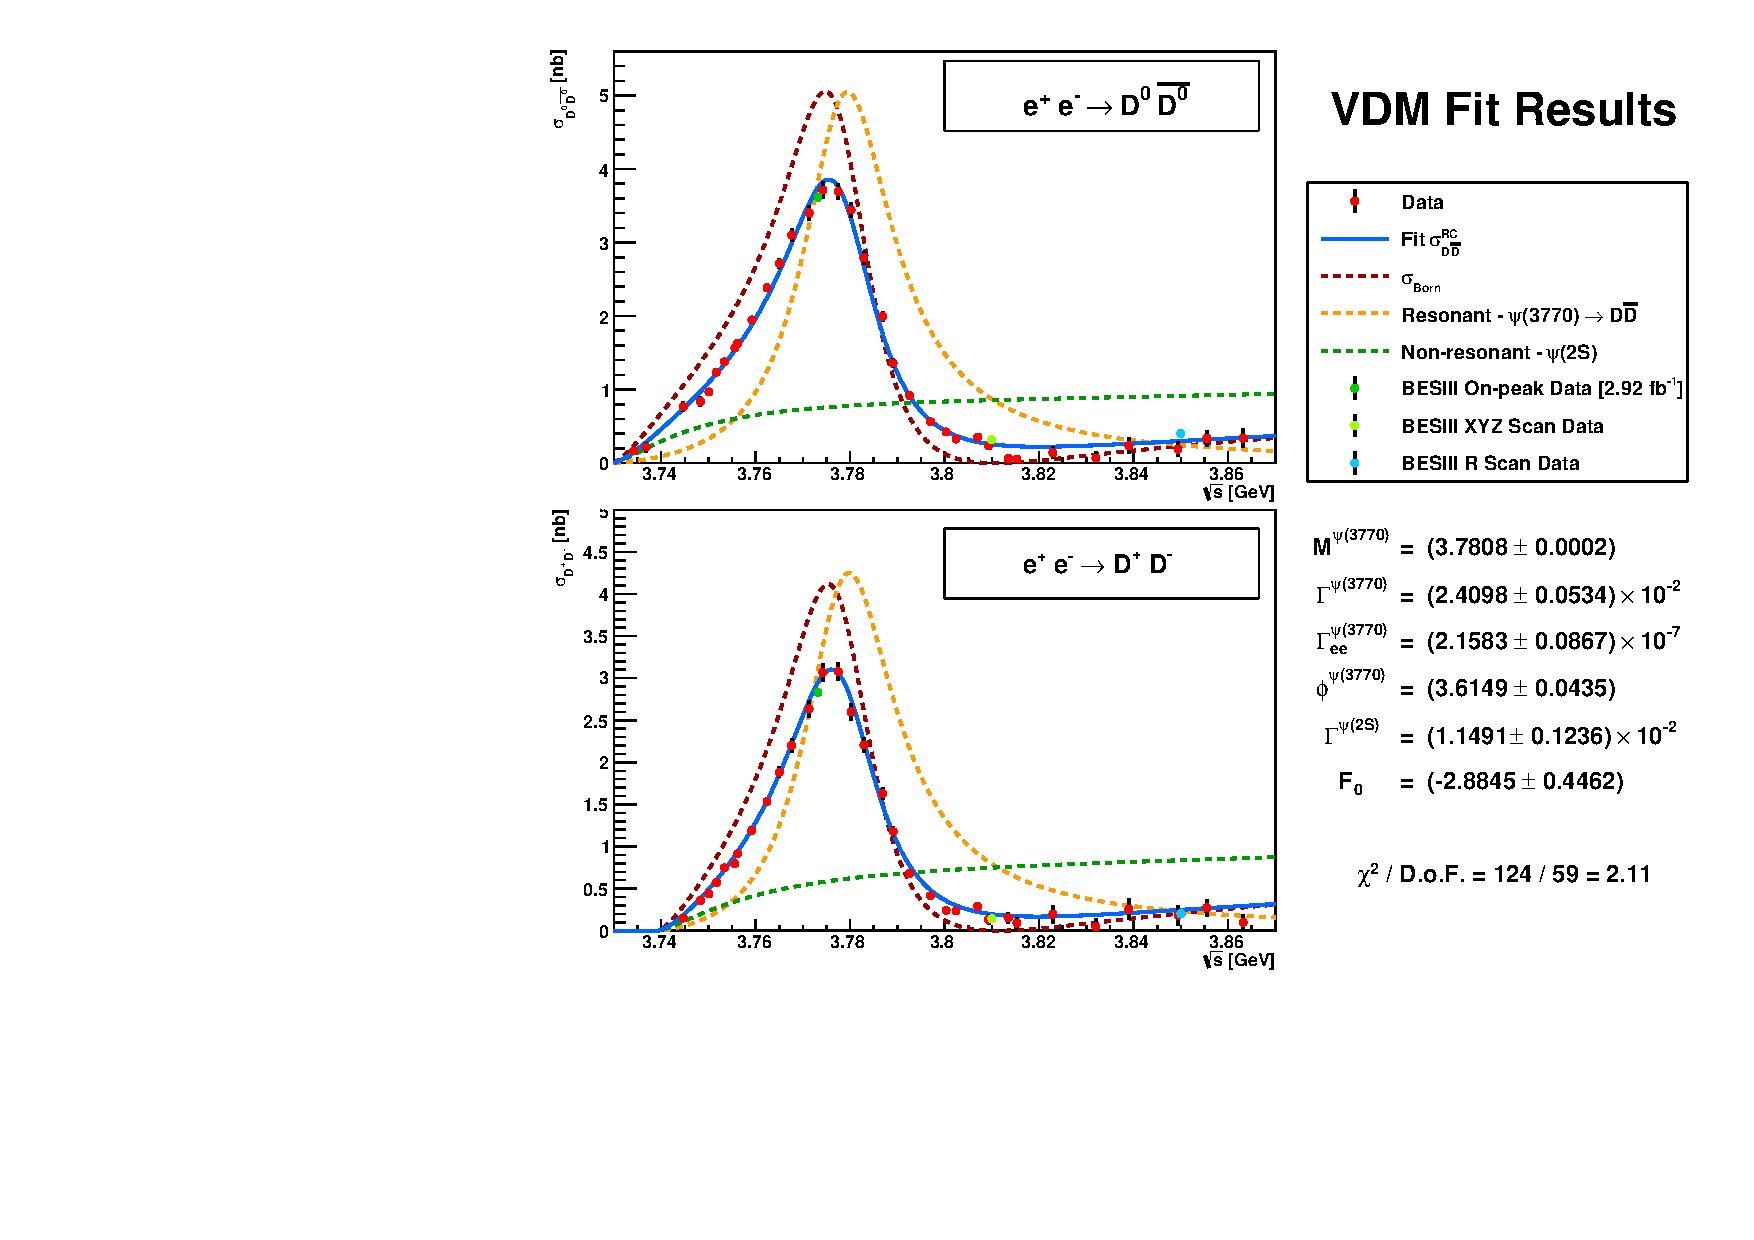
\includegraphics[scale=0.75]{figures/plots/lineshape_vdm.pdf}
\caption{The Vector Dominance Model fit results.}
{The results for $\DO$ are shown on the top and the results for $\Dp$ are shown on the bottom. The fit shape (blue) is calculated from \Cref{eq:xsec_rc} using the non-resonant component from \Cref{eq:vdm_model}.}
\label{fig:vdm_results}
\end{figure}


\subsection{Coulomb Correction}
\label{ssec:coulomb}

In the development of this analysis, it was discovered that the theoretical formulation in \Cref{sec:xsec_derivation} did not lead to a successful fit of the $\DDbar$ cross sections, shown in \Cref{fig:vdm_Coulomb}.
Namely, including the Coulomb effect pulls the $\DO \aDO$ and $\Dp \Dm$ cross sections in opposite directions.
We found the best fits were achieved by altering \Cref{eq:z_Dp} to set the Coulomb factor to 1.
While this disagrees with conventional theoretical wisdom, it is consistent with studies of $\Upsilon(4S) \rightarrow B\overline{B}$ where applying a Coulomb correction for the charged final state also leads to inconsistency with data.

\begin{figure}%[h]
\centering
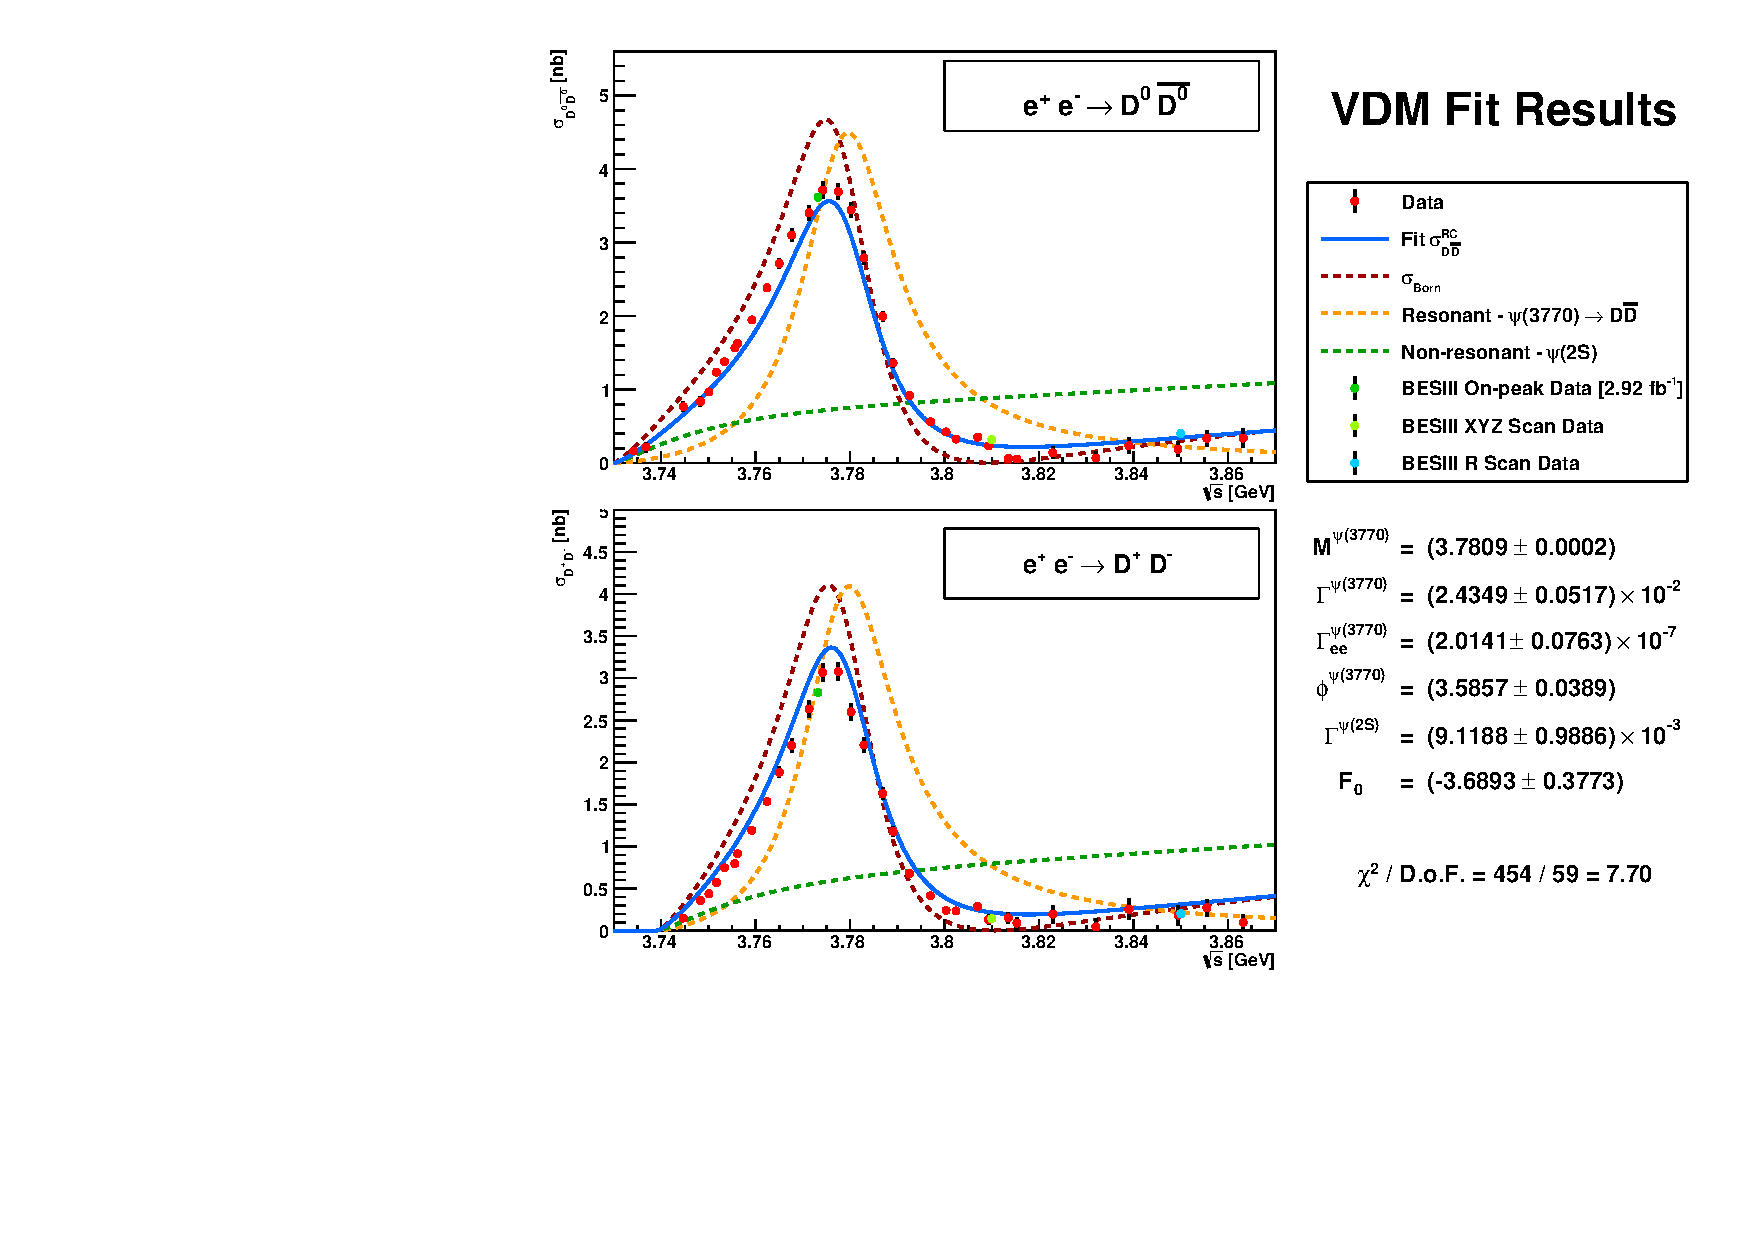
\includegraphics[scale=0.75]{figures/plots/lineshape_vdm_Coulomb.pdf}
\caption{The Vector Dominance Model fit results with Coulomb interactions.}
{The results for $\DO$ are shown on the top and the results for $\Dp$ are shown on the bottom.  Including this factor provides notably worse results than when excluding it (see \Cref{fig:vdm_results}).}
\label{fig:vdm_Coulomb}
\end{figure}

This is most clearly seen in the ratio of $\Dp \Dm$ and $\DO \aDO$ cross sections, shown in \Cref{fig:Coulomb_ratio}, where the `No Coulomb' method sets $\zDD$ in \Cref{eq:xsec_rc_simp,eq:Gamma} to unity, the `Partial Coulomb' sets this factor to unity only for \Cref{eq:xsec_rc_simp}, and the `Full Coulomb' is the default assumption.
Agreement of the measured cross section ratio with the `No Coulomb' calculation is substantially better.
This is also true for the high statistics points measured at the $\psipp$ peak by Derrick Toth \cite{ref:Derrick_memo} (light blue).
As the data tend to follow the `No Coulomb' method, we choose this as our nominal method for the results, presented in \Cref{sec:results}.
However, the interpretation for this behavior is still undetermined.

\begin{figure}%[h]
\centering
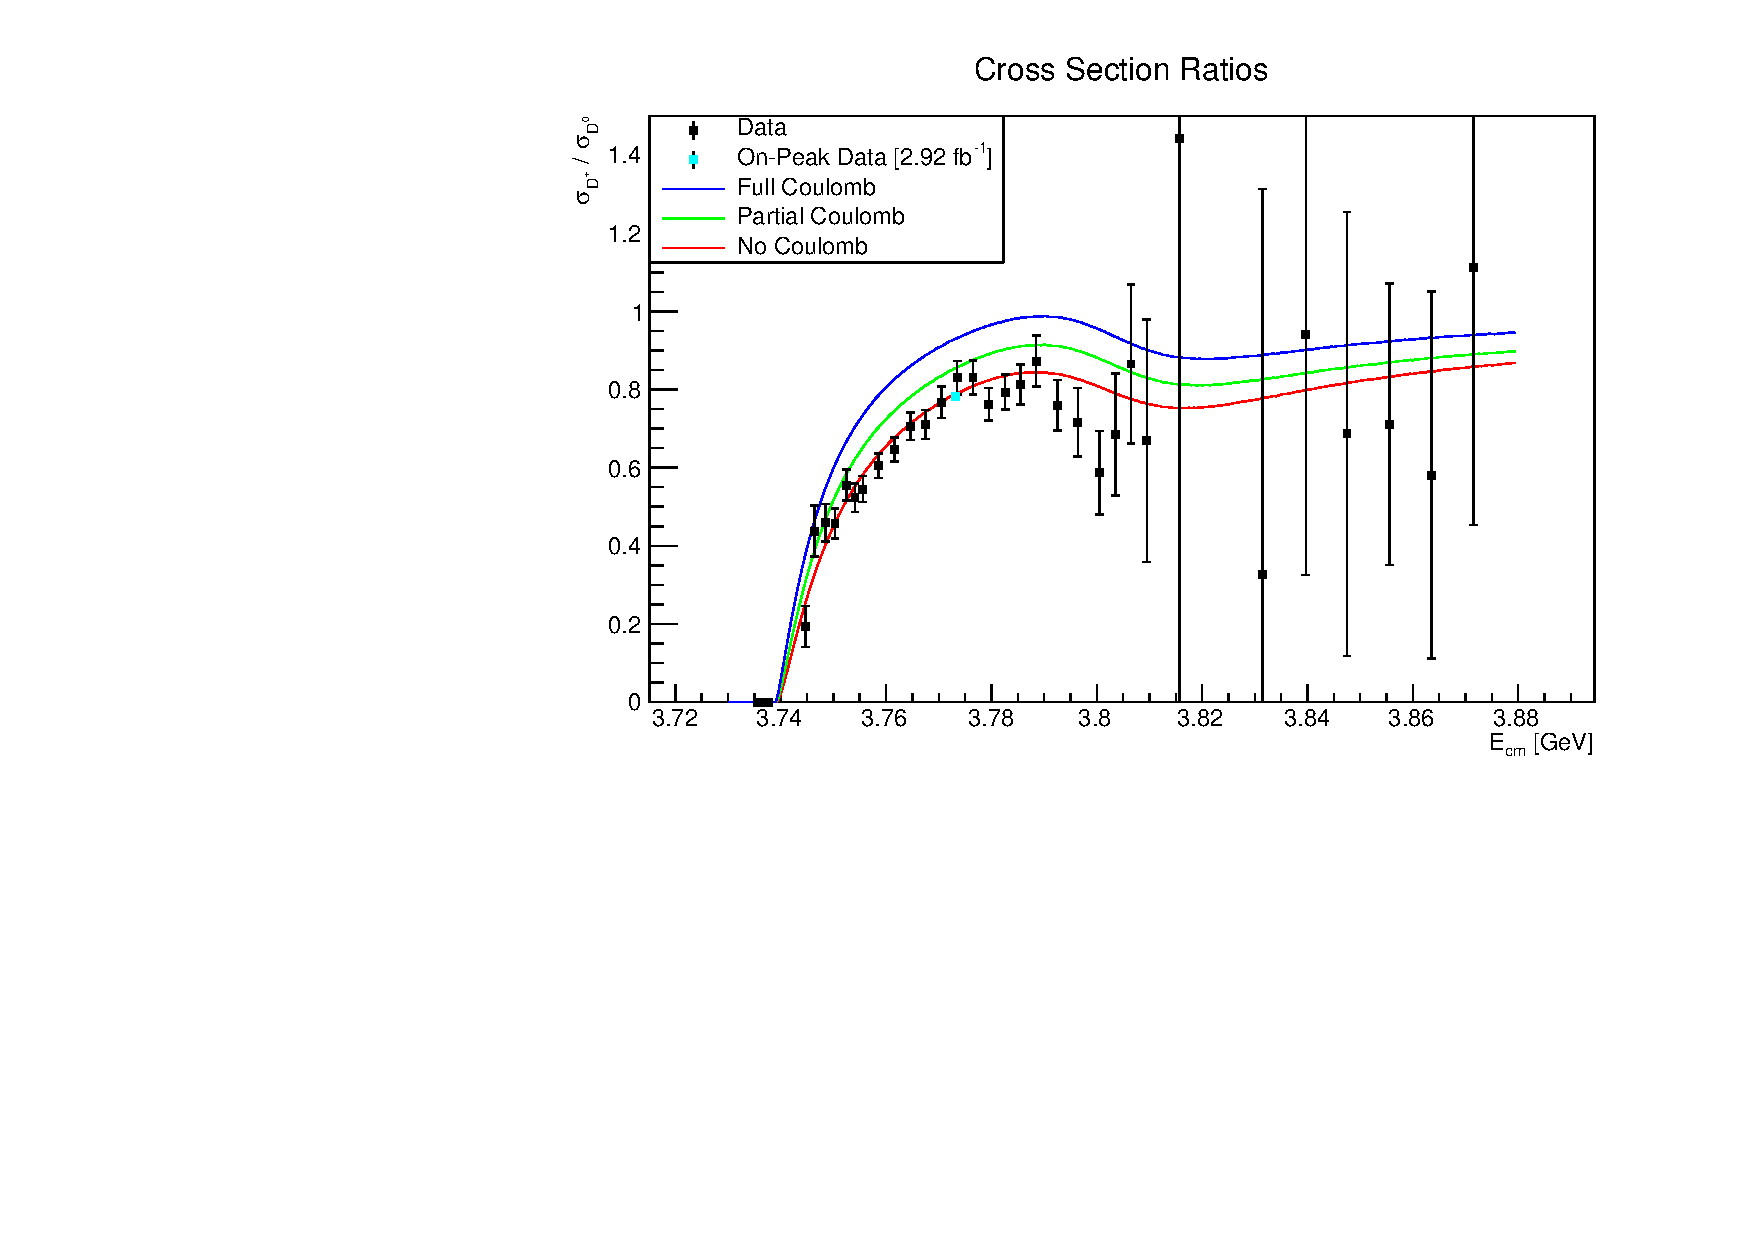
\includegraphics[scale=0.75]{figures/plots/Coulomb_ratio.pdf}
\caption{The ratio of $\Dp$ to $\DO$ cross sections.}
{Several levels of Coulomb interactions are examined.}
\label{fig:Coulomb_ratio}
\end{figure}


\section{Systematics}
\label{sec:systematics}

To assess the systematic uncertainties in our results, we look at a variety of factors.
Many of these affect all BESIII analyses, such as luminosity and tracking.
Others, like the modification to KKMC generation (see \Cref{ssec:monte_carlo}), are specific to this analysis.
The remaining systematics are typically due to less well-known parameters, like the radii used to describe the $\psip$ and $\psipp$ (see \Cref{sec:form_factors}).
Each of these contributions, as well as their total, can be found in \Cref{tab:systematics}. 

Each systematic is obtained by changing a specific aspect, and re-fitting to the altered values using the VDM method.
The uncertainties for each parameter are obtained by taking the difference between this result and the nominal fit (\Cref{fig:vdm_results}).
Generally, each change was done both positively and negatively, and the value used is the largest difference seen between the two changes.
The contributing systematics are summarized below:


\subsection*{Luminosity}
\label{ssec:sys_luminosity}

A \SI{1}{\%} change was applied to $\lum$ in \Cref{eq:xsec_rc_data}.


\subsection*{$\pipm / \Kpm$ Tracking}
\label{ssec:sys_Kpi_tracking}

A \SI{1.0}{\%} change was applied for each $\pipm$ or $\Kpm$ in a given decay mode.  
The summed contribution for each mode is applied to $\epsilon_m$ in \Cref{eq:DDbar_eff}.


\subsection*{$\piO$ Tracking}
\label{ssec:sys_pi0_tracking}

A \SI{2.0}{\%} change was applied for each $\piO$ in a given decay mode.
The summed contribution for each mode is applied to $\epsilon_m$ in \Cref{eq:DDbar_eff}.


\subsection*{$\Ks$ Tracking}
\label{ssec:sys_Ks_tracking}

A \SI{1.5}{\%} change was applied for each $\Ks$ in a given decay mode.
The summed contribution for each mode is applied to $\epsilon_m$ in \Cref{eq:DDbar_eff}.


\subsection*{Signal Shape}
\label{ssec:sys_signal_shape}

A mode-dependent change was applied to $N$ in \Cref{eq:xsec_rc_data}.
Differences in signal shapes were obtained by Derrick Toth after examining the use of single-Gaussian convolved signal shapes, and are shown in \Cref{tab:sys_signal_shape}. 
The changes applied were obtained from the sums of the mode-dependent values averaged over their branching fractions.


\begin{table}[H]
\centering
\renewcommand\arraystretch{1.0}
\begin{tabular}{l|c}
\hline
\multicolumn{1}{c|}{Tag Mode} & Difference (\%) \\
\hline
$\DOmodeA$ & 0.27 \\
$\DOmodeB$ & 0.10 \\
$\DOmodeC$ & 0.47 \\
\hline
\multicolumn{2}{c}{$\DO$ Average: \SI{0.24}{\%}} \\
\hline
$\DpmodeA$ & 0.20 \\
$\DpmodeB$ & 0.00 \\
$\DpmodeC$ & 0.17 \\
$\DpmodeD$ & 0.29 \\
$\DpmodeE$ & 0.17 \\
$\DpmodeF$ & 0.74 \\
\hline
\multicolumn{2}{c}{$\Dp$ Average: \SI{0.19}{\%}} \\
\hline
\end{tabular}
\caption{Signal shape differences by mode.}
{The total $\DO$ and $\Dp$ values are averaged over the branching fractions for each mode.}
\label{tab:sys_signal_shape}
\end{table}

In generating the MC samples for this analysis, several used a modified form of KKMC which accounted for the line shape of the $\psipp$.
However, as this shape is also the final output of the procedure, only an estimation of the results can be used for generation.
To assess the variation from the input shape, we compared the output fit parameters to those used in the generation process, and found very similar fit parameters.
This process used the Exponential method, and can be found in Table \ref{tab:KKMC_parameters}.
The numbers listed are from an earlier iteration of the MC than shown in Sec. \ref{sec:fitting}, but the consistency seen is representative of all iterations.
Very little difference is seen in the primary fitting parameters of the $\psipp$.
These similarities show the fit result values converging, even after only a single iteration.

\begin{table}[h!]
\begin{tabular}{c|cccccc}
\hline 
 & $\Mpsipp$ [GeV] & $\Gpsipp$ [MeV] & $\GeepsipptoDD$ [eV] & $\Ppsipp$ & $\Gpsip$ [MeV] & $F_{0}$ \\ 
\hline 
Fit Results & 3.7814 $\pm$ 0.0003~& 24.839 $\pm$ 0.681~& 214.65 $\pm$ 11.10~& 3.6375 $\pm$ 0.0518~& 20.147 $\pm$ 1.765~& -1.5265 $\pm$ 0.5119 \\ 
KKMC Input & 3.7815 $\pm$ 0.0003~& 24.887 $\pm$ 0.686~& 217.55 $\pm$ 11.18~& 3.6374 $\pm$ 0.0513~& 21.394 $\pm$ 1.866~& -1.6202 $\pm$ 0.5271 \\ 
\hline
\end{tabular} 
\caption{The parameters used to modify the KKMC lineshape of the $\psipp$ compared to the Exponential fit results.}
\label{tab:KKMC_parameters}
\end{table}

We also considered an alternative MC simulation of the $\DDbar$ samples based on the ConExc generator in place of KKMC.
This process used an input Born level shape identical to that used in the final iteration produced with KKMC.
Each of the background samples used (such as $\qqbar$ and $\tautau$) were the same as in the nominal procedure.
The cross section results using the VDM model are shown in Fig. \ref{fig:ConExc}, and provide $\psipp$ fit parameters within the statistical errors of the nominal method, as seen in Fig. \ref{fig:vdm_results}.
From this, we treat variations due to the MC generation as negligible.

\begin{figure}
\centering
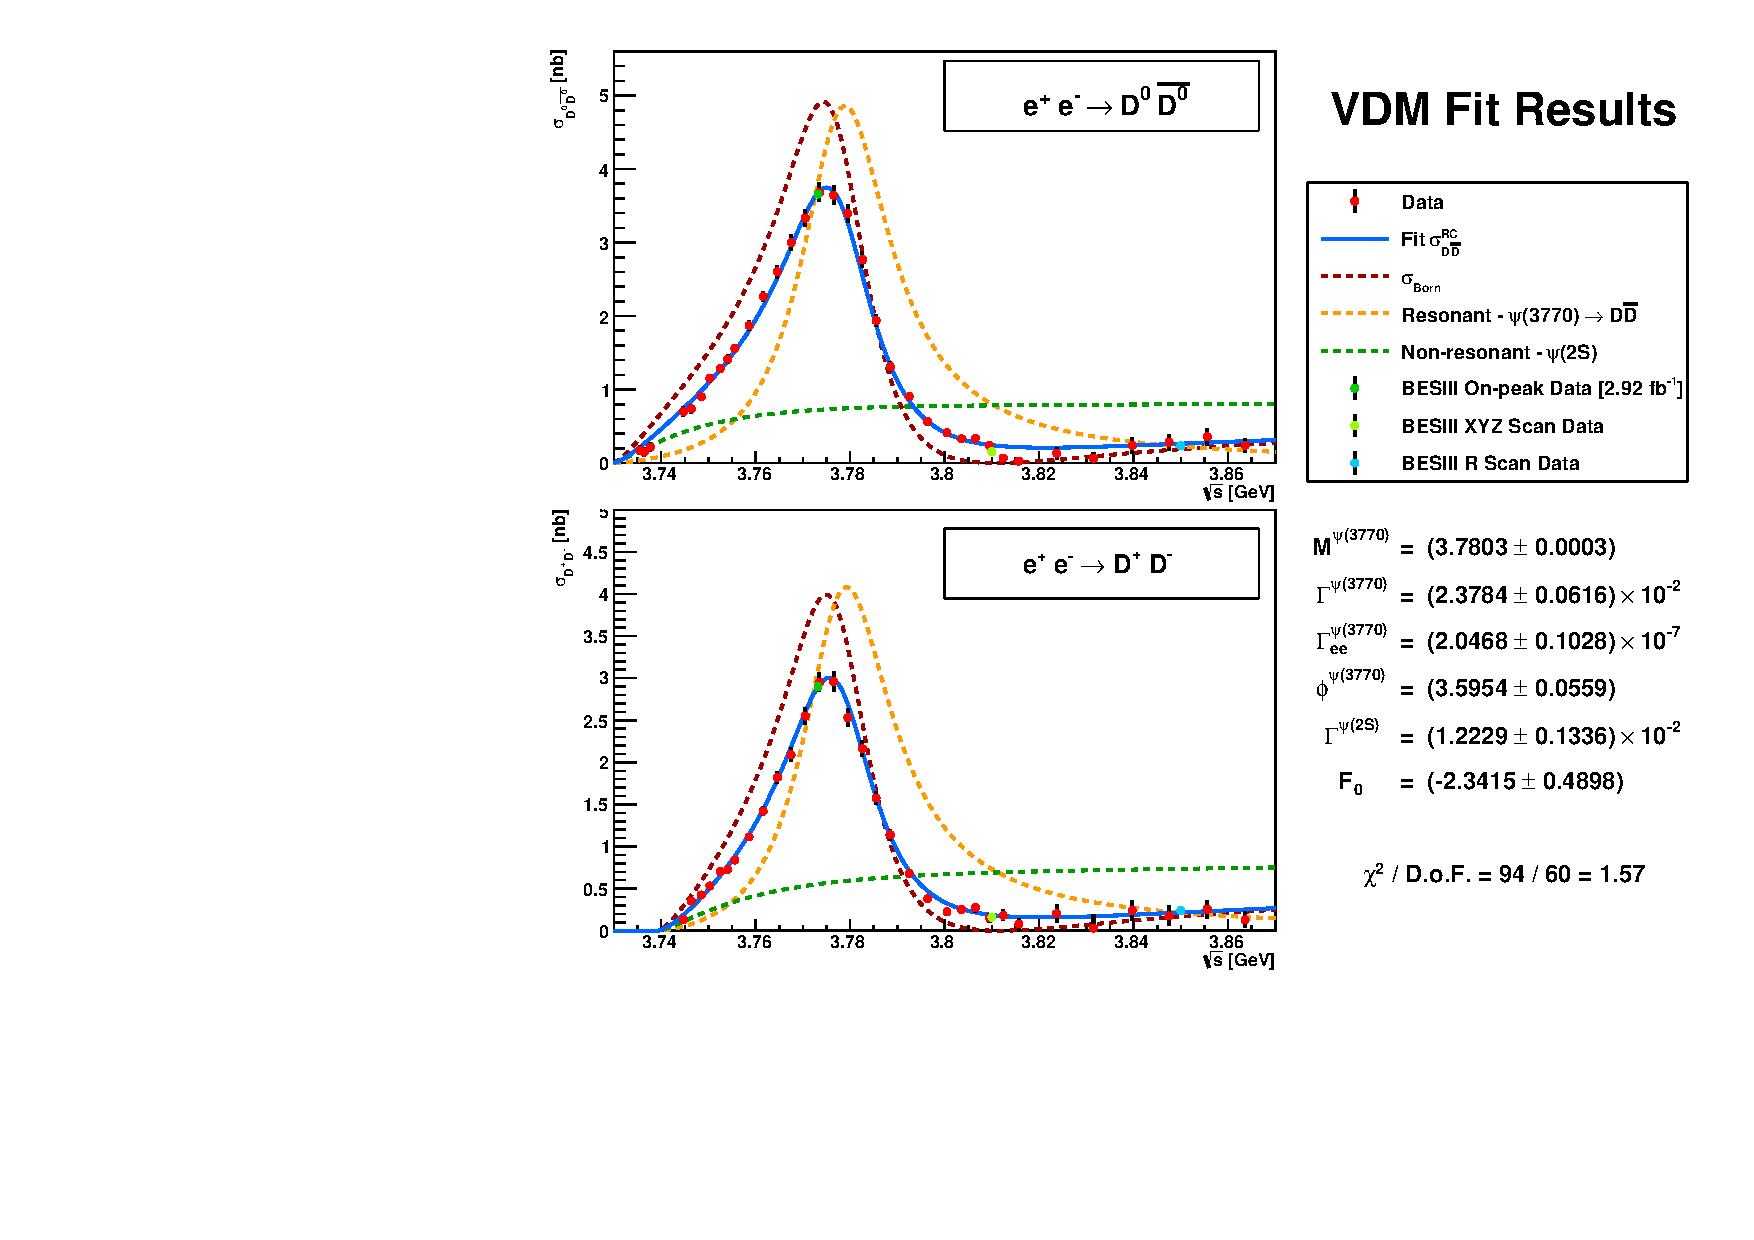
\includegraphics[scale=0.45]{figures/plots/lineshape_vdm_ConExc.pdf}
\caption{The Vector Dominance Model fit results for (left) $\DO$ and (right) $\Dp$.  The underlying MC shapes for the $\DDbar$ components were generated using ConExc instead of KKMC.}
\label{fig:ConExc}
\end{figure}



\section{Results}
\label{sec:results}



\chapter{Measurement of Hadronic Production and $\Gamma(\psipp \rightarrow \nonDDbar)$}
\label{ch:non_DDbar}

The second part of the analysis concerns the measurement of hadronic events over the scan data energy region.
Using this information, we can extract the number of $\nonDDbar$ events found in data by subtracting all other known decay processes.
Comparing the found production rate of $\nonDDbar$ events to the previous measurement of $\xsecpsipptoDDbar$, we can then analyze the branching fraction of $\Gamma(\psipp \rightarrow \nonDDbar)$.


In order to determine the amount of hadronic events in the scan data region, we use continuum data taken at a lower energy (around \SI{3.650}{\GeV}).
This is due to complicated interactions in the region above the $\DDbar$ threshold which are currently not well modeled by our MC generators.
However, below the $\psip$, the process is more reliable.
If the production of hadronic events remains consistent over energy, we can use these measurements at lower energies to extract values at higher energies.

\section{Data and Monte Carlo Samples}
\label{sec:non_DDbar_data_samples}

\subsection{Data Samples}
\label{ssec:data_samples_non_DDbar}

The data used for this analysis was also produced by BEPCII and collected by BESIII.
The samples used include continuum data taken at \SI{3.650}{\GeV} in 2009 (old continuum), as well as multiple other continuum points taken around this energy in 2013 (new continuum).
We also use Round 1 (R1) and Round 2 (R2) of the high-statistics $\psipp$ data taken in 2010 and 2011, respectively.
Each of these samples, and their measured luminosities, can be seen in \Cref{tab:data_samples_non_DDbar}.
The values of luminosity were measured during a previous version of this analysis using the procedure described in \Cref{ssec:luminosity_measurement}.
The labels given to each continuum point are the intended energy targets, but may differ from their true values.
In addition to these datasets, the scan data described previously (\Cref{ssec:data_samples}) is also used.


\subsection{Center-of-Mass Energy Measurement}
\label{ssec:energy_measurement_non_DDbar}

As before, a precise measurement of each energy point is vital to the accuracy of the final results.
Most notably, due to the rapidly increasing shape of the $\psip$ cross section near the high end of the continuum points, the value of the 3671 (New) point has a dramatic effect on the $\qqbar$ extrapolation.
Following the procedure of \Cref{ssec:energy_measurement}, we measured the $\Ecm$ value of each continuum point.
This resulted in a \SIrange{4}{6}{\MeV} shift downwards for each of the new continuum points, but virtually no shift for the old continuum point.
The energy measurements are shown in \Cref{tab:data_samples_non_DDbar}.


\begin{table}[H]
\centering
\renewcommand\arraystretch{1.0}
\begin{tabular}{l|c r}
\hline
Sample Name & $\Ecm$ [\si{\GeV}] & Luminosity \si{\invpb} \\
\hline
3500 (New) & 3.496 & \num{  3.680 \pm 0.009} \\
3542 (New) & 3.538 & \num{  3.481 \pm 0.009} \\
3600 (New) & 3.596 & \num{  0.395 \pm 0.019} \\
3650 (New) & 3.644 & \num{  5.420 \pm 0.009} \\
3671 (New) & 3.665 & \num{  4.669 \pm 0.009} \\
3650 (Old) & 3.650 & \num{ 44.334 \pm 0.009} \\
3773 (R1)  & 3.773 & \num{926.922 \pm 0.092} \\
3773 (R2)  & 3.773 & \num{1978.92 \pm 0.091} \\
\hline
\end{tabular}
\caption{Data samples used for the inclusive measurement.}
{While the 3600 (New) sample was intended to be similar in luminosity to the other continuum points, accelerator issues inhibited the data collection procedure. 
The new continuum points also have a much smaller luminosity compared to the other datasets used in this analysis.}
\label{tab:data_samples_non_DDbar}
\end{table}


\section{Event Selection}
\label{sec:non_DDbar_event_selection}

In order to select the number of hadronic events in each sample, we apply a variety of cuts.
For charged tracks in the MDC, these include the cuts shown in \Cref{tab:charged_cuts_non_DDbar}.

\begin{table}[H]
\centering
\renewcommand\arraystretch{1.0}
\begin{tabular}{c| r@{$\; < \;$}l}
\hline
Vertex ($xy$) & $V_{xy}$ & \pp \SI{1}{\cm} \\
Vertex ($z$)  & $|Vz|$   & \SI{10}{\cm} \\
MDC Angle & $|\cos\theta|$ & 0.93 \\
\hline
\end{tabular}
\caption{Selection cuts on charged tracks used to count hadronic events.}
\label{tab:charged_cuts_non_DDbar}
\end{table}

For neutral tracks in the EMC, these include the cuts shown in \Cref{tab:neutral_cuts_non_DDbar}.

\begin{table}[H]
\centering
\renewcommand\arraystretch{1.0}
\begin{tabular}{c|l r}
\hline
Minimum Energy (Barrel) & $E_{\text{EMC}} > \SI{25}{\MeV}$ & $(|\cos\theta| < 0.80)$ \\
Minimum Energy (Endcap) & $E_{\text{EMC}} > \SI{50}{\MeV}$ & $(0.86 < |\cos\theta| < 0.92)$ \\
TDC Timing & $(0 \leq t \leq 14) \times \SI{50}{\ns}$ & \\
\hline
\end{tabular}
\caption{Selection cuts on neutral tracks used to count hadronic events.}
\label{tab:neutral_cuts_non_DDbar}
\end{table}


To reject background events of $\bhabha$ or $\ee \rightarrow \gamma\gamma$, we also employ cuts related to the most energetic and highest momentum tracks in the event.
These are listed in \Cref{tab:bhabha_cuts_non_DDbar}.

\begin{table}[H]
\centering
\renewcommand\arraystretch{1.0}
\begin{tabular}{l|l@{}l l@{}l}
\hline
\multirow{4}{*}{Highest Energy}   & $\cosmax_+ <  $ & 0.8                            & \multirow{2}{*}{($\Ntrk$} & \multirow{2}{*}{ = 2)} \\
                                  & $\cosmax_- > -$ & 0.8                            & & \\
\cline{2-5}
                                  & $\cosmax_+ <  $ & 0.8 or $\pEmax_+ \leq 0.3$     & \multirow{2}{*}{($\Ntrk$} & \multirow{2}{*}{ = 3, 4)} \\
                                  & $\cosmax_- > -$ & 0.8 or $\pEmax_- \leq 0.3$     & & \\
\hline
\multirow{2}{*}{Highest Momentum} & \multicolumn{2}{l}{$0.8 \leq \Epmax_+ \leq 1.1$} & & \\
                                  & \multicolumn{2}{l}{$0.8 \leq \Epmax_- \leq 1.1$} & & \\
\hline
\end{tabular}
\caption{Selection cuts to remove Bhabha and two-photon backgrounds.}
{The $_+$ and $_-$ denote positively and negatively charged tracks, respectively.  The $^{\text{max}}$ notation indicates the highest energy or momenta track for the corresponding charge.  The energy cuts depend on the total number of charged tracks in the event, $\Ntrk$.}
\label{tab:bhabha_cuts_non_DDbar}
\end{table}

After applying these sets of cuts, there are three groups of cuts which are considered: Standard (SHAD), Loose (LHAD), and Tight (THAD).
For the nominal procedure, SHAD is used, while LHAD and THAD are for systematic consideration.
The cuts included in each of these sets are shown in \Cref{tab:shad_cuts_non_DDbar,tab:lhad_cuts_non_DDbar,tab:thad_cuts_non_DDbar}.
These apply to the number of charged tracks ($\Ntrk$), the visible energy ($\Evis$), the total visible momentum in the $z$-direction ($\pzvistot$), the maximum shower energy ($\Eemcmax$), and the total shower energy ($\Eemctot$).
Here, `visible' refers to the sum over charged and neutral tracks.

\begin{table}[H]
\centering
\renewcommand\arraystretch{1.0}
\begin{tabular}{l|r@{ }l l}
\hline
Number of Tracks                     & $\Ntrk$ & $ > 2$               &                  \\
\hline
Visible Energy                       & $\EvisE$ & $ > 0.3$            &                  \\
\hline
Visible Momentum                     & $\pzEvis$ & $ < 0.6$           & $(\Ntrk = 3, 4)$ \\
\hline
Maximum Shower Energy                & $\EemcEmax$ & $ < 0.75$           & $(\Ntrk = 3, 4)$ \\
\hline
\multirow{2}{*}{Total Shower Energy} & \multicolumn{2}{c}{$0.25 < \EemcEtot < 0.75$} & $(\Ntrk = 3)$ \\
                                     & \multicolumn{2}{c}{$0.15 < \EemcEtot < 0.75$} & $(\Ntrk = 4)$ \\
\hline
\end{tabular}
\caption{Standard selection cuts (SHAD) for counting hadronic events.}
\label{tab:shad_cuts_non_DDbar}
\end{table}

\begin{table}[H]
\centering
\renewcommand\arraystretch{1.0}
\begin{tabular}{l|r@{ }l l}
\hline
Number of Tracks                       & $\Ntrk$ & $ > 1$               &                  \\
\hline
\multirow{2}{*}{Visible Energy}        & $\EvisE$ & $ > 0.4$            & $(\Ntrk = 2)$    \\
                                       & $\EvisE$ & $ > 0.3$            & $(\Ntrk \geq 3)$ \\
\hline                                 
\multirow{2}{*}{Visible Momentum}      & $\pzEvis$ & $ < 0.3$           & $(\Ntrk = 2)$    \\
                                       & $\pzEvis$ & $ < 0.6$           & $(\Ntrk = 3, 4)$ \\
\hline
\multirow{2}{*}{Maximum Shower Energy} & $\EemcEmax$ & $ < 0.50$           & $(\Ntrk = 2)$    \\
                                       & $\EemcEmax$ & $ < 0.75$           & $(\Ntrk = 3, 4)$ \\
\hline                                 
\multirow{2}{*}{Total Shower Energy}   & \multicolumn{2}{c}{$0.25 < \EemcEtot < 0.75$} & $(\Ntrk = 2, 3)$ \\
                                       & \multicolumn{2}{c}{$0.15 < \EemcEtot < 0.75$} & $(\Ntrk = 4)$    \\
\hline
\end{tabular}
\caption{Loose selection cuts (LHAD) for counting hadronic events.}
\label{tab:lhad_cuts_non_DDbar}
\end{table}

\begin{table}[H]
\centering
\renewcommand\arraystretch{1.0}
\begin{tabular}{l|r@{ }l l}
\hline
Number of Tracks                     & $\Ntrk$ & $ > 3$               &                  \\
\hline
Visible Energy                       & $\EvisE$ & $ > 0.4$            &                  \\
\hline
Visible Momentum                     & $\pzEvis$ & $ < 0.6$           & $(\Ntrk = 4)$ \\
\hline
Maximum Shower Energy                & $\EemcEmax$ & $ < 0.75$           & $(\Ntrk = 4, 5)$ \\
\hline
\multirow{2}{*}{Total Shower Energy} & \multicolumn{2}{c}{$0.15 < \EemcEtot < 0.75$} & $(\Ntrk = 4)$ \\
                                     & \multicolumn{2}{c}{$0.00 < \EemcEtot < 0.75$} & $(\Ntrk = 5)$ \\
\hline
\end{tabular}
\caption{Tight selection cuts (THAD) for counting hadronic events.}
\label{tab:thad_cuts_non_DDbar}
\end{table}

\section{Hadron Counting}
\label{sec:hadron_counting}

In order to determine the total number of hadronic events in each data sample, we use the average velocity in the $z$-direction.
Signal events should have tracks which average to zero around the collision point, while background events will have randomly oriented momenta.
The fits are done with a double Gaussian shape for the signal and a 2nd order polynomial for the background.

\begin{figure}[H]
\centering
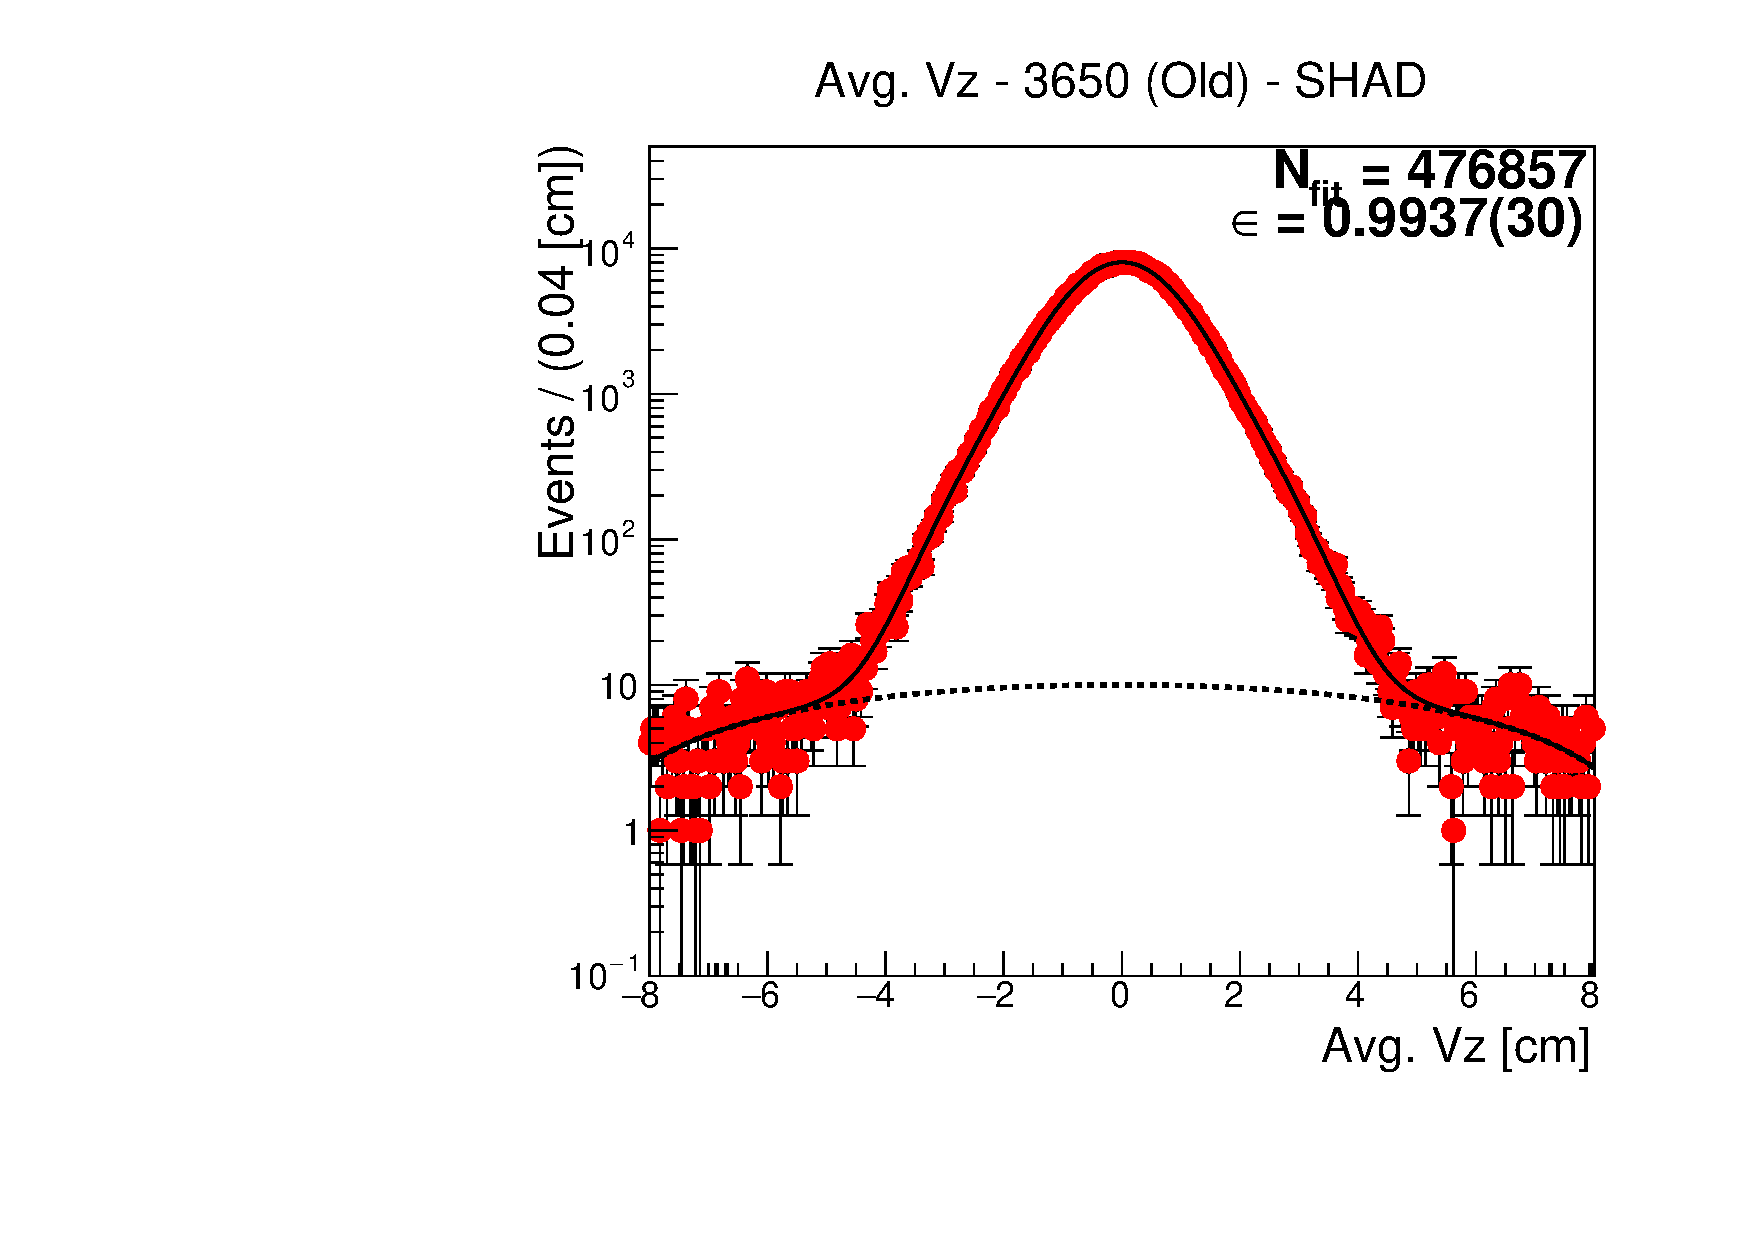
\includegraphics[scale=0.25]{figures/plots/nonDDbar_fit_results/3650_old/fit_old_3650_data_SHAD.pdf}
\hspace{-0.5cm}
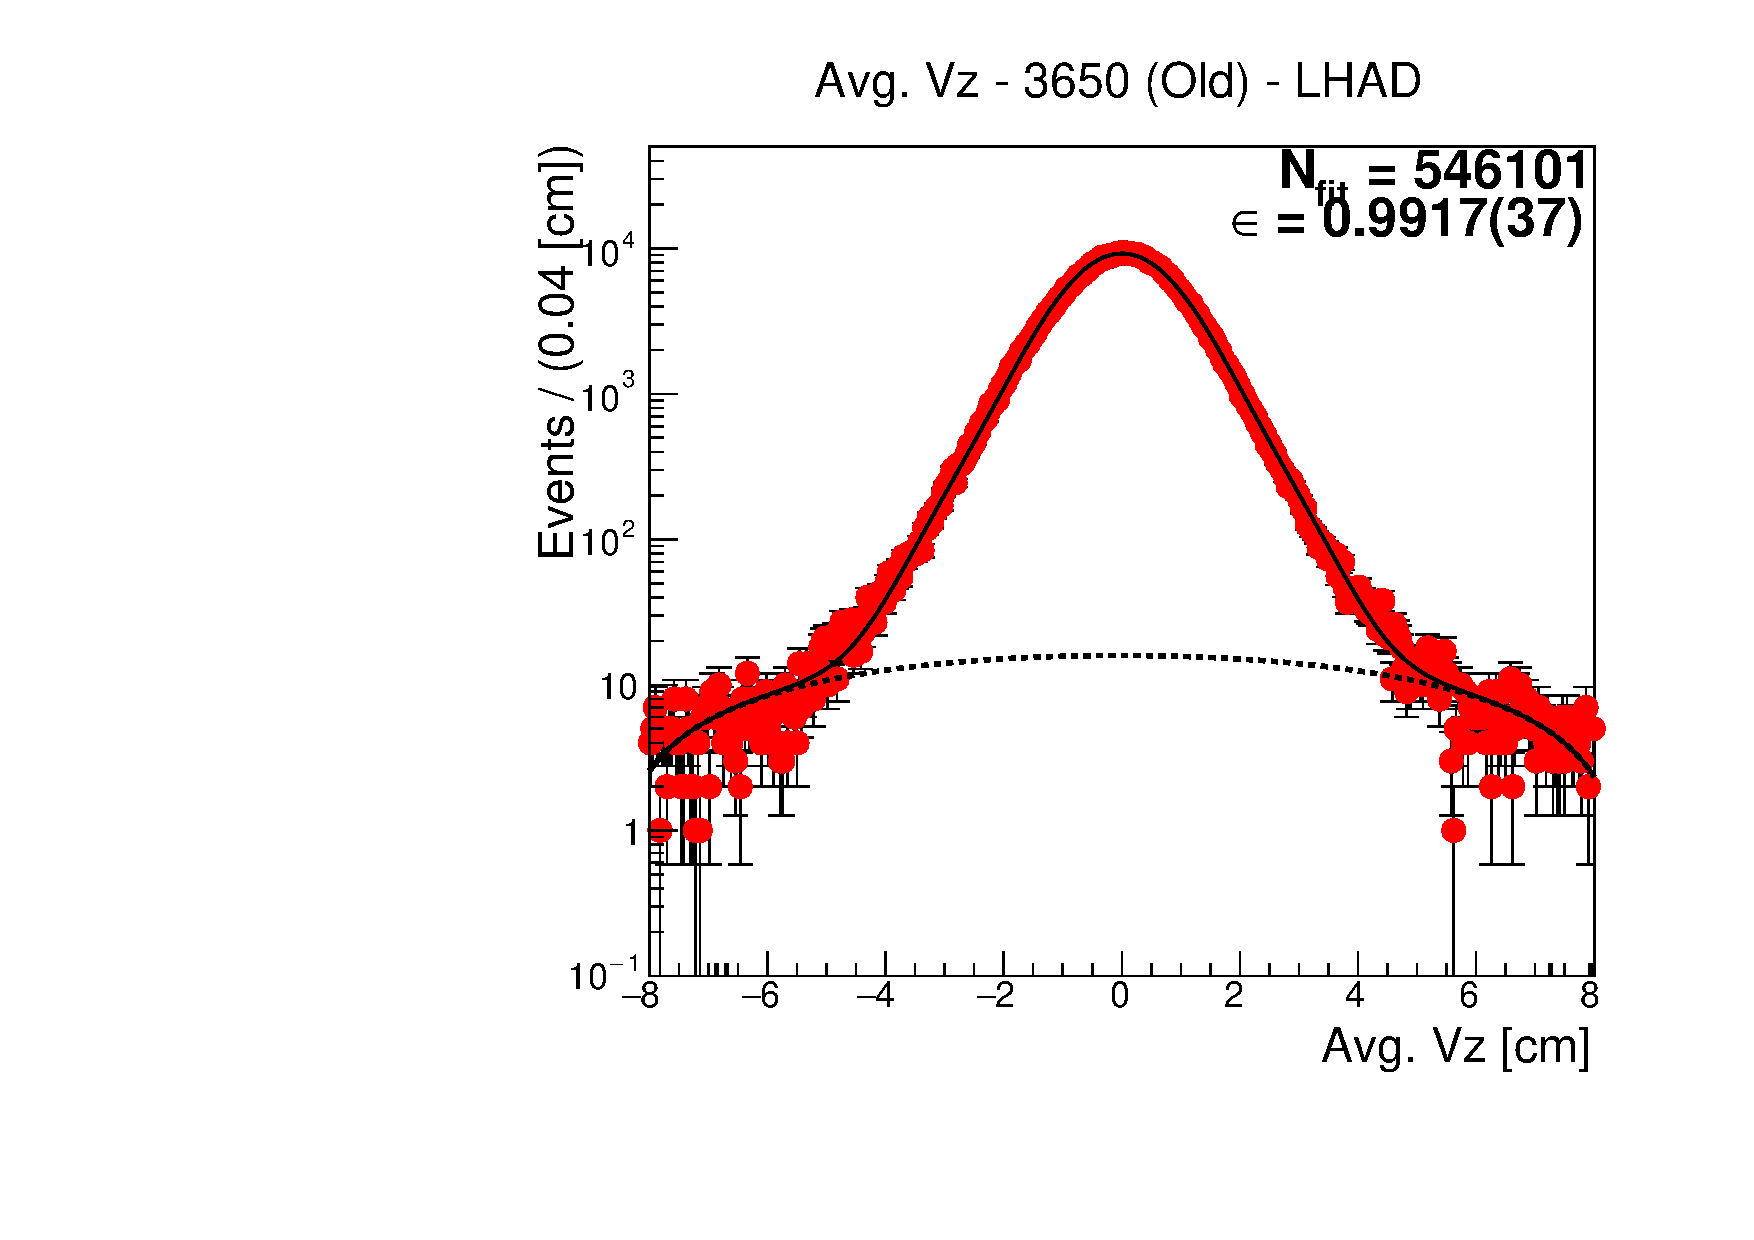
\includegraphics[scale=0.25]{figures/plots/nonDDbar_fit_results/3650_old/fit_old_3650_data_LHAD.pdf}
\hspace{-0.5cm}
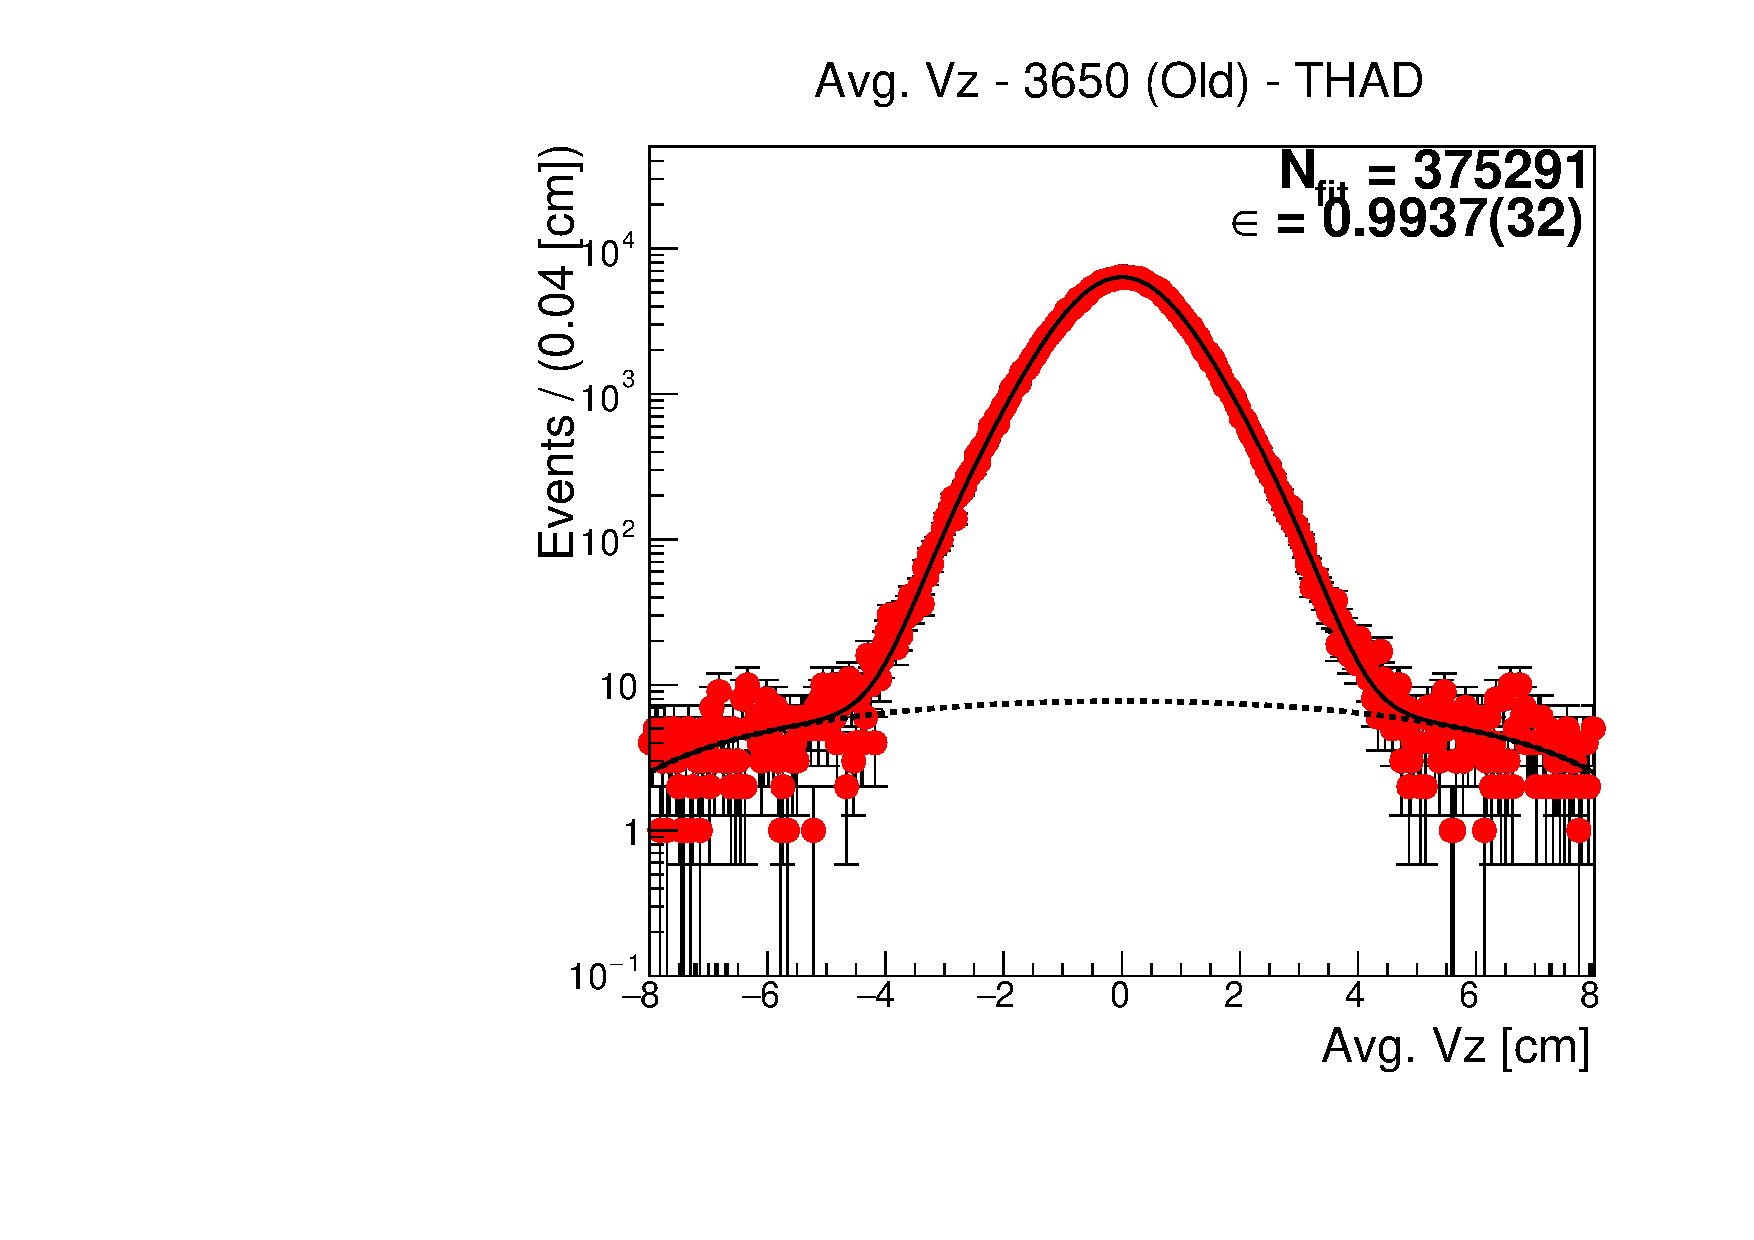
\includegraphics[scale=0.25]{figures/plots/nonDDbar_fit_results/3650_old/fit_old_3650_data_THAD.pdf}
\caption{The number of hadrons found in the 3650 (Old) data sample.}
{This includes results for SHAD (left), LHAD (middle), and THAD (right).}
\label{fig:hadron_fits_3650_old}
\end{figure}


\section{Background Subtraction}
\label{sec:background_subtraction}

To precisely determine the number of hadronic events in the old continuum sample, we must subtract off a variety of backgrounds.
The samples considered for this measurement include two-track QED processes ($\ee$, $\mumu$, $\tautau$, $\yy$), radiative $\jpsi$ ($\yjpsi$), two photon fusion ($\twophoton$), and events coming from $\psip$.
Initially, we assume the $\psip$ has a standard Breit-Wigner shape.

Each background contributes to the total number of reconstructed events based on their cross section ($\sigma$) and reconstruction efficiency ($\effmc$):
\beq
\Nhad = \lum \times \sigma \times \effmc.
\eeq
The efficiency is simply the fraction of reconstructed tracks of the total generated in a given MC sample:
\beq
\effmc = \left( \frac{ N_{\text{rec}} }{ N_{\text{gen}} } \right)
\eeq
The MC samples were generated with \num{2.5e3} events for each of the 79 runs in the old continuum data for each of the included backgrounds.
Each sample was analyzed with all three cut selection groups (see \Cref{sec:non_DDbar_event_selection}).
The reconstruction efficiencies for each, along with their cross sections at \SI{3.650}{\GeV} are shown in \Cref{tab:3650_old_reconstruction}.

\begin{table}[H]
\centering
\renewcommand\arraystretch{1.0}
\begin{tabular}{c|r|cr@{$\; \pm \;$}rc cr@{$\; \pm \;$}rc cr@{$\; \pm \;$}rc}
\hline
\multicolumn{14}{c}{3650 (Old) Reconstruction} \\
\hline
Sample & $\sigma$ [\si{\pb}] & \multicolumn{4}{c}{$\effmc$ (SHAD) [\%]} & \multicolumn{4}{c}{$\effmc$ (LHAD) [\%]} & \multicolumn{4}{c}{$\effmc$ (THAD) [\%]} \\
\hline
$\ee$           & 554.562 &&  0.0006 & 0.0002 &&&  0.0008 & 0.0002 &&&  0.0001 & 0.0001 & \\
$\mumu$         &   5.560 &&  0.0033 & 0.0004 &&&  0.0044 & 0.0005 &&&  0.0029 & 0.0004 & \\
$\tautau$       &   1.844 && 12.8351 & 0.0255 &&& 28.7692 & 0.0382 &&&  9.9371 & 0.0224 & \\
$\yjpsi$        &   1.260 && 45.9222 & 0.0482 &&& 55.1722 & 0.0529 &&& 34.1250 & 0.0416 & \\
$\yy$           &  21.530 &&  0.0009 & 0.0002 &&&  0.0010 & 0.0002 &&&  0.0005 & 0.0002 & \\
$\twophoton$    &   1.257 &&  2.4109 & 0.0110 &&&  4.6297 & 0.0153 &&&  1.6468 & 0.0091 & \\
$\psip^\dagger$ &   0.150 && 62.9891 & 0.0078 &&& 69.2882 & 0.0082 &&& 51.6942 & 0.0071 & \\
\hline
\end{tabular}
\caption{Reconstruction of background samples for the old continuum data.}
{These include standard QED two-track processes ($\ee$, $\mumu$, $\tautau$, $\gamma\gamma$), radiative $\jpsi$ ($\gamma\jpsi$) and two photon fusion ($2\gamma$) events, and a contribution coming from $\psip$. \\
$^\dagger$ The $\psip$ is assumed to have a standard Breit-Wigner shape.}
\label{tab:3650_old_reconstruction}
\end{table}

Using each of these values, we can determine the total number of hadronic events in the data.
This is done by subtracting the expected amount of background from the measured number of events passing each selection method in data.
The results for the old continuum data are shown in \Cref{tab:3650_old_results}.

\begin{table}[H]
\centering
\renewcommand\arraystretch{1.0}
\begin{tabular}{c|cr@{$\; \pm \;$}rc cr@{$\; \pm \;$}rc cr@{$\; \pm \;$}rc}
\hline
\multicolumn{13}{c}{3650 (Old) Results} \\
\hline
Sample         & \multicolumn{4}{c}{$\Nhad$ (SHAD)} & \multicolumn{4}{c}{$\Nhad$ (LHAD)} & \multicolumn{4}{c}{$\Nhad$ (THAD)} \\
\hline
Data            && 477001 & 691 &&& 546546 & 739 &&& 375380 & 613 & \\
$\ee$           &&    149 &  43 &&&    187 &  48 &&&     12 &  12 & \\
$\mumu$         &&      8 &   1 &&&     11 &   1 &&&      7 &   1 & \\
$\tautau$       &&  10490 &  30 &&&  23514 &  59 &&&   8122 &  25 & \\
$\yjpsi$        &&  25658 &  60 &&&  30826 &  71 &&&  19067 &  46 & \\
$\yy$           &&      9 &   2 &&&     10 &   2 &&&      4 &   1 & \\
$\twophoton$    &&   1443 &   7 &&&   2771 &  11 &&&    986 &   6 & \\
$\psip^\dagger$ &&   1645 &   9 &&&   1810 &  10 &&&   1350 &   7 & \\
\hline                                                              
Total           && 437607 & 695 &&& 487428 & 747 &&& 345836 & 615 & \\
\hline
\end{tabular}
\caption{Hadronic events selected in the old continuum data.}
{As expected, SHAD finds more events than THAD and less than LHAD. \\
$^\dagger$ The $\psip$ is assumed to have a standard Breit-Wigner shape.}
\label{tab:3650_old_results}
\end{table}

Given that the $\ee$, $\mumu$, and $\yy$ samples have contributions which are much smaller than the uncertainty on the total result, we exclude these from future calculations.


\section{Efficiency Extrapolation}
\label{sec:efficiency_extrapolation}

To determine the number of hadronic events at each scan data point, we must first measure the hadronic production at each of the new continuum points.
This gives us a function of reconstruction efficiency over energy which we can use to extrapolate to the scan data region.
The process follows exactly as for the old continuum data, but with the negligible backgrounds excluded.
The number of hadrons found in each data sample can be seen in \Cref{fig:hadron_fits_3500_new,fig:hadron_fits_3542_new,fig:hadron_fits_3600_new,fig:hadron_fits_3650_new,fig:hadron_fits_3671_new}.
Reconstruction efficiencies for each of the new continuum points are shown in \Cref{tab:3650_new_reconstruction} with the total results shown in \Cref{tab:3650_new_results}.


\begin{figure}[H]
\centering
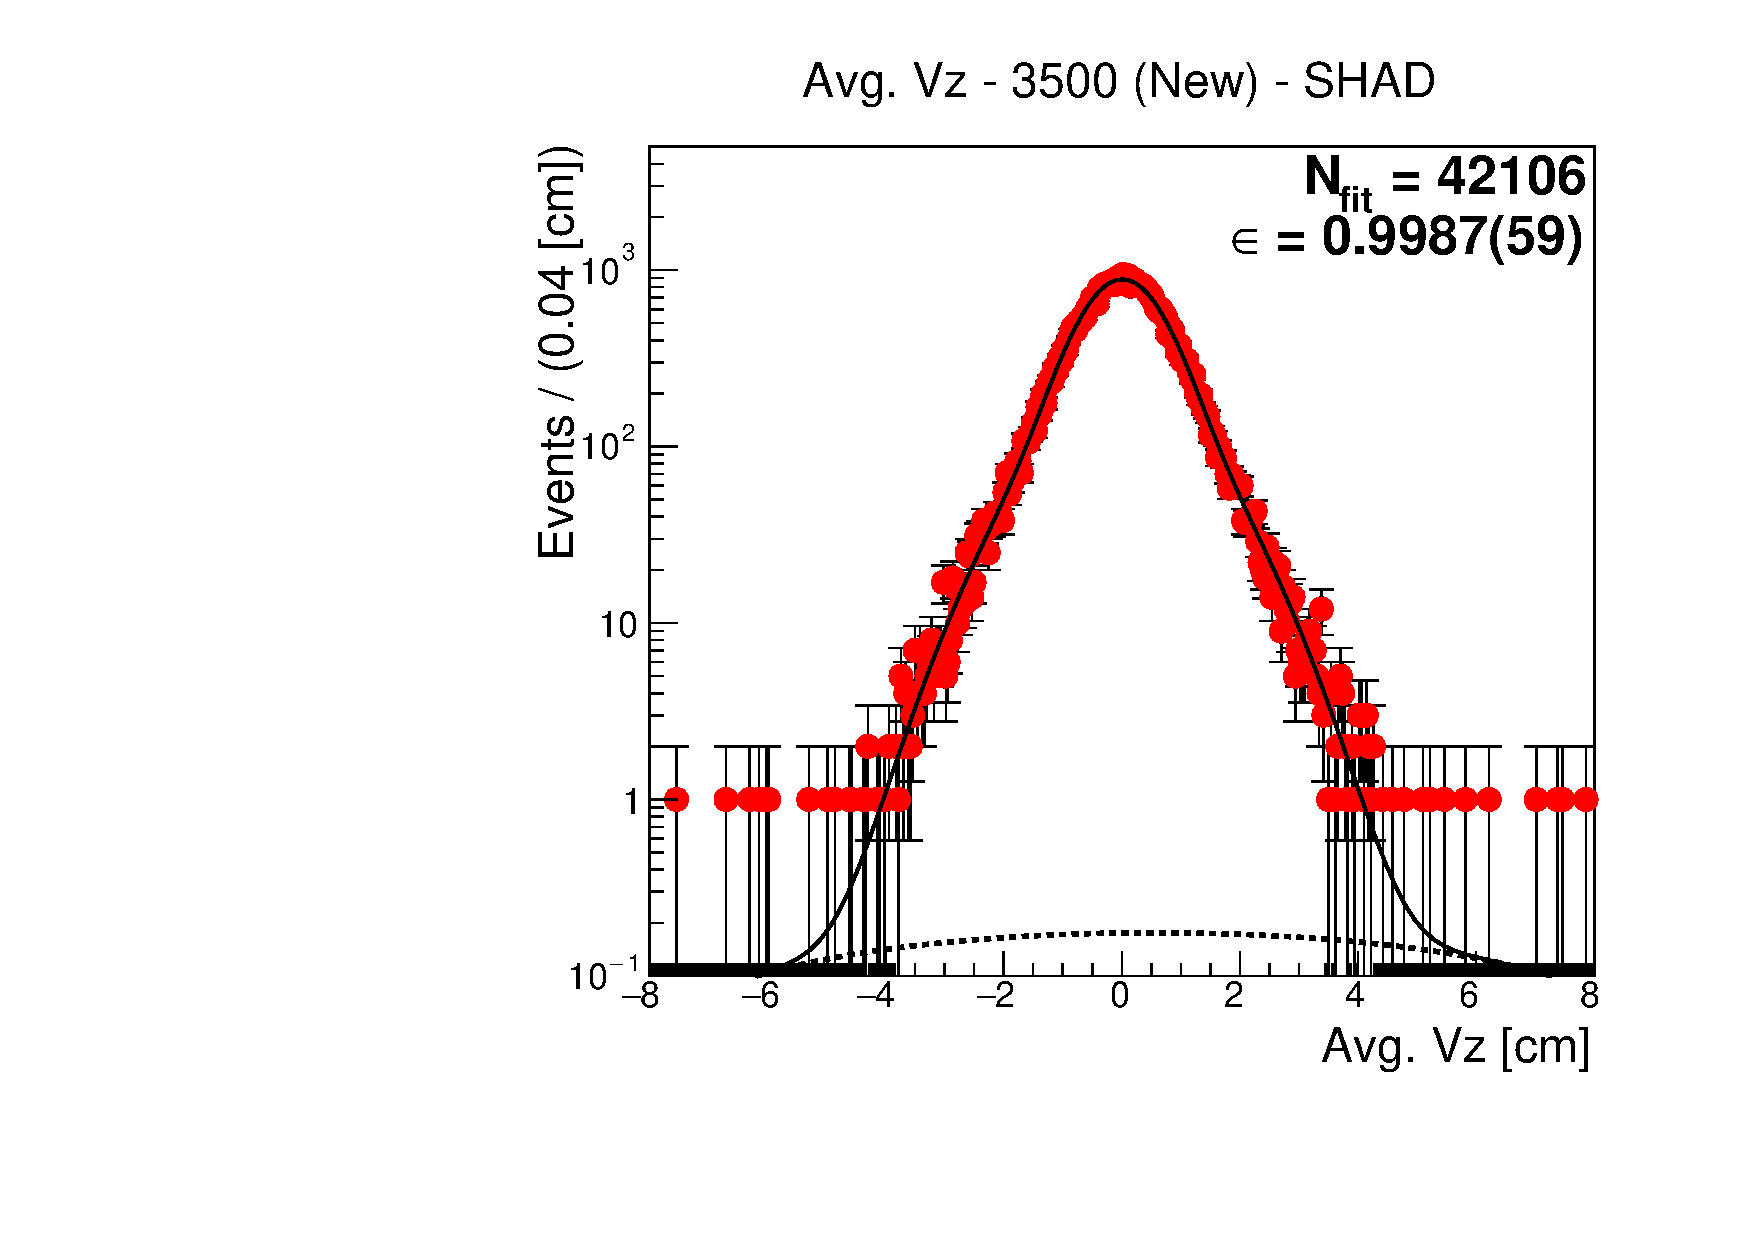
\includegraphics[scale=0.25]{figures/plots/nonDDbar_fit_results/3650_new/fit_new_3500_data_SHAD.pdf}
\hspace{-0.5cm}
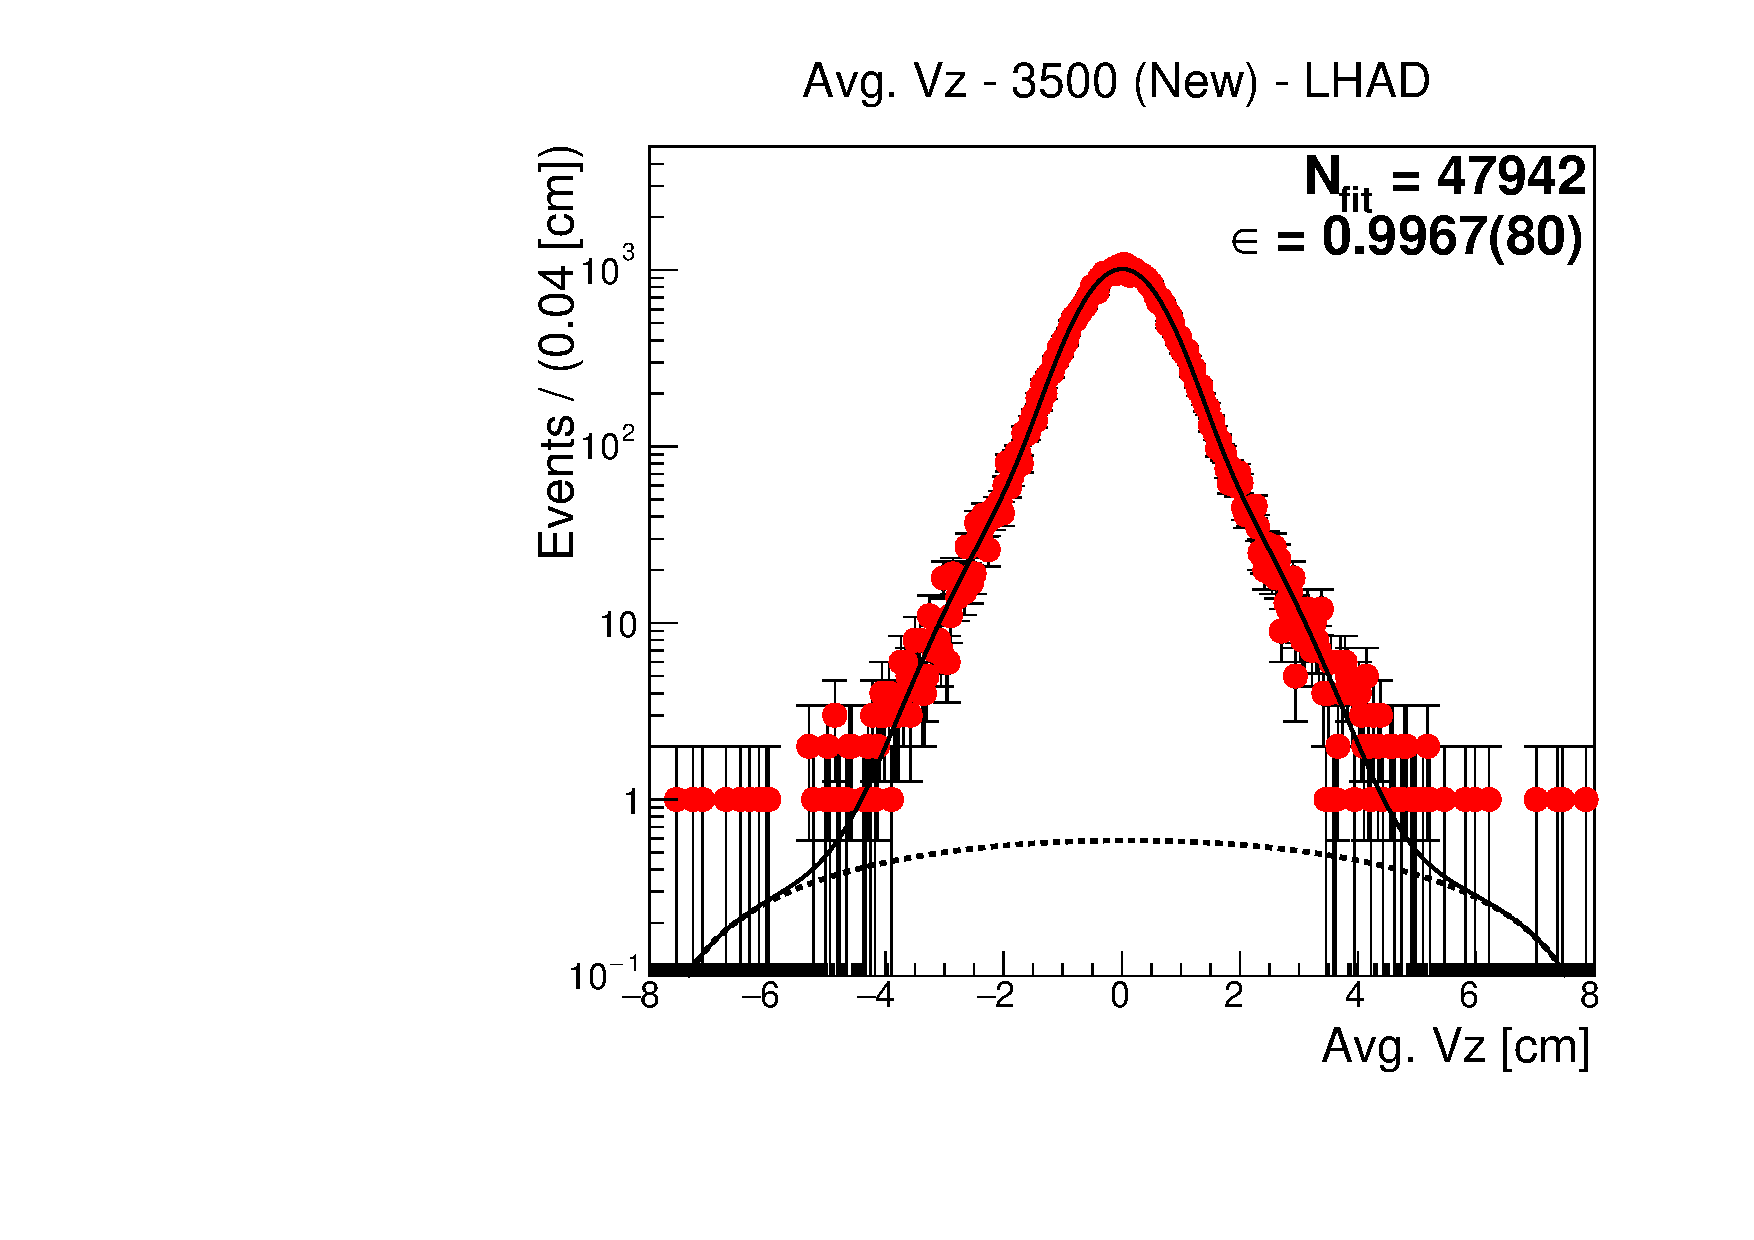
\includegraphics[scale=0.25]{figures/plots/nonDDbar_fit_results/3650_new/fit_new_3500_data_LHAD.pdf}
\hspace{-0.5cm}
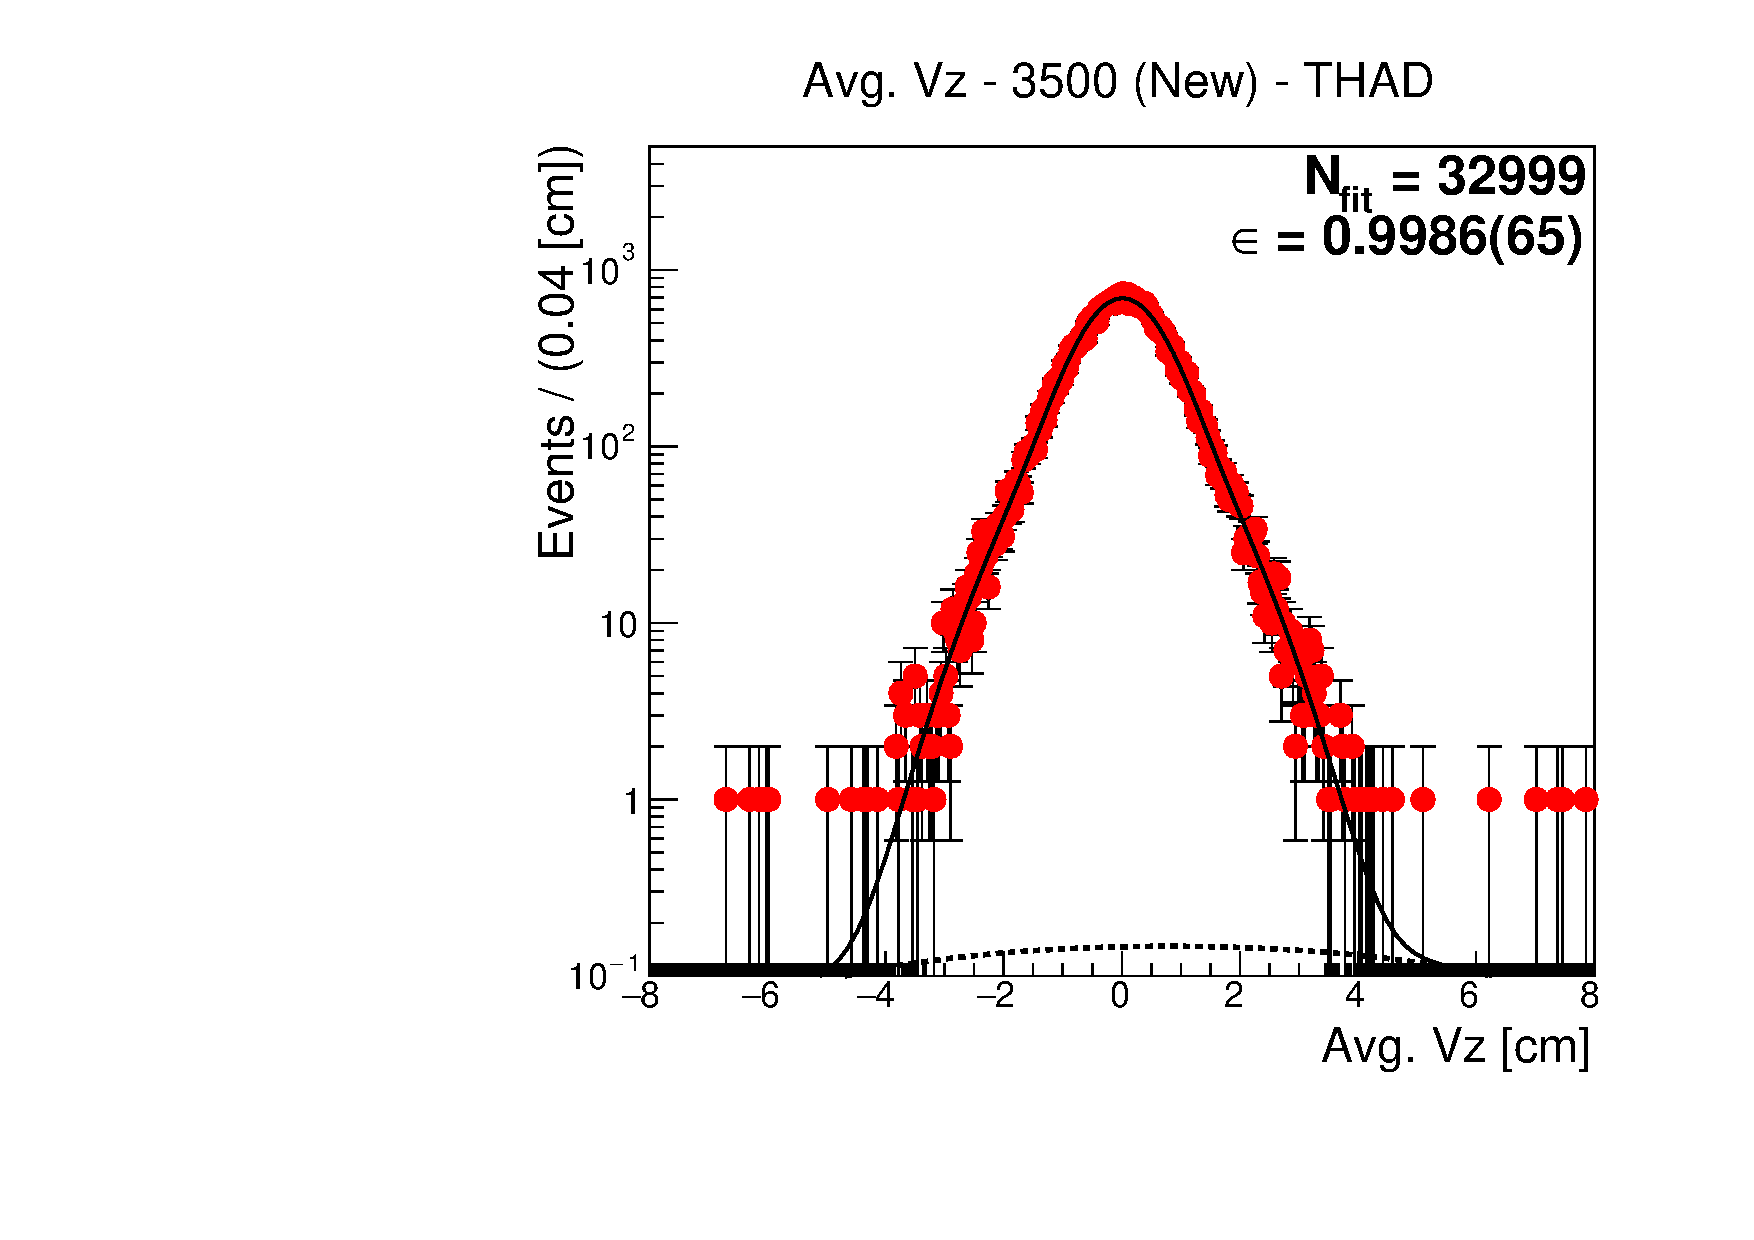
\includegraphics[scale=0.25]{figures/plots/nonDDbar_fit_results/3650_new/fit_new_3500_data_THAD.pdf}
\caption{The number of hadrons found in the 3500 (New) data sample.}
{This includes results for SHAD (left), LHAD (middle), and THAD (right).}
\label{fig:hadron_fits_3500_new}
\end{figure}


\begin{figure}[H]
\centering
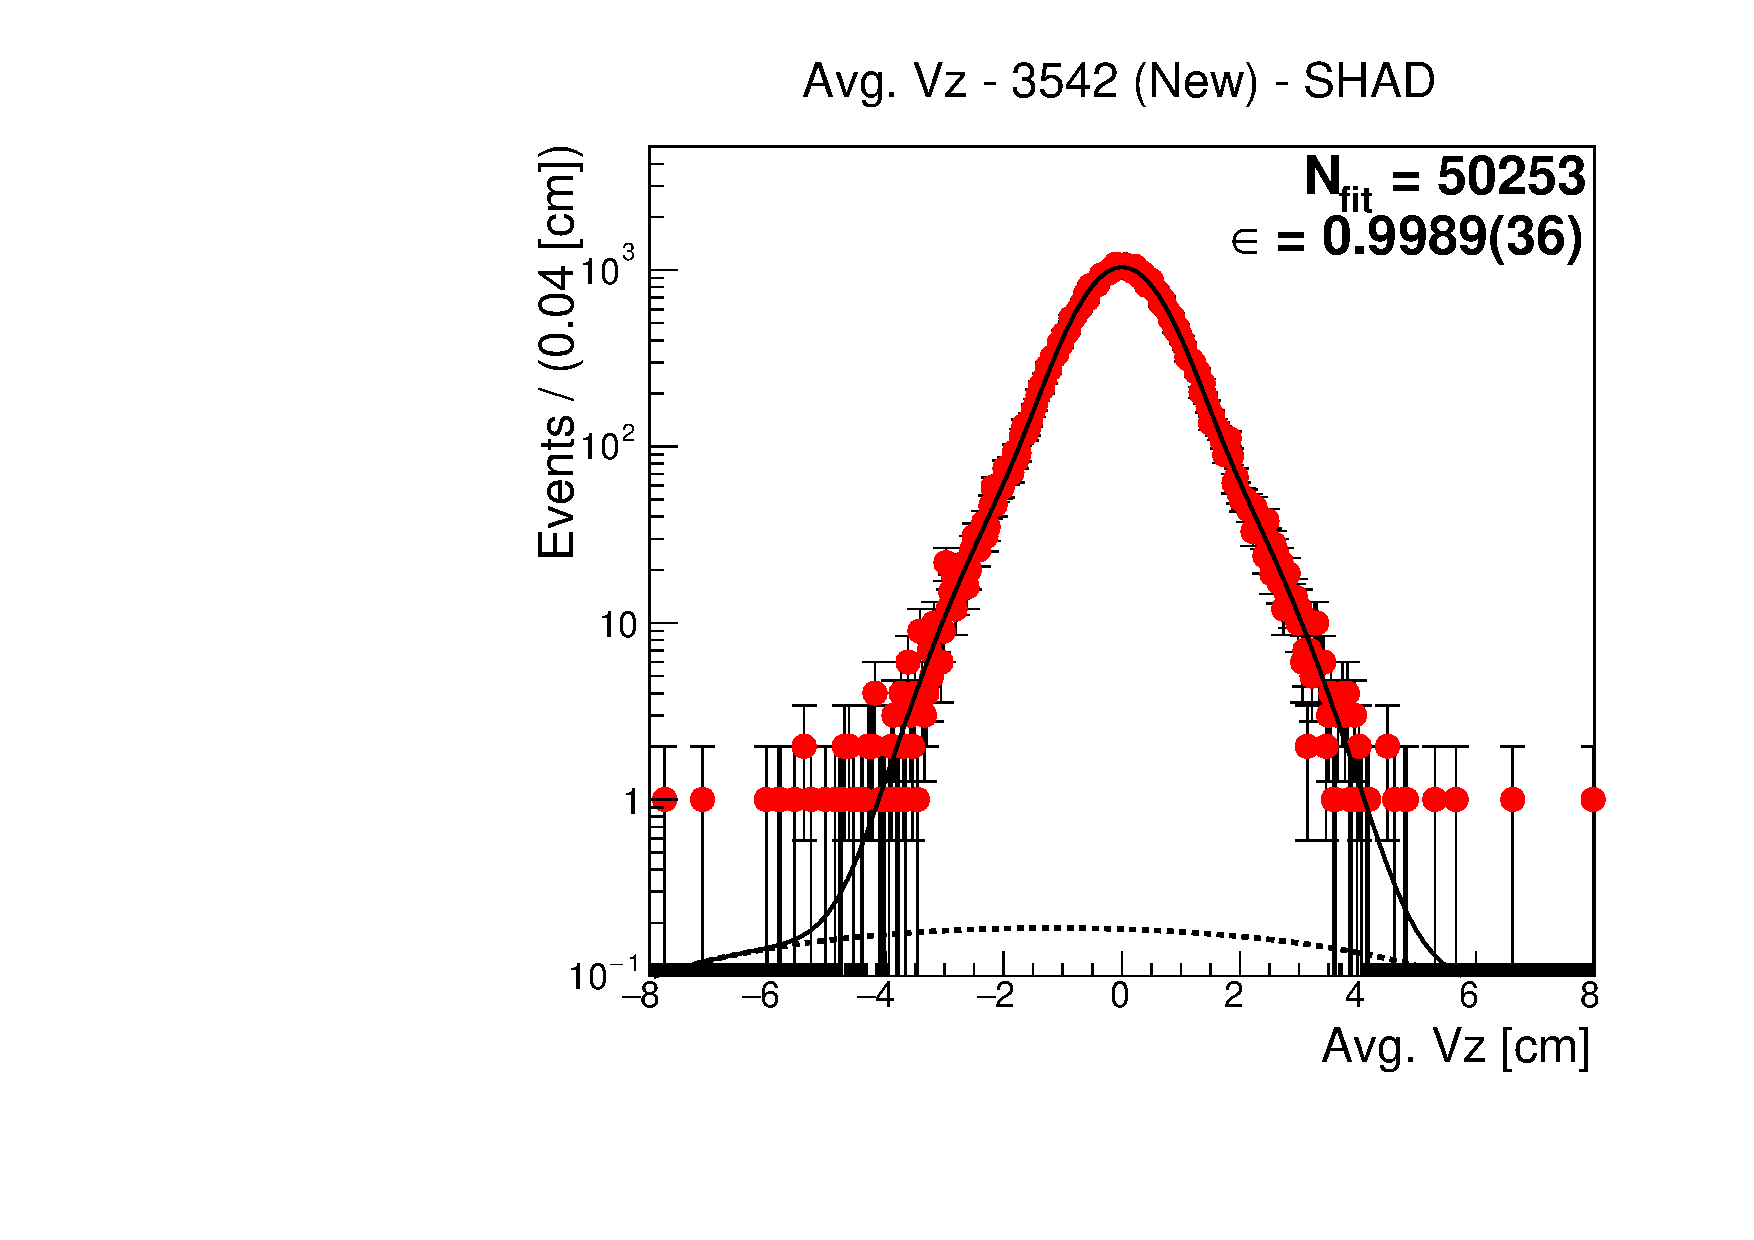
\includegraphics[scale=0.25]{figures/plots/nonDDbar_fit_results/3650_new/fit_new_3542_data_SHAD.pdf}
\hspace{-0.5cm}
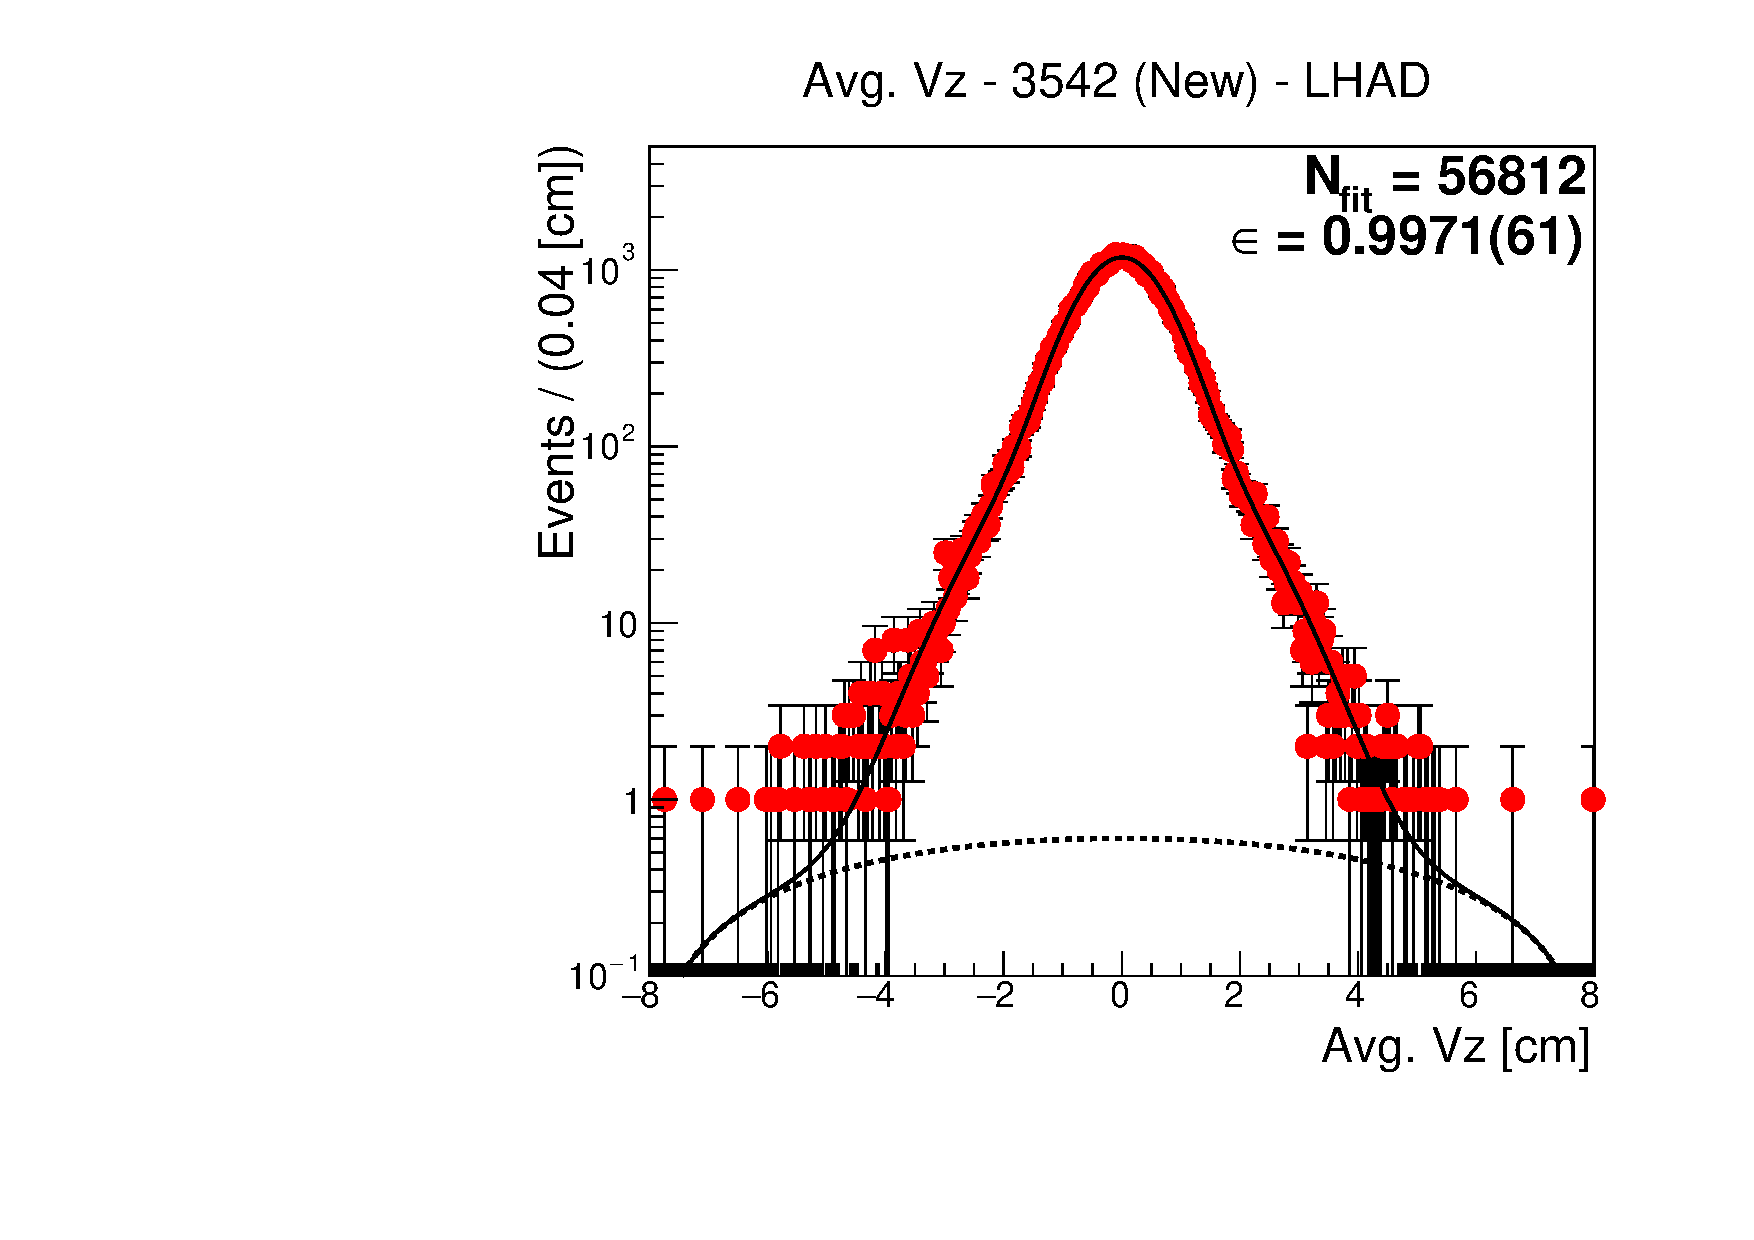
\includegraphics[scale=0.25]{figures/plots/nonDDbar_fit_results/3650_new/fit_new_3542_data_LHAD.pdf}
\hspace{-0.5cm}
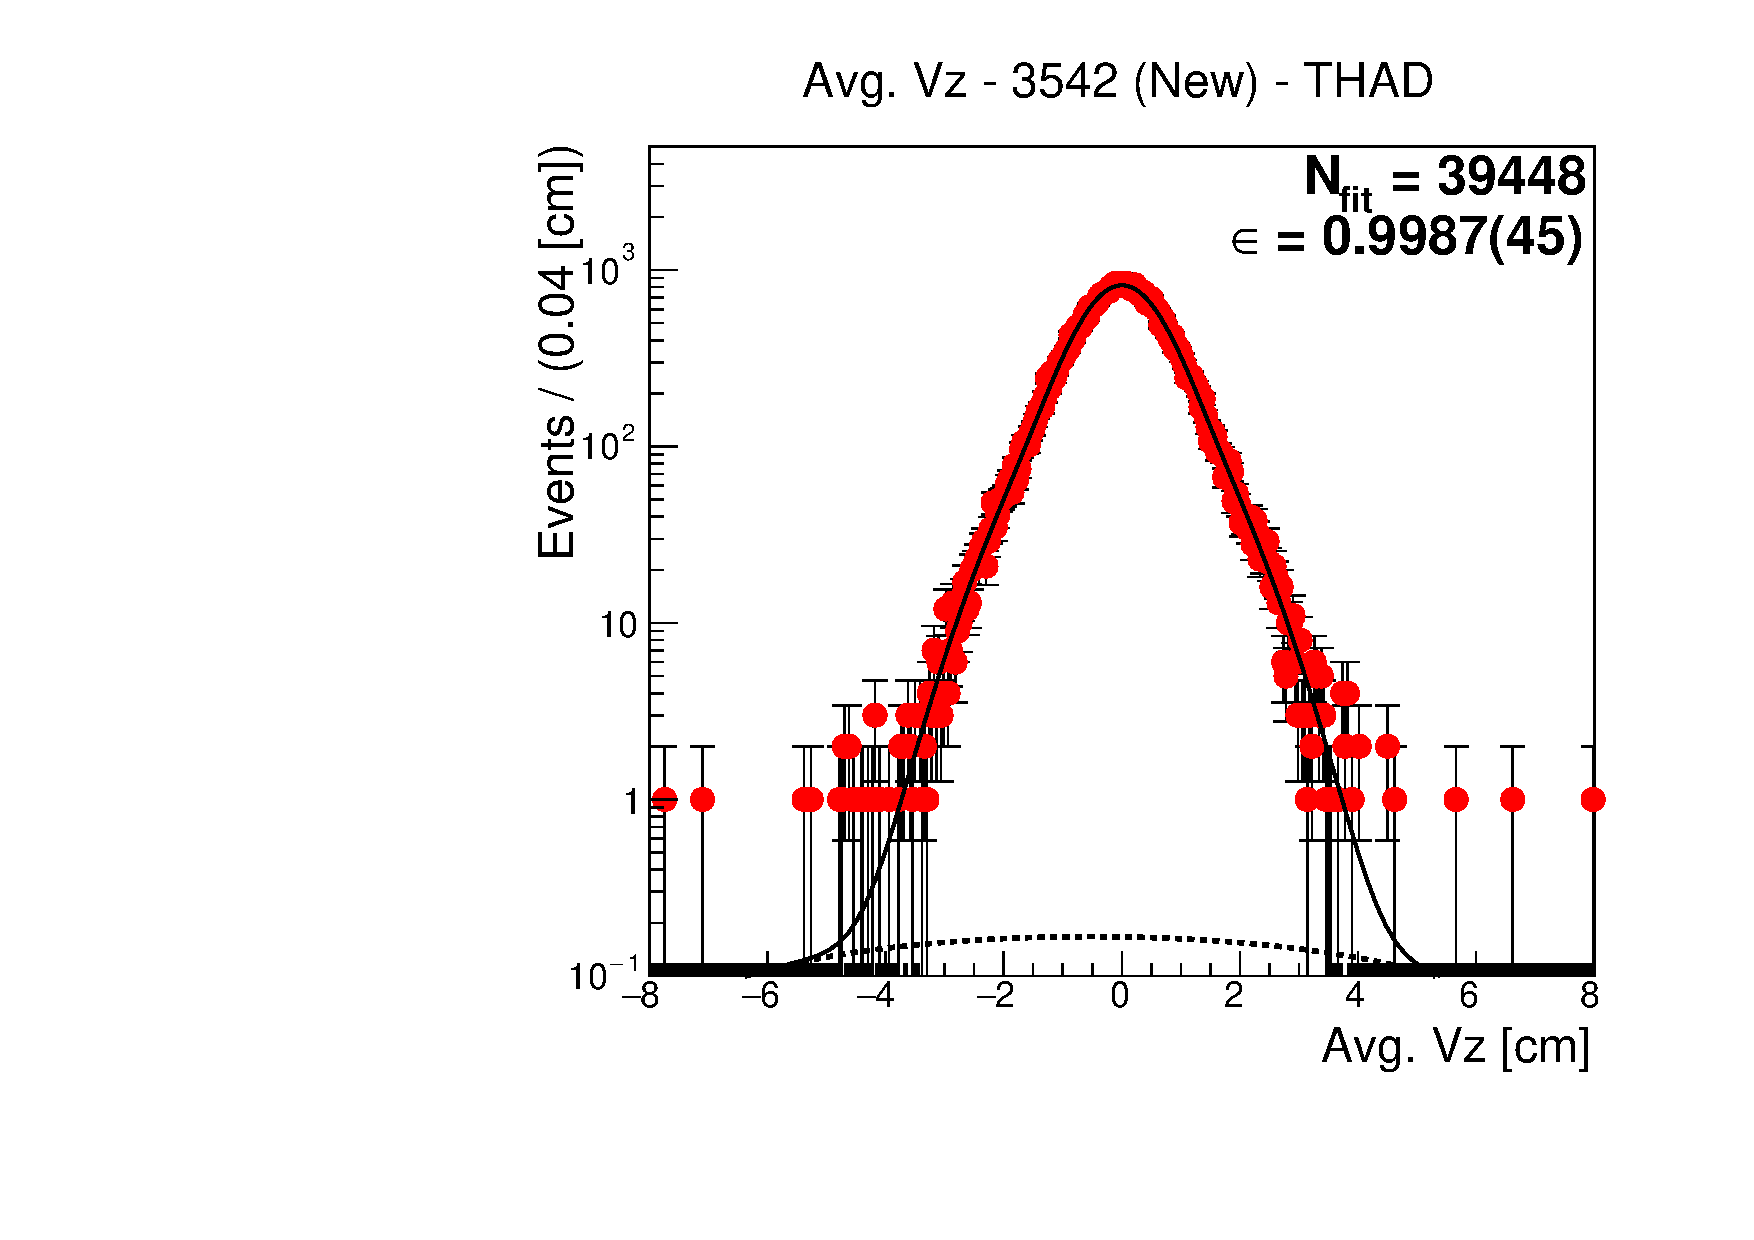
\includegraphics[scale=0.25]{figures/plots/nonDDbar_fit_results/3650_new/fit_new_3542_data_THAD.pdf}
\caption{The number of hadrons found in the 3542 (New) data sample.}
{This includes results for SHAD (left), LHAD (middle), and THAD (right).}
\label{fig:hadron_fits_3542_new}
\end{figure}


\begin{figure}[H]
\centering
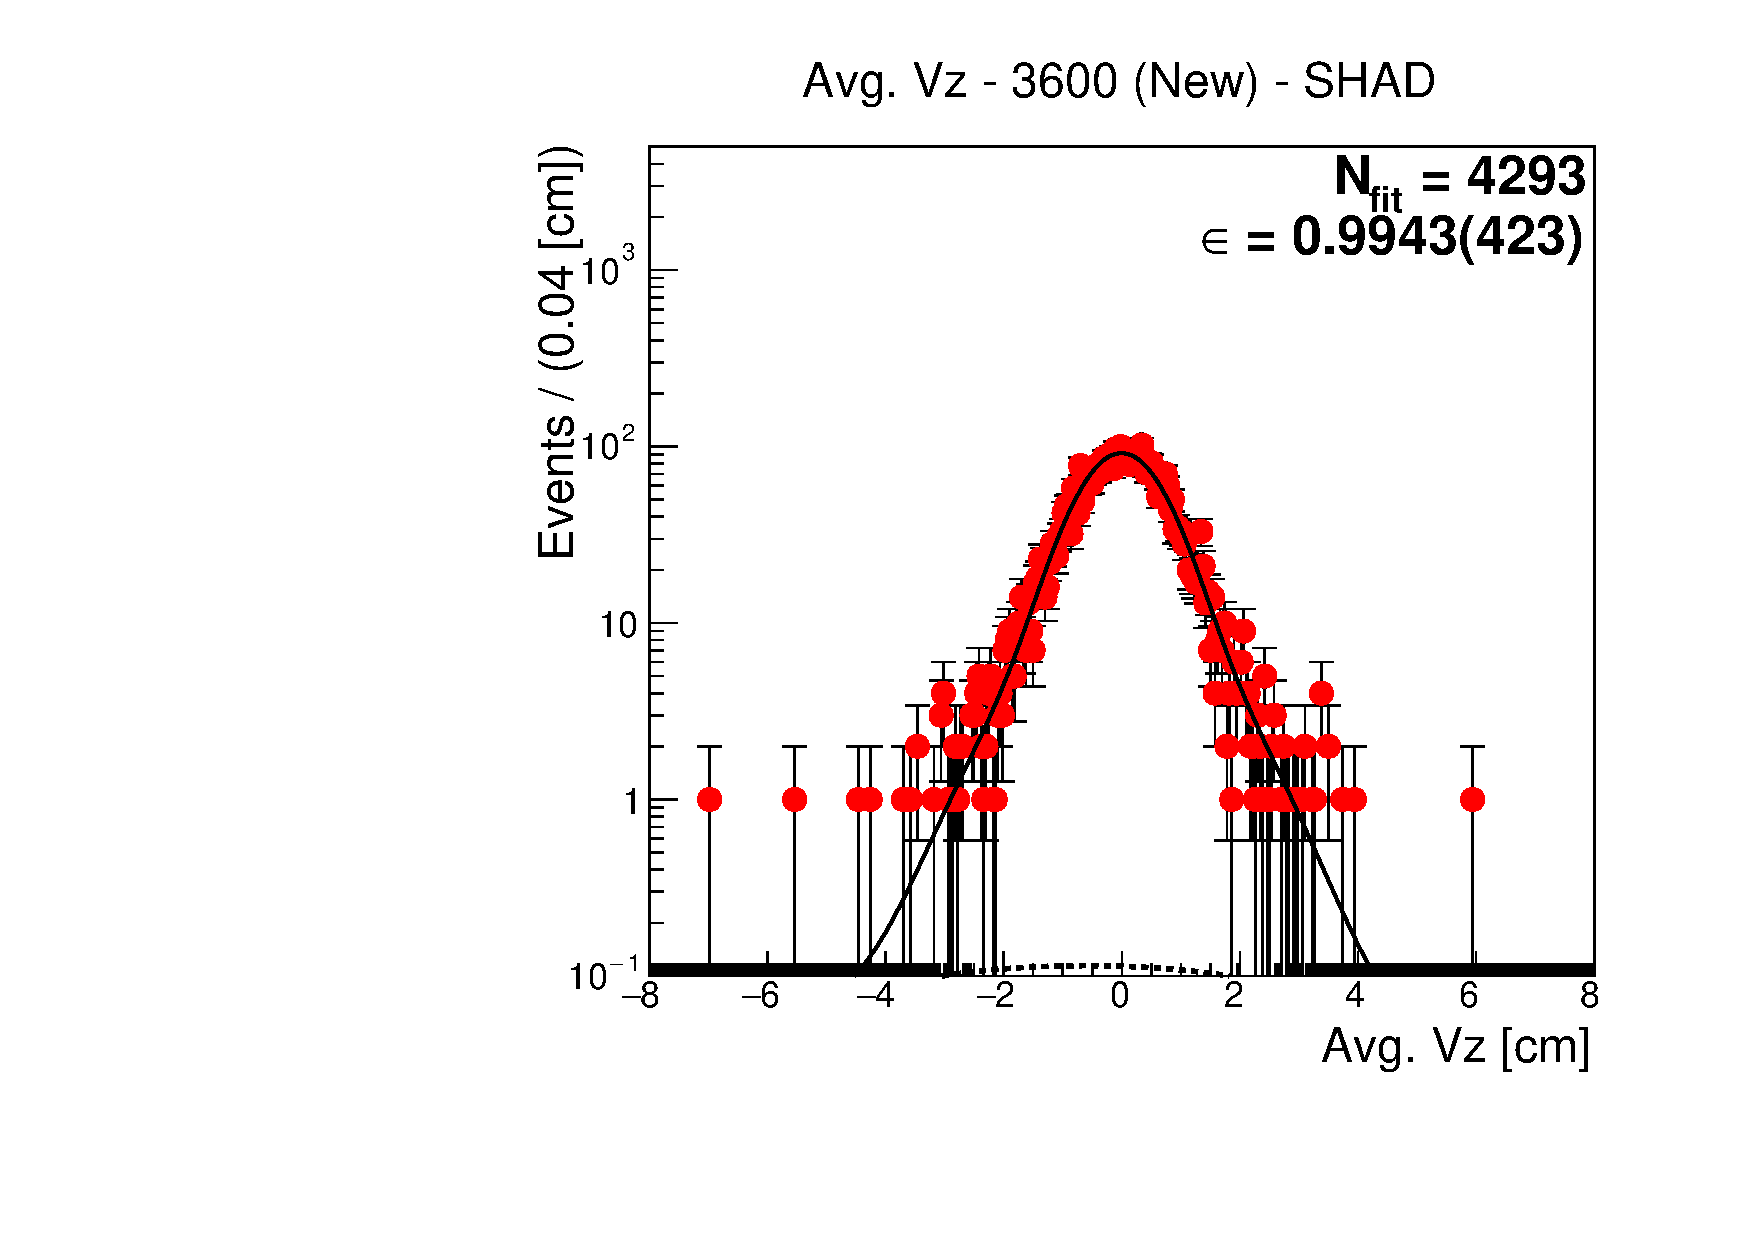
\includegraphics[scale=0.25]{figures/plots/nonDDbar_fit_results/3650_new/fit_new_3600_data_SHAD.pdf}
\hspace{-0.5cm}
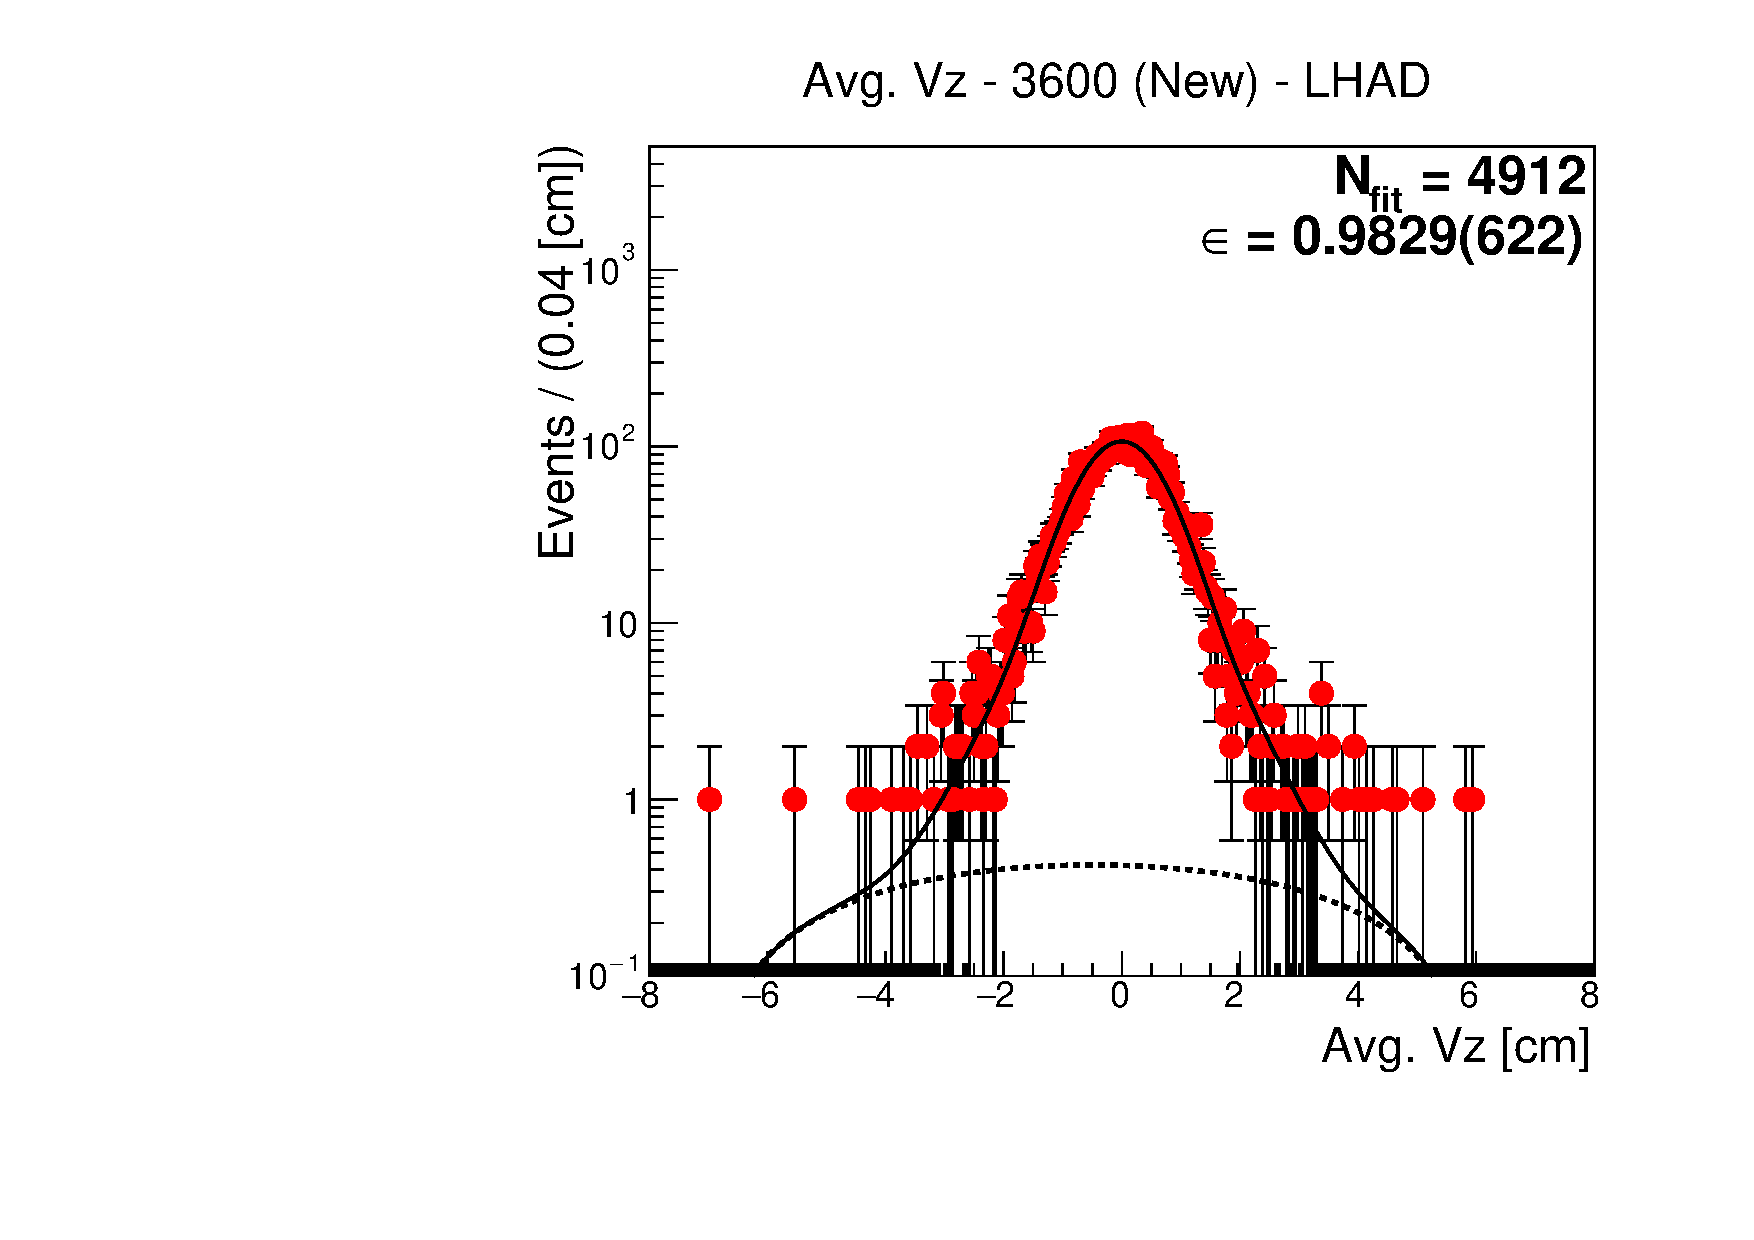
\includegraphics[scale=0.25]{figures/plots/nonDDbar_fit_results/3650_new/fit_new_3600_data_LHAD.pdf}
\hspace{-0.5cm}
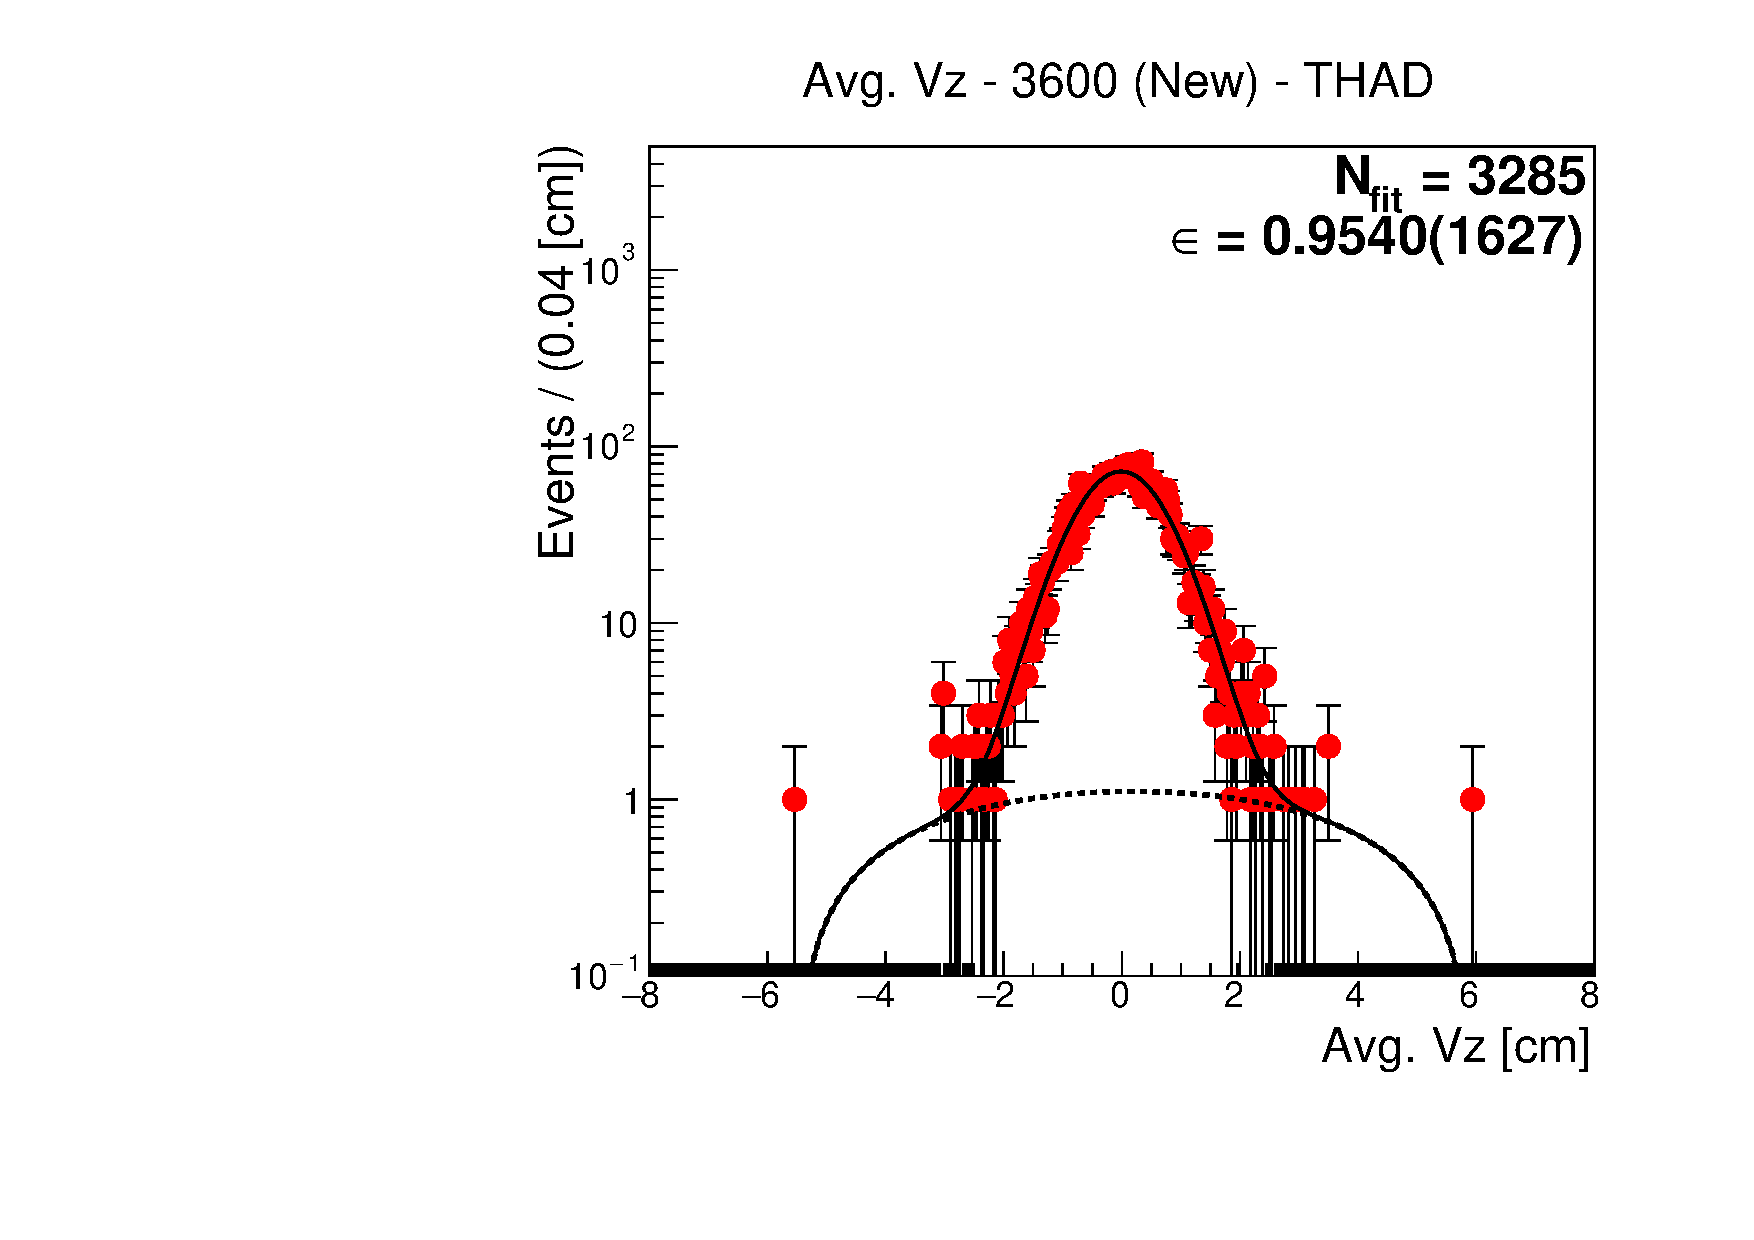
\includegraphics[scale=0.25]{figures/plots/nonDDbar_fit_results/3650_new/fit_new_3600_data_THAD.pdf}
\caption{The number of hadrons found in the 3600 (New) data sample.}
{This includes results for SHAD (left), LHAD (middle), and THAD (right).}
\label{fig:hadron_fits_3600_new}
\end{figure}


\begin{figure}[H]
\centering
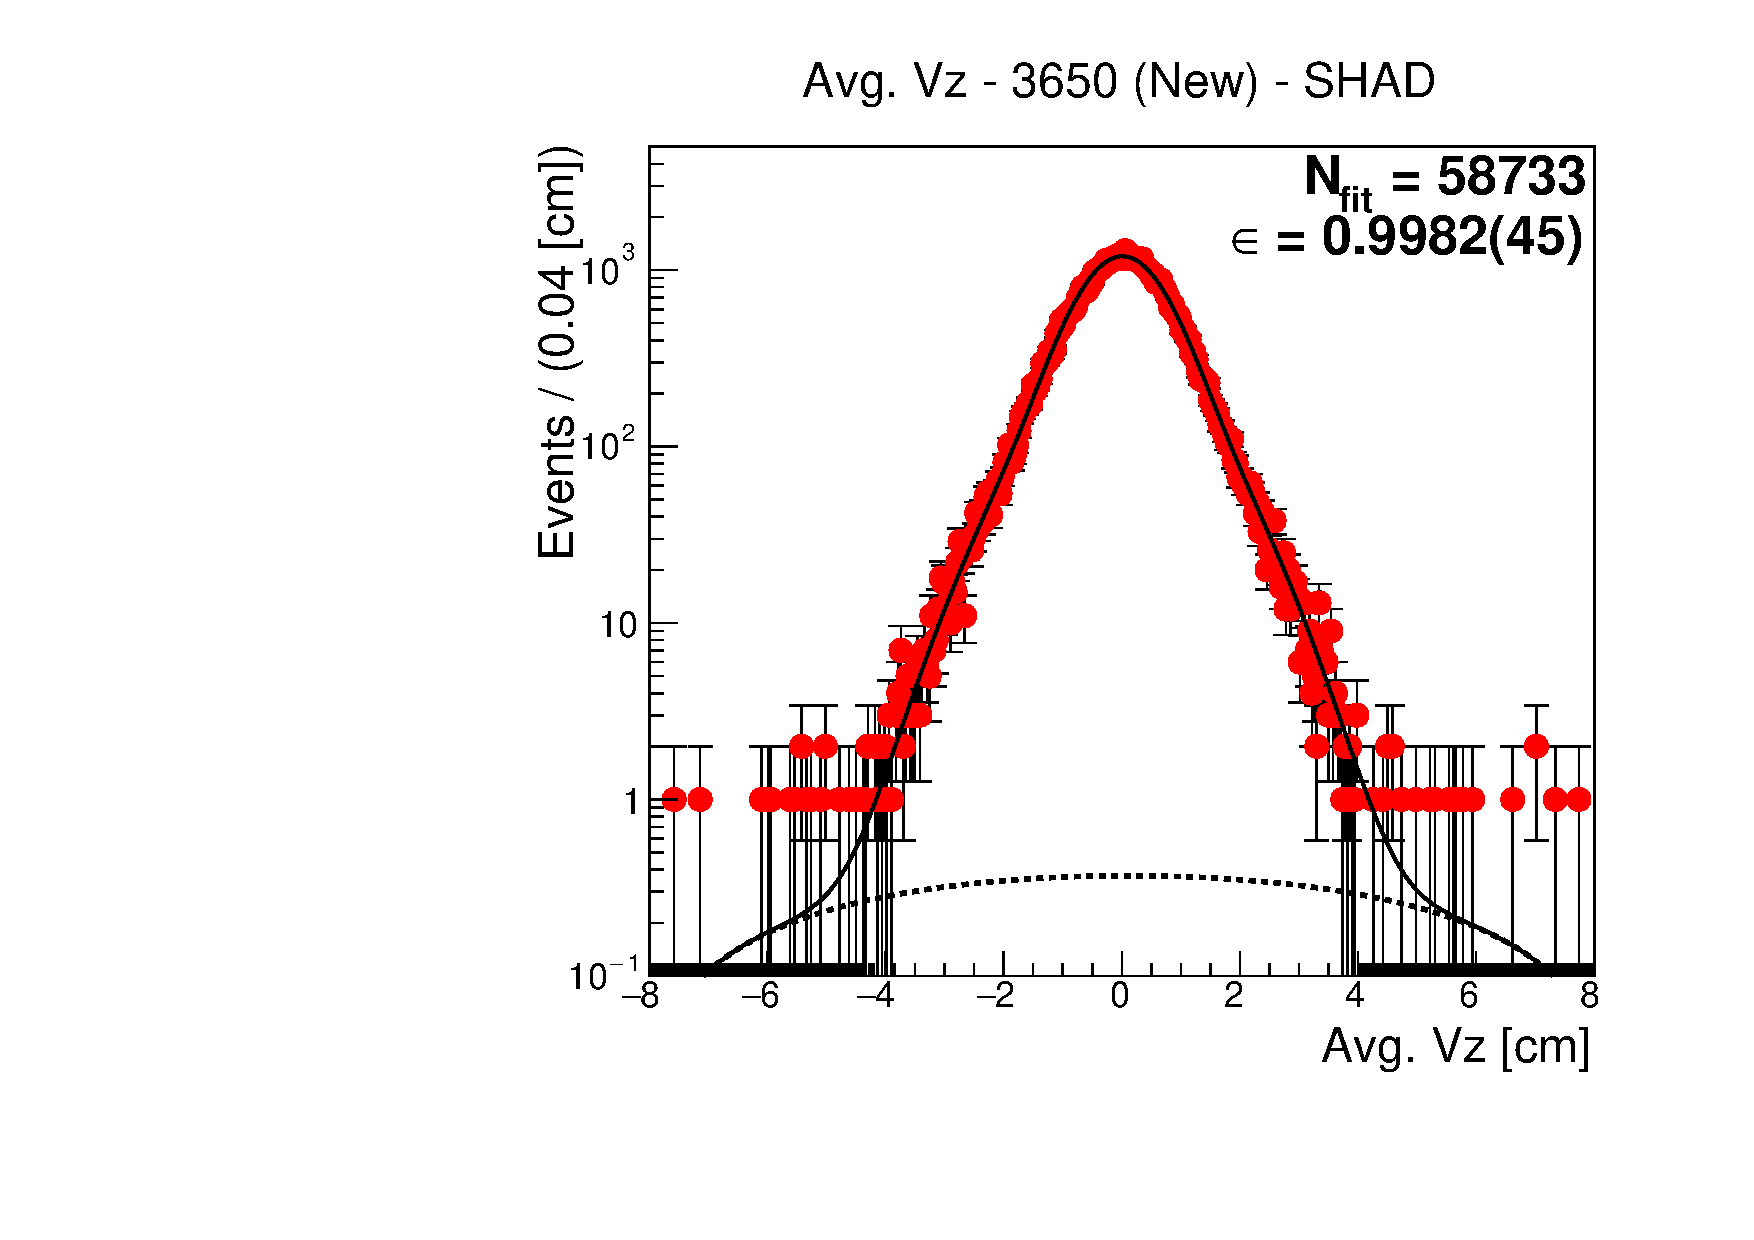
\includegraphics[scale=0.25]{figures/plots/nonDDbar_fit_results/3650_new/fit_new_3650_data_SHAD.pdf}
\hspace{-0.5cm}
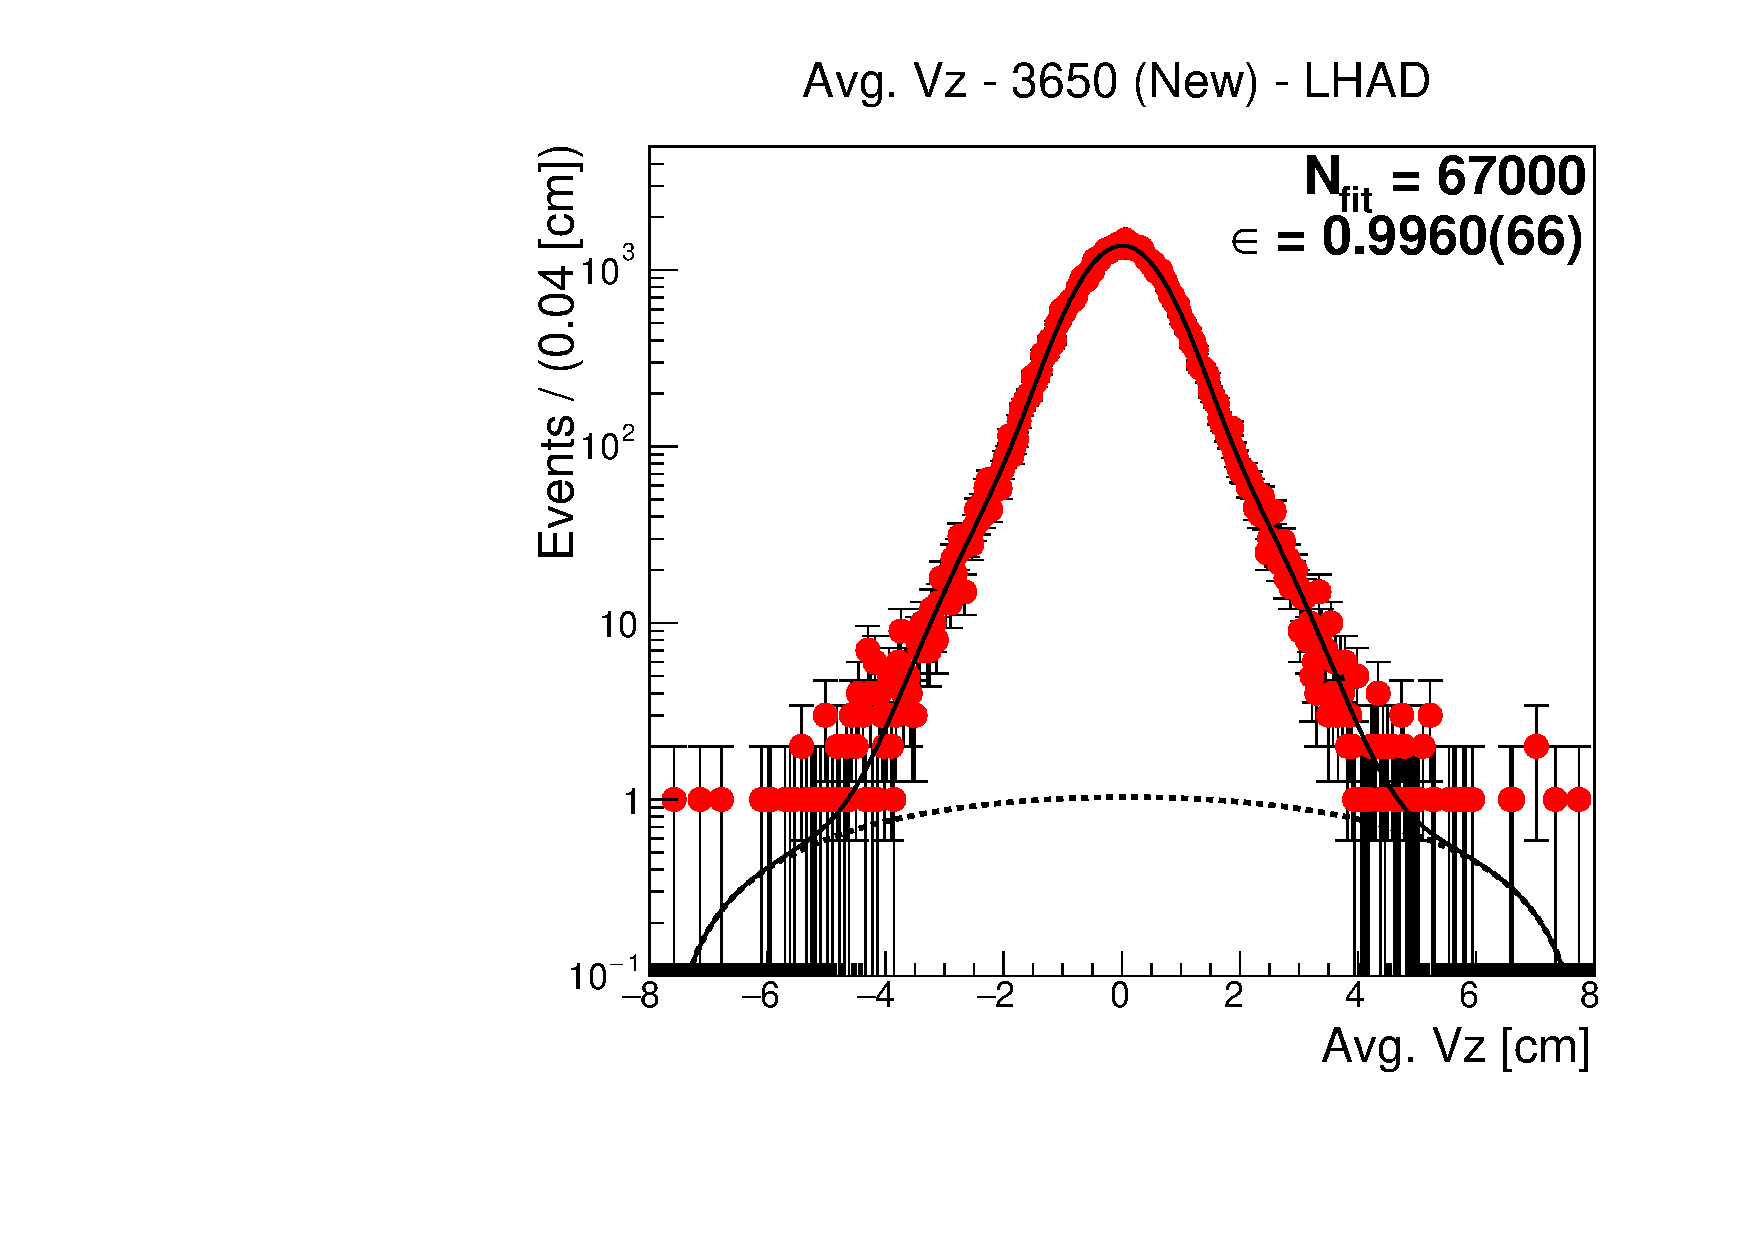
\includegraphics[scale=0.25]{figures/plots/nonDDbar_fit_results/3650_new/fit_new_3650_data_LHAD.pdf}
\hspace{-0.5cm}
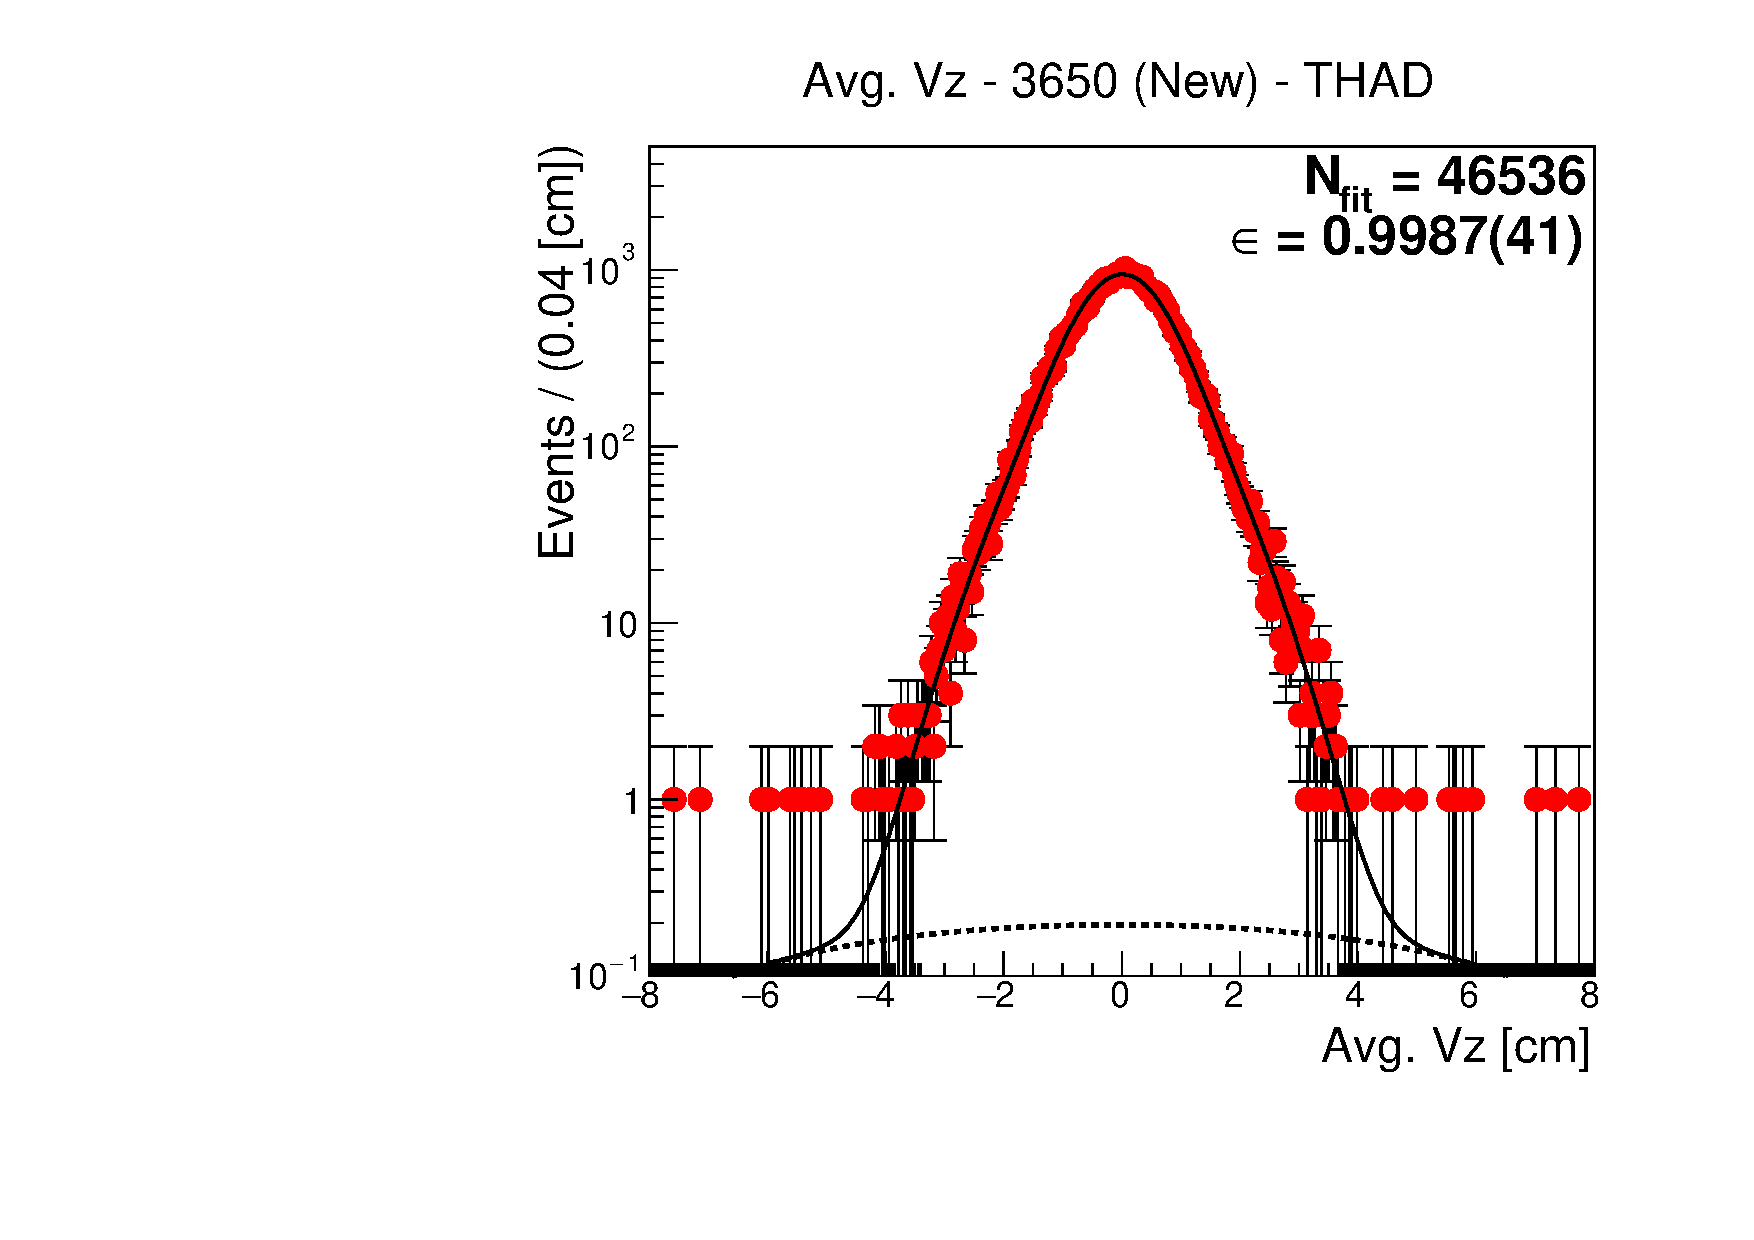
\includegraphics[scale=0.25]{figures/plots/nonDDbar_fit_results/3650_new/fit_new_3650_data_THAD.pdf}
\caption{The number of hadrons found in the 3650 (New) data sample.}
{This includes results for SHAD (left), LHAD (middle), and THAD (right).}
\label{fig:hadron_fits_3650_new}
\end{figure}


\begin{figure}[H]
\centering
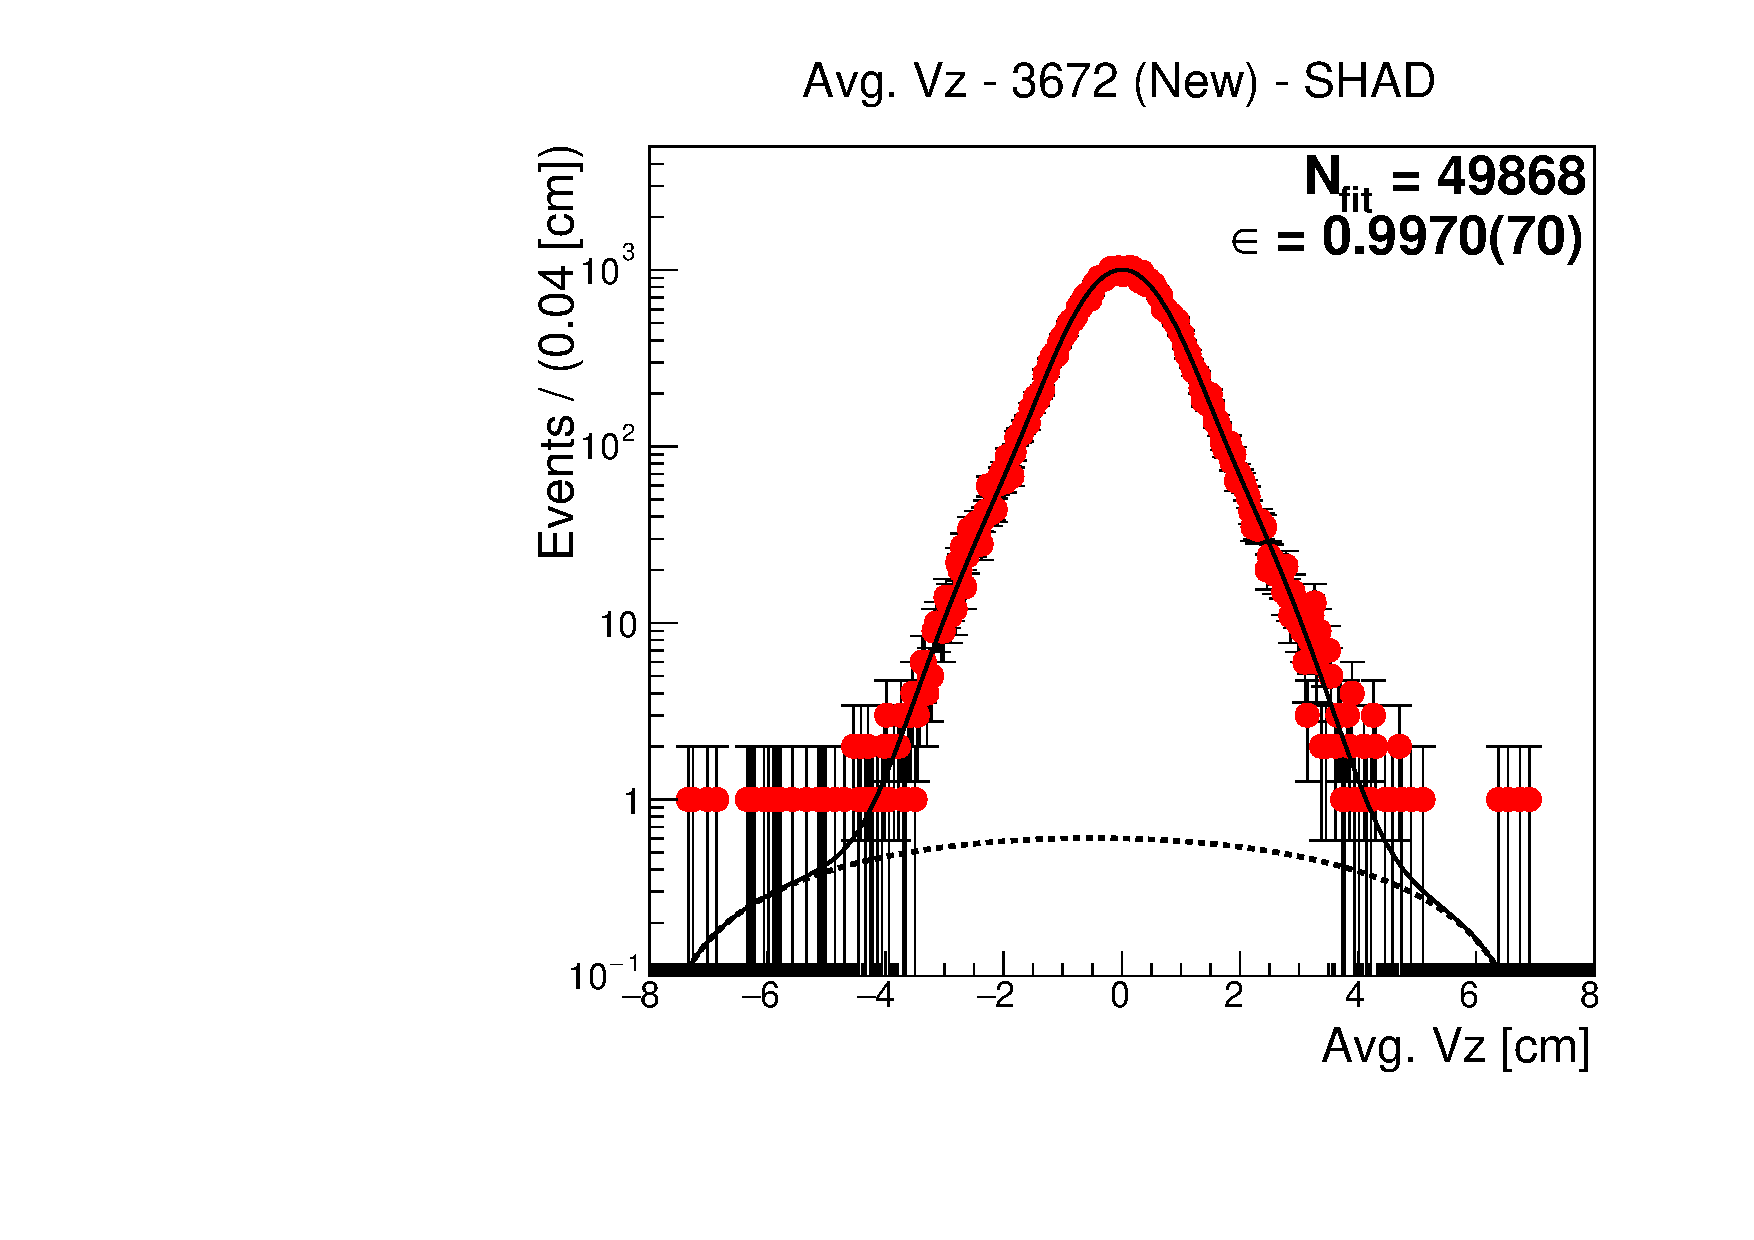
\includegraphics[scale=0.25]{figures/plots/nonDDbar_fit_results/3650_new/fit_new_3671_data_SHAD.pdf}
\hspace{-0.5cm}
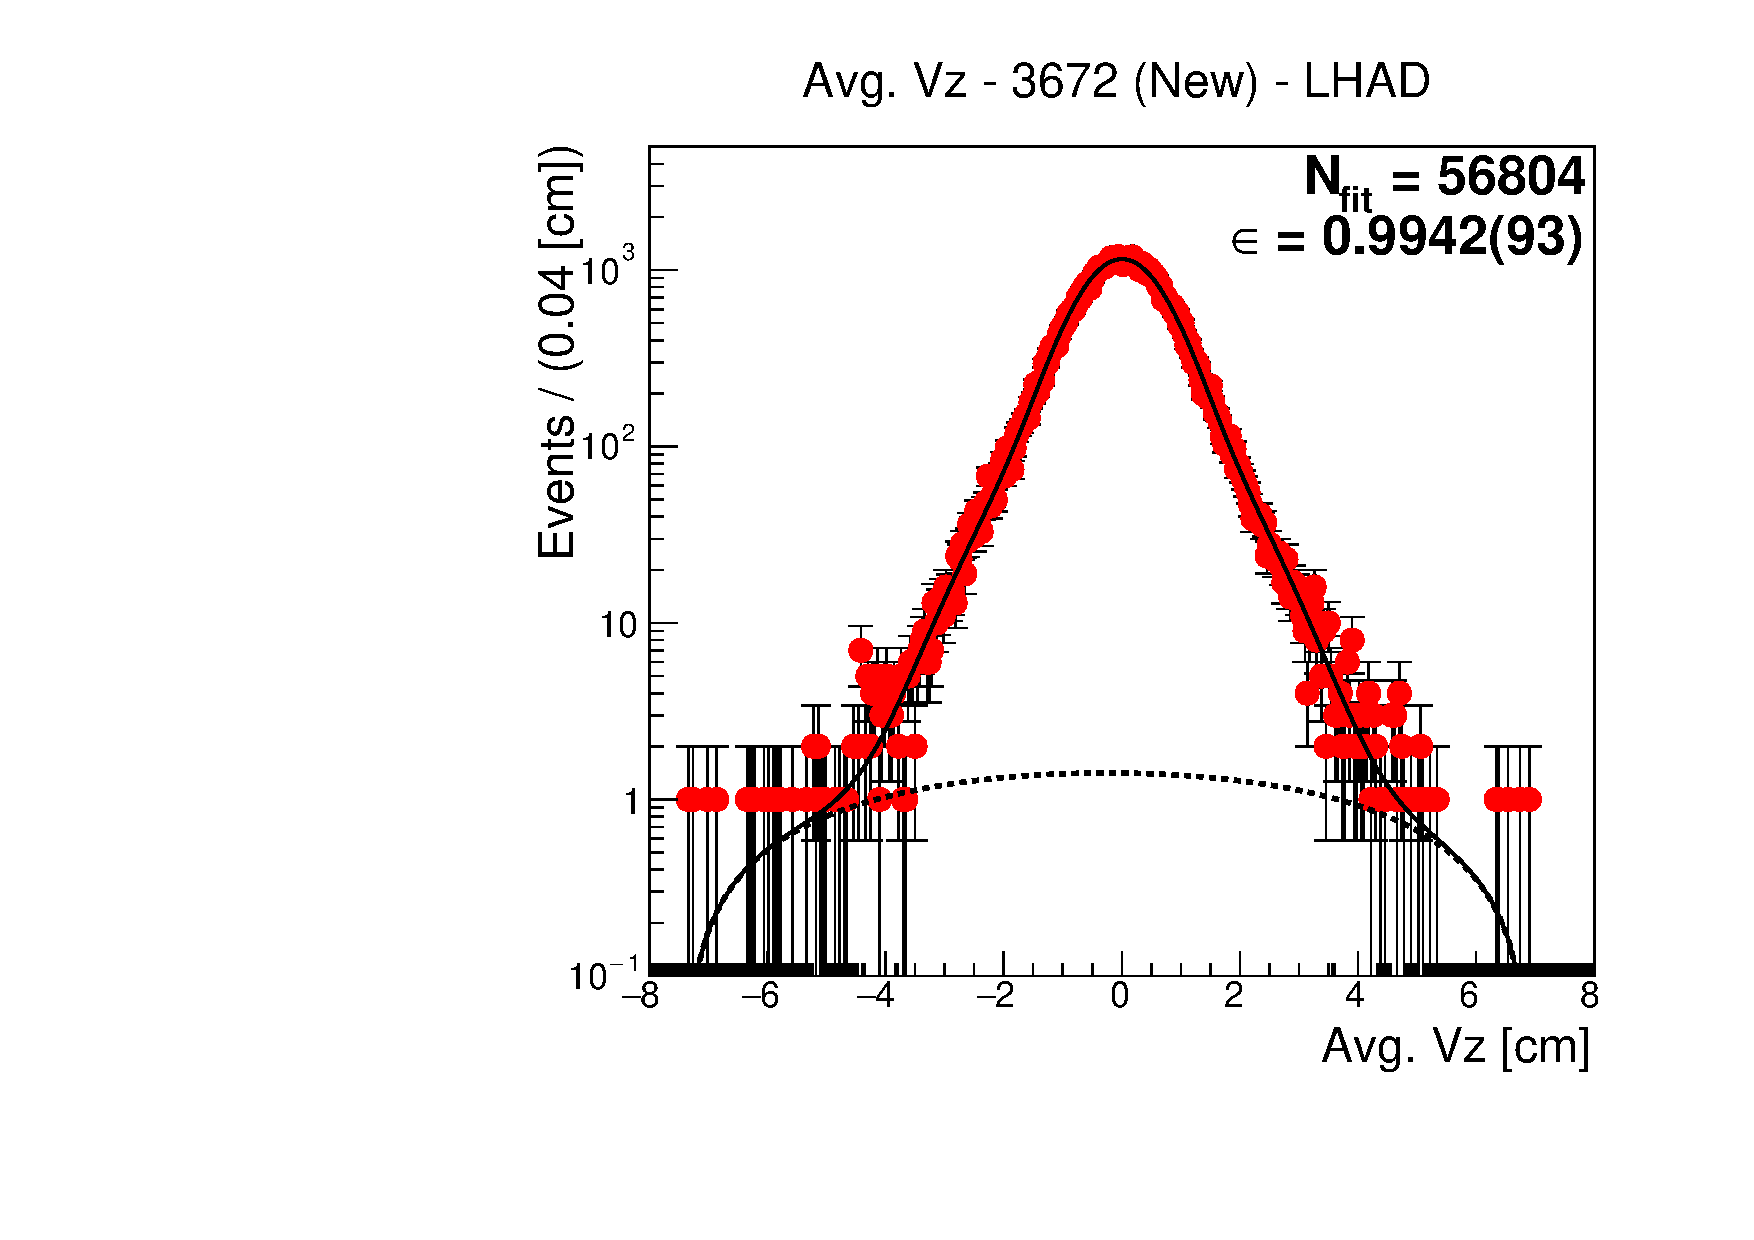
\includegraphics[scale=0.25]{figures/plots/nonDDbar_fit_results/3650_new/fit_new_3671_data_LHAD.pdf}
\hspace{-0.5cm}
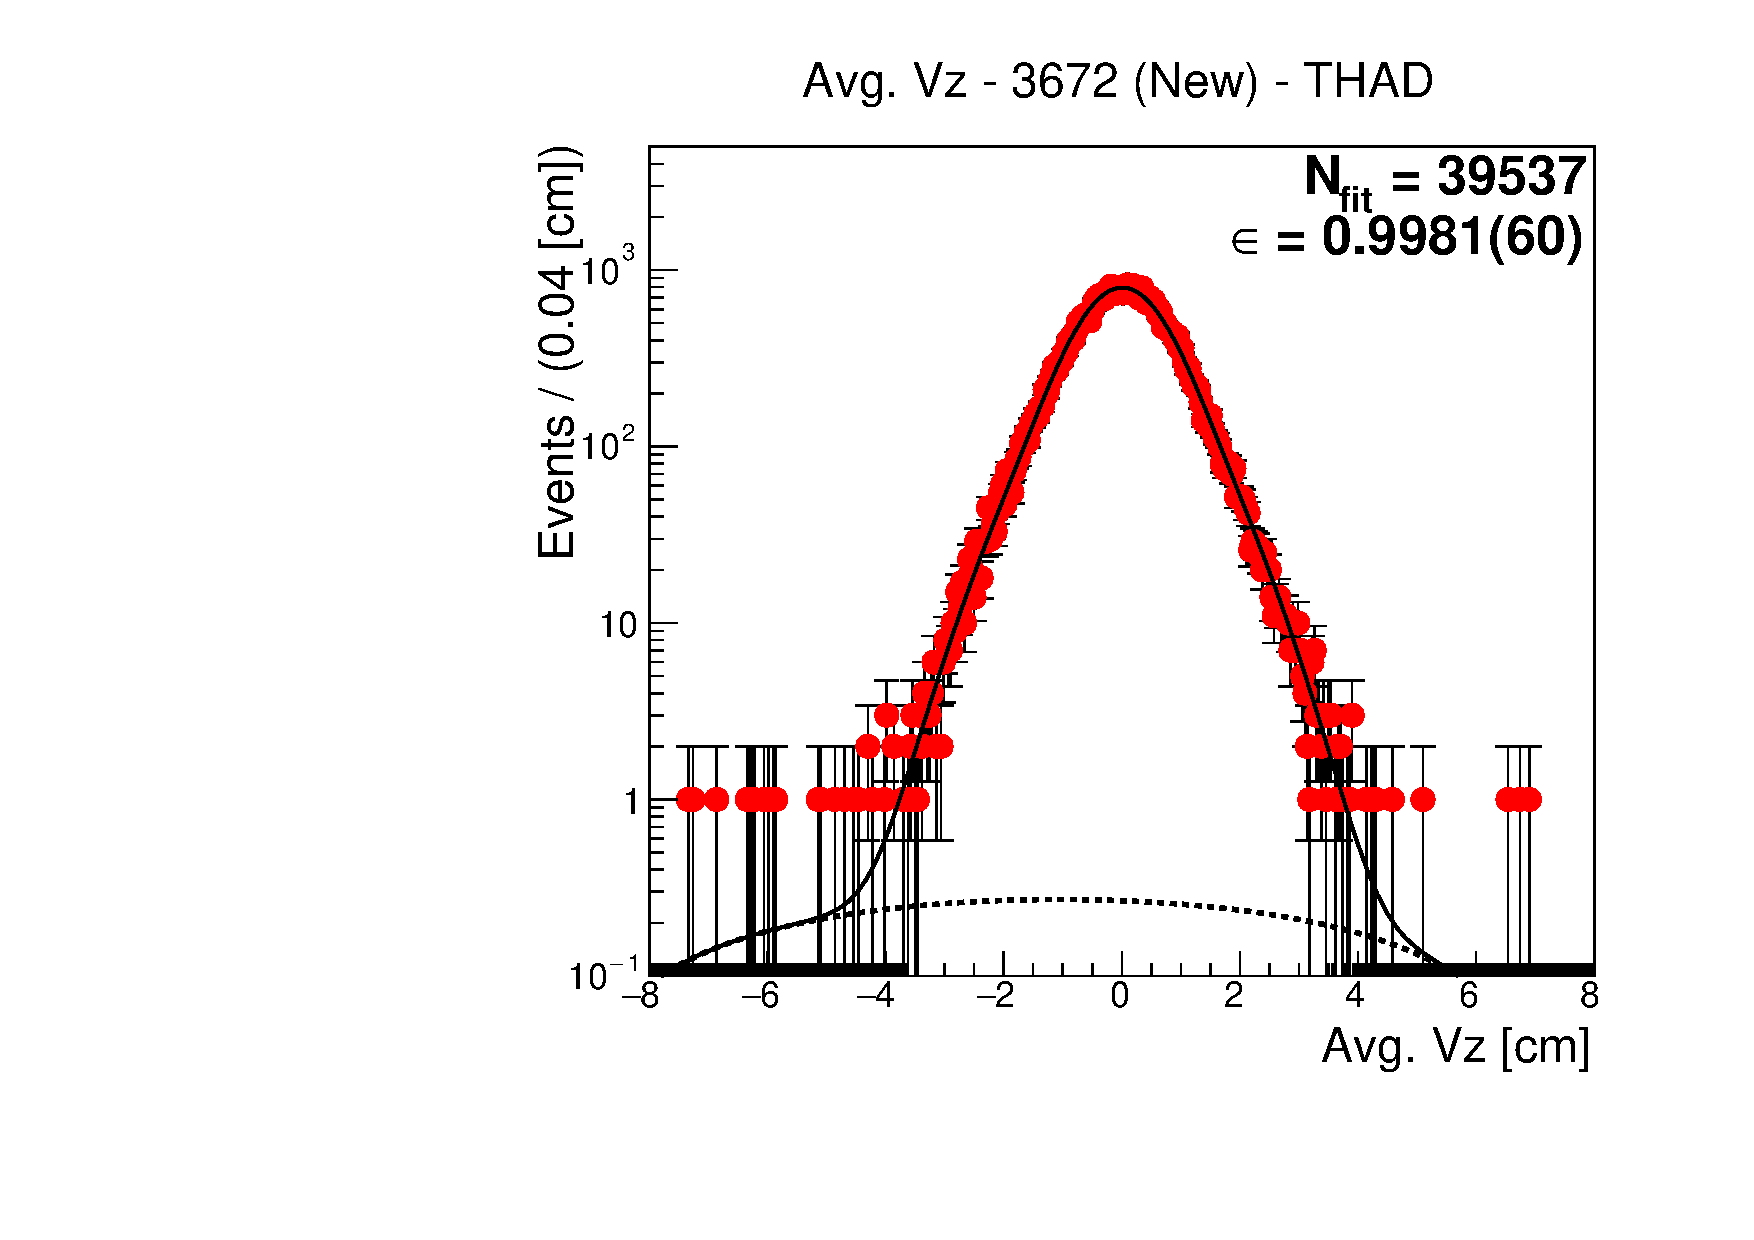
\includegraphics[scale=0.25]{figures/plots/nonDDbar_fit_results/3650_new/fit_new_3671_data_THAD.pdf}
\caption{The number of hadrons found in the 3671 (New) data sample.}
{This includes results for SHAD (left), LHAD (middle), and THAD (right).}
\label{fig:hadron_fits_3671_new}
\end{figure}



\begin{table}[H]
\centering
\renewcommand\arraystretch{1.0}

\begin{tabular}{c|r|cr@{$\; \pm \;$}rc cr@{$\; \pm \;$}rc cr@{$\; \pm \;$}rc}
\hline
\multicolumn{14}{c}{3500 (New) Reconstruction} \\
\hline
Sample & $\sigma$ [\si{\pb}] & \multicolumn{4}{c}{$\effmc$ (SHAD) [\%]} & \multicolumn{4}{c}{$\effmc$ (LHAD) [\%]} & \multicolumn{4}{c}{$\effmc$ (THAD) [\%]} \\
\hline
$\tautau$       & 0.000 && \mcd{2}         &&& \mcd{2}         &&& \mcd{2}         & \\
$\yjpsi$        & 1.831 &&  47.079 & 0.077 &&&  56.117 & 0.084 &&&  35.320 & 0.066 & \\
$\twophoton$    & 1.240 &&   2.380 & 0.017 &&&   4.924 & 0.025 &&&   1.644 & 0.014 & \\
$\psip^\dagger$ & 0.006 &&  62.989 & 0.008 &&&  69.288 & 0.008 &&&  51.694 & 0.007 & \\
\hline          
\end{tabular}

\vspace{0.5cm}

\begin{tabular}{c|r|cr@{$\; \pm \;$}rc cr@{$\; \pm \;$}rc cr@{$\; \pm \;$}rc}
\hline
\multicolumn{14}{c}{3542 (New) Reconstruction} \\
\hline
Sample & $\sigma$ [\si{\pb}] & \multicolumn{4}{c}{$\effmc$ (SHAD) [\%]} & \multicolumn{4}{c}{$\effmc$ (LHAD) [\%]} & \multicolumn{4}{c}{$\effmc$ (THAD) [\%]} \\
\hline
$\tautau$       & 0.000 && \mcd{2}        &&& \mcd{2}        &&& \mcd{2}        & \\
$\yjpsi$        & 1.632 && 47.188 & 0.072 &&& 56.430 & 0.079 &&& 35.355 & 0.063 & \\
$\twophoton$    & 1.270 &&  2.386 & 0.016 &&&  5.046 & 0.024 &&&  1.633 & 0.013 & \\
$\psip^\dagger$ & 0.009 && 62.989 & 0.008 &&& 69.288 & 0.008 &&& 51.694 & 0.007 & \\
\hline          
\end{tabular}

\vspace{0.5cm}

\begin{tabular}{c|r|cr@{$\; \pm \;$}rc cr@{$\; \pm \;$}rc cr@{$\; \pm \;$}rc}
\hline
\multicolumn{14}{c}{3600 (New) Reconstruction} \\
\hline
Sample & $\sigma$ [\si{\pb}] & \multicolumn{4}{c}{$\effmc$ (SHAD) [\%]} & \multicolumn{4}{c}{$\effmc$ (LHAD) [\%]} & \multicolumn{4}{c}{$\effmc$ (THAD) [\%]} \\
\hline
$\tautau$       & 1.262 && 12.851 & 0.080 &&& 29.096 & 0.121 &&& 10.040 & 0.071 & \\
$\yjpsi$        & 1.412 && 47.524 & 0.154 &&& 56.902 & 0.169 &&& 35.703 & 0.134 & \\
$\twophoton$    & 1.311 &&  2.651 & 0.036 &&&  5.089 & 0.050 &&&  1.897 & 0.031 & \\
$\psip^\dagger$ & 0.024 && 62.989 & 0.008 &&& 69.288 & 0.008 &&& 51.694 & 0.007 & \\
\hline          
\end{tabular}

\vspace{0.5cm}

\begin{tabular}{c|r|cr@{$\; \pm \;$}rc cr@{$\; \pm \;$}rc cr@{$\; \pm \;$}rc}
\hline
\multicolumn{14}{c}{3650 (New) Reconstruction} \\
\hline
Sample & $\sigma$ [\si{\pb}] & \multicolumn{4}{c}{$\effmc$ (SHAD) [\%]} & \multicolumn{4}{c}{$\effmc$ (LHAD) [\%]} & \multicolumn{4}{c}{$\effmc$ (THAD) [\%]} \\
\hline
$\tautau$       & 1.844 && 12.964 & 0.033 &&& 28.939 & 0.049 &&& 10.154 & 0.029 & \\
$\yjpsi$        & 1.260 && 47.414 & 0.063 &&& 57.043 & 0.069 &&& 35.701 & 0.055 & \\
$\twophoton$    & 1.346 &&  2.410 & 0.014 &&&  4.675 & 0.020 &&&  1.682 & 0.012 & \\
$\psip^\dagger$ & 0.110 && 62.989 & 0.008 &&& 69.288 & 0.008 &&& 51.694 & 0.007 & \\
\hline          
\end{tabular}

\vspace{0.5cm}

\begin{tabular}{c|r|cr@{$\; \pm \;$}rc cr@{$\; \pm \;$}rc cr@{$\; \pm \;$}rc}
\hline
\multicolumn{14}{c}{3671 (New) Reconstruction} \\
\hline
Sample & $\sigma$ [\si{\pb}] & \multicolumn{4}{c}{$\effmc$ (SHAD) [\%]} & \multicolumn{4}{c}{$\effmc$ (LHAD) [\%]} & \multicolumn{4}{c}{$\effmc$ (THAD) [\%]} \\
\hline
$\tautau$       & 2.026 && 12.997 & 0.047 &&& 28.851 & 0.069 &&& 10.169 & 0.041 & \\
$\yjpsi$        & 1.205 && 47.496 & 0.089 &&& 57.237 & 0.098 &&& 35.745 & 0.077 & \\
$\twophoton$    & 1.361 &&  2.473 & 0.020 &&&  4.787 & 0.028 &&&  1.698 & 0.017 & \\
$\psip^\dagger$ & 0.436 && 62.989 & 0.008 &&& 69.288 & 0.008 &&& 51.694 & 0.007 & \\
\hline          
\end{tabular}

\caption{Reconstruction of background samples for the new continuum data.}
{$^\dagger$ The $\psip$ is assumed to have a standard Breit-Wigner shape.}
\label{tab:3650_new_reconstruction}
\end{table}

\begin{table}[H]
\centering
\renewcommand\arraystretch{1.0}

\begin{tabular}{c|cr@{$\; \pm \;$}rc cr@{$\; \pm \;$}rc cr@{$\; \pm \;$}rc}
\hline
\multicolumn{13}{c}{3500 (New) Results} \\
\hline
Sample         & \multicolumn{4}{c}{$\Nhad$ (SHAD)} & \multicolumn{4}{c}{$\Nhad$ (LHAD)} & \multicolumn{4}{c}{$\Nhad$ (THAD)} \\
\hline
Data            && 42106 & 205 &&& 47942 & 219 &&& 32999 & 182 & \\
$\yjpsi$        &&  3173 &  10 &&&  3782 &  11 &&&  2380 &   8 & \\
$\twophoton$    &&   109 &   1 &&&   225 &   1 &&&    75 &   1 & \\
$\psip^\dagger$ &&     5 &   1 &&&     5 &   1 &&&     4 &   1 & \\
\hline                                                         
Total           && 38820 & 205 &&& 43930 & 219 &&& 30540 & 182 & \\
\hline
\end{tabular}

\vspace{0.5cm}

\begin{tabular}{c|cr@{$\; \pm \;$}rc cr@{$\; \pm \;$}rc cr@{$\; \pm \;$}rc}
\hline
\multicolumn{13}{c}{3542 (New) Results} \\
\hline
Sample         & \multicolumn{4}{c}{$\Nhad$ (SHAD)} & \multicolumn{4}{c}{$\Nhad$ (LHAD)} & \multicolumn{4}{c}{$\Nhad$ (THAD)} \\
\hline
Data            && 50253 & 224 &&& 56812 & 238 &&& 39448 & 199 & \\
$\yjpsi$        &&  3450 &   9 &&&  4126 &  10 &&&  2585 &   7 & \\
$\twophoton$    &&   136 &   1 &&&   287 &   1 &&&    93 &   1 & \\
$\psip^\dagger$ &&    10 &   1 &&&    11 &   1 &&&     8 &   1 & \\
\hline                                                         
Total           && 46657 & 224 &&& 52388 & 239 &&& 36762 & 199 & \\
\hline
\end{tabular}

\vspace{0.5cm}

\begin{tabular}{c|cr@{$\; \pm \;$}rc cr@{$\; \pm \;$}rc cr@{$\; \pm \;$}rc}
\hline
\multicolumn{13}{c}{3600 (New) Results} \\
\hline
Sample         & \multicolumn{4}{c}{$\Nhad$ (SHAD)} & \multicolumn{4}{c}{$\Nhad$ (LHAD)} & \multicolumn{4}{c}{$\Nhad$ (THAD)} \\
\hline
Data            && 4293 & 66 &&& 4912 & 70 &&& 3285 & 57 & \\
$\tautau$       &&   64 &  3 &&&  145 &  7 &&&   50 &  2 & \\
$\yjpsi$        &&  265 & 13 &&&  317 & 16 &&&  199 & 10 & \\
$\twophoton$    &&   14 &  1 &&&   26 &  1 &&&   10 &  1 & \\
$\psip^\dagger$ &&    2 &  1 &&&    3 &  1 &&&    2 &  1 & \\
\hline                                               
Total           && 3948 & 67 &&& 4421 & 72 &&& 3024 & 58 & \\
\hline
\end{tabular}

\vspace{0.5cm}

\begin{tabular}{c|cr@{$\; \pm \;$}rc cr@{$\; \pm \;$}rc cr@{$\; \pm \;$}rc}
\hline
\multicolumn{13}{c}{3650 (New) Results} \\
\hline
Sample         & \multicolumn{4}{c}{$\Nhad$ (SHAD)} & \multicolumn{4}{c}{$\Nhad$ (LHAD)} & \multicolumn{4}{c}{$\Nhad$ (THAD)} \\
\hline
Data            && 58733 & 242 &&& 67000 & 259 &&& 46536 & 216 & \\
$\tautau$       &&  1295 &   4 &&&  2892 &   7 &&&  1015 &   3 & \\
$\yjpsi$        &&  3239 &   7 &&&  3896 &   8 &&&  2439 &   6 & \\
$\twophoton$    &&   176 &   1 &&&   341 &   2 &&&   123 &   1 & \\
$\psip^\dagger$ &&   148 &   1 &&&   163 &   1 &&&   121 &   1 & \\
\hline                                                         
Total           && 53875 & 242 &&& 59709 & 259 &&& 42839 & 216 & \\
\hline
\end{tabular}

\vspace{0.5cm}

\begin{tabular}{c|cr@{$\; \pm \;$}rc cr@{$\; \pm \;$}rc cr@{$\; \pm \;$}rc}
\hline
\multicolumn{13}{c}{3671 (New) Results} \\
\hline
Sample         & \multicolumn{4}{c}{$\Nhad$ (SHAD)} & \multicolumn{4}{c}{$\Nhad$ (LHAD)} & \multicolumn{4}{c}{$\Nhad$ (THAD)} \\
\hline
Data            && 49868 & 223 &&& 56804 & 238 &&& 39537 & 199 & \\
$\tautau$       &&  1229 &   5 &&&  2729 &   8 &&&   962 &   4 & \\
$\yjpsi$        &&  2671 &   7 &&&  3219 &   8 &&&  2010 &   6 & \\
$\twophoton$    &&   157 &   1 &&&   304 &   2 &&&   108 &   1 & \\
$\psip^\dagger$ &&   509 &   3 &&&   560 &   3 &&&   418 &   2 & \\
\hline                                                         
Total           && 45301 & 224 &&& 49991 & 239 &&& 36039 & 199 & \\
\hline
\end{tabular}

\caption{Hadronic events selected in the new continuum data.}
{$^\dagger$ The $\psip$ is assumed to have a standard Breit-Wigner shape.}
\label{tab:3650_new_results}
\end{table}


The reconstruction efficiency for a given $\Ecm$ point (in \si{\MeV}) can be calculated relative to the 3650 (Old) sample as follows:
\beq
\frac{ \epsilon(\Ecm) }{ \epsilon(3650) } = \left[ \frac{ \Nhad(\Ecm) }{ \Nhad(3650) } \right] \left[ \frac{ \lum(3650) }{ \lum(\Ecm) } \right] \bigg[ \frac{ \Ecm }{ 3650 } \bigg]^2.
\eeq
This value is calculated for each of the new continuum points, and a linear fit is performed for each of the selection cut methods.
From this slope, we can extrapolate to find the expected number of hadronic events for the scan data.
As the old continuum data was taken at a relatively similar time as the scan data, we use it as a normalization point for the efficiency extrapolation.
The results for each cut are shown in \Cref{fig:extrapolation_SHAD,fig:extrapolation_LHAD,fig:extrapolation_THAD}, where the dashed black line is the fit to the new continuum, and the solid green line is the extrapolation to higher energies.

\begin{figure}[H]
\centering
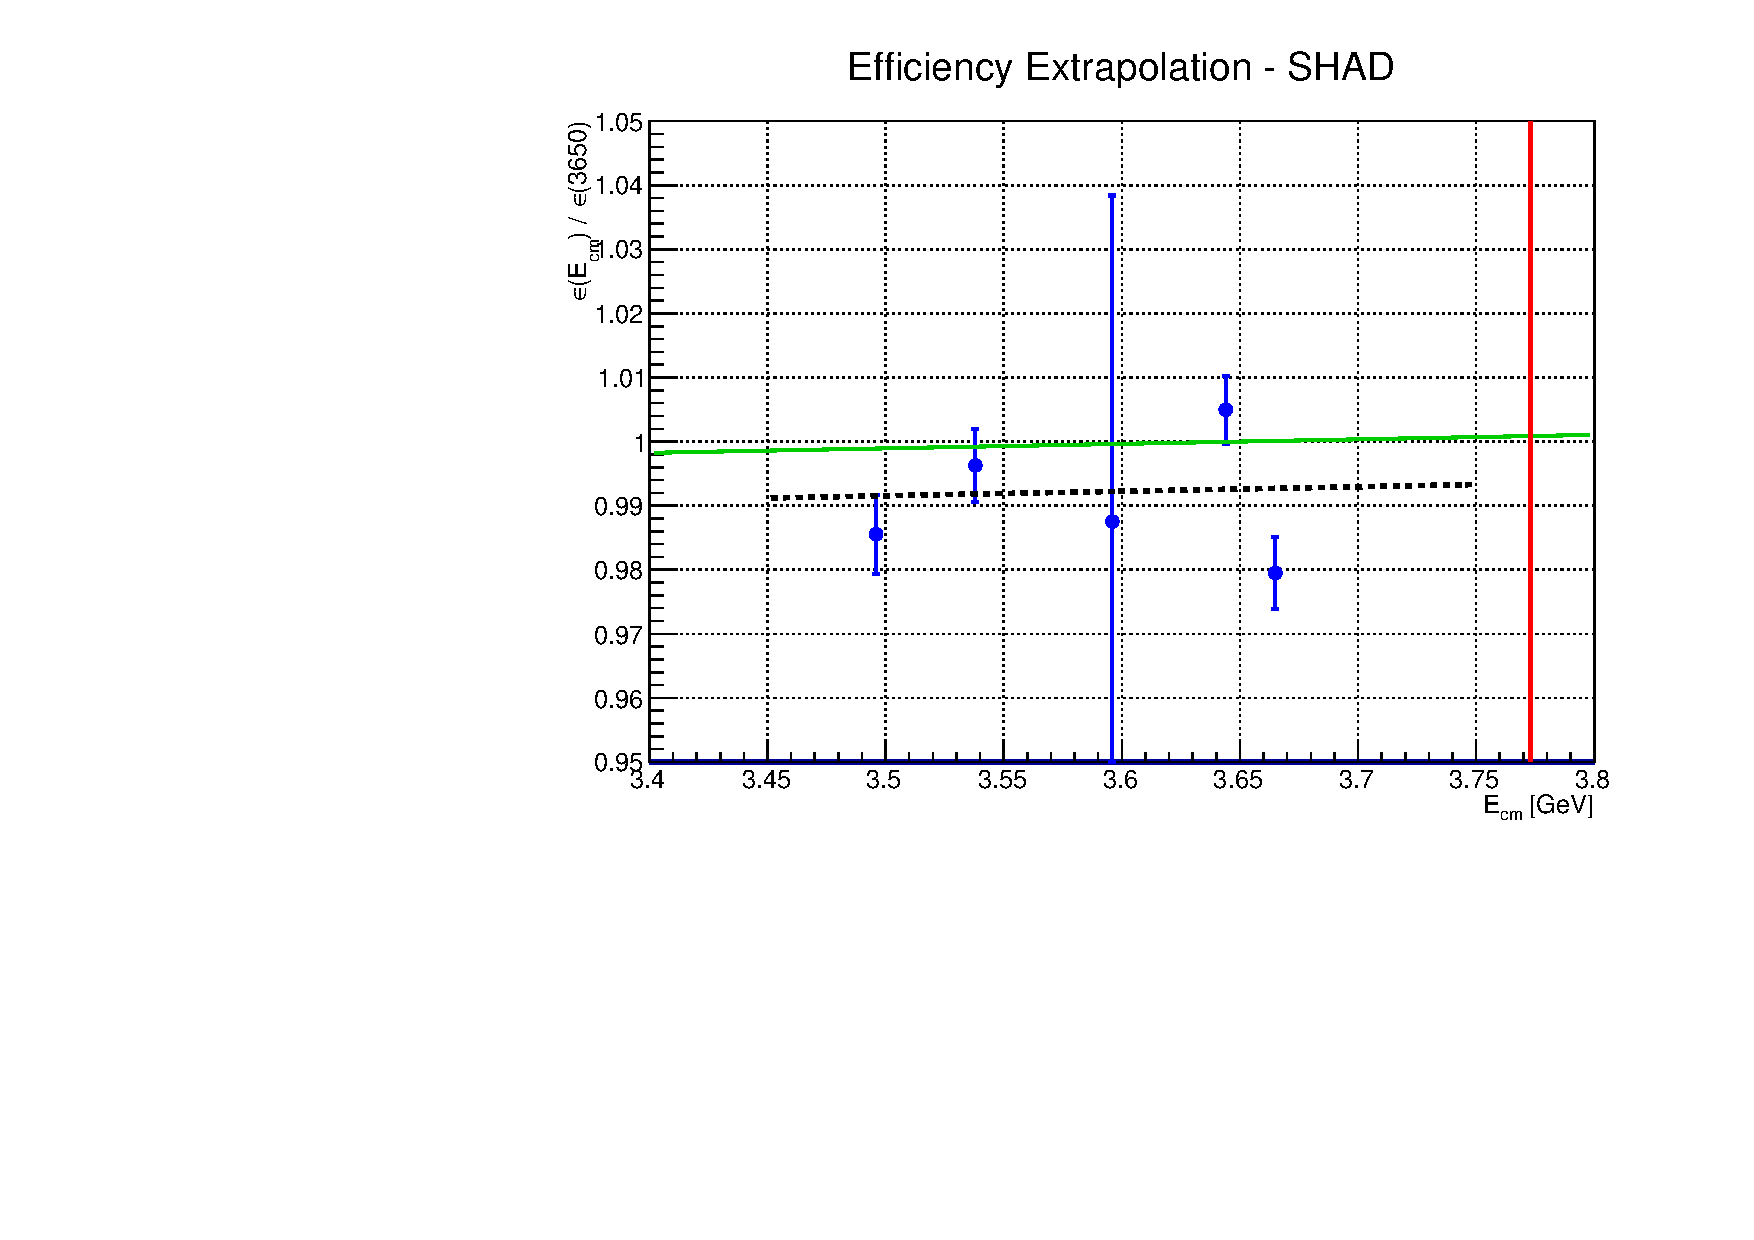
\includegraphics[scale=0.75]{figures/plots/SHAD_psip_BW.pdf}
\caption{The extrapolation for SHAD events using the new continuum data.}
{The new continuum points are fit to a linear slope (dashed black), then extrapolated to higher energies from the old continuum point (solid green). The energy of the $\psipp$ samples (solid red) is also shown.}
\label{fig:extrapolation_SHAD}
\end{figure}

\begin{figure}[H]
\centering
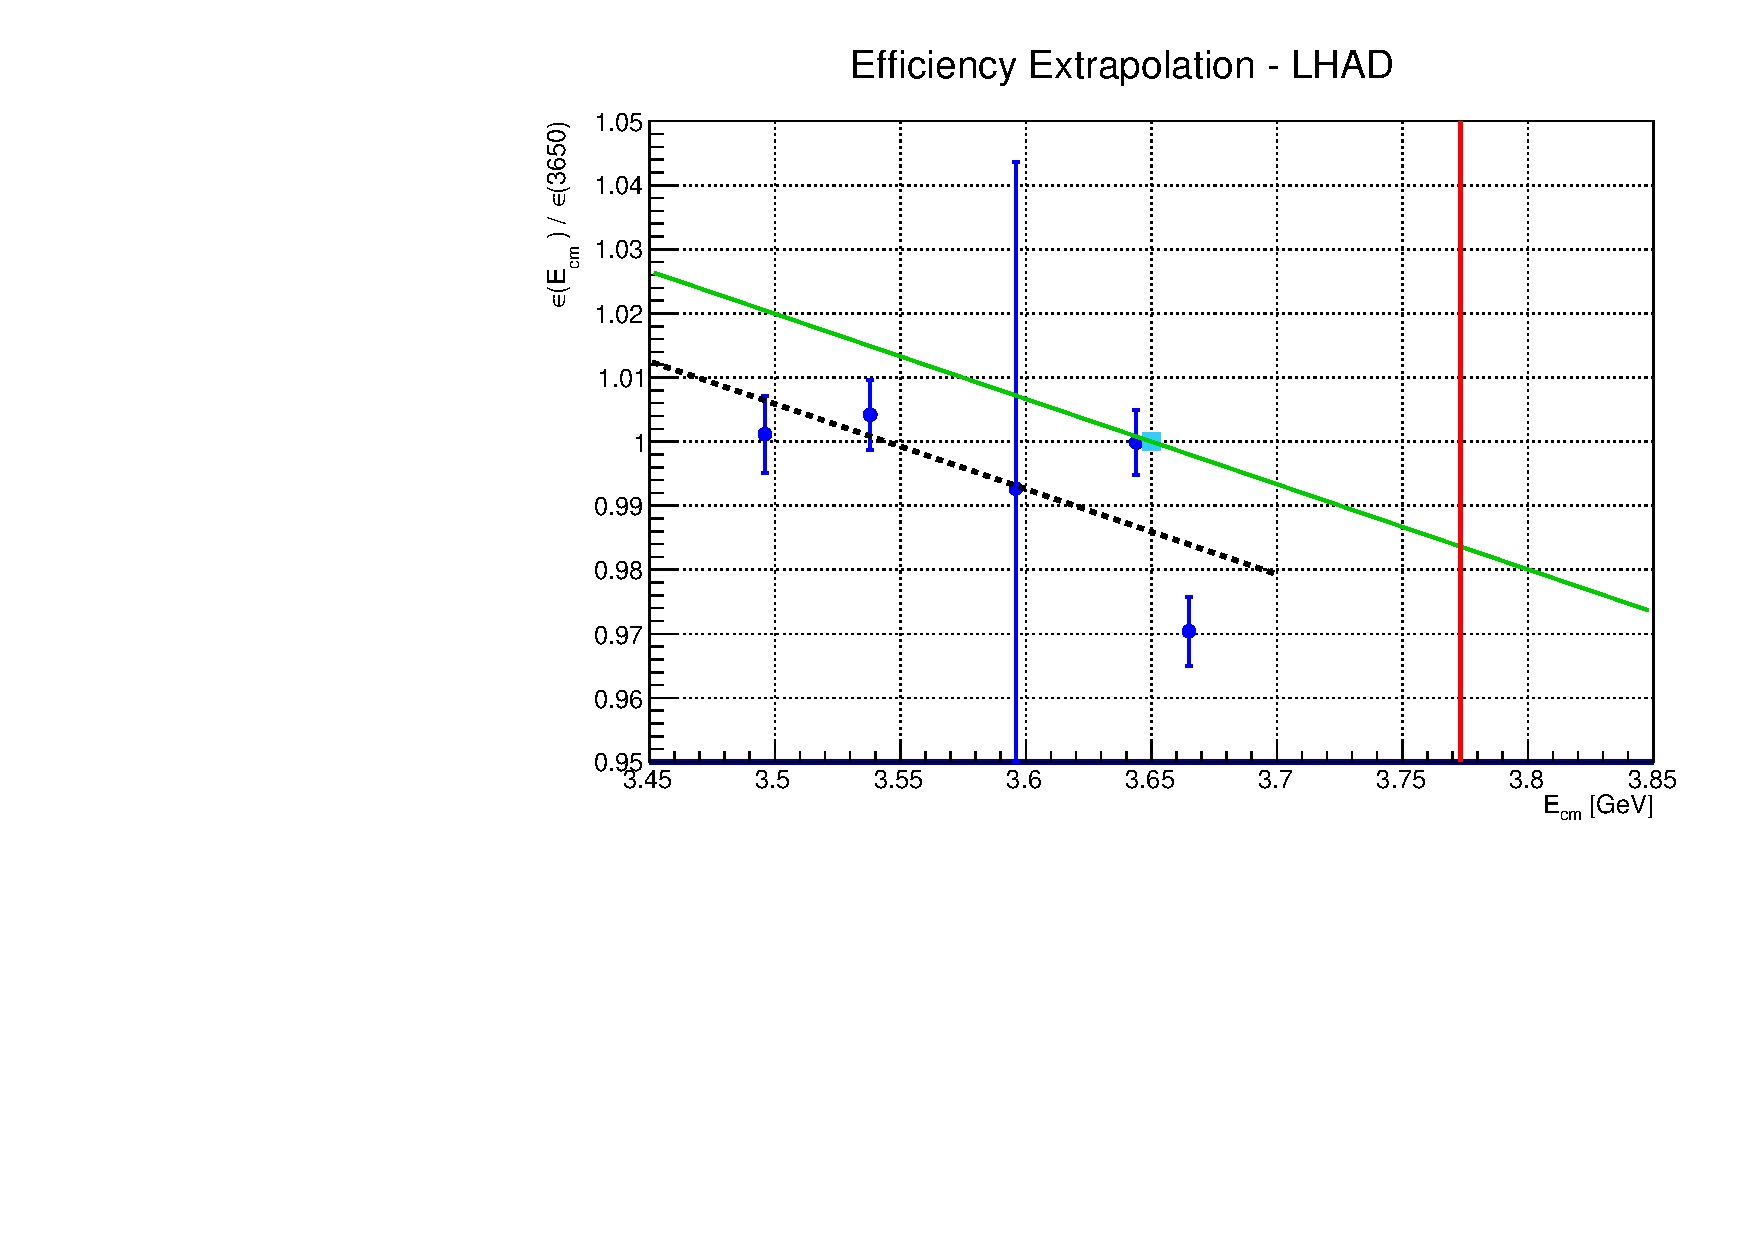
\includegraphics[scale=0.75]{figures/plots/LHAD_psip_BW.pdf}
\caption{The extrapolation for LHAD events using the new continuum data.}
{The new continuum points are fit to a linear slope (dashed black), then extrapolated to higher energies from the old continuum point (solid green). The energy of the $\psipp$ samples (solid red) is also shown.}
\label{fig:extrapolation_LHAD}
\end{figure}

\begin{figure}[H]
\centering
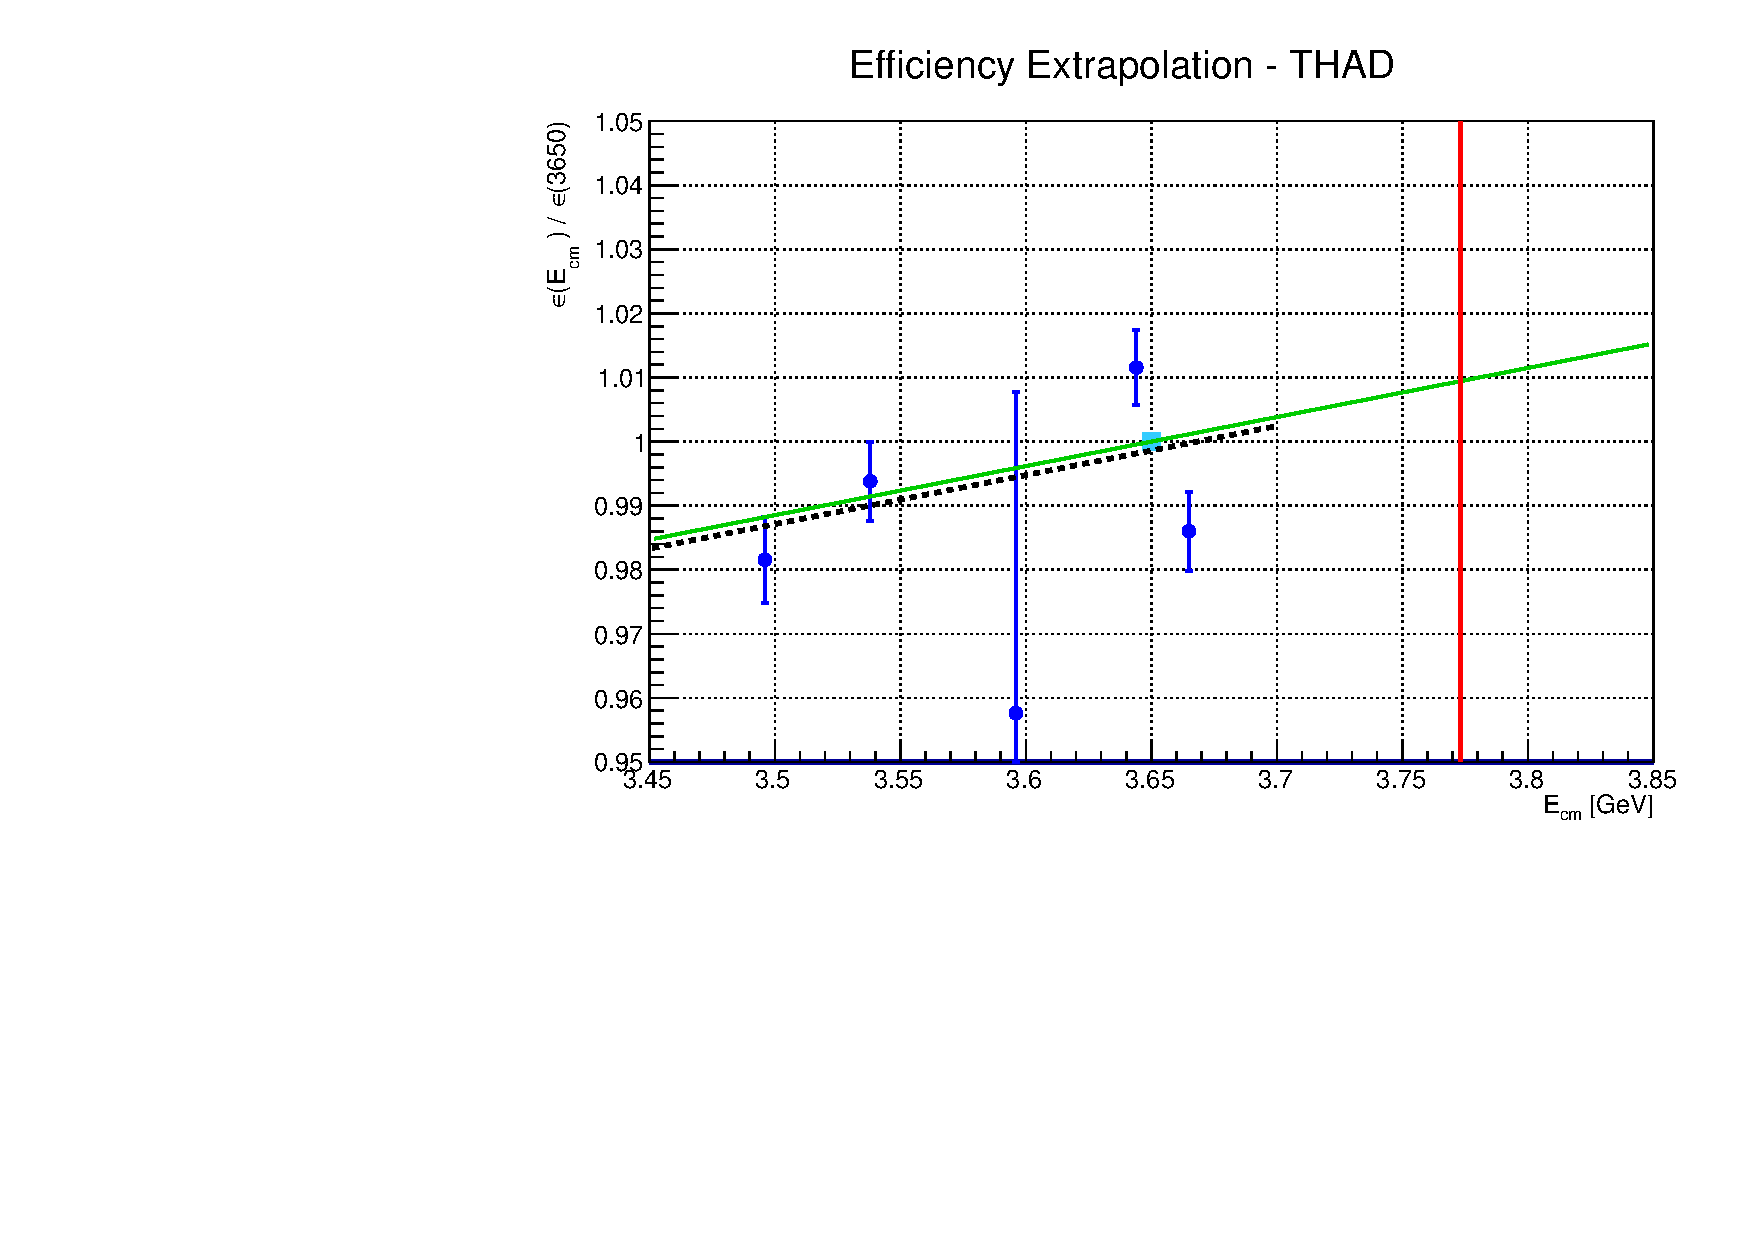
\includegraphics[scale=0.75]{figures/plots/THAD_psip_BW.pdf}
\caption{The extrapolation for THAD events using the new continuum data.}
{The new continuum points are fit to a linear slope (dashed black), then extrapolated to higher energies from the old continuum point (solid green). The energy of the $\psipp$ samples (solid red) is also shown.}
\label{fig:extrapolation_THAD}
\end{figure}



\section{$\DDbar$ Correction}
\label{sec:DDbar_correction}

\section{Results}
\label{sec:non_DDbar_results}


% Conclusion
\chapter{Conclusion}
\label{ch_conclusion}

This is where the Conclusions go!

% Bibliography
\begin{thebibliography}{99}


% -- Theory References --

\bibitem{ref:Olive:2014}
  K.A. Olive et al. (Particle Data Group),
  Chin. Phys. C, {\bf 38}, 090001 (2014).

\bibitem{ref:Wikimedia:2006}
  Wikimedia Commons.
  Standard model of elementary particles. 2006.

\bibitem{ref:Wu:1957}
  C.~S.~Wu, E.~Ambler, R.~W.~Hayward, D.~D.~Hoppes, and R.~P.~Hudson
  Phys.\ Rev.\ {\bf 105}, 1413 (1957).

\bibitem{ref:Christenson:1964}
  J.~H.~Christenson, J.~W.~Cronin, V.~L.~Fitch, and R.~Turlay
  Phys.\ Rev.\ Lett.\ {\bf 13}, 138 (1964).

\bibitem{ref:Ablikim:2013}
  M.~Ablikim et al. (BESIII Collaboration)
  Phys.\ Rev.\ Lett.\ {\bf 110}, 252001 (2013).

\bibitem{ref:Liu:2013}
  Z.~Q.~Liu et al. (Belle Collaboration)
  Phys.\ Rev.\ Lett.\ {\bf 110}, 252002 (2013).

\bibitem{ref:Aaij:2015}
  R.~Aaij et al. (LHCb Collaboration)
  Phys.\ Rev.\ Lett.\ {\bf 115}, 072001 (2015).

\bibitem{ref:Kobayashi:1973}
  M.~Kobayashi and T.~Maskawa,
  ``CP-Violation in the Renormalizable Theory of Weak Interaction''.
  Prog.\ Theor.\ Phys.\ 1973; 49 (2): 652-657. 
  [doi: 10.1143/PTP.49.652]

\bibitem{ref:Glashow:1970}
  S.~L.~Glashow, J.~Iliopoulos, and L.~Maiani
  Phys.\ Rev.\ D {\bf 2}, 1285 (1970).

\bibitem{ref:Pontecorvo:1957}
  B.~Pontecorvo. (1957).
  ``Inverse beta processes and nonconservation of lepton charge''.
  Zhurnal Éksperimental’noĭ i Teoreticheskoĭ Fiziki.  {\bf 34}: 247.
  reproduced and translated in Soviet Physics JETP. 7: 172. 1958.

\bibitem{ref:Maki:1962}
  Z.~Maki, M.~Nakagawa, S.~Sakata. (1962).
  ``Remarks on the Unified Model of Elementary Particles''.
  Progress of Theoretical Physics. {\bf 28}: 870.

\bibitem{ref:Rosner:2001} 
  J.~L.~Rosner,
  %``Charmless final states and S D wave mixing in the psi-prime- prime,''
  Phys.\ Rev.\ D {\bf 64}, 094002 (2001)
  [hep-ph/0105327].
  %%CITATION = HEP-PH/0105327;%%

\bibitem{ref:Rosner:2004} 
  J.~L.~Rosner,
  %``Psi'' decays to charmless final states,''
  Annals Phys.\  {\bf 319}, 1 (2005)
  [hep-ph/0411003].
  %%CITATION = HEP-PH/0411003;%%

\bibitem{ref:Okubo:1963} 
  S.~Okubo,
  %``Phi meson and unitary symmetry model,''
  Phys.\ Lett.\  {\bf 5}, 165 (1963).
  %%CITATION = PHLTA,5,165;%%

\bibitem{ref:Zweig:1964} 
  G.~Zweig,
  %``An SU(3) model for strong interaction symmetry and its breaking. Version 2,''
  Developments in the Quark Theory of Hadrons, Volume 1. Edited by D. Lichtenberg and S. Rosen. pp. 22-101

\bibitem{ref:Iizuka:1966} 
  J.~Iizuka, K.~Okada and O.~Shito,
  %``Systematics and phenomenology of boson mass levels. 3.,''
  Prog.\ Theor.\ Phys.\  {\bf 35}, 1061 (1966).
  %%CITATION = PTPKA,35,1061;%%

\bibitem{ref:Kuraev:1985}
  E.~A.~Kuraev and V.~S.~Fadin,
  %``On Radiative Corrections to e+ e- Single Photon Annihilation at High-Energy,''
  Sov.\ J.\ Nucl.\ Phys.\  {\bf 41}, 466 (1985)
  [Yad.\ Fiz.\  {\bf 41}, 733 (1985)].
  %%CITATION = SJNCA,41,466;%%

\bibitem{ref:Anashin:2012}
  V.~V.~Anashin {\it et al.},
  %``Measurement of \psi(3770) parameters,''
  Phys.\ Lett.\ B {\bf 711}, 292 (2012)
  [arXiv:1109.4205 [hep-ex]].
  %%CITATION = ARXIV:1109.4205;%%

\bibitem{ref:Blatt:1952}
  J.~M.~Blatt and V.~F.~Weisskopf,
  Theoretical Nuclear Physics, Wiley, New York, (1952).


% -- Detector References --

\bibitem{ref:Ablikim:2009} 
  M.~Ablikim {\it et al.}  [BESIII Collaboration],
  %``Design and Construction of the BESIII Detector,''
  Nucl.\ Instrum.\ Meth.\ A {\bf 614}, 345 (2010)
  [arXiv:0911.4960 [physics.ins-det]].
  %%CITATION = ARXIV:0911.4960;%%

\bibitem{ref:Jackson:1999}
  J.~D.~Jackson.
  {\it Classical Electrodynamics (3rd ed.)}.
  Wiley. (Section 13.2)
 
\bibitem{ref:Li:2006}
  W.~Li, {\it et al.},
  Proc.\ Int.\ Conf.\ Comput.\ High Energy and Nucl.\ Phys.\ 225 (2006).

\bibitem{ref:SLC5}
  See \url{http://linux.web.cern.ch/linux/scientific5}.

\bibitem{ref:Barrand:2001} 
  G.~Barrand, I.~Belyaev, P.~Binko, M.~Cattaneo, R.~Chytracek, G.~Corti, M.~Frank and G.~Gracia {\it et al.},
  %``GAUDI - A software architecture and framework for building HEP data processing applications,''
  Comput.\ Phys.\ Commun.\  {\bf 140}, 45 (2001).
  %%CITATION = CPHCB,140,45;%%

\bibitem{ref:Arnault:2000} 
  C.~Arnault, ``CMT: A software configuration management tool,'' (2000).

\bibitem{ref:ROOT}
  See \url{http://root.cern.ch}.

\bibitem{ref:Agostinelli:2003}
  S.~Agostinelli, {\it et al.}, Nucl.\ Instr.\ and Meth.\ {\bf 506}, (3), 250 (2003);
  J.~Allison, {\it et al.}, IEEE Trans.\ Nucl.\ Sci.\ NS {\bf 53} (1), 270 (2006);
  See \url{http://www.geant4.org/geant4}.

\bibitem{ref:Jadach:2000} S. Jadach , B. F. L. Ward and Z. Was,
  Comp. Phys. Commun. {\bf 130}, 260 (2000); S. Jadach, B. F. L. Ward
  and  Z. Was, Phys. Rev. D {\bf 63}, 113009~(2001).

\bibitem{ref:Jadach:1993} 
  S.~Jadach, Z.~Was, R.~Decker and J.~H.~Kuhn,
  %``The tau decay library TAUOLA: Version 2.4,''
  Comput.\ Phys.\ Commun.\  {\bf 76}, 361 (1993).
  %%CITATION = CPHCB,76,361;%%

\bibitem{ref:PYTHIA}
  See \url{http://home.thep.lu.se/\~torbjorn/Pythia.html}.

\bibitem{ref:Lange:2001} 
  D.J.~Lange,
  Nucl.\ Instrum.\ Meth.\ A {\bf 462},
  152~(2001).

\bibitem{ref:Ping:2008}
  R. G. Ping, Chinese Physics C {\bf 32}, 8~(2008).

\bibitem{ref:Barberio:1991} 
  E.~Barberio, B.~van Eijk and Z.~Was,
  %``PHOTOS: A Universal Monte Carlo for QED radiative corrections in decays,''
  Comput.\ Phys.\ Commun.\  {\bf 66}, 115 (1991).
  %%CITATION = CPHCB,66,115;%%

\bibitem{ref:Chen:2000}
  J.~C.~Chen, G.~S.~Huang, X.~R.~Qi, D.~H.~Zhang and Y.~S.~Zhu,
  %``Event generator for J / psi and psi (2S) decay,''
  Phys.\ Rev.\ D {\bf 62}, 034003 (2000).

\bibitem{ref:Bonneau:1971}
  G.~Bonneau and F.~Martin,
  Nucl.\ Phys.\ B {\bf 27}, 381 (1971).

\bibitem{ref:Carloni:2004}
  C.M.~Carloni Calame, G.~Montagna, O.~Nicrosini, F.~Piccinini,
  Nucl.\ Phys.\ Proc.\ Suppl.\ {\bf 131} 48-55 (2004).

\bibitem{ref:MySQL}
  See \url{http://www.mysql.com/about}.

\bibitem{ref:Baltrusaitis:1986}
  R.~M.~Baltrusaitis {\it et al.}  [MARK-III Collaboration],
  %``Direct Measurements Of Charmed $D$ Meson Hadronic Branching Fractions,''
  Phys.\ Rev.\ Lett.\  {\bf 56}, 2140 (1986).
  %%CITATION = PRLTA,56,2140;%%

\bibitem{ref:Adler:1988}
  J.~Adler {\it et al.}  [MARK-III Collaboration],
  %``A Reanalysis Of Charmed $D$ Meson Branching Fractions,''
  Phys.\ Rev.\ Lett.\  {\bf 60}, 89 (1988).
  %%CITATION = PRLTA,60,89;%%


\bibitem{ref:Toth:2014}
    D.~Toth. (2014).
    ``Measurement of Non-$\DDbar$ Decays of the $\psipp$ Resonance at BESIII''.

\bibitem{ref:Dong:2014}
  L.~Dong,
  ``Center-of-mass beam energy calibration for psi(3770) data with BOSS 6.6.4,''
  BESIII-doc-284-v6 (2014).

\bibitem{ref:Hafner:2015}
  A.~Hafner,
  ``Luminosity Measurement for the $\psipp$ data at BESIII,''
  BESIII-doc-406-v2 (2015).


\bibitem{ref:Asner:2008}
  D.~M.~Asner and W.~M.~Sun,
  Phys. Rev. D, {\bf 77}, 019901 (2008).

\bibitem{ref:HFAG:2015}
  HFAG 2015 ($CPV$-Allowed)
  [http://www.slac.stanford.edu/xorg/hfag/charm/CHARM15/results\_mix\_cpv.html]

\bibitem{ref:Evans:2016}
  T.~Evans et al., Physics Letters B 757 (2016) 520–527.
\bibitem{ref:Ablikim:2013b}
  M.~Ablikim et al. [BESIII Collaboration], 
  Chin. Phys. C, {\bf 37}, 12 (2013):12300.

\bibitem{ref:Rong:2015}
  G.~Rong et. al, 
  ``Measurements of Branching Fractions and Form Factors for $D^0 \to K^-e ^+\nu_e,~\pi^-e^+\nu_e$ Decays'',
  BESIII-doc-125-v3 (2015).

\bibitem{ref:Ke:2015}
  B.~C.~Ke et al. [Carnegie Mellon University], 
  ``$\piO$ Reconstruction Efficiency'',
  BESIII-doc-446-v4 (2015).

\bibitem{ref:Ma:2014}
  T.~Ma ,
  ``Determination of $\Ks$ Systematics'',
  BESIII-doc-125-v3 (2014).


\end{thebibliography}

% \bibliography{references}

% Appendices
\appendix
\chapter{Glossary and Acronyms}
\label{app_glossary}

Care has been taken in this thesis to minimize the use of jargon and
acronyms, but this cannot always be achieved.  This appendix defines
jargon terms in a glossary, and contains a table of acronyms and their
meaning.

% Glossary {{{
\section{Glossary}
\label{sec_glossary}

\begin{itemize}

\item \textbf{Cosmic-Ray Muon} (\textbf{CR $\mu$}) -- A muon coming from
the abundant energetic particles originating outside of the Earth's
atmosphere.

\end{itemize}


% Acronyms {{{
\section{Acronyms}
\label{sec_acronym}

% Table formatting

% Heading for the first page
\begin{longtable}{p{0.25\textwidth} p{0.75\textwidth}}
\caption{Acronyms} \label{tab:acronyms} \\

\toprule
Acronym & Meaning \\
\midrule
\endfirsthead

% Heading for all subsequent pages
\multicolumn{2}{l}{\textit{\tablename\ \thetable{} -- Continued from previous page}} \\
\toprule
Acronym & Meaning \\
\midrule
\endhead

% Footer for each page that wraps over to the next
\multicolumn{2}{r}{\textit{Continued on next page}} \\
\bottomrule
\endfoot

% Footer for the end of the table
\bottomrule
\endlastfoot

% End table formatting

CR$\mu$ & Cosmic-Ray Muon \\

\end{longtable}

\chapter{$\DO$ Signal Fits}
\label{app:D0_signal_fits}

\begin{figure}[h]

\begin{subfigure}[c]{0.99\textwidth}
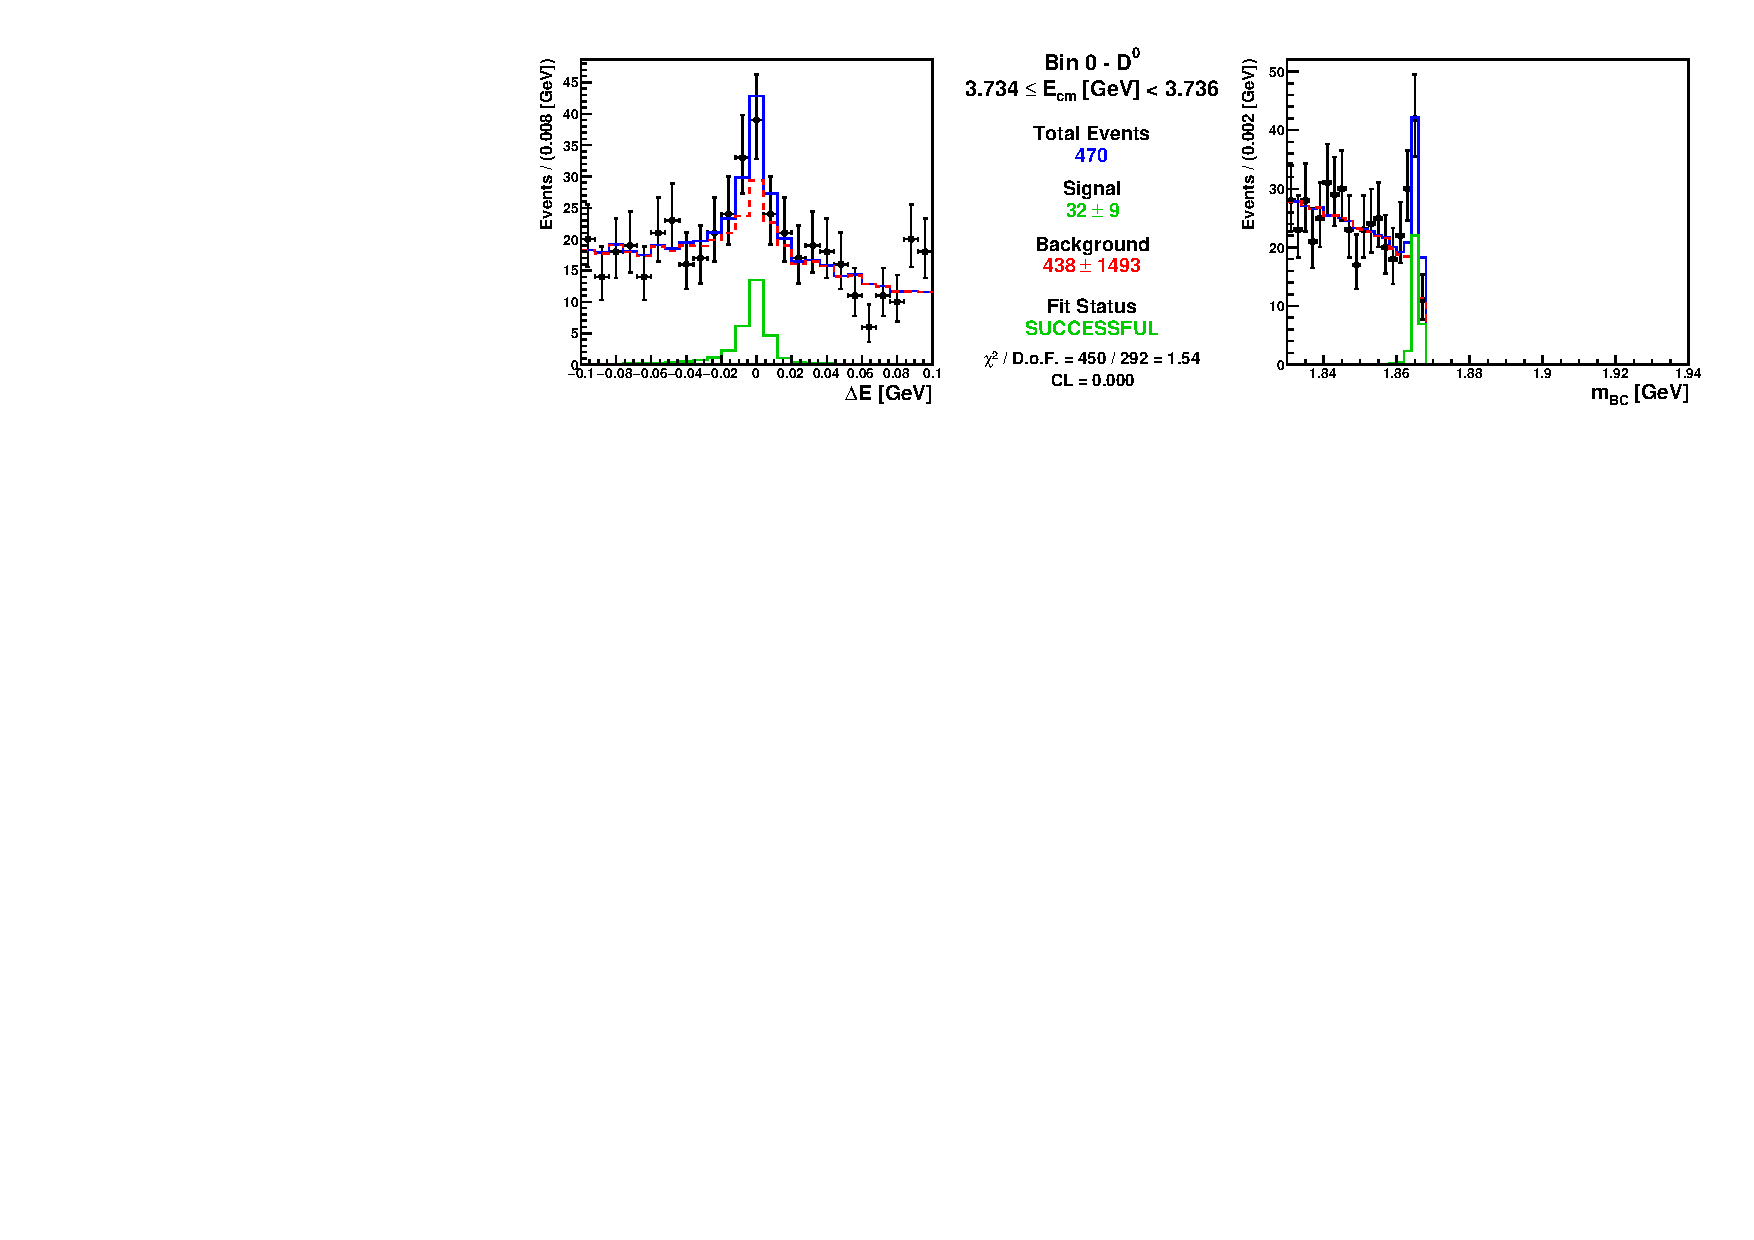
\includegraphics[width=\textwidth]{figures/plots/fit_results/D0_bin_00.pdf}
\caption*{Signal Fit - $\DO$ Bin 0}
\end{subfigure}

\vspace{5pt}

\begin{subfigure}[c]{0.99\textwidth}
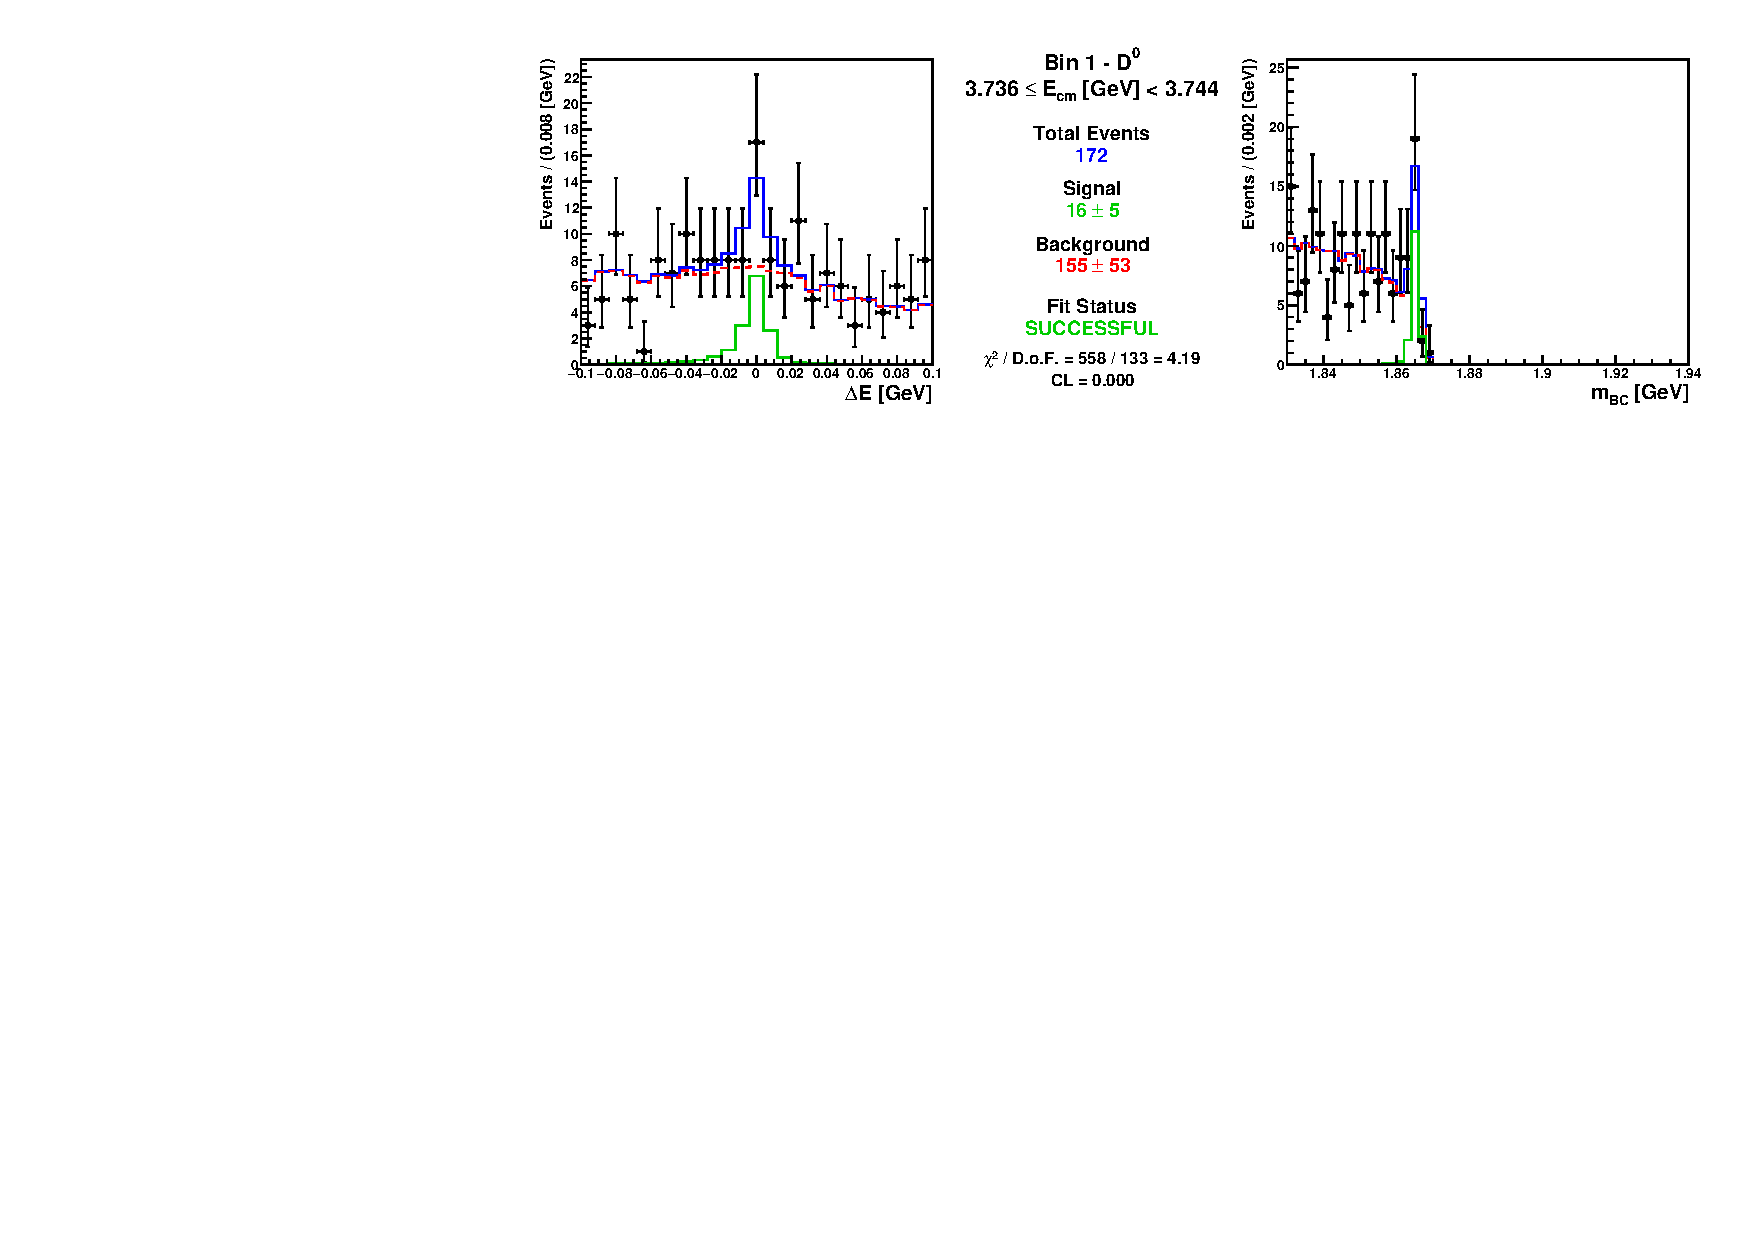
\includegraphics[width=\textwidth]{figures/plots/fit_results/D0_bin_01.pdf}
\caption*{Signal Fit - $\DO$ Bin 1}
\end{subfigure}

\caption{Signal Fitting Plots for $\DO$ Bins 0 - 1.}
\label{fig:DO_plots_0_2}

\end{figure}


\begin{figure}[h]

\begin{subfigure}[c]{0.99\textwidth}
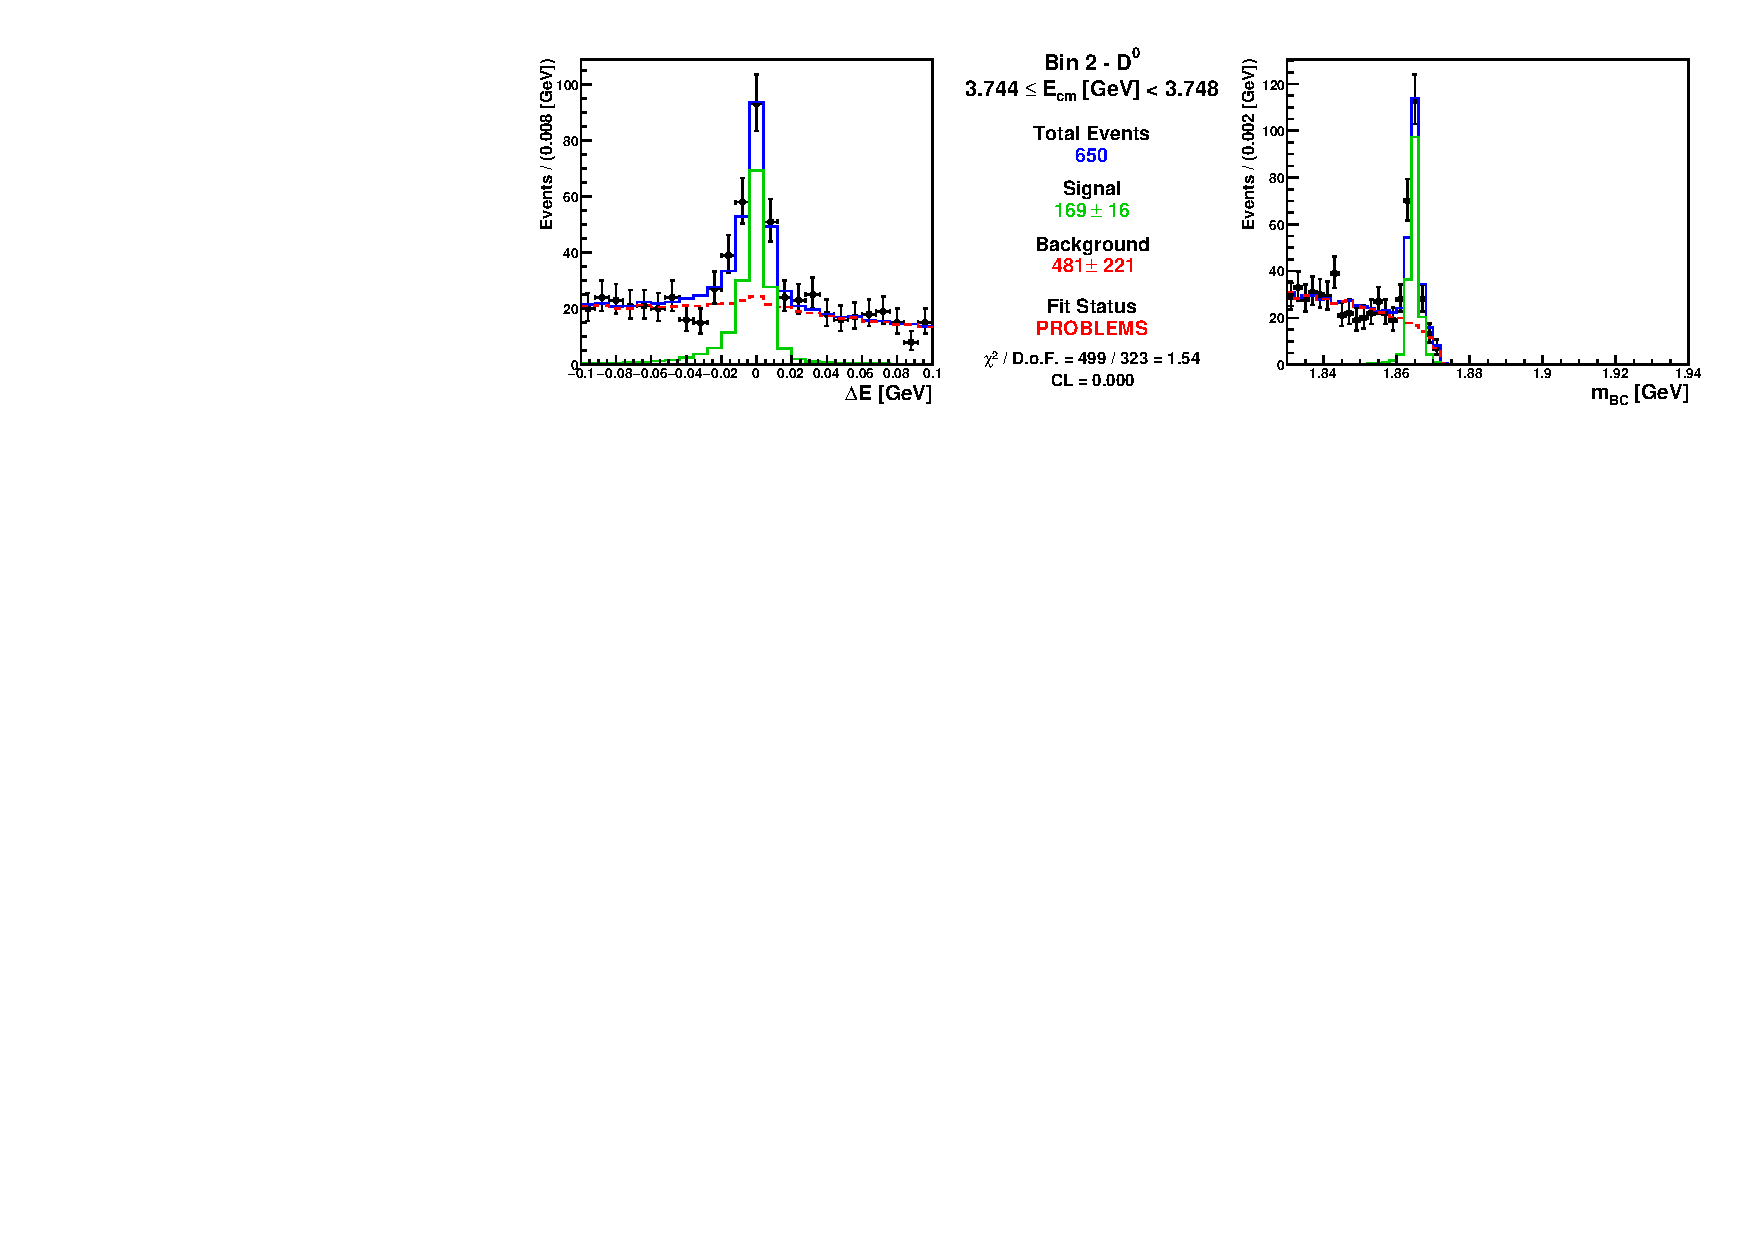
\includegraphics[width=\textwidth]{figures/plots/fit_results/D0_bin_02.pdf}
\caption*{Signal Fit - $\DO$ Bin 2}
\end{subfigure}

\vspace{5pt}

\begin{subfigure}[c]{0.99\textwidth}
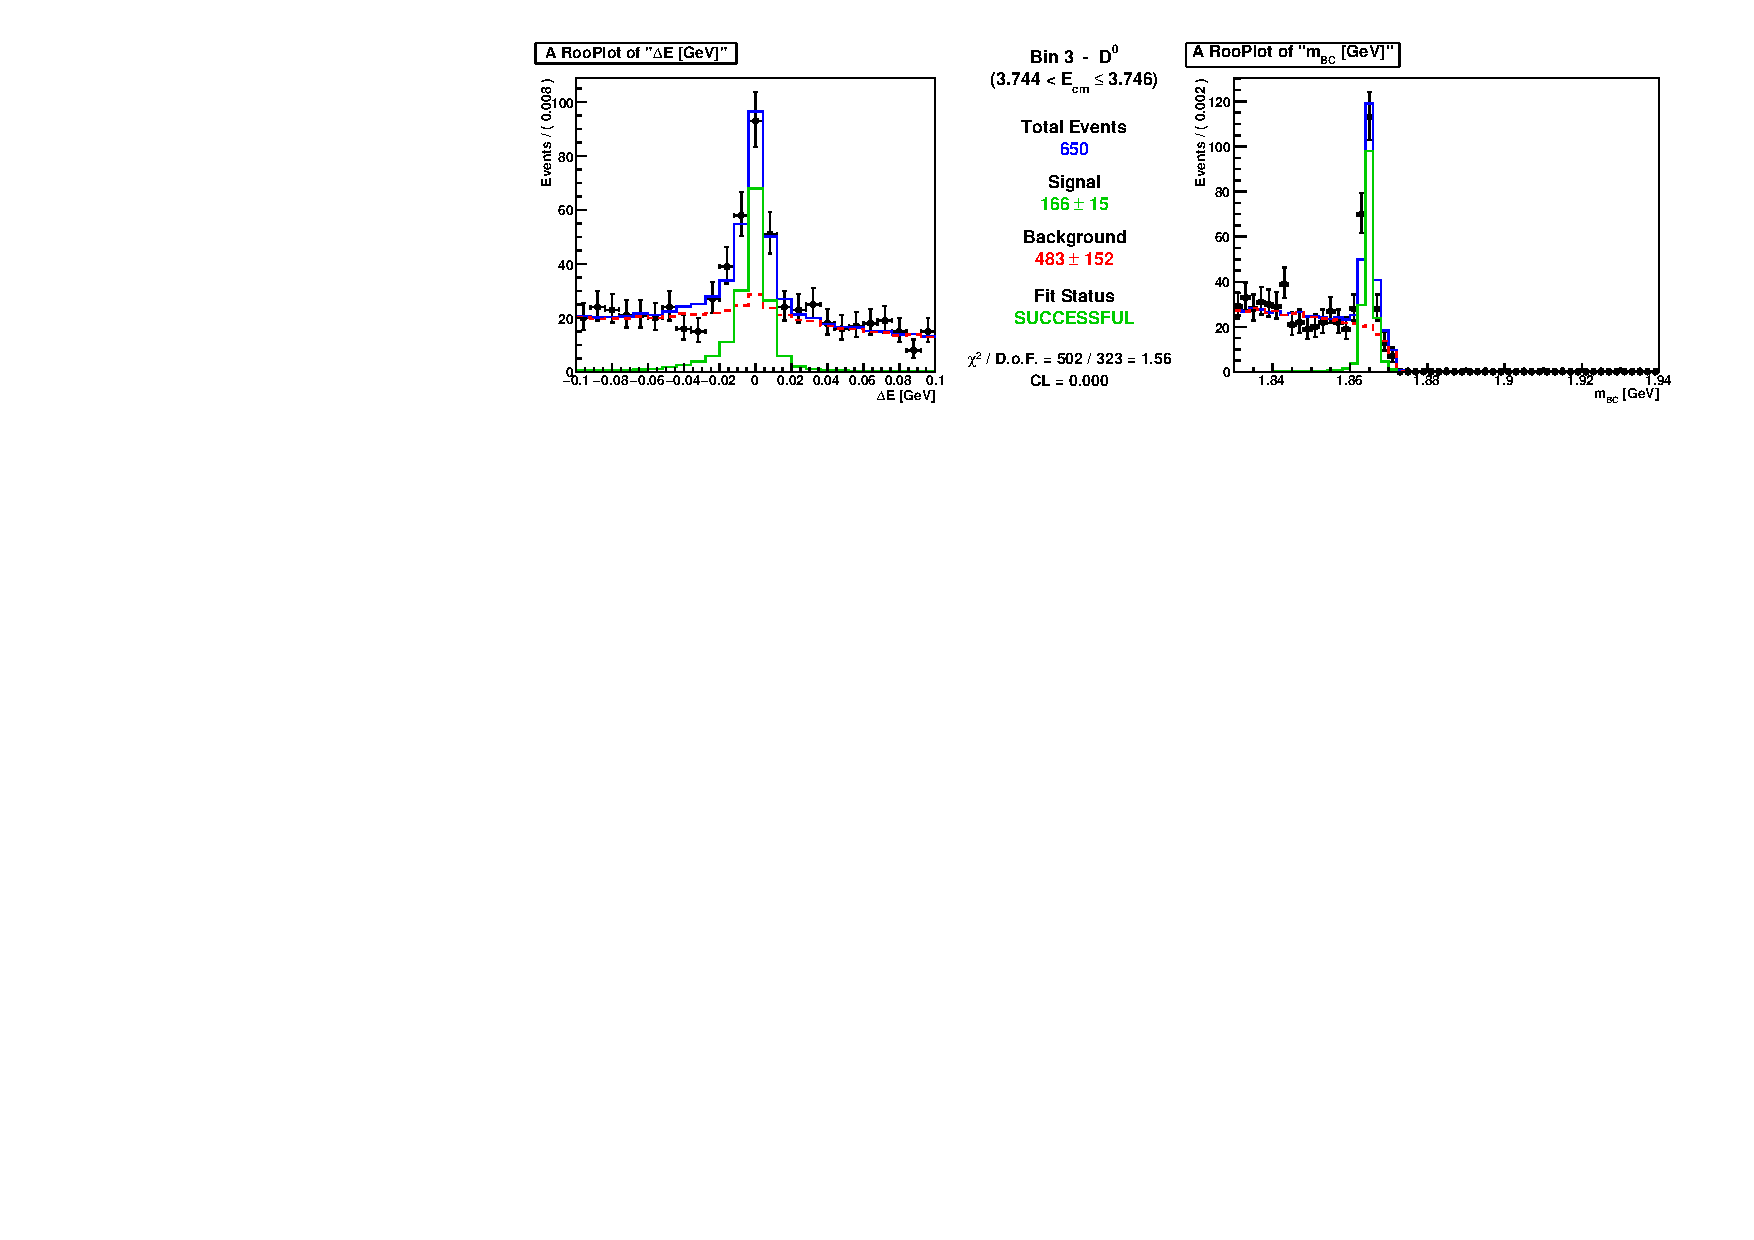
\includegraphics[width=\textwidth]{figures/plots/fit_results/D0_bin_03.pdf}
\caption*{Signal Fit - $\DO$ Bin 3}
\end{subfigure}

\vspace{5pt}

\begin{subfigure}[c]{0.99\textwidth}
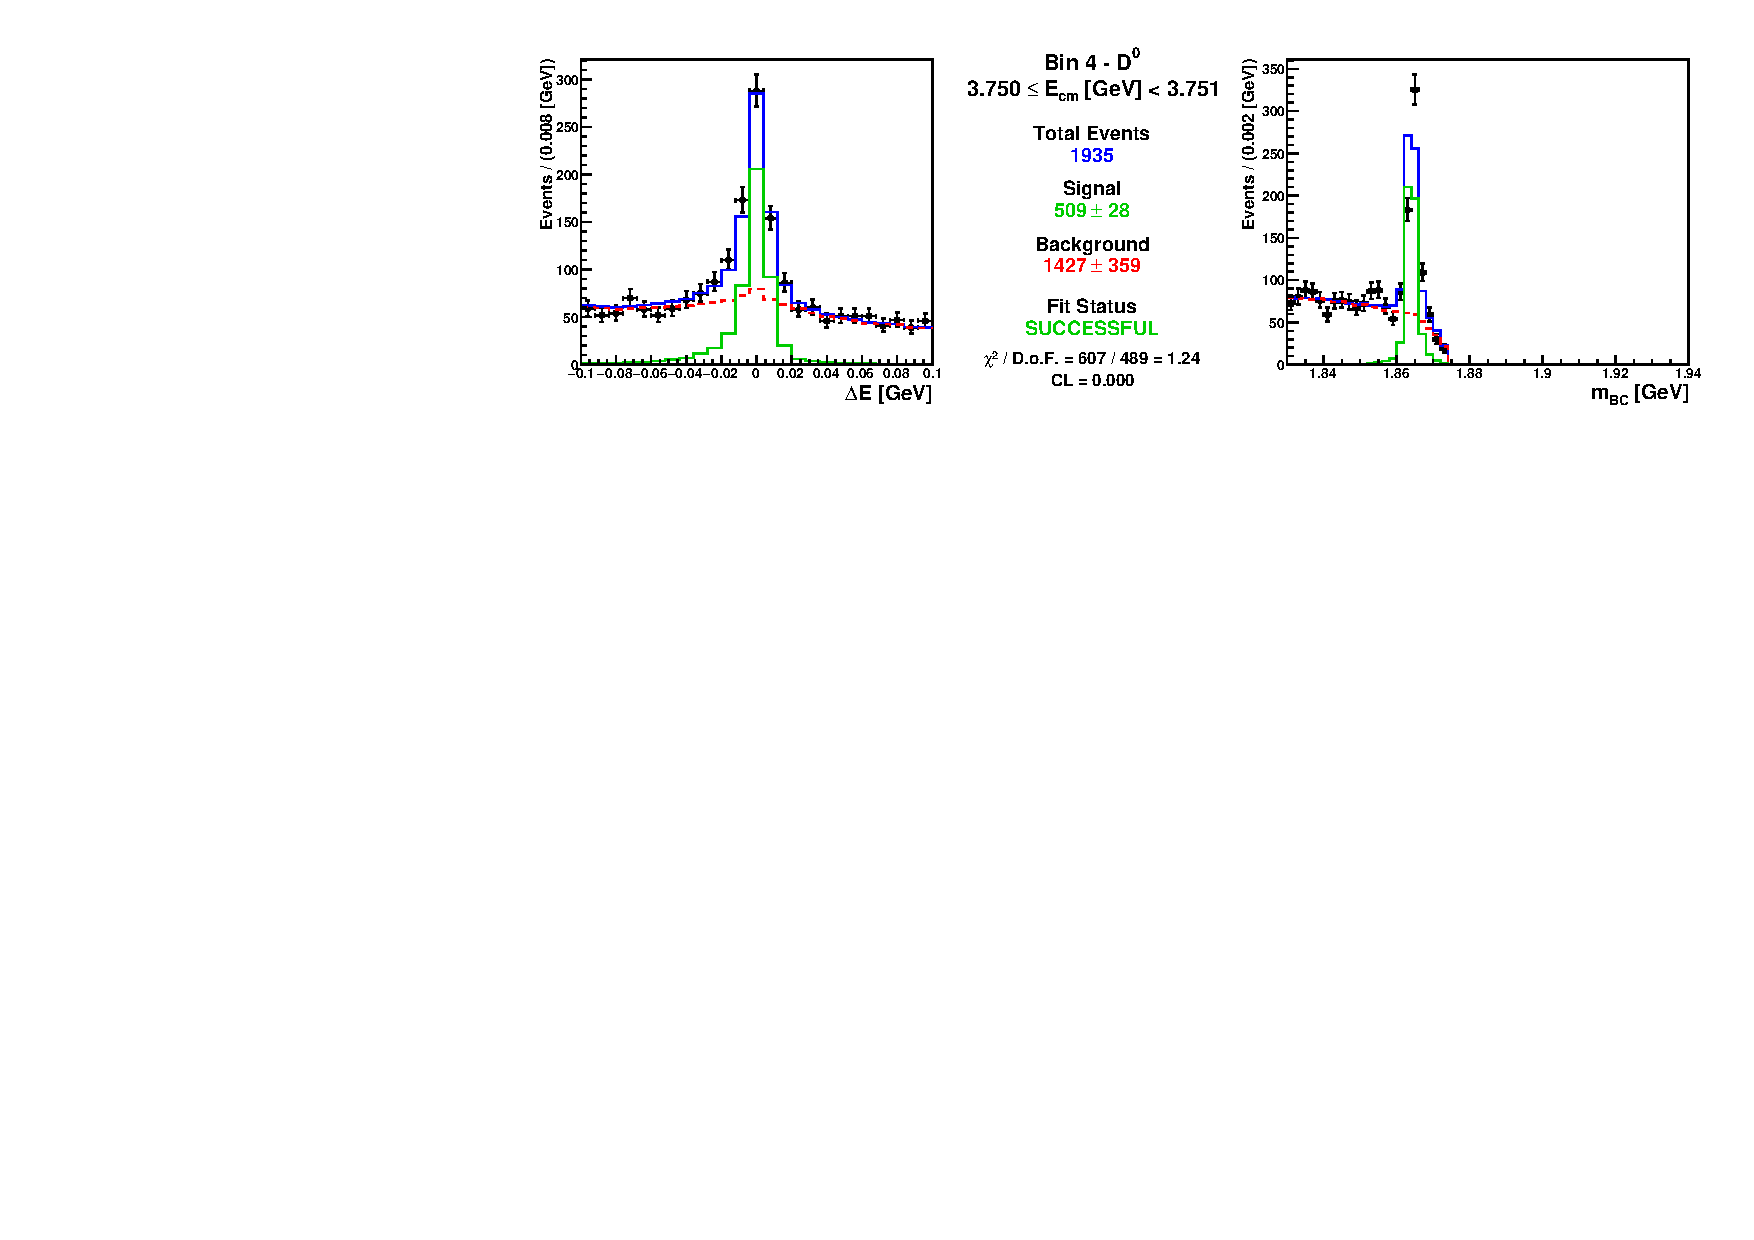
\includegraphics[width=\textwidth]{figures/plots/fit_results/D0_bin_04.pdf}
\caption*{Signal Fit - $\DO$ Bin 4}
\end{subfigure}

\vspace{5pt}

\begin{subfigure}[c]{0.99\textwidth}
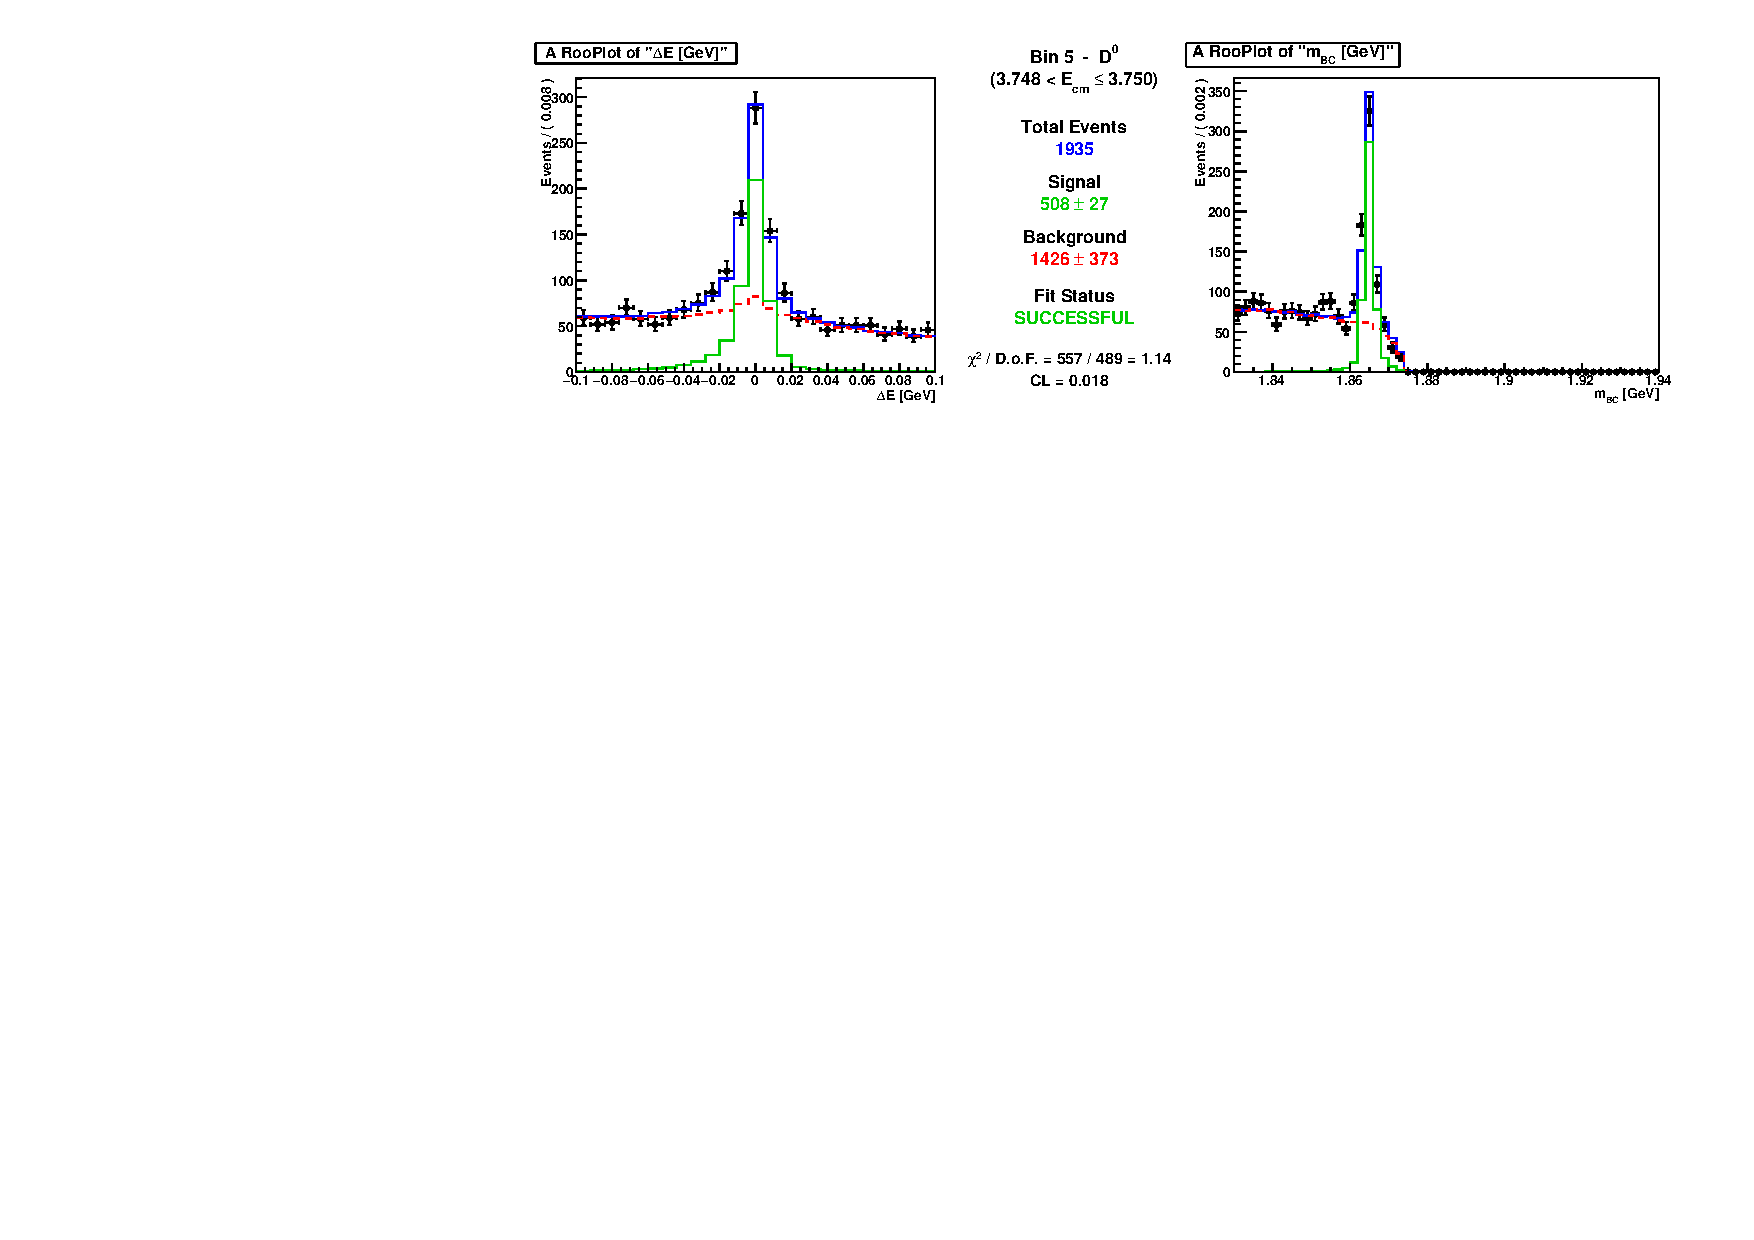
\includegraphics[width=\textwidth]{figures/plots/fit_results/D0_bin_05.pdf}
\caption*{Signal Fit - $\DO$ Bin 5}
\end{subfigure}

\caption{Signal Fitting Plots for $\DO$ Bins 2 - 5.}
\label{fig:DO_plots_2_5}

\end{figure}


\begin{figure}[h]

\begin{subfigure}[c]{0.99\textwidth}
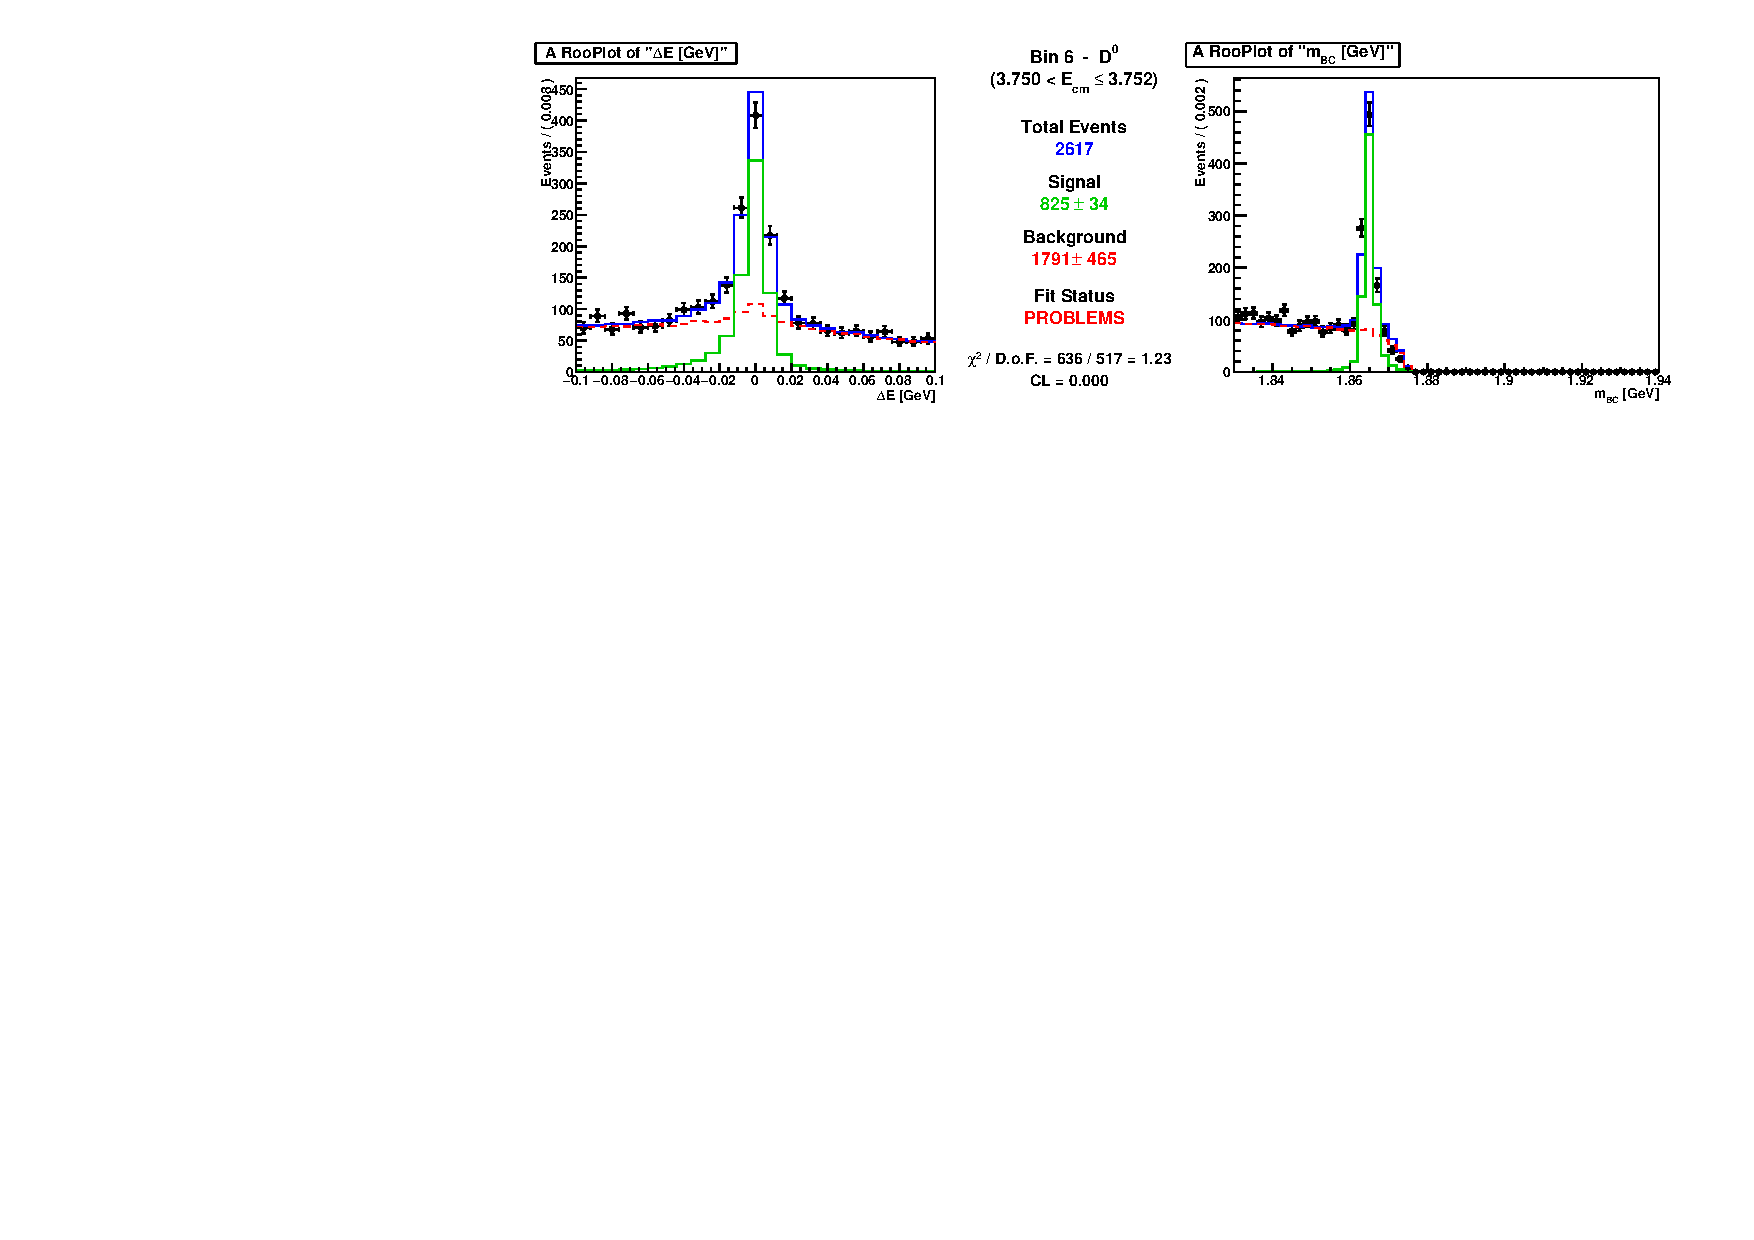
\includegraphics[width=\textwidth]{figures/plots/fit_results/D0_bin_06.pdf}
\caption*{Signal Fit - $\DO$ Bin 6}
\end{subfigure}

\vspace{5pt}

\begin{subfigure}[c]{0.99\textwidth}
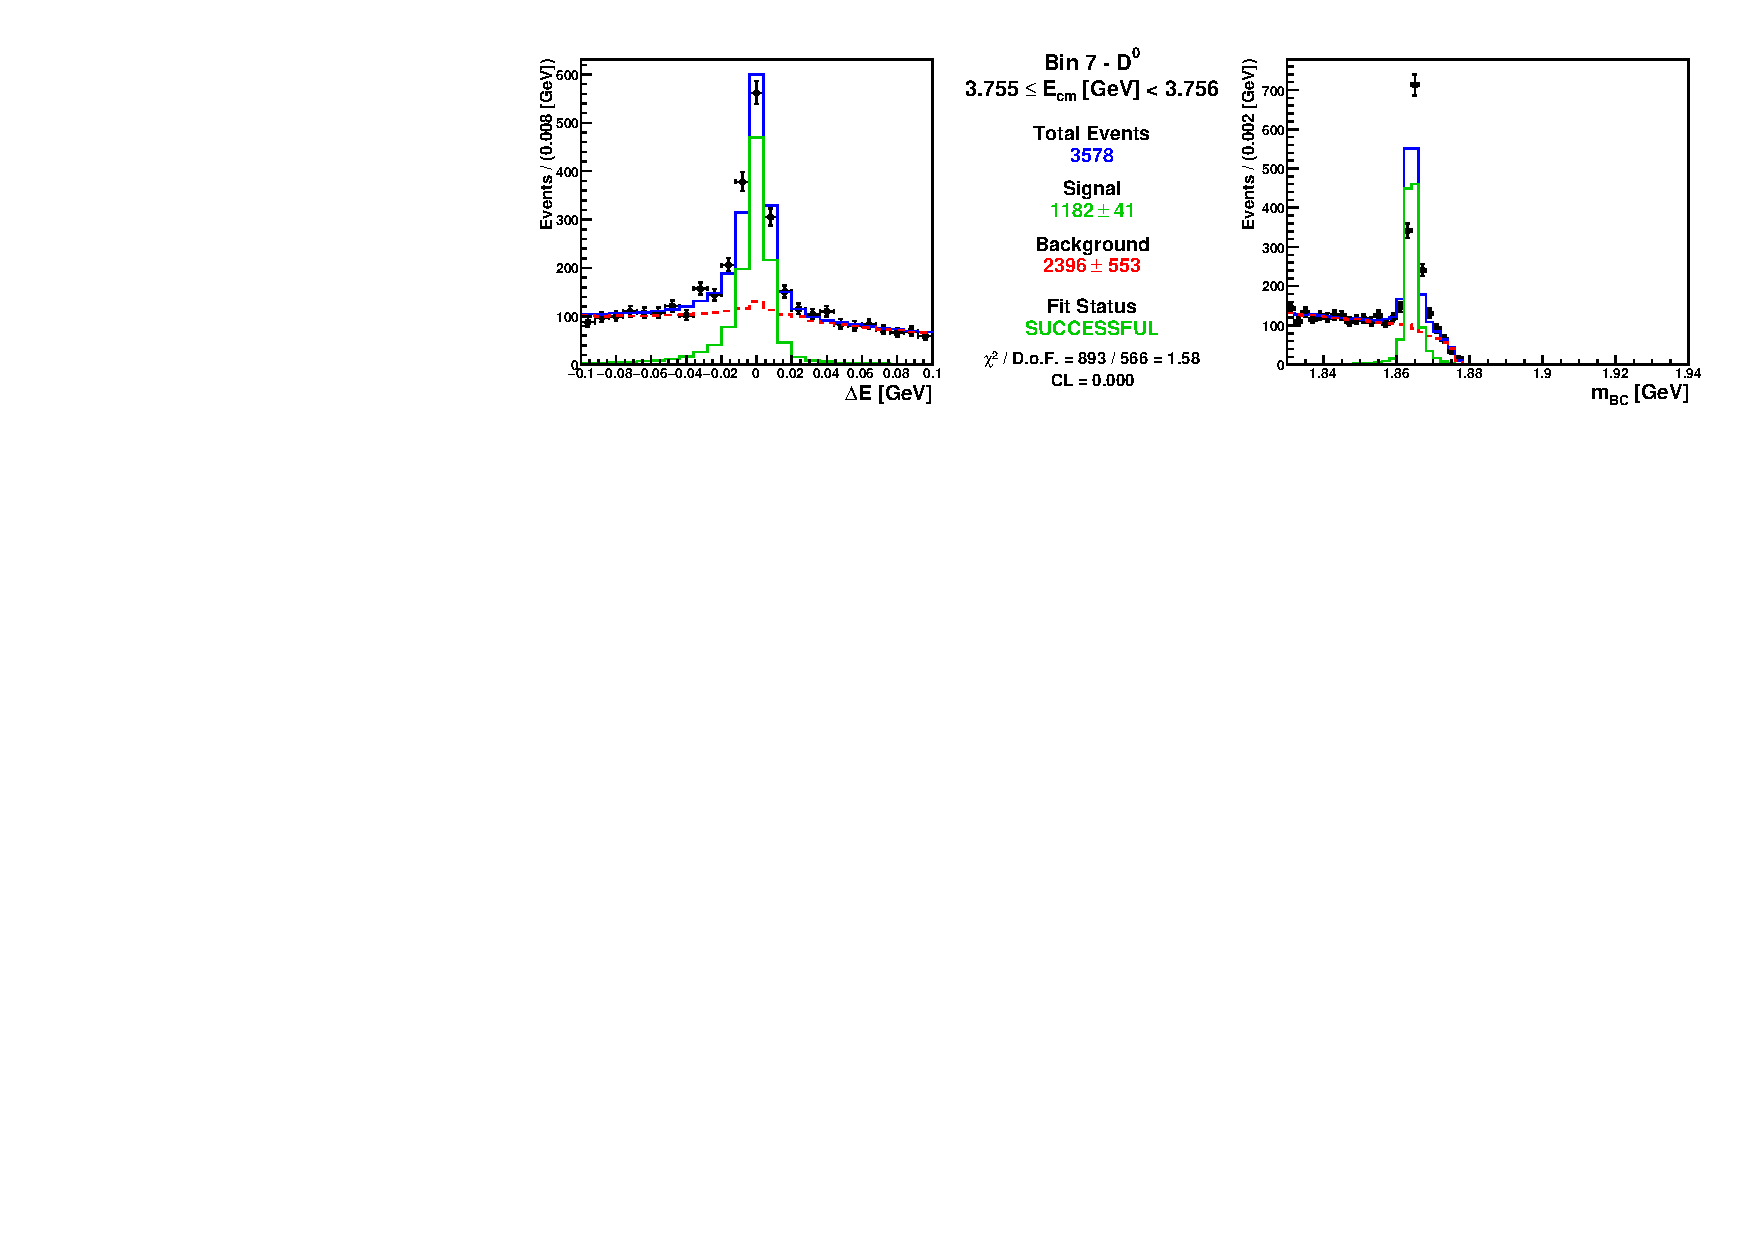
\includegraphics[width=\textwidth]{figures/plots/fit_results/D0_bin_07.pdf}
\caption*{Signal Fit - $\DO$ Bin 7}
\end{subfigure}

\vspace{5pt}

\begin{subfigure}[c]{0.99\textwidth}
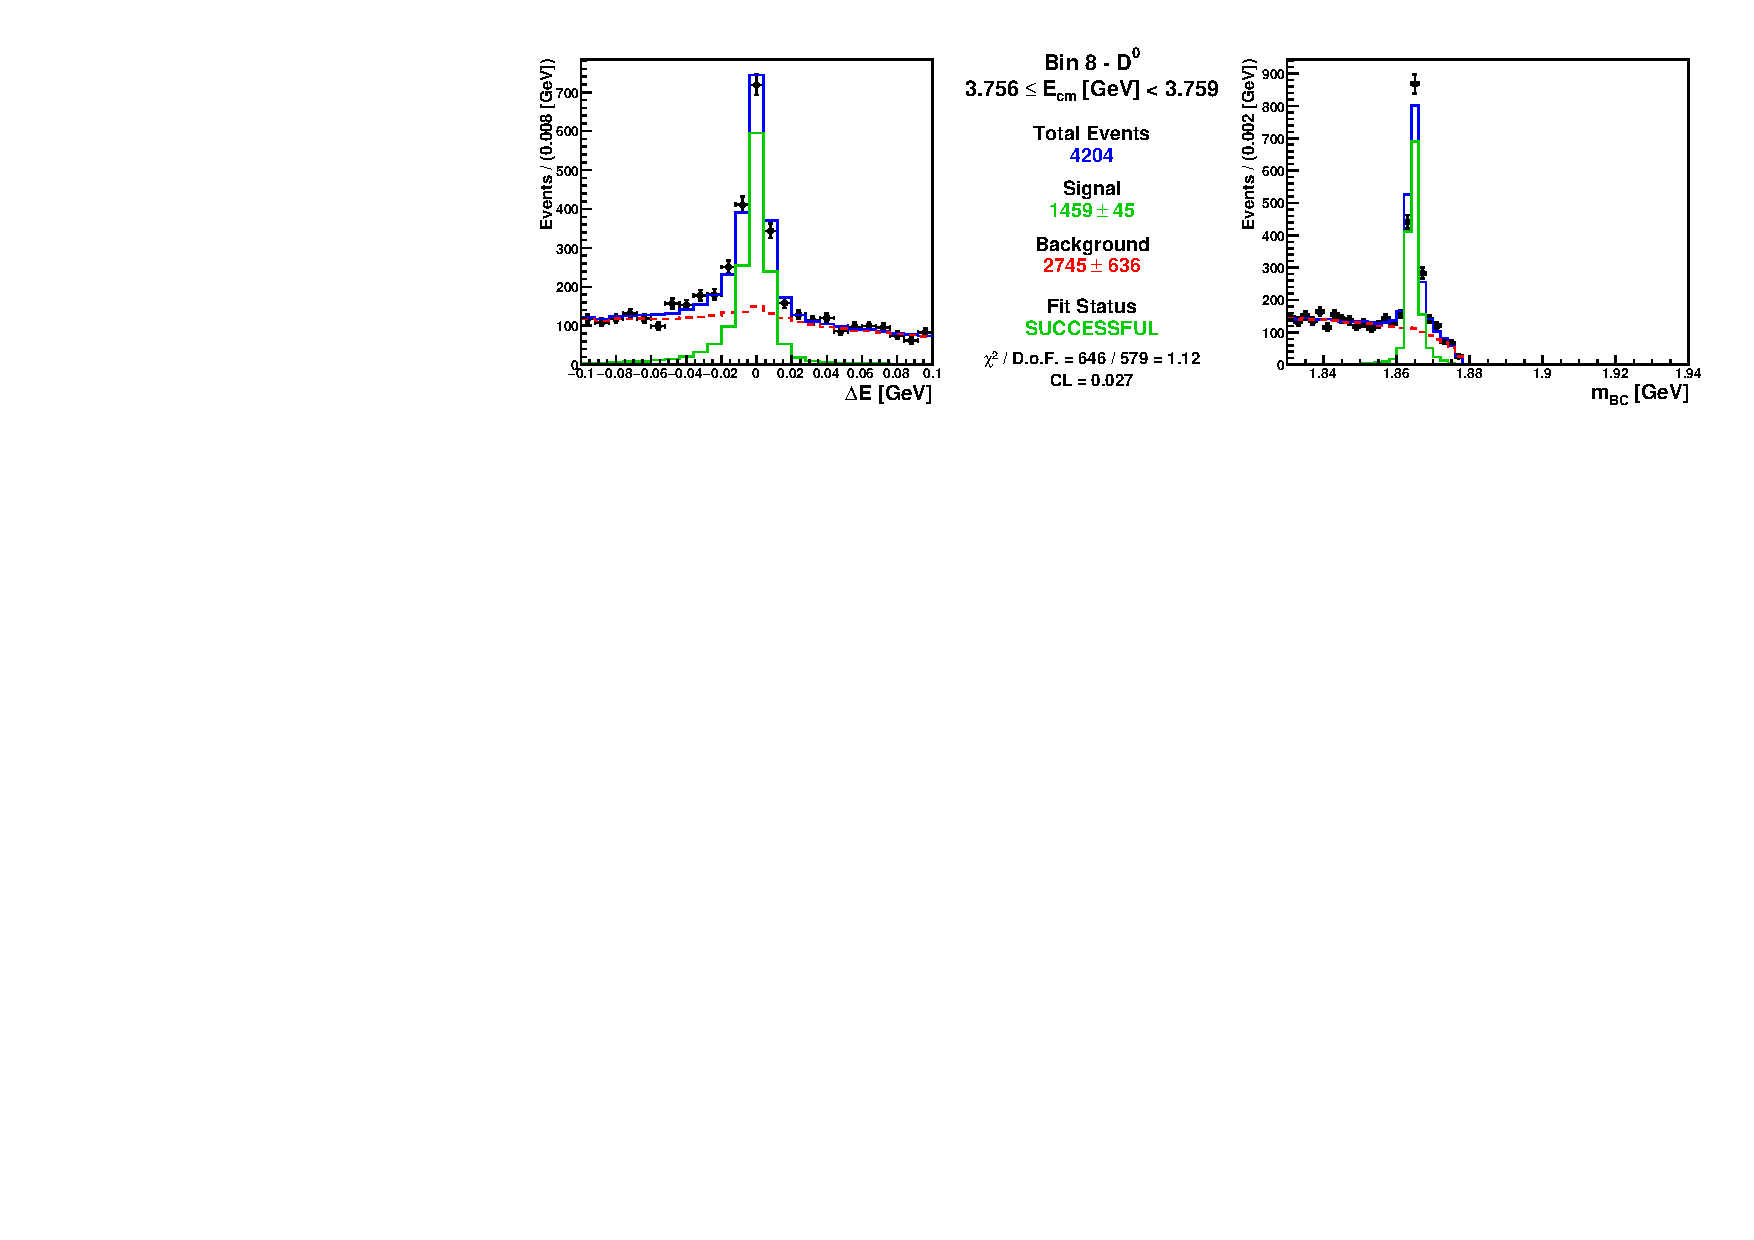
\includegraphics[width=\textwidth]{figures/plots/fit_results/D0_bin_08.pdf}
\caption*{Signal Fit - $\DO$ Bin 8}
\end{subfigure}

\vspace{5pt}

\begin{subfigure}[c]{0.99\textwidth}
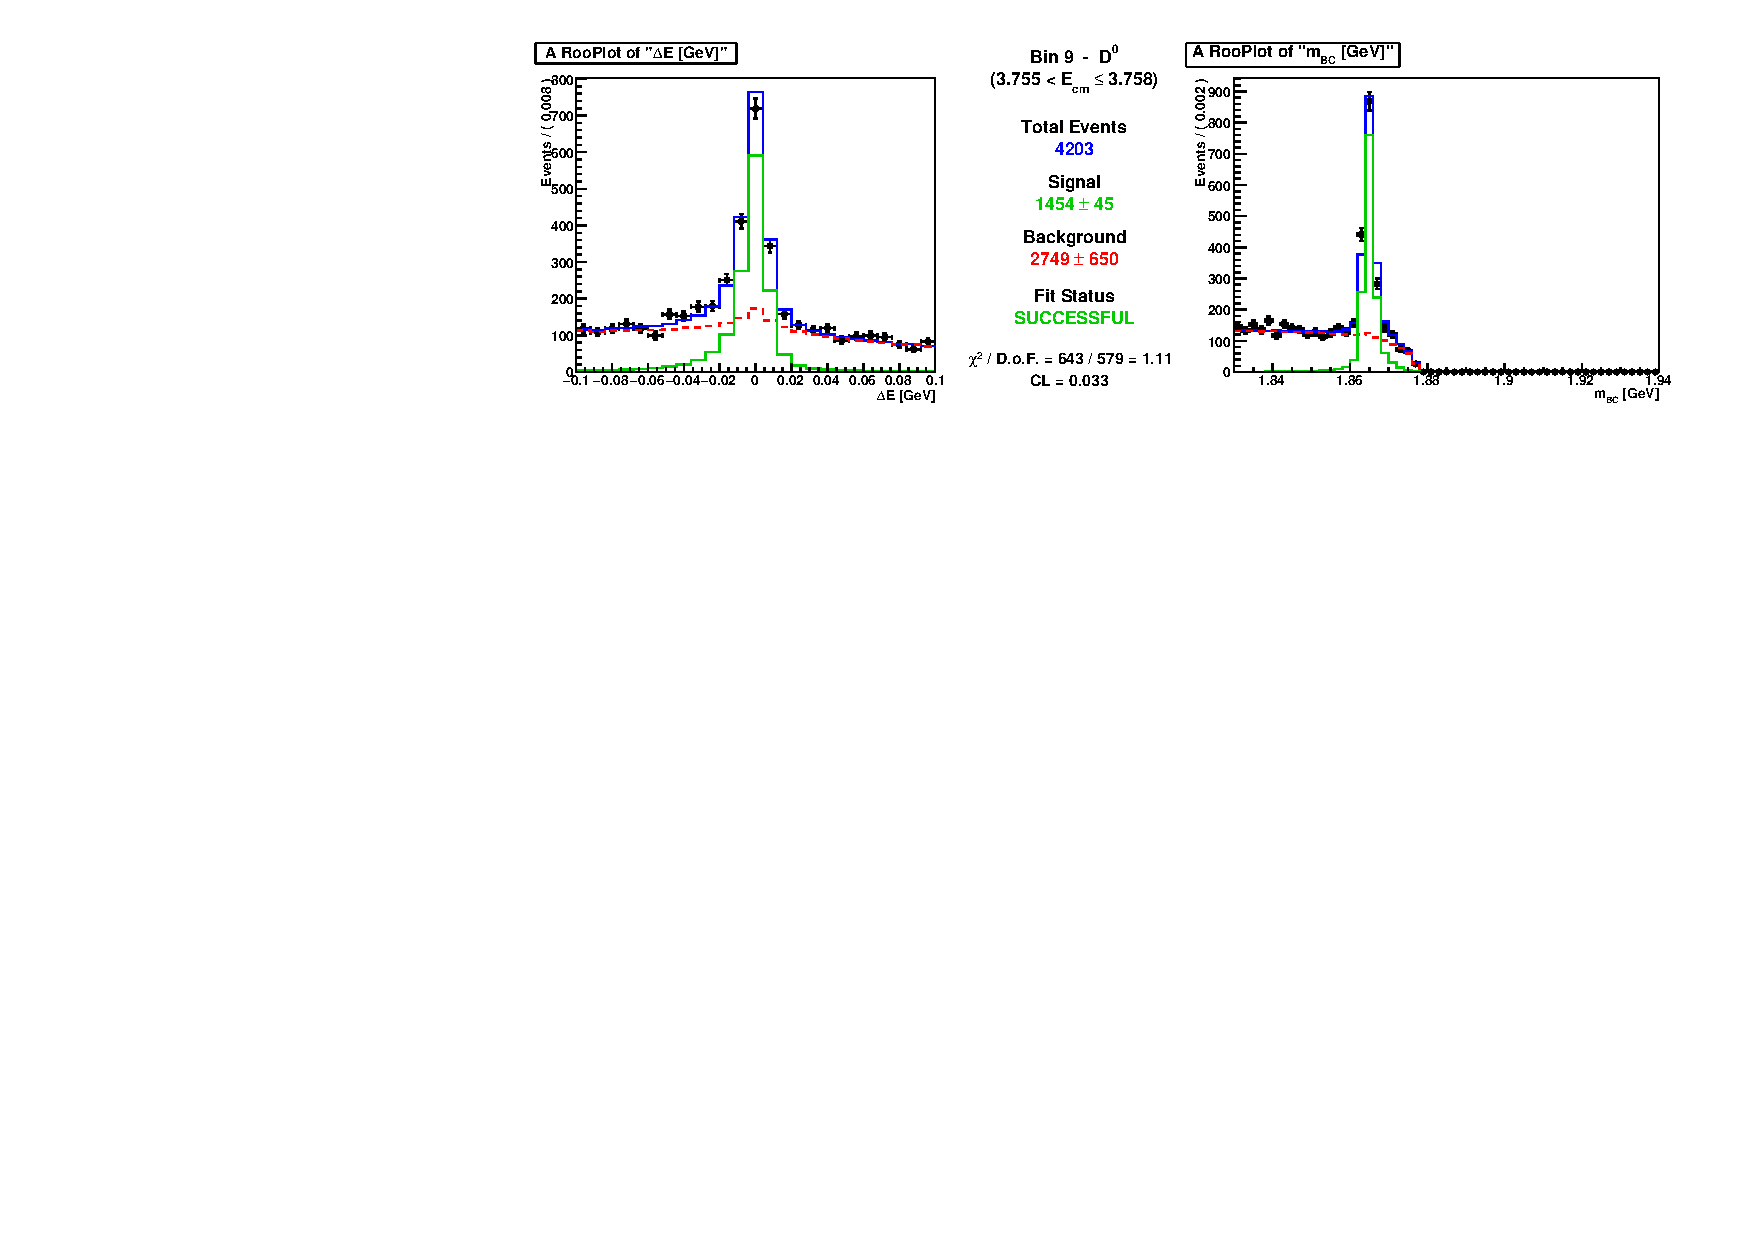
\includegraphics[width=\textwidth]{figures/plots/fit_results/D0_bin_09.pdf}
\caption*{Signal Fit - $\DO$ Bin 9}
\end{subfigure}

\caption{Signal Fitting Plots for $\DO$ Bins 6 - 9.}
\label{fig:DO_plots_6_9}

\end{figure}


\begin{figure}[h]

\begin{subfigure}[c]{0.99\textwidth}
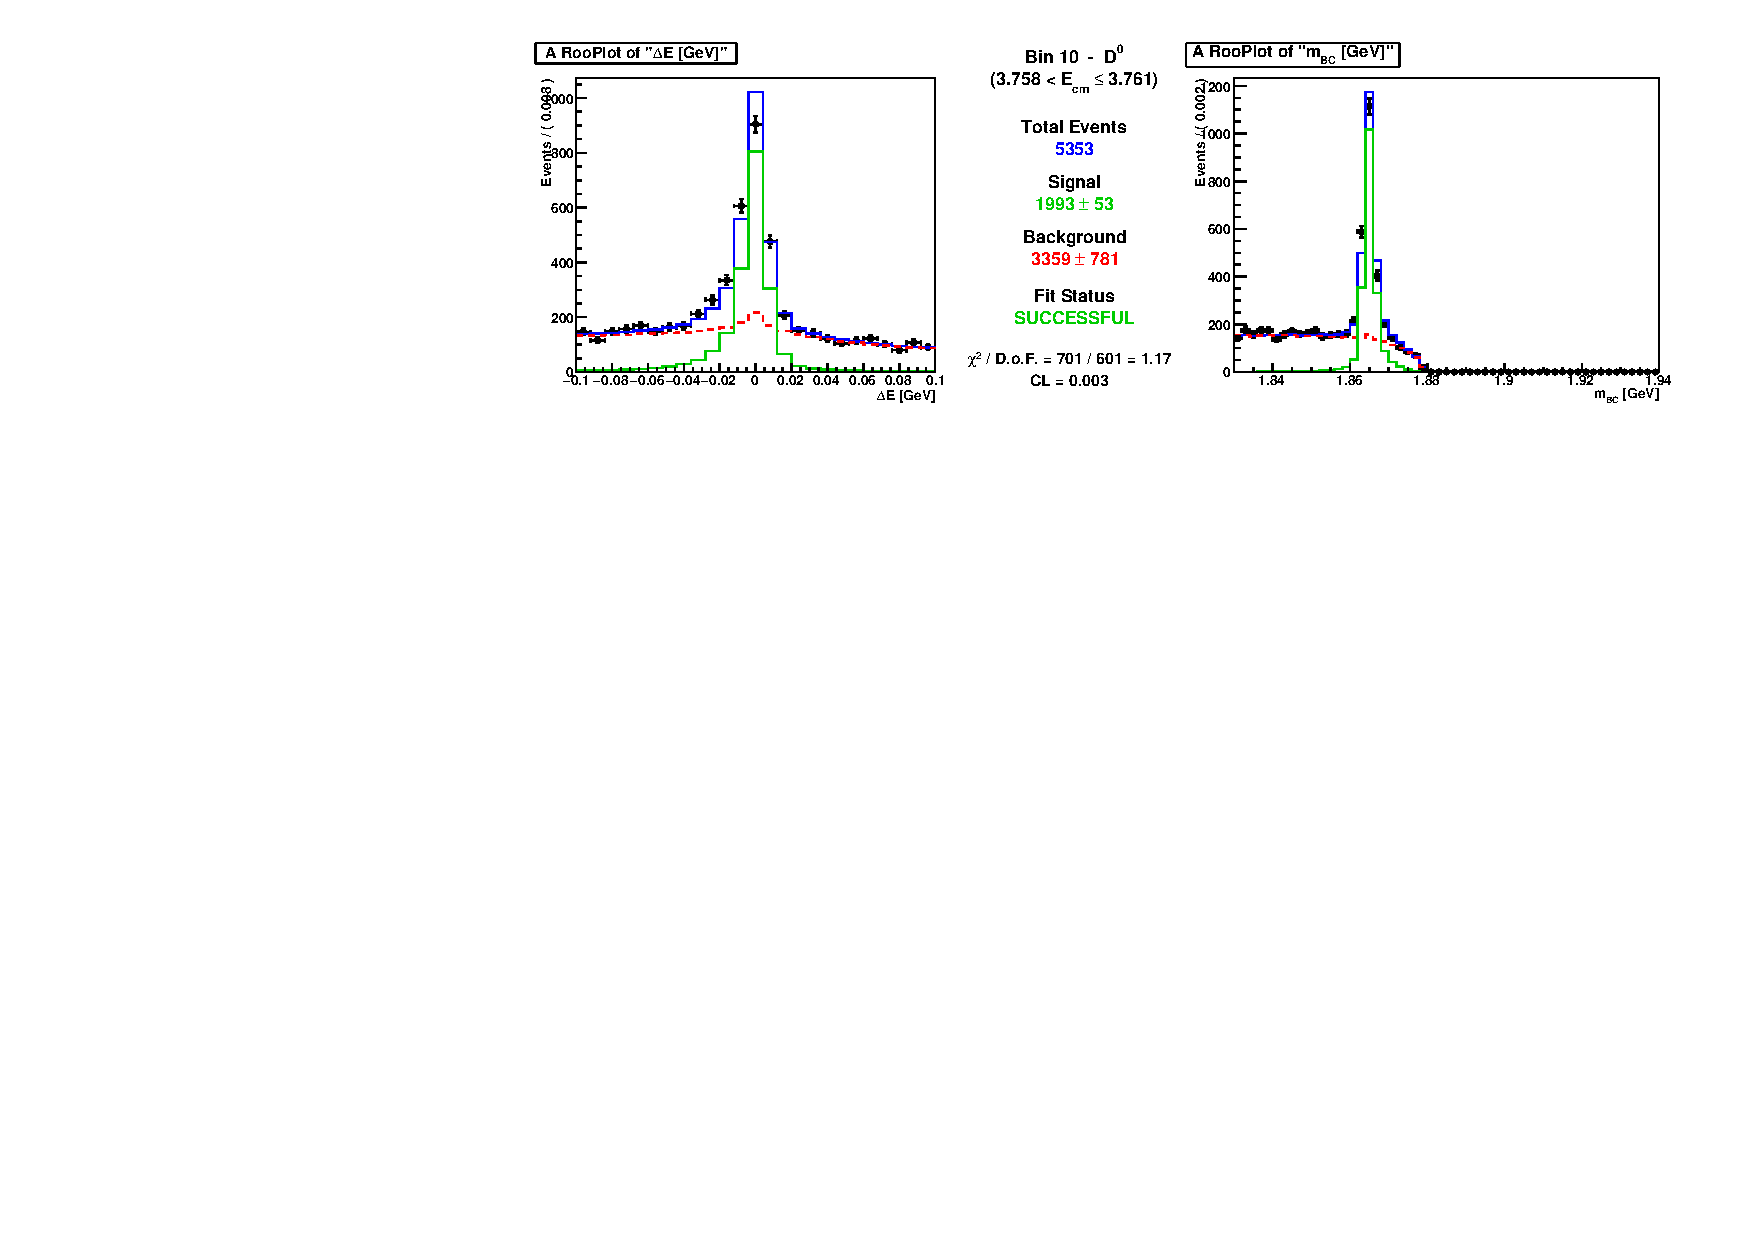
\includegraphics[width=\textwidth]{figures/plots/fit_results/D0_bin_10.pdf}
\caption*{Signal Fit - $\DO$ Bin 10}
\end{subfigure}

\vspace{5pt}

\begin{subfigure}[c]{0.99\textwidth}
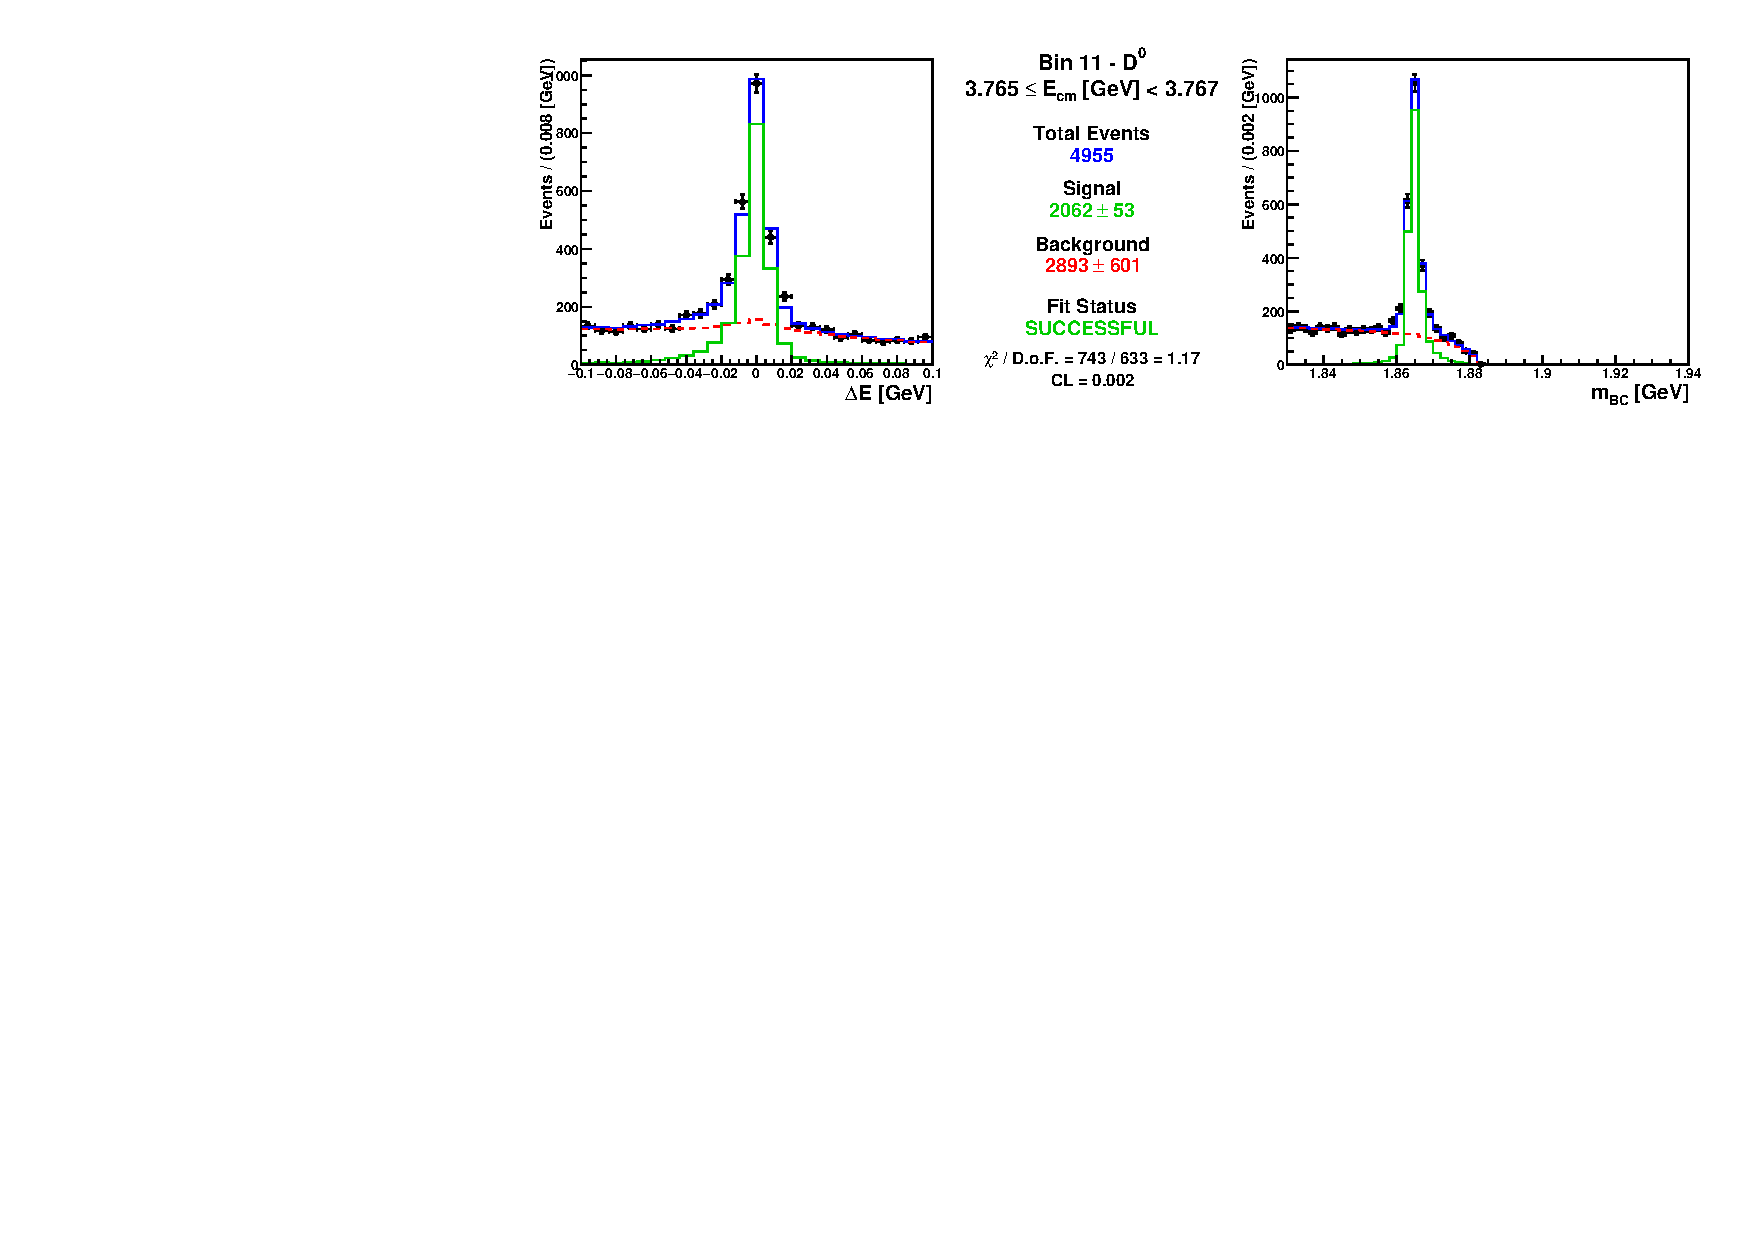
\includegraphics[width=\textwidth]{figures/plots/fit_results/D0_bin_11.pdf}
\caption*{Signal Fit - $\DO$ Bin 11}
\end{subfigure}

\vspace{5pt}

\begin{subfigure}[c]{0.99\textwidth}
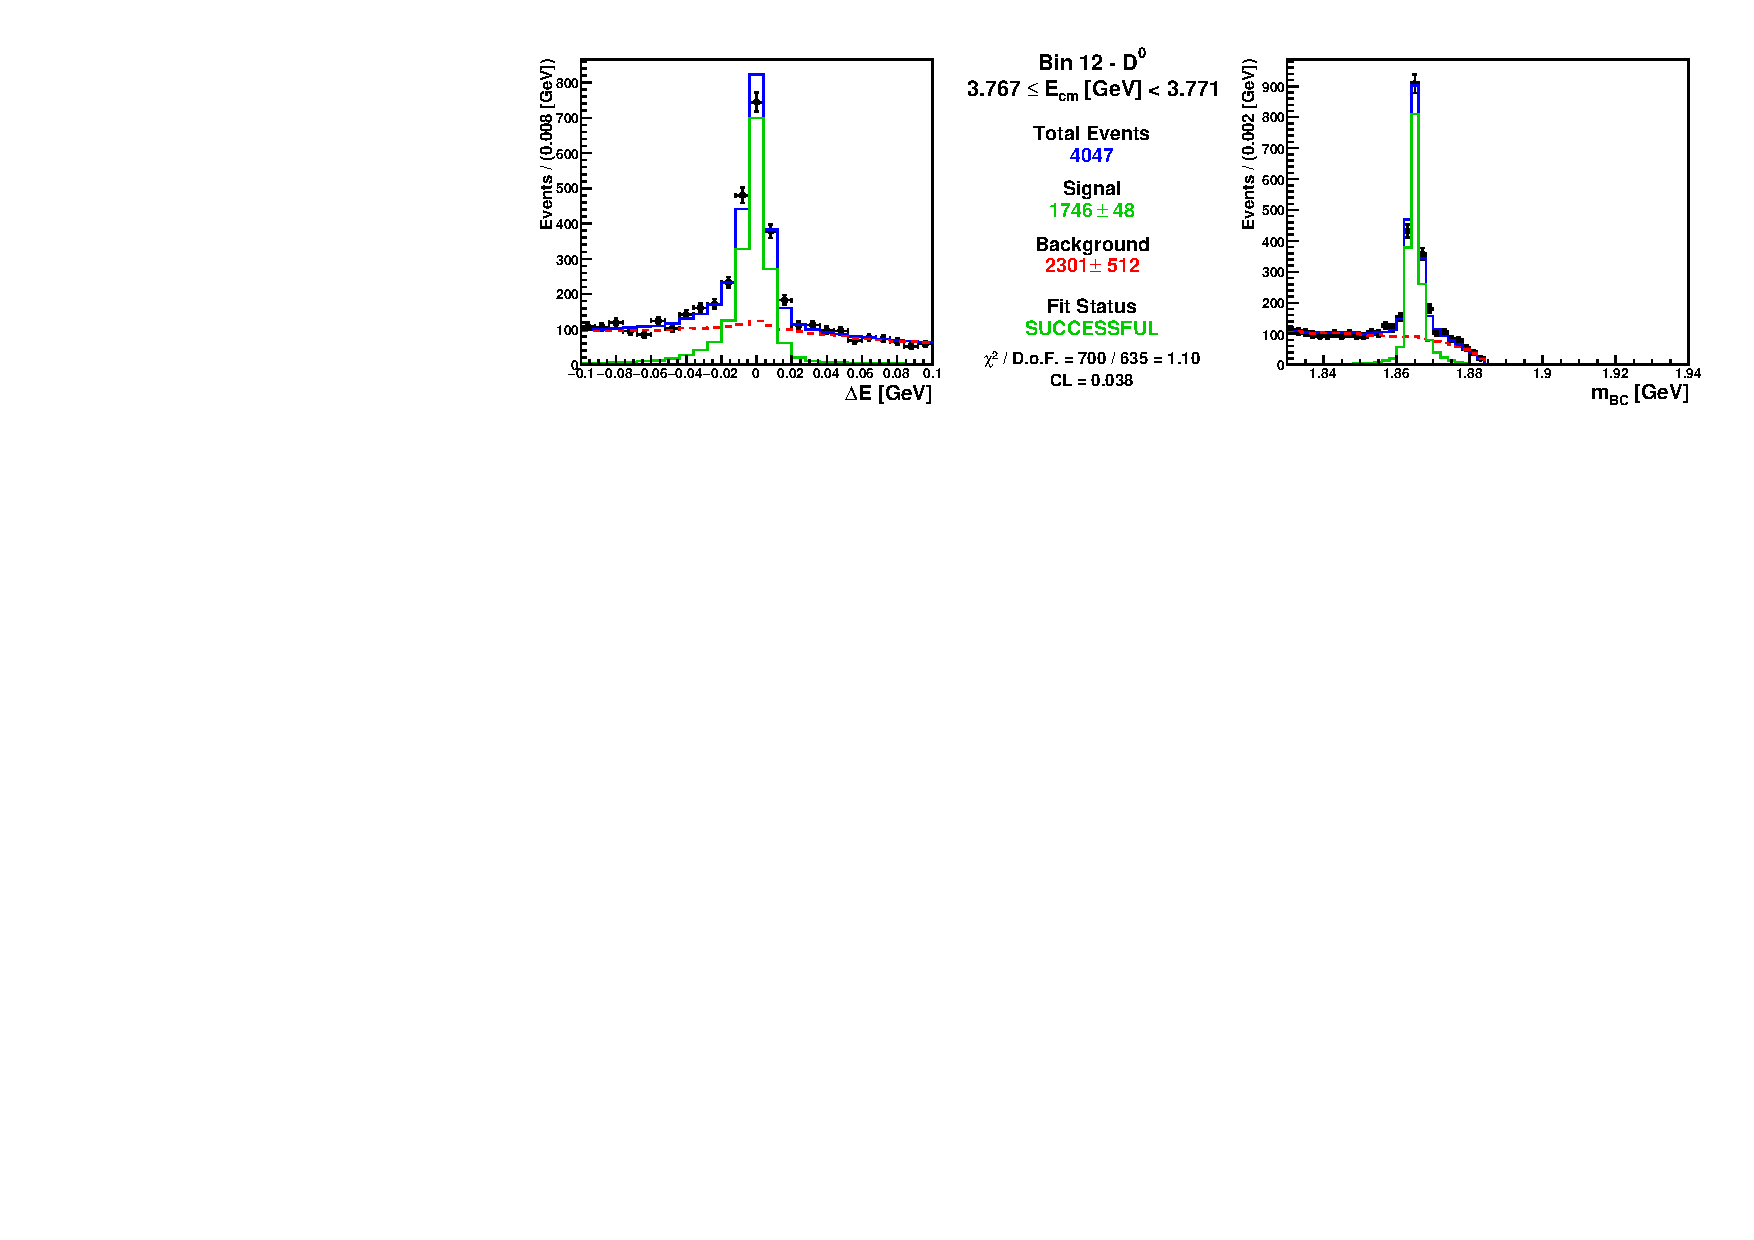
\includegraphics[width=\textwidth]{figures/plots/fit_results/D0_bin_12.pdf}
\caption*{Signal Fit - $\DO$ Bin 12}
\end{subfigure}

\vspace{5pt}

\begin{subfigure}[c]{0.99\textwidth}
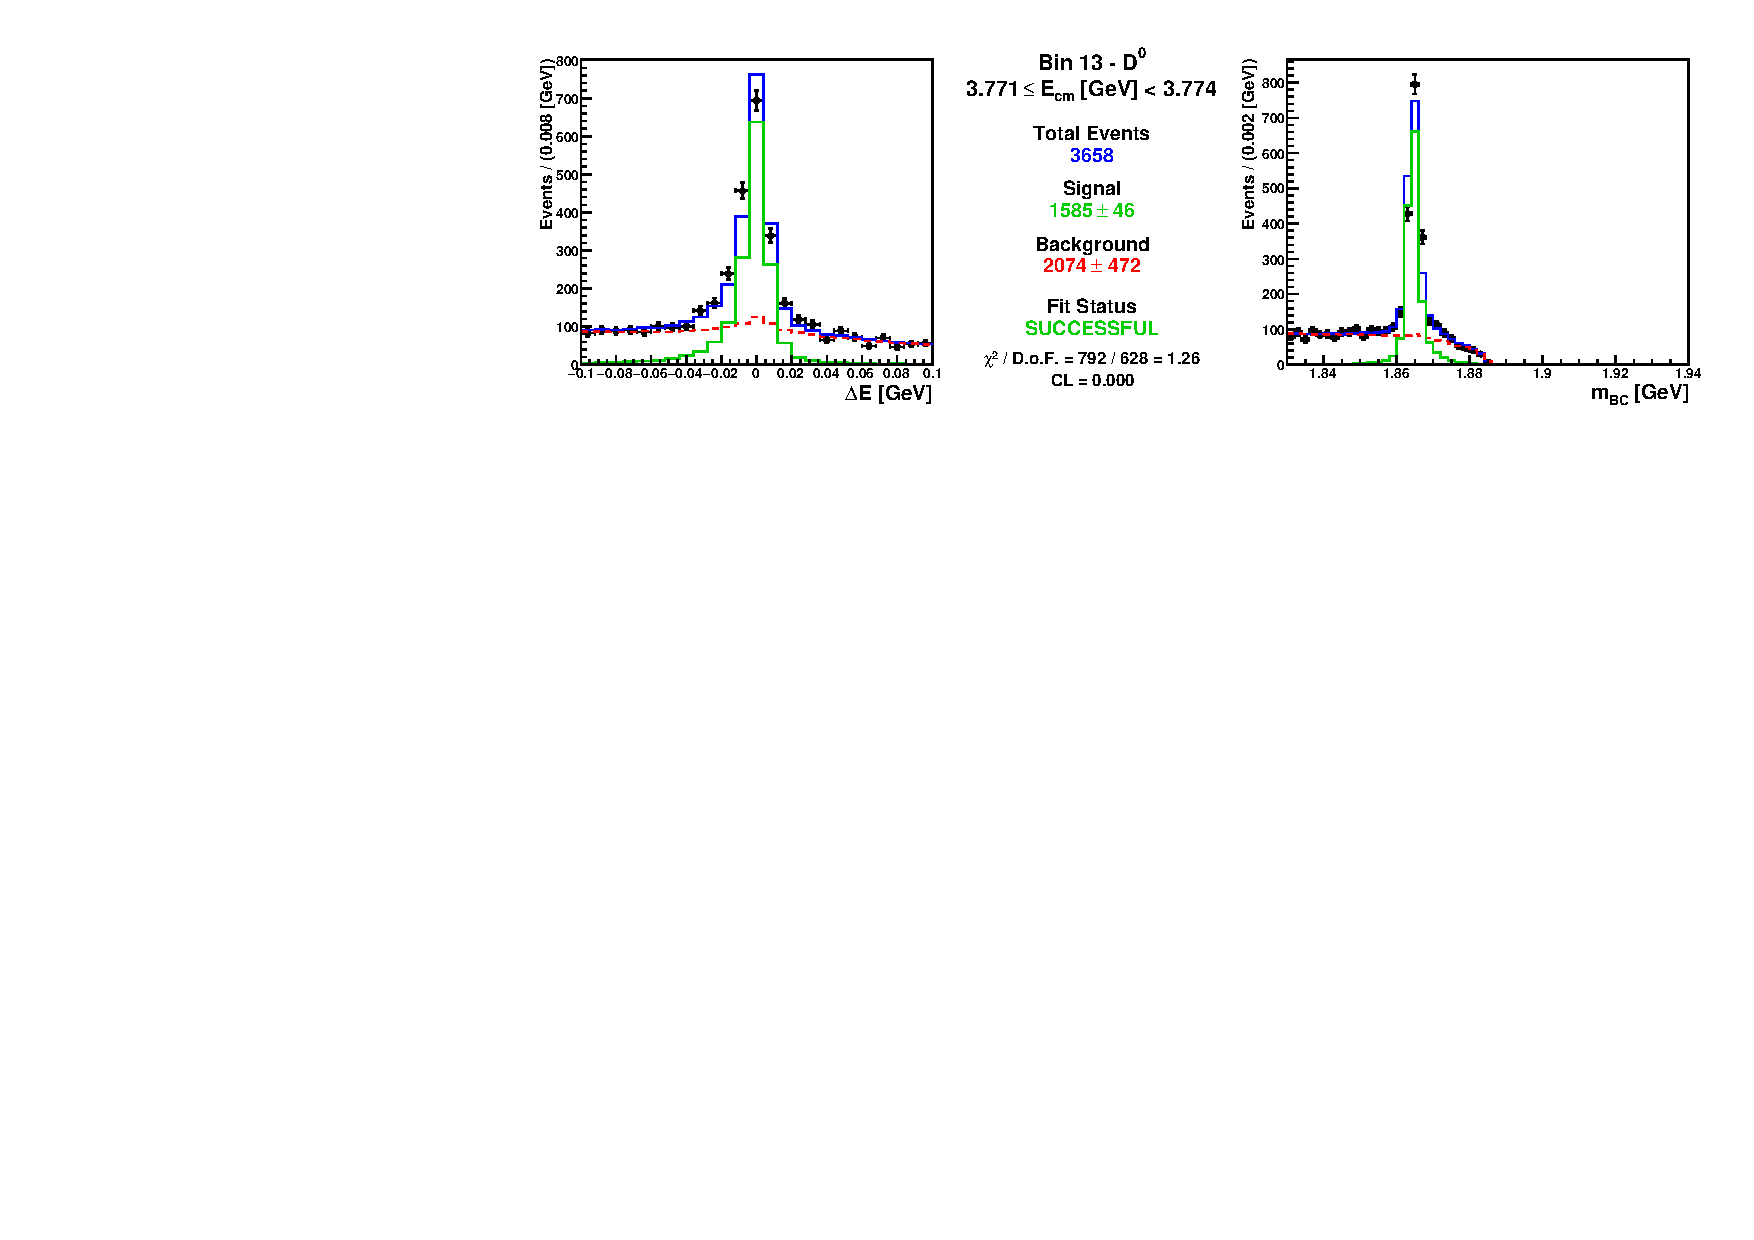
\includegraphics[width=\textwidth]{figures/plots/fit_results/D0_bin_13.pdf}
\caption*{Signal Fit - $\DO$ Bin 13}
\end{subfigure}

\caption{Signal Fitting Plots for $\DO$ Bins 10 - 13.}
\label{fig:DO_plots_10_13}

\end{figure}


\begin{figure}[h]

\begin{subfigure}[c]{0.99\textwidth}
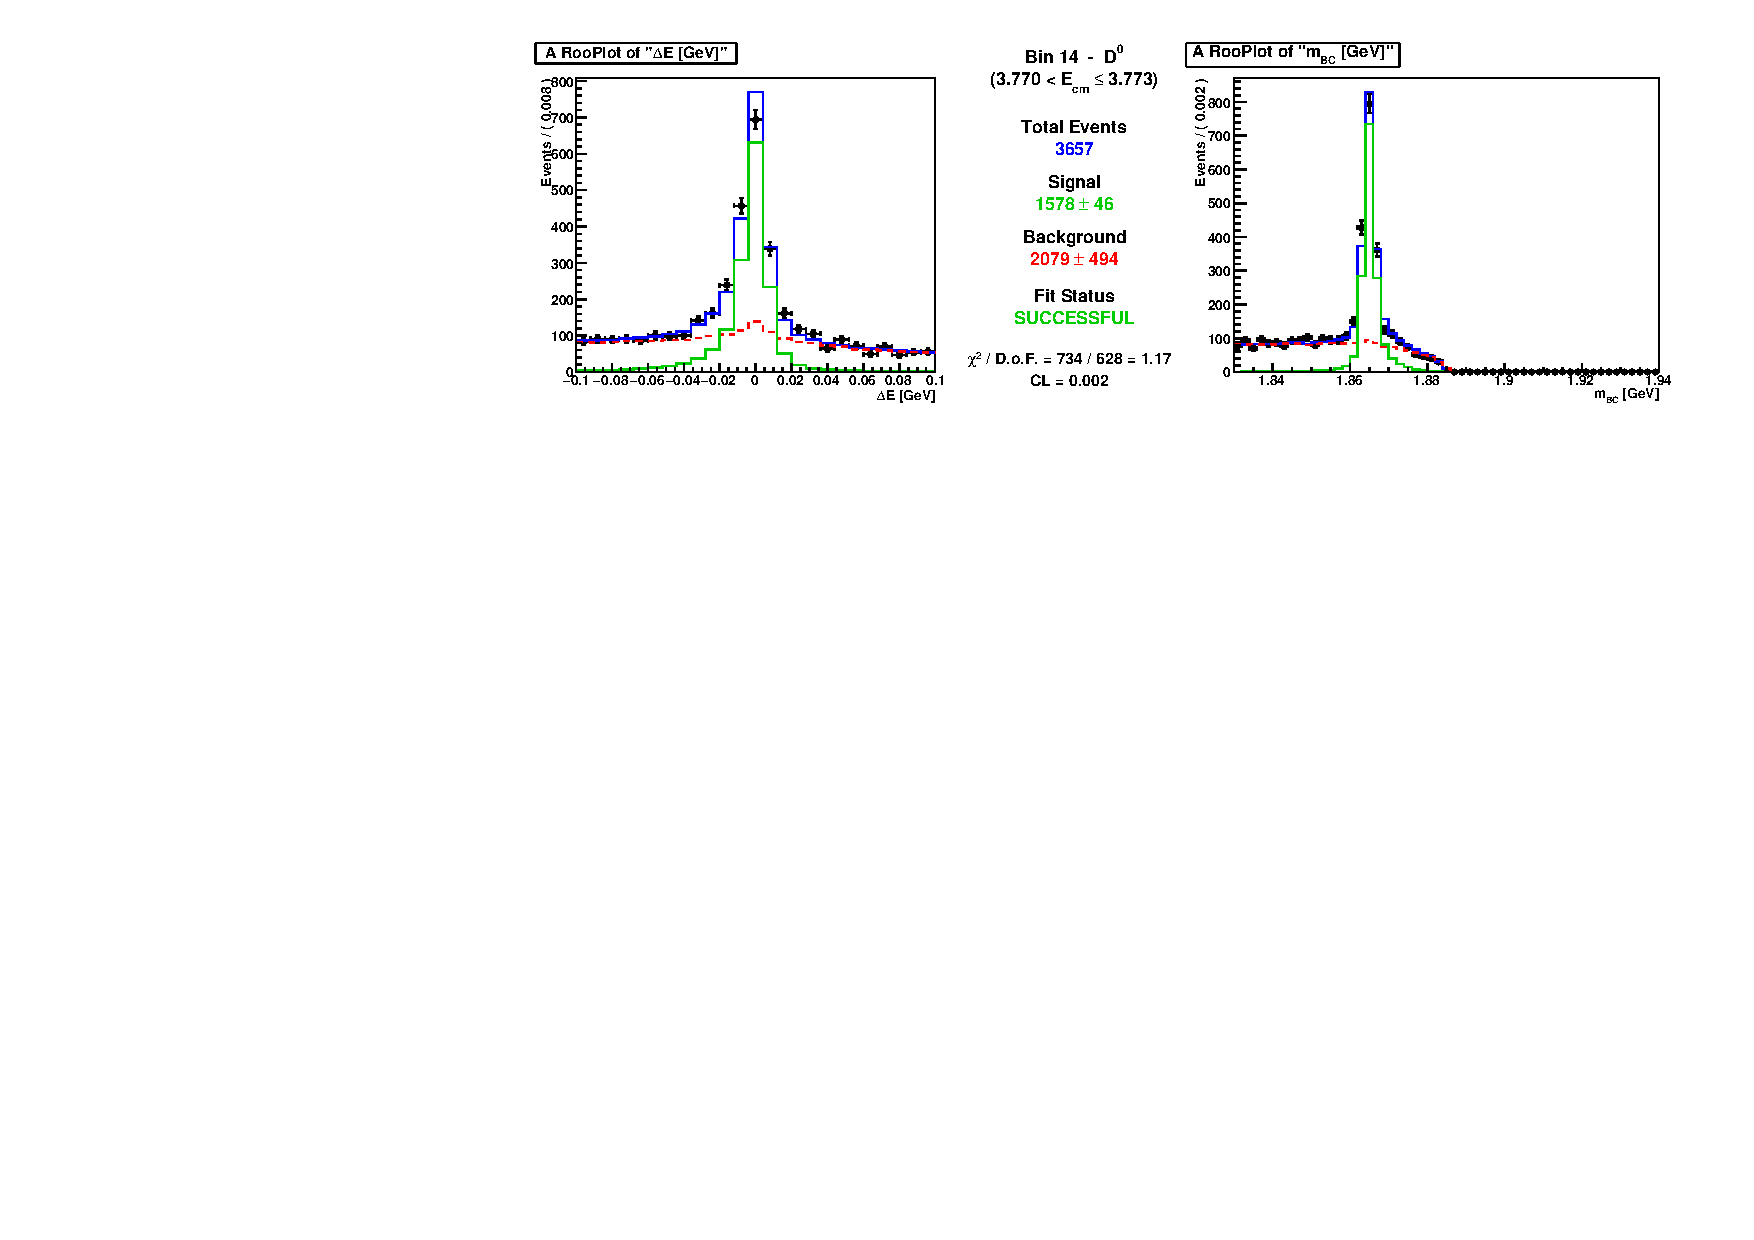
\includegraphics[width=\textwidth]{figures/plots/fit_results/D0_bin_14.pdf}
\caption*{Signal Fit - $\DO$ Bin 14}
\end{subfigure}

\vspace{5pt}

\begin{subfigure}[c]{0.99\textwidth}
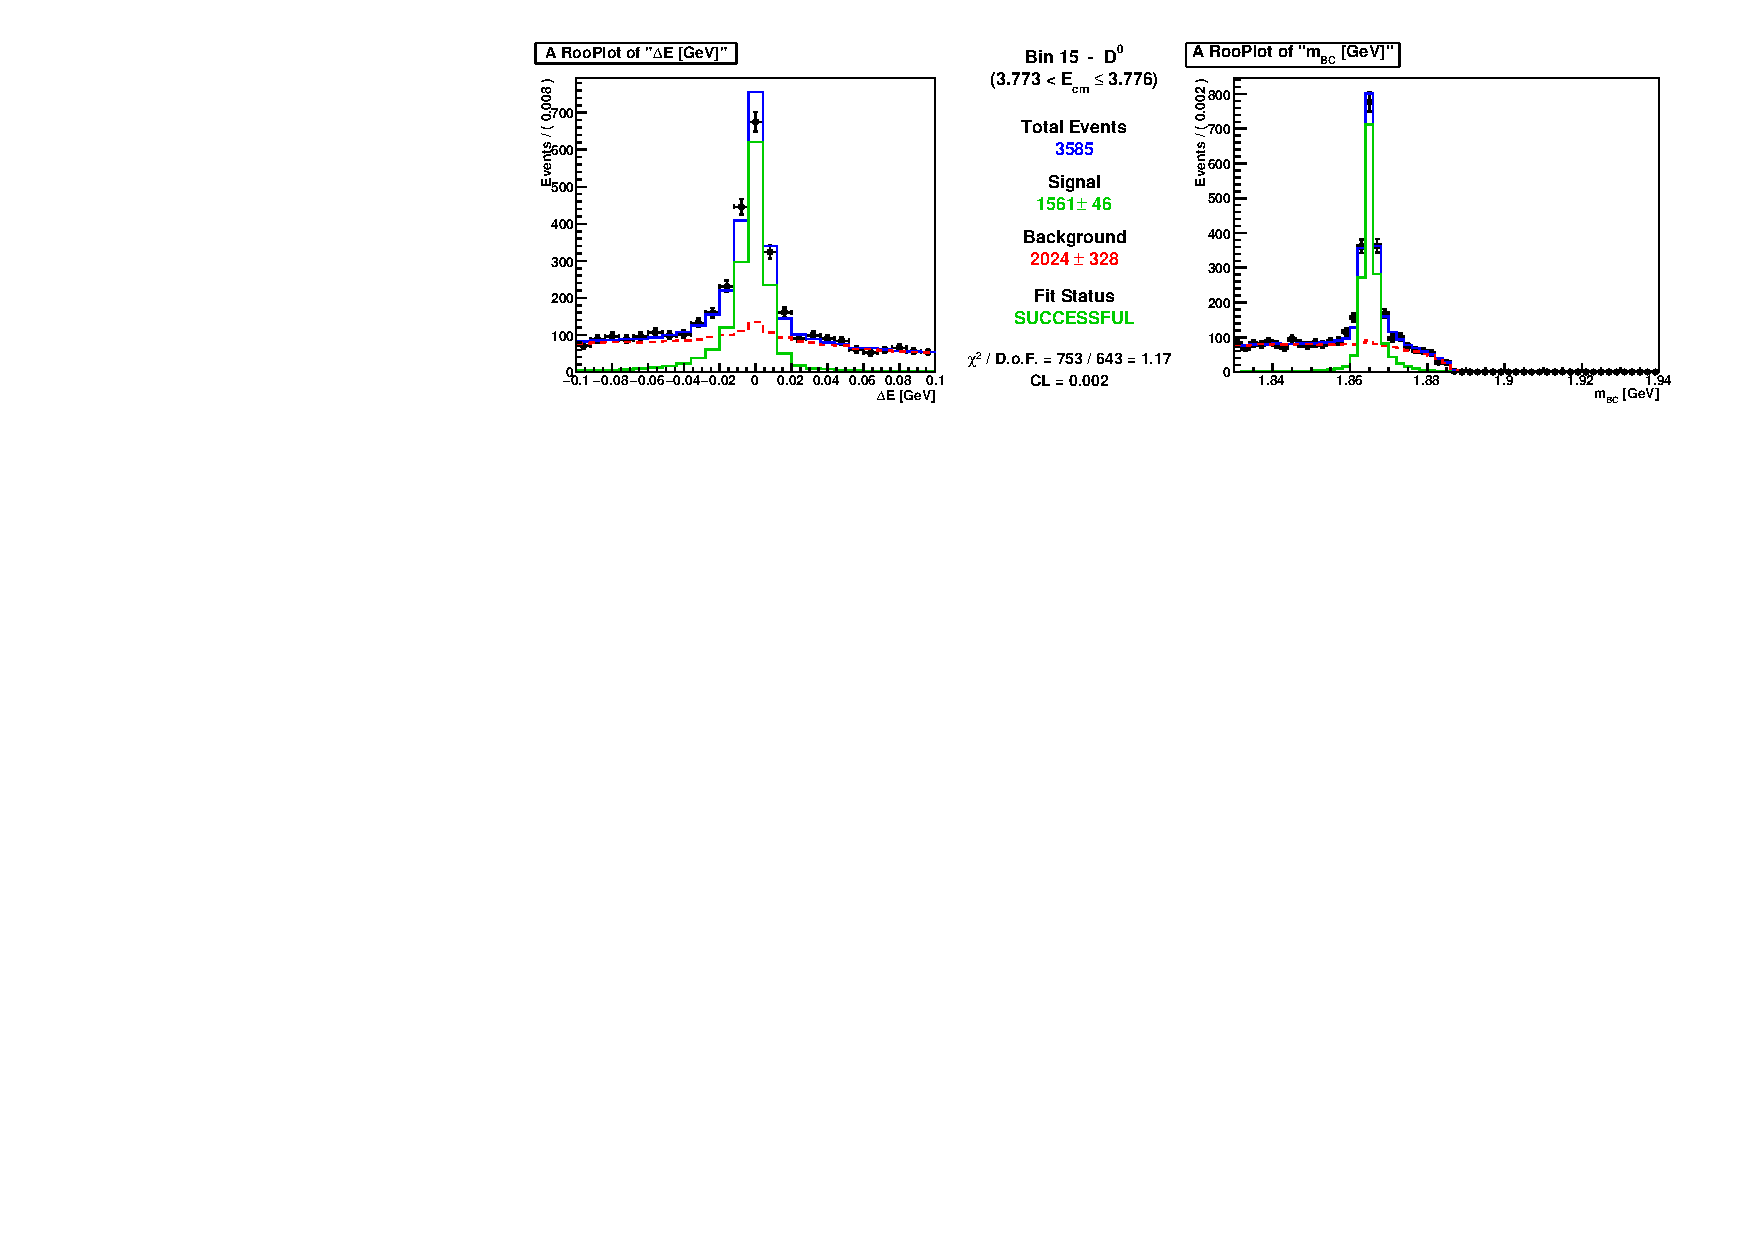
\includegraphics[width=\textwidth]{figures/plots/fit_results/D0_bin_15.pdf}
\caption*{Signal Fit - $\DO$ Bin 15}
\end{subfigure}

\vspace{5pt}

\begin{subfigure}[c]{0.99\textwidth}
\includegraphics[width=\textwidth]{figures/plots/fit_results/D0_bin_16.pdf}
\caption*{Signal Fit - $\DO$ Bin 16}
\end{subfigure}

\vspace{5pt}

\begin{subfigure}[c]{0.99\textwidth}
\includegraphics[width=\textwidth]{figures/plots/fit_results/D0_bin_17.pdf}
\caption*{Signal Fit - $\DO$ Bin 17}
\end{subfigure}

\caption{Signal Fitting Plots for $\DO$ Bins 14 - 17.}
\label{fig:DO_plots_14_17}

\end{figure}


\begin{figure}[h]

\begin{subfigure}[c]{0.99\textwidth}
\includegraphics[width=\textwidth]{figures/plots/fit_results/D0_bin_18.pdf}
\caption*{Signal Fit - $\DO$ Bin 18}
\end{subfigure}

\vspace{5pt}

\begin{subfigure}[c]{0.99\textwidth}
\includegraphics[width=\textwidth]{figures/plots/fit_results/D0_bin_19.pdf}
\caption*{Signal Fit - $\DO$ Bin 19}
\end{subfigure}

\vspace{5pt}

\begin{subfigure}[c]{0.99\textwidth}
\includegraphics[width=\textwidth]{figures/plots/fit_results/D0_bin_20.pdf}
\caption*{Signal Fit - $\DO$ Bin 20}
\end{subfigure}

\vspace{5pt}

\begin{subfigure}[c]{0.99\textwidth}
\includegraphics[width=\textwidth]{figures/plots/fit_results/D0_bin_21.pdf}
\caption*{Signal Fit - $\DO$ Bin 21}
\end{subfigure}

\caption{Signal Fitting Plots for $\DO$ Bins 18 - 21.}
\label{fig:DO_plots_18_21}

\end{figure}


\begin{figure}[h]

\begin{subfigure}[c]{0.99\textwidth}
\includegraphics[width=\textwidth]{figures/plots/fit_results/D0_bin_22.pdf}
\caption*{Signal Fit - $\DO$ Bin 22}
\end{subfigure}

\vspace{5pt}

\begin{subfigure}[c]{0.99\textwidth}
\includegraphics[width=\textwidth]{figures/plots/fit_results/D0_bin_23.pdf}
\caption*{Signal Fit - $\DO$ Bin 23}
\end{subfigure}

\vspace{5pt}

\begin{subfigure}[c]{0.99\textwidth}
\includegraphics[width=\textwidth]{figures/plots/fit_results/D0_bin_24.pdf}
\caption*{Signal Fit - $\DO$ Bin 24}
\end{subfigure}

\vspace{5pt}

\begin{subfigure}[c]{0.99\textwidth}
\includegraphics[width=\textwidth]{figures/plots/fit_results/D0_bin_25.pdf}
\caption*{Signal Fit - $\DO$ Bin 25}
\end{subfigure}

\caption{Signal Fitting Plots for $\DO$ Bins 22 - 25.}
\label{fig:DO_plots_22_25}

\end{figure}


\begin{figure}[h]

\begin{subfigure}[c]{0.99\textwidth}
\includegraphics[width=\textwidth]{figures/plots/fit_results/D0_bin_26.pdf}
\caption*{Signal Fit - $\DO$ Bin 26}
\end{subfigure}

\vspace{5pt}

\begin{subfigure}[c]{0.99\textwidth}
\includegraphics[width=\textwidth]{figures/plots/fit_results/D0_bin_27.pdf}
\caption*{Signal Fit - $\DO$ Bin 27}
\end{subfigure}

\vspace{5pt}

\begin{subfigure}[c]{0.99\textwidth}
\includegraphics[width=\textwidth]{figures/plots/fit_results/D0_bin_28.pdf}
\caption*{Signal Fit - $\DO$ Bin 28}
\end{subfigure}

\vspace{5pt}

\begin{subfigure}[c]{0.99\textwidth}
\includegraphics[width=\textwidth]{figures/plots/fit_results/D0_bin_29.pdf}
\caption*{Signal Fit - $\DO$ Bin 29}
\end{subfigure}

\caption{Signal Fitting Plots for $\DO$ Bins 26 - 29.}
\label{fig:DO_plots_26_29}

\end{figure}


\begin{figure}[h]

\begin{subfigure}[c]{0.99\textwidth}
\includegraphics[width=\textwidth]{figures/plots/fit_results/D0_bin_30.pdf}
\caption*{Signal Fit - $\DO$ Bin 30}
\end{subfigure}

\vspace{5pt}

\begin{subfigure}[c]{0.99\textwidth}
\includegraphics[width=\textwidth]{figures/plots/fit_results/D0_bin_31.pdf}
\caption*{Signal Fit - $\DO$ Bin 31}
\end{subfigure}

\vspace{5pt}

\begin{subfigure}[c]{0.99\textwidth}
\includegraphics[width=\textwidth]{figures/plots/fit_results/D0_bin_32.pdf}
\caption*{Signal Fit - $\DO$ Bin 32}
\end{subfigure}

\vspace{5pt}

\begin{subfigure}[c]{0.99\textwidth}
\includegraphics[width=\textwidth]{figures/plots/fit_results/D0_bin_33.pdf}
\caption*{Signal Fit - $\DO$ Bin 33}
\end{subfigure}

\caption{Signal Fitting Plots for $\DO$ Bins 30 - 33.}
\label{fig:DO_plots_30_33}

\end{figure}


\begin{figure}[h]

\begin{subfigure}[c]{0.99\textwidth}
\includegraphics[width=\textwidth]{figures/plots/fit_results/D0_bin_34.pdf}
\caption*{Signal Fit - $\DO$ Bin 34}
\end{subfigure}

\caption{Signal Fitting Plots for $\DO$ Bin 34.}
\label{fig:DO_plots_34}

\end{figure}


\chapter{$\Dp$ Signal Fits}
\label{app:Dp_signal_fits}

\begin{figure}[h]

\begin{subfigure}[c]{0.99\textwidth}
\includegraphics[width=\textwidth]{figures/plots/fit_results/Dp_bin_03.pdf}
\caption*{Signal Fit - $\Dp$ Bin 3}
\end{subfigure}

\vspace{5pt}

\begin{subfigure}[c]{0.99\textwidth}
\includegraphics[width=\textwidth]{figures/plots/fit_results/Dp_bin_04.pdf}
\caption*{Signal Fit - $\Dp$ Bin 4}
\end{subfigure}

\caption{Signal Fitting Plots for $\Dp$ Bins 3 - 4.}
\label{fig:Dp_plots_3_4}

\end{figure}


\begin{figure}[h]

\begin{subfigure}[c]{0.99\textwidth}
\includegraphics[width=\textwidth]{figures/plots/fit_results/Dp_bin_05.pdf}
\caption*{Signal Fit - $\Dp$ Bin 5}
\end{subfigure}

\vspace{5pt}

\begin{subfigure}[c]{0.99\textwidth}
\includegraphics[width=\textwidth]{figures/plots/fit_results/Dp_bin_06.pdf}
\caption*{Signal Fit - $\Dp$ Bin 6}
\end{subfigure}

\vspace{5pt}

\begin{subfigure}[c]{0.99\textwidth}
\includegraphics[width=\textwidth]{figures/plots/fit_results/Dp_bin_07.pdf}
\caption*{Signal Fit - $\Dp$ Bin 7}
\end{subfigure}

\vspace{5pt}

\begin{subfigure}[c]{0.99\textwidth}
\includegraphics[width=\textwidth]{figures/plots/fit_results/Dp_bin_08.pdf}
\caption*{Signal Fit - $\Dp$ Bin 8}
\end{subfigure}

\caption{Signal Fitting Plots for $\Dp$ Bins 5 - 8.}
\label{fig:Dp_plots_5_8}

\end{figure}


\begin{figure}[h]

\begin{subfigure}[c]{0.99\textwidth}
\includegraphics[width=\textwidth]{figures/plots/fit_results/Dp_bin_09.pdf}
\caption*{Signal Fit - $\Dp$ Bin 9}
\end{subfigure}

\vspace{5pt}

\begin{subfigure}[c]{0.99\textwidth}
\includegraphics[width=\textwidth]{figures/plots/fit_results/Dp_bin_10.pdf}
\caption*{Signal Fit - $\Dp$ Bin 10}
\end{subfigure}

\vspace{5pt}

\begin{subfigure}[c]{0.99\textwidth}
\includegraphics[width=\textwidth]{figures/plots/fit_results/Dp_bin_11.pdf}
\caption*{Signal Fit - $\Dp$ Bin 11}
\end{subfigure}

\vspace{5pt}

\begin{subfigure}[c]{0.99\textwidth}
\includegraphics[width=\textwidth]{figures/plots/fit_results/Dp_bin_12.pdf}
\caption*{Signal Fit - $\Dp$ Bin 12}
\end{subfigure}

\caption{Signal Fitting Plots for $\Dp$ Bins 6 - 12.}
\label{fig:Dp_plots_6_12}

\end{figure}


\begin{figure}[h]

\begin{subfigure}[c]{0.99\textwidth}
\includegraphics[width=\textwidth]{figures/plots/fit_results/Dp_bin_13.pdf}
\caption*{Signal Fit - $\Dp$ Bin 13}
\end{subfigure}

\vspace{5pt}

\begin{subfigure}[c]{0.99\textwidth}
\includegraphics[width=\textwidth]{figures/plots/fit_results/Dp_bin_14.pdf}
\caption*{Signal Fit - $\Dp$ Bin 14}
\end{subfigure}

\vspace{5pt}

\begin{subfigure}[c]{0.99\textwidth}
\includegraphics[width=\textwidth]{figures/plots/fit_results/Dp_bin_15.pdf}
\caption*{Signal Fit - $\Dp$ Bin 15}
\end{subfigure}

\vspace{5pt}

\begin{subfigure}[c]{0.99\textwidth}
\includegraphics[width=\textwidth]{figures/plots/fit_results/Dp_bin_16.pdf}
\caption*{Signal Fit - $\Dp$ Bin 16}
\end{subfigure}

\caption{Signal Fitting Plots for $\Dp$ Bins 13 - 16.}
\label{fig:Dp_plots_13_16}

\end{figure}


\begin{figure}[h]

\begin{subfigure}[c]{0.99\textwidth}
\includegraphics[width=\textwidth]{figures/plots/fit_results/Dp_bin_17.pdf}
\caption*{Signal Fit - $\Dp$ Bin 17}
\end{subfigure}

\vspace{5pt}

\begin{subfigure}[c]{0.99\textwidth}
\includegraphics[width=\textwidth]{figures/plots/fit_results/Dp_bin_18.pdf}
\caption*{Signal Fit - $\Dp$ Bin 18}
\end{subfigure}

\vspace{5pt}

\begin{subfigure}[c]{0.99\textwidth}
\includegraphics[width=\textwidth]{figures/plots/fit_results/Dp_bin_19.pdf}
\caption*{Signal Fit - $\Dp$ Bin 19}
\end{subfigure}

\vspace{5pt}

\begin{subfigure}[c]{0.99\textwidth}
\includegraphics[width=\textwidth]{figures/plots/fit_results/Dp_bin_20.pdf}
\caption*{Signal Fit - $\Dp$ Bin 20}
\end{subfigure}

\caption{Signal Fitting Plots for $\Dp$ Bins 17 - 20.}
\label{fig:Dp_plots_17_20}

\end{figure}


\begin{figure}[h]

\begin{subfigure}[c]{0.99\textwidth}
\includegraphics[width=\textwidth]{figures/plots/fit_results/Dp_bin_21.pdf}
\caption*{Signal Fit - $\Dp$ Bin 21}
\end{subfigure}

\vspace{5pt}

\begin{subfigure}[c]{0.99\textwidth}
\includegraphics[width=\textwidth]{figures/plots/fit_results/Dp_bin_22.pdf}
\caption*{Signal Fit - $\Dp$ Bin 22}
\end{subfigure}

\vspace{5pt}

\begin{subfigure}[c]{0.99\textwidth}
\includegraphics[width=\textwidth]{figures/plots/fit_results/Dp_bin_23.pdf}
\caption*{Signal Fit - $\Dp$ Bin 23}
\end{subfigure}

\vspace{5pt}

\begin{subfigure}[c]{0.99\textwidth}
\includegraphics[width=\textwidth]{figures/plots/fit_results/Dp_bin_24.pdf}
\caption*{Signal Fit - $\Dp$ Bin 24}
\end{subfigure}

\caption{Signal Fitting Plots for $\Dp$ Bins 21 - 24.}
\label{fig:Dp_plots_21_24}

\end{figure}


\begin{figure}[h]

\begin{subfigure}[c]{0.99\textwidth}
\includegraphics[width=\textwidth]{figures/plots/fit_results/Dp_bin_25.pdf}
\caption*{Signal Fit - $\Dp$ Bin 25}
\end{subfigure}

\vspace{5pt}

\begin{subfigure}[c]{0.99\textwidth}
\includegraphics[width=\textwidth]{figures/plots/fit_results/Dp_bin_26.pdf}
\caption*{Signal Fit - $\Dp$ Bin 26}
\end{subfigure}

\vspace{5pt}

\begin{subfigure}[c]{0.99\textwidth}
\includegraphics[width=\textwidth]{figures/plots/fit_results/Dp_bin_27.pdf}
\caption*{Signal Fit - $\Dp$ Bin 27}
\end{subfigure}

\vspace{5pt}

\begin{subfigure}[c]{0.99\textwidth}
\includegraphics[width=\textwidth]{figures/plots/fit_results/Dp_bin_28.pdf}
\caption*{Signal Fit - $\Dp$ Bin 28}
\end{subfigure}

\caption{Signal Fitting Plots for $\Dp$ Bins 25 - 28.}
\label{fig:Dp_plots_25_28}

\end{figure}


\begin{figure}[h]

\begin{subfigure}[c]{0.99\textwidth}
\includegraphics[width=\textwidth]{figures/plots/fit_results/Dp_bin_29.pdf}
\caption*{Signal Fit - $\Dp$ Bin 29}
\end{subfigure}

\vspace{5pt}

\begin{subfigure}[c]{0.99\textwidth}
\includegraphics[width=\textwidth]{figures/plots/fit_results/Dp_bin_30.pdf}
\caption*{Signal Fit - $\Dp$ Bin 30}
\end{subfigure}

\vspace{5pt}

\begin{subfigure}[c]{0.99\textwidth}
\includegraphics[width=\textwidth]{figures/plots/fit_results/Dp_bin_31.pdf}
\caption*{Signal Fit - $\Dp$ Bin 31}
\end{subfigure}

\vspace{5pt}

\begin{subfigure}[c]{0.99\textwidth}
\includegraphics[width=\textwidth]{figures/plots/fit_results/Dp_bin_32.pdf}
\caption*{Signal Fit - $\Dp$ Bin 32}
\end{subfigure}

\caption{Signal Fitting Plots for $\Dp$ Bins 29 - 32.}
\label{fig:Dp_plots_29_32}

\end{figure}


\begin{figure}[h]

\begin{subfigure}[c]{0.99\textwidth}
\includegraphics[width=\textwidth]{figures/plots/fit_results/Dp_bin_33.pdf}
\caption*{Signal Fit - $\Dp$ Bin 33}
\end{subfigure}

\vspace{5pt}

\begin{subfigure}[c]{0.99\textwidth}
\includegraphics[width=\textwidth]{figures/plots/fit_results/Dp_bin_34.pdf}
\caption*{Signal Fit - $\Dp$ Bin 34}
\end{subfigure}

\caption{Signal Fitting Plots for $\Dp$ Bins 33 - 34.}
\label{fig:Dp_plots_33_34}

\end{figure}


\chapter{Scan Data Hadronic Counting Fits}
\label{app:nonDDbar_hadron_counts_scan}

\begin{figure}[H]
\centering
\includegraphics[scale=0.25]{figures/plots/nonDDbar_fit_results/scan/fit_scan_00_data_SHAD.pdf}
\hspace{-0.5cm}
\includegraphics[scale=0.25]{figures/plots/nonDDbar_fit_results/scan/fit_scan_00_data_LHAD.pdf}
\hspace{-0.5cm}
\includegraphics[scale=0.25]{figures/plots/nonDDbar_fit_results/scan/fit_scan_00_data_THAD.pdf}
\caption{The number of hadrons found in the 3734 (Scan) data sample.}
{This includes results for SHAD (left), LHAD (middle), and THAD (right).}
\label{fig:hadron_fits_scan_00}
\end{figure}

\begin{figure}[H]
\centering
\includegraphics[scale=0.25]{figures/plots/nonDDbar_fit_results/scan/fit_scan_01_data_SHAD.pdf}
\hspace{-0.5cm}
\includegraphics[scale=0.25]{figures/plots/nonDDbar_fit_results/scan/fit_scan_01_data_LHAD.pdf}
\hspace{-0.5cm}
\includegraphics[scale=0.25]{figures/plots/nonDDbar_fit_results/scan/fit_scan_01_data_THAD.pdf}
\caption{The number of hadrons found in the 3736 (Scan) data sample.}
{This includes results for SHAD (left), LHAD (middle), and THAD (right).}
\label{fig:hadron_fits_scan_01}
\end{figure}

\begin{figure}[H]
\centering
\includegraphics[scale=0.25]{figures/plots/nonDDbar_fit_results/scan/fit_scan_02_data_SHAD.pdf}
\hspace{-0.5cm}
\includegraphics[scale=0.25]{figures/plots/nonDDbar_fit_results/scan/fit_scan_02_data_LHAD.pdf}
\hspace{-0.5cm}
\includegraphics[scale=0.25]{figures/plots/nonDDbar_fit_results/scan/fit_scan_02_data_THAD.pdf}
\caption{The number of hadrons found in the 3744 (Scan) data sample.}
{This includes results for SHAD (left), LHAD (middle), and THAD (right).}
\label{fig:hadron_fits_scan_02}
\end{figure}

\begin{figure}[H]
\centering
\includegraphics[scale=0.25]{figures/plots/nonDDbar_fit_results/scan/fit_scan_03_data_SHAD.pdf}
\hspace{-0.5cm}
\includegraphics[scale=0.25]{figures/plots/nonDDbar_fit_results/scan/fit_scan_03_data_LHAD.pdf}
\hspace{-0.5cm}
\includegraphics[scale=0.25]{figures/plots/nonDDbar_fit_results/scan/fit_scan_03_data_THAD.pdf}
\caption{The number of hadrons found in the 3748 (Scan) data sample.}
{This includes results for SHAD (left), LHAD (middle), and THAD (right).}
\label{fig:hadron_fits_scan_03}
\end{figure}

\begin{figure}[H]
\centering
\includegraphics[scale=0.25]{figures/plots/nonDDbar_fit_results/scan/fit_scan_04_data_SHAD.pdf}
\hspace{-0.5cm}
\includegraphics[scale=0.25]{figures/plots/nonDDbar_fit_results/scan/fit_scan_04_data_LHAD.pdf}
\hspace{-0.5cm}
\includegraphics[scale=0.25]{figures/plots/nonDDbar_fit_results/scan/fit_scan_04_data_THAD.pdf}
\caption{The number of hadrons found in the 3750 (Scan) data sample.}
{This includes results for SHAD (left), LHAD (middle), and THAD (right).}
\label{fig:hadron_fits_scan_04}
\end{figure}

\begin{figure}[H]
\centering
\includegraphics[scale=0.25]{figures/plots/nonDDbar_fit_results/scan/fit_scan_05_data_SHAD.pdf}
\hspace{-0.5cm}
\includegraphics[scale=0.25]{figures/plots/nonDDbar_fit_results/scan/fit_scan_05_data_LHAD.pdf}
\hspace{-0.5cm}
\includegraphics[scale=0.25]{figures/plots/nonDDbar_fit_results/scan/fit_scan_05_data_THAD.pdf}
\caption{The number of hadrons found in the 3751 (Scan) data sample.}
{This includes results for SHAD (left), LHAD (middle), and THAD (right).}
\label{fig:hadron_fits_scan_05}
\end{figure}

\begin{figure}[H]
\centering
\includegraphics[scale=0.25]{figures/plots/nonDDbar_fit_results/scan/fit_scan_06_data_SHAD.pdf}
\hspace{-0.5cm}
\includegraphics[scale=0.25]{figures/plots/nonDDbar_fit_results/scan/fit_scan_06_data_LHAD.pdf}
\hspace{-0.5cm}
\includegraphics[scale=0.25]{figures/plots/nonDDbar_fit_results/scan/fit_scan_06_data_THAD.pdf}
\caption{The number of hadrons found in the 3753 (Scan) data sample.}
{This includes results for SHAD (left), LHAD (middle), and THAD (right).}
\label{fig:hadron_fits_scan_06}
\end{figure}

\begin{figure}[H]
\centering
\includegraphics[scale=0.25]{figures/plots/nonDDbar_fit_results/scan/fit_scan_07_data_SHAD.pdf}
\hspace{-0.5cm}
\includegraphics[scale=0.25]{figures/plots/nonDDbar_fit_results/scan/fit_scan_07_data_LHAD.pdf}
\hspace{-0.5cm}
\includegraphics[scale=0.25]{figures/plots/nonDDbar_fit_results/scan/fit_scan_07_data_THAD.pdf}
\caption{The number of hadrons found in the 3755 (Scan) data sample.}
{This includes results for SHAD (left), LHAD (middle), and THAD (right).}
\label{fig:hadron_fits_scan_07}
\end{figure}

\begin{figure}[H]
\centering
\includegraphics[scale=0.25]{figures/plots/nonDDbar_fit_results/scan/fit_scan_08_data_SHAD.pdf}
\hspace{-0.5cm}
\includegraphics[scale=0.25]{figures/plots/nonDDbar_fit_results/scan/fit_scan_08_data_LHAD.pdf}
\hspace{-0.5cm}
\includegraphics[scale=0.25]{figures/plots/nonDDbar_fit_results/scan/fit_scan_08_data_THAD.pdf}
\caption{The number of hadrons found in the 3756 (Scan) data sample.}
{This includes results for SHAD (left), LHAD (middle), and THAD (right).}
\label{fig:hadron_fits_scan_08}
\end{figure}

\begin{figure}[H]
\centering
\includegraphics[scale=0.25]{figures/plots/nonDDbar_fit_results/scan/fit_scan_09_data_SHAD.pdf}
\hspace{-0.5cm}
\includegraphics[scale=0.25]{figures/plots/nonDDbar_fit_results/scan/fit_scan_09_data_LHAD.pdf}
\hspace{-0.5cm}
\includegraphics[scale=0.25]{figures/plots/nonDDbar_fit_results/scan/fit_scan_09_data_THAD.pdf}
\caption{The number of hadrons found in the 3759 (Scan) data sample.}
{This includes results for SHAD (left), LHAD (middle), and THAD (right).}
\label{fig:hadron_fits_scan_09}
\end{figure}

\begin{figure}[H]
\centering
\includegraphics[scale=0.25]{figures/plots/nonDDbar_fit_results/scan/fit_scan_10_data_SHAD.pdf}
\hspace{-0.5cm}
\includegraphics[scale=0.25]{figures/plots/nonDDbar_fit_results/scan/fit_scan_10_data_LHAD.pdf}
\hspace{-0.5cm}
\includegraphics[scale=0.25]{figures/plots/nonDDbar_fit_results/scan/fit_scan_10_data_THAD.pdf}
\caption{The number of hadrons found in the 3762 (Scan) data sample.}
{This includes results for SHAD (left), LHAD (middle), and THAD (right).}
\label{fig:hadron_fits_scan_10}
\end{figure}

\begin{figure}[H]
\centering
\includegraphics[scale=0.25]{figures/plots/nonDDbar_fit_results/scan/fit_scan_11_data_SHAD.pdf}
\hspace{-0.5cm}
\includegraphics[scale=0.25]{figures/plots/nonDDbar_fit_results/scan/fit_scan_11_data_LHAD.pdf}
\hspace{-0.5cm}
\includegraphics[scale=0.25]{figures/plots/nonDDbar_fit_results/scan/fit_scan_11_data_THAD.pdf}
\caption{The number of hadrons found in the 3765 (Scan) data sample.}
{This includes results for SHAD (left), LHAD (middle), and THAD (right).}
\label{fig:hadron_fits_scan_11}
\end{figure}

\begin{figure}[H]
\centering
\includegraphics[scale=0.25]{figures/plots/nonDDbar_fit_results/scan/fit_scan_12_data_SHAD.pdf}
\hspace{-0.5cm}
\includegraphics[scale=0.25]{figures/plots/nonDDbar_fit_results/scan/fit_scan_12_data_LHAD.pdf}
\hspace{-0.5cm}
\includegraphics[scale=0.25]{figures/plots/nonDDbar_fit_results/scan/fit_scan_12_data_THAD.pdf}
\caption{The number of hadrons found in the 3767 (Scan) data sample.}
{This includes results for SHAD (left), LHAD (middle), and THAD (right).}
\label{fig:hadron_fits_scan_12}
\end{figure}

\begin{figure}[H]
\centering
\includegraphics[scale=0.25]{figures/plots/nonDDbar_fit_results/scan/fit_scan_13_data_SHAD.pdf}
\hspace{-0.5cm}
\includegraphics[scale=0.25]{figures/plots/nonDDbar_fit_results/scan/fit_scan_13_data_LHAD.pdf}
\hspace{-0.5cm}
\includegraphics[scale=0.25]{figures/plots/nonDDbar_fit_results/scan/fit_scan_13_data_THAD.pdf}
\caption{The number of hadrons found in the 3771 (Scan) data sample.}
{This includes results for SHAD (left), LHAD (middle), and THAD (right).}
\label{fig:hadron_fits_scan_13}
\end{figure}

\begin{figure}[H]
\centering
\includegraphics[scale=0.25]{figures/plots/nonDDbar_fit_results/scan/fit_scan_14_data_SHAD.pdf}
\hspace{-0.5cm}
\includegraphics[scale=0.25]{figures/plots/nonDDbar_fit_results/scan/fit_scan_14_data_LHAD.pdf}
\hspace{-0.5cm}
\includegraphics[scale=0.25]{figures/plots/nonDDbar_fit_results/scan/fit_scan_14_data_THAD.pdf}
\caption{The number of hadrons found in the 3774 (Scan) data sample.}
{This includes results for SHAD (left), LHAD (middle), and THAD (right).}
\label{fig:hadron_fits_scan_14}
\end{figure}

\begin{figure}[H]
\centering
\includegraphics[scale=0.25]{figures/plots/nonDDbar_fit_results/scan/fit_scan_15_data_SHAD.pdf}
\hspace{-0.5cm}
\includegraphics[scale=0.25]{figures/plots/nonDDbar_fit_results/scan/fit_scan_15_data_LHAD.pdf}
\hspace{-0.5cm}
\includegraphics[scale=0.25]{figures/plots/nonDDbar_fit_results/scan/fit_scan_15_data_THAD.pdf}
\caption{The number of hadrons found in the 3777 (Scan) data sample.}
{This includes results for SHAD (left), LHAD (middle), and THAD (right).}
\label{fig:hadron_fits_scan_15}
\end{figure}

\begin{figure}[H]
\centering
\includegraphics[scale=0.25]{figures/plots/nonDDbar_fit_results/scan/fit_scan_16_data_SHAD.pdf}
\hspace{-0.5cm}
\includegraphics[scale=0.25]{figures/plots/nonDDbar_fit_results/scan/fit_scan_16_data_LHAD.pdf}
\hspace{-0.5cm}
\includegraphics[scale=0.25]{figures/plots/nonDDbar_fit_results/scan/fit_scan_16_data_THAD.pdf}
\caption{The number of hadrons found in the 3780 (Scan) data sample.}
{This includes results for SHAD (left), LHAD (middle), and THAD (right).}
\label{fig:hadron_fits_scan_16}
\end{figure}

\begin{figure}[H]
\centering
\includegraphics[scale=0.25]{figures/plots/nonDDbar_fit_results/scan/fit_scan_17_data_SHAD.pdf}
\hspace{-0.5cm}
\includegraphics[scale=0.25]{figures/plots/nonDDbar_fit_results/scan/fit_scan_17_data_LHAD.pdf}
\hspace{-0.5cm}
\includegraphics[scale=0.25]{figures/plots/nonDDbar_fit_results/scan/fit_scan_17_data_THAD.pdf}
\caption{The number of hadrons found in the 3782 (Scan) data sample.}
{This includes results for SHAD (left), LHAD (middle), and THAD (right).}
\label{fig:hadron_fits_scan_17}
\end{figure}

\begin{figure}[H]
\centering
\includegraphics[scale=0.25]{figures/plots/nonDDbar_fit_results/scan/fit_scan_18_data_SHAD.pdf}
\hspace{-0.5cm}
\includegraphics[scale=0.25]{figures/plots/nonDDbar_fit_results/scan/fit_scan_18_data_LHAD.pdf}
\hspace{-0.5cm}
\includegraphics[scale=0.25]{figures/plots/nonDDbar_fit_results/scan/fit_scan_18_data_THAD.pdf}
\caption{The number of hadrons found in the 3786 (Scan) data sample.}
{This includes results for SHAD (left), LHAD (middle), and THAD (right).}
\label{fig:hadron_fits_scan_18}
\end{figure}

\begin{figure}[H]
\centering
\includegraphics[scale=0.25]{figures/plots/nonDDbar_fit_results/scan/fit_scan_19_data_SHAD.pdf}
\hspace{-0.5cm}
\includegraphics[scale=0.25]{figures/plots/nonDDbar_fit_results/scan/fit_scan_19_data_LHAD.pdf}
\hspace{-0.5cm}
\includegraphics[scale=0.25]{figures/plots/nonDDbar_fit_results/scan/fit_scan_19_data_THAD.pdf}
\caption{The number of hadrons found in the 3789 (Scan) data sample.}
{This includes results for SHAD (left), LHAD (middle), and THAD (right).}
\label{fig:hadron_fits_scan_19}
\end{figure}

\begin{figure}[H]
\centering
\includegraphics[scale=0.25]{figures/plots/nonDDbar_fit_results/scan/fit_scan_20_data_SHAD.pdf}
\hspace{-0.5cm}
\includegraphics[scale=0.25]{figures/plots/nonDDbar_fit_results/scan/fit_scan_20_data_LHAD.pdf}
\hspace{-0.5cm}
\includegraphics[scale=0.25]{figures/plots/nonDDbar_fit_results/scan/fit_scan_20_data_THAD.pdf}
\caption{The number of hadrons found in the 3792 (Scan) data sample.}
{This includes results for SHAD (left), LHAD (middle), and THAD (right).}
\label{fig:hadron_fits_scan_20}
\end{figure}

\begin{figure}[H]
\centering
\includegraphics[scale=0.25]{figures/plots/nonDDbar_fit_results/scan/fit_scan_21_data_SHAD.pdf}
\hspace{-0.5cm}
\includegraphics[scale=0.25]{figures/plots/nonDDbar_fit_results/scan/fit_scan_21_data_LHAD.pdf}
\hspace{-0.5cm}
\includegraphics[scale=0.25]{figures/plots/nonDDbar_fit_results/scan/fit_scan_21_data_THAD.pdf}
\caption{The number of hadrons found in the 3797 (Scan) data sample.}
{This includes results for SHAD (left), LHAD (middle), and THAD (right).}
\label{fig:hadron_fits_scan_21}
\end{figure}

\begin{figure}[H]
\centering
\includegraphics[scale=0.25]{figures/plots/nonDDbar_fit_results/scan/fit_scan_22_data_SHAD.pdf}
\hspace{-0.5cm}
\includegraphics[scale=0.25]{figures/plots/nonDDbar_fit_results/scan/fit_scan_22_data_LHAD.pdf}
\hspace{-0.5cm}
\includegraphics[scale=0.25]{figures/plots/nonDDbar_fit_results/scan/fit_scan_22_data_THAD.pdf}
\caption{The number of hadrons found in the 3800 (Scan) data sample.}
{This includes results for SHAD (left), LHAD (middle), and THAD (right).}
\label{fig:hadron_fits_scan_22}
\end{figure}

\begin{figure}[H]
\centering
\includegraphics[scale=0.25]{figures/plots/nonDDbar_fit_results/scan/fit_scan_23_data_SHAD.pdf}
\hspace{-0.5cm}
\includegraphics[scale=0.25]{figures/plots/nonDDbar_fit_results/scan/fit_scan_23_data_LHAD.pdf}
\hspace{-0.5cm}
\includegraphics[scale=0.25]{figures/plots/nonDDbar_fit_results/scan/fit_scan_23_data_THAD.pdf}
\caption{The number of hadrons found in the 3802 (Scan) data sample.}
{This includes results for SHAD (left), LHAD (middle), and THAD (right).}
\label{fig:hadron_fits_scan_23}
\end{figure}

\begin{figure}[H]
\centering
\includegraphics[scale=0.25]{figures/plots/nonDDbar_fit_results/scan/fit_scan_24_data_SHAD.pdf}
\hspace{-0.5cm}
\includegraphics[scale=0.25]{figures/plots/nonDDbar_fit_results/scan/fit_scan_24_data_LHAD.pdf}
\hspace{-0.5cm}
\includegraphics[scale=0.25]{figures/plots/nonDDbar_fit_results/scan/fit_scan_24_data_THAD.pdf}
\caption{The number of hadrons found in the 3807 (Scan) data sample.}
{This includes results for SHAD (left), LHAD (middle), and THAD (right).}
\label{fig:hadron_fits_scan_24}
\end{figure}

\begin{figure}[H]
\centering
\includegraphics[scale=0.25]{figures/plots/nonDDbar_fit_results/scan/fit_scan_25_data_SHAD.pdf}
\hspace{-0.5cm}
\includegraphics[scale=0.25]{figures/plots/nonDDbar_fit_results/scan/fit_scan_25_data_LHAD.pdf}
\hspace{-0.5cm}
\includegraphics[scale=0.25]{figures/plots/nonDDbar_fit_results/scan/fit_scan_25_data_THAD.pdf}
\caption{The number of hadrons found in the 3809 (Scan) data sample.}
{This includes results for SHAD (left), LHAD (middle), and THAD (right).}
\label{fig:hadron_fits_scan_25}
\end{figure}

\begin{figure}[H]
\centering
\includegraphics[scale=0.25]{figures/plots/nonDDbar_fit_results/scan/fit_scan_26_data_SHAD.pdf}
\hspace{-0.5cm}
\includegraphics[scale=0.25]{figures/plots/nonDDbar_fit_results/scan/fit_scan_26_data_LHAD.pdf}
\hspace{-0.5cm}
\includegraphics[scale=0.25]{figures/plots/nonDDbar_fit_results/scan/fit_scan_26_data_THAD.pdf}
\caption{The number of hadrons found in the 3813 (Scan) data sample.}
{This includes results for SHAD (left), LHAD (middle), and THAD (right).}
\label{fig:hadron_fits_scan_26}
\end{figure}

\begin{figure}[H]
\centering
\includegraphics[scale=0.25]{figures/plots/nonDDbar_fit_results/scan/fit_scan_27_data_SHAD.pdf}
\hspace{-0.5cm}
\includegraphics[scale=0.25]{figures/plots/nonDDbar_fit_results/scan/fit_scan_27_data_LHAD.pdf}
\hspace{-0.5cm}
\includegraphics[scale=0.25]{figures/plots/nonDDbar_fit_results/scan/fit_scan_27_data_THAD.pdf}
\caption{The number of hadrons found in the 3815 (Scan) data sample.}
{This includes results for SHAD (left), LHAD (middle), and THAD (right).}
\label{fig:hadron_fits_scan_27}
\end{figure}

\begin{figure}[H]
\centering
\includegraphics[scale=0.25]{figures/plots/nonDDbar_fit_results/scan/fit_scan_28_data_SHAD.pdf}
\hspace{-0.5cm}
\includegraphics[scale=0.25]{figures/plots/nonDDbar_fit_results/scan/fit_scan_28_data_LHAD.pdf}
\hspace{-0.5cm}
\includegraphics[scale=0.25]{figures/plots/nonDDbar_fit_results/scan/fit_scan_28_data_THAD.pdf}
\caption{The number of hadrons found in the 3822 (Scan) data sample.}
{This includes results for SHAD (left), LHAD (middle), and THAD (right).}
\label{fig:hadron_fits_scan_28}
\end{figure}

\begin{figure}[H]
\centering
\includegraphics[scale=0.25]{figures/plots/nonDDbar_fit_results/scan/fit_scan_29_data_SHAD.pdf}
\hspace{-0.5cm}
\includegraphics[scale=0.25]{figures/plots/nonDDbar_fit_results/scan/fit_scan_29_data_LHAD.pdf}
\hspace{-0.5cm}
\includegraphics[scale=0.25]{figures/plots/nonDDbar_fit_results/scan/fit_scan_29_data_THAD.pdf}
\caption{The number of hadrons found in the 3832 (Scan) data sample.}
{This includes results for SHAD (left), LHAD (middle), and THAD (right).}
\label{fig:hadron_fits_scan_29}
\end{figure}

\begin{figure}[H]
\centering
\includegraphics[scale=0.25]{figures/plots/nonDDbar_fit_results/scan/fit_scan_30_data_SHAD.pdf}
\hspace{-0.5cm}
\includegraphics[scale=0.25]{figures/plots/nonDDbar_fit_results/scan/fit_scan_30_data_LHAD.pdf}
\hspace{-0.5cm}
\includegraphics[scale=0.25]{figures/plots/nonDDbar_fit_results/scan/fit_scan_30_data_THAD.pdf}
\caption{The number of hadrons found in the 3839 (Scan) data sample.}
{This includes results for SHAD (left), LHAD (middle), and THAD (right).}
\label{fig:hadron_fits_scan_30}
\end{figure}

\begin{figure}[H]
\centering
\includegraphics[scale=0.25]{figures/plots/nonDDbar_fit_results/scan/fit_scan_31_data_SHAD.pdf}
\hspace{-0.5cm}
\includegraphics[scale=0.25]{figures/plots/nonDDbar_fit_results/scan/fit_scan_31_data_LHAD.pdf}
\hspace{-0.5cm}
\includegraphics[scale=0.25]{figures/plots/nonDDbar_fit_results/scan/fit_scan_31_data_THAD.pdf}
\caption{The number of hadrons found in the 3849 (Scan) data sample.}
{This includes results for SHAD (left), LHAD (middle), and THAD (right).}
\label{fig:hadron_fits_scan_31}
\end{figure}

\begin{figure}[H]
\centering
\includegraphics[scale=0.25]{figures/plots/nonDDbar_fit_results/scan/fit_scan_32_data_SHAD.pdf}
\hspace{-0.5cm}
\includegraphics[scale=0.25]{figures/plots/nonDDbar_fit_results/scan/fit_scan_32_data_LHAD.pdf}
\hspace{-0.5cm}
\includegraphics[scale=0.25]{figures/plots/nonDDbar_fit_results/scan/fit_scan_32_data_THAD.pdf}
\caption{The number of hadrons found in the 3855 (Scan) data sample.}
{This includes results for SHAD (left), LHAD (middle), and THAD (right).}
\label{fig:hadron_fits_scan_32}
\end{figure}

\begin{figure}[H]
\centering
\includegraphics[scale=0.25]{figures/plots/nonDDbar_fit_results/scan/fit_scan_33_data_SHAD.pdf}
\hspace{-0.5cm}
\includegraphics[scale=0.25]{figures/plots/nonDDbar_fit_results/scan/fit_scan_33_data_LHAD.pdf}
\hspace{-0.5cm}
\includegraphics[scale=0.25]{figures/plots/nonDDbar_fit_results/scan/fit_scan_33_data_THAD.pdf}
\caption{The number of hadrons found in the 3863 (Scan) data sample.}
{This includes results for SHAD (left), LHAD (middle), and THAD (right).}
\label{fig:hadron_fits_scan_33}
\end{figure}

\chapter{Scan Data Reconstruction Efficiency}
\label{app:nonDDbar_rec_efficiency_scan}

\begin{table}[H]
\centering
\renewcommand\arraystretch{1.0}
\begin{tabular}{c|r|cr@{$\; \pm \;$}rc cr@{$\; \pm \;$}rc cr@{$\; \pm \;$}rc}
\hline
\multicolumn{14}{c}{3734 (Scan) Reconstruction} \\
\hline
Sample & $\sigma$ [\si{\nb}] & \multicolumn{4}{c}{$\effmc$ (SHAD) [\%]} & \multicolumn{4}{c}{$\effmc$ (LHAD) [\%]} & \multicolumn{4}{c}{$\effmc$ (THAD) [\%]} \\
\hline$\DO\aDO$ & 0.164 && 0.7360 & 0.0019 &&& 0.7956 & 0.0020 &&& 0.6015 & 0.0017 & \\ 
$\Dp\Dm$  & 0.000 && \multicolumn{2}{c}{-} &&& \multicolumn{2}{c}{-} &&& \multicolumn{2}{c}{-} & \\ 
$\tautau$ & 2.467 && 0.1284 & 0.0008 &&& 0.2834 & 0.0012 &&& 0.0987 & 0.0007 & \\ 
$\yjpsi$  & 1.060 && 0.4662 & 0.0015 &&& 0.5625 & 0.0017 &&& 0.3475 & 0.0013 & \\ 
$\ypsip$  & 5.359 && 0.6305 & 0.0018 &&& 0.6967 & 0.0019 &&& 0.5142 & 0.0016 & \\ 
\hline          
\end{tabular}
\caption{Reconstruction of background samples for the 3734 (Scan) data.}
\label{tab:nonDDbar_rec_efficiency_scan_00}
\end{table}

\begin{table}[H]
\centering
\renewcommand\arraystretch{1.0}
\begin{tabular}{c|r|cr@{$\; \pm \;$}rc cr@{$\; \pm \;$}rc cr@{$\; \pm \;$}rc}
\hline
\multicolumn{14}{c}{3736 (Scan) Reconstruction} \\
\hline
Sample & $\sigma$ [\si{\nb}] & \multicolumn{4}{c}{$\effmc$ (SHAD) [\%]} & \multicolumn{4}{c}{$\effmc$ (LHAD) [\%]} & \multicolumn{4}{c}{$\effmc$ (THAD) [\%]} \\
\hline$\DO\aDO$ & 0.218 && 0.7348 & 0.0027 &&& 0.7951 & 0.0028 &&& 0.5995 & 0.0024 & \\ 
$\Dp\Dm$  & 0.000 && \multicolumn{2}{c}{-} &&& \multicolumn{2}{c}{-} &&& \multicolumn{2}{c}{-} & \\ 
$\tautau$ & 2.475 && 0.1281 & 0.0011 &&& 0.2815 & 0.0017 &&& 0.0984 & 0.0010 & \\ 
$\yjpsi$  & 1.055 && 0.4640 & 0.0022 &&& 0.5597 & 0.0024 &&& 0.3429 & 0.0019 & \\ 
$\ypsip$  & 5.094 && 0.6334 & 0.0025 &&& 0.6995 & 0.0026 &&& 0.5148 & 0.0023 & \\ 
\hline          
\end{tabular}
\caption{Reconstruction of background samples for the 3736 (Scan) data.}
\label{tab:nonDDbar_rec_efficiency_scan_01}
\end{table}

\begin{table}[H]
\centering
\renewcommand\arraystretch{1.0}
\begin{tabular}{c|r|cr@{$\; \pm \;$}rc cr@{$\; \pm \;$}rc cr@{$\; \pm \;$}rc}
\hline
\multicolumn{14}{c}{3744 (Scan) Reconstruction} \\
\hline
Sample & $\sigma$ [\si{\nb}] & \multicolumn{4}{c}{$\effmc$ (SHAD) [\%]} & \multicolumn{4}{c}{$\effmc$ (LHAD) [\%]} & \multicolumn{4}{c}{$\effmc$ (THAD) [\%]} \\
\hline$\DO\aDO$ & 0.765 && 0.7304 & 0.0019 &&& 0.7932 & 0.0020 &&& 0.5959 & 0.0017 & \\ 
$\Dp\Dm$  & 0.150 && 0.6071 & 0.0017 &&& 0.6838 & 0.0018 &&& 0.4871 & 0.0016 & \\ 
$\tautau$ & 2.514 && 0.1270 & 0.0008 &&& 0.2812 & 0.0012 &&& 0.0983 & 0.0007 & \\ 
$\yjpsi$  & 1.039 && 0.4626 & 0.0015 &&& 0.5613 & 0.0017 &&& 0.3431 & 0.0013 & \\ 
$\ypsip$  & 4.428 && 0.6259 & 0.0018 &&& 0.6938 & 0.0019 &&& 0.5101 & 0.0016 & \\ 
\hline          
\end{tabular}
\caption{Reconstruction of background samples for the 3744 (Scan) data.}
\label{tab:nonDDbar_rec_efficiency_scan_02}
\end{table}

\begin{table}[H]
\centering
\renewcommand\arraystretch{1.0}
\begin{tabular}{c|r|cr@{$\; \pm \;$}rc cr@{$\; \pm \;$}rc cr@{$\; \pm \;$}rc}
\hline
\multicolumn{14}{c}{3748 (Scan) Reconstruction} \\
\hline
Sample & $\sigma$ [\si{\nb}] & \multicolumn{4}{c}{$\effmc$ (SHAD) [\%]} & \multicolumn{4}{c}{$\effmc$ (LHAD) [\%]} & \multicolumn{4}{c}{$\effmc$ (THAD) [\%]} \\
\hline$\DO\aDO$ & 0.838 && 0.7276 & 0.0016 &&& 0.7906 & 0.0016 &&& 0.5907 & 0.0014 & \\ 
$\Dp\Dm$  & 0.360 && 0.6037 & 0.0014 &&& 0.6800 & 0.0015 &&& 0.4820 & 0.0013 & \\ 
$\tautau$ & 2.522 && 0.1262 & 0.0006 &&& 0.2781 & 0.0010 &&& 0.0970 & 0.0006 & \\ 
$\yjpsi$  & 1.032 && 0.4609 & 0.0012 &&& 0.5588 & 0.0014 &&& 0.3427 & 0.0011 & \\ 
$\ypsip$  & 4.180 && 0.6252 & 0.0014 &&& 0.6928 & 0.0015 &&& 0.5080 & 0.0013 & \\ 
\hline          
\end{tabular}
\caption{Reconstruction of background samples for the 3748 (Scan) data.}
\label{tab:nonDDbar_rec_efficiency_scan_03}
\end{table}

\begin{table}[H]
\centering
\renewcommand\arraystretch{1.0}
\begin{tabular}{c|r|cr@{$\; \pm \;$}rc cr@{$\; \pm \;$}rc cr@{$\; \pm \;$}rc}
\hline
\multicolumn{14}{c}{3750 (Scan) Reconstruction} \\
\hline
Sample & $\sigma$ [\si{\nb}] & \multicolumn{4}{c}{$\effmc$ (SHAD) [\%]} & \multicolumn{4}{c}{$\effmc$ (LHAD) [\%]} & \multicolumn{4}{c}{$\effmc$ (THAD) [\%]} \\
\hline$\DO\aDO$ & 0.968 && 0.7351 & 0.0012 &&& 0.7960 & 0.0013 &&& 0.5996 & 0.0011 & \\ 
$\Dp\Dm$  & 0.439 && 0.6130 & 0.0011 &&& 0.6879 & 0.0012 &&& 0.4921 & 0.0010 & \\ 
$\tautau$ & 2.533 && 0.1283 & 0.0005 &&& 0.2812 & 0.0007 &&& 0.0993 & 0.0004 & \\ 
$\yjpsi$  & 1.029 && 0.4661 & 0.0010 &&& 0.5633 & 0.0011 &&& 0.3470 & 0.0008 & \\ 
$\ypsip$  & 4.065 && 0.6322 & 0.0011 &&& 0.6986 & 0.0012 &&& 0.5162 & 0.0010 & \\ 
\hline          
\end{tabular}
\caption{Reconstruction of background samples for the 3750 (Scan) data.}
\label{tab:nonDDbar_rec_efficiency_scan_04}
\end{table}

\begin{table}[H]
\centering
\renewcommand\arraystretch{1.0}
\begin{tabular}{c|r|cr@{$\; \pm \;$}rc cr@{$\; \pm \;$}rc cr@{$\; \pm \;$}rc}
\hline
\multicolumn{14}{c}{3751 (Scan) Reconstruction} \\
\hline
Sample & $\sigma$ [\si{\nb}] & \multicolumn{4}{c}{$\effmc$ (SHAD) [\%]} & \multicolumn{4}{c}{$\effmc$ (LHAD) [\%]} & \multicolumn{4}{c}{$\effmc$ (THAD) [\%]} \\
\hline$\DO\aDO$ & 1.237 && 0.7316 & 0.0009 &&& 0.7935 & 0.0009 &&& 0.5950 & 0.0008 & \\ 
$\Dp\Dm$  & 0.574 && 0.6084 & 0.0008 &&& 0.6841 & 0.0009 &&& 0.4872 & 0.0007 & \\ 
$\tautau$ & 2.542 && 0.1274 & 0.0004 &&& 0.2805 & 0.0006 &&& 0.0983 & 0.0003 & \\ 
$\yjpsi$  & 1.025 && 0.4629 & 0.0007 &&& 0.5606 & 0.0008 &&& 0.3439 & 0.0006 & \\ 
$\ypsip$  & 3.969 && 0.6279 & 0.0008 &&& 0.6959 & 0.0009 &&& 0.5098 & 0.0008 & \\ 
\hline          
\end{tabular}
\caption{Reconstruction of background samples for the 3751 (Scan) data.}
\label{tab:nonDDbar_rec_efficiency_scan_05}
\end{table}

\begin{table}[H]
\centering
\renewcommand\arraystretch{1.0}
\begin{tabular}{c|r|cr@{$\; \pm \;$}rc cr@{$\; \pm \;$}rc cr@{$\; \pm \;$}rc}
\hline
\multicolumn{14}{c}{3753 (Scan) Reconstruction} \\
\hline
Sample & $\sigma$ [\si{\nb}] & \multicolumn{4}{c}{$\effmc$ (SHAD) [\%]} & \multicolumn{4}{c}{$\effmc$ (LHAD) [\%]} & \multicolumn{4}{c}{$\effmc$ (THAD) [\%]} \\
\hline$\DO\aDO$ & 1.377 && 0.7342 & 0.0010 &&& 0.7955 & 0.0010 &&& 0.5973 & 0.0009 & \\ 
$\Dp\Dm$  & 0.748 && 0.6103 & 0.0009 &&& 0.6855 & 0.0009 &&& 0.4888 & 0.0008 & \\ 
$\tautau$ & 2.553 && 0.1267 & 0.0004 &&& 0.2798 & 0.0006 &&& 0.0976 & 0.0003 & \\ 
$\yjpsi$  & 1.022 && 0.4636 & 0.0008 &&& 0.5606 & 0.0008 &&& 0.3443 & 0.0007 & \\ 
$\ypsip$  & 3.871 && 0.6290 & 0.0009 &&& 0.6964 & 0.0009 &&& 0.5112 & 0.0008 & \\ 
\hline          
\end{tabular}
\caption{Reconstruction of background samples for the 3753 (Scan) data.}
\label{tab:nonDDbar_rec_efficiency_scan_06}
\end{table}

\begin{table}[H]
\centering
\renewcommand\arraystretch{1.0}
\begin{tabular}{c|r|cr@{$\; \pm \;$}rc cr@{$\; \pm \;$}rc cr@{$\; \pm \;$}rc}
\hline
\multicolumn{14}{c}{3755 (Scan) Reconstruction} \\
\hline
Sample & $\sigma$ [\si{\nb}] & \multicolumn{4}{c}{$\effmc$ (SHAD) [\%]} & \multicolumn{4}{c}{$\effmc$ (LHAD) [\%]} & \multicolumn{4}{c}{$\effmc$ (THAD) [\%]} \\
\hline$\DO\aDO$ & 1.566 && 0.7322 & 0.0009 &&& 0.7931 & 0.0009 &&& 0.5961 & 0.0008 & \\ 
$\Dp\Dm$  & 0.797 && 0.6080 & 0.0008 &&& 0.6832 & 0.0009 &&& 0.4883 & 0.0007 & \\ 
$\tautau$ & 2.562 && 0.1276 & 0.0004 &&& 0.2808 & 0.0006 &&& 0.0986 & 0.0003 & \\ 
$\yjpsi$  & 1.018 && 0.4632 & 0.0007 &&& 0.5603 & 0.0008 &&& 0.3450 & 0.0006 & \\ 
$\ypsip$  & 3.752 && 0.6272 & 0.0008 &&& 0.6946 & 0.0009 &&& 0.5104 & 0.0008 & \\ 
\hline          
\end{tabular}
\caption{Reconstruction of background samples for the 3755 (Scan) data.}
\label{tab:nonDDbar_rec_efficiency_scan_07}
\end{table}

\begin{table}[H]
\centering
\renewcommand\arraystretch{1.0}
\begin{tabular}{c|r|cr@{$\; \pm \;$}rc cr@{$\; \pm \;$}rc cr@{$\; \pm \;$}rc}
\hline
\multicolumn{14}{c}{3756 (Scan) Reconstruction} \\
\hline
Sample & $\sigma$ [\si{\nb}] & \multicolumn{4}{c}{$\effmc$ (SHAD) [\%]} & \multicolumn{4}{c}{$\effmc$ (LHAD) [\%]} & \multicolumn{4}{c}{$\effmc$ (THAD) [\%]} \\
\hline$\DO\aDO$ & 1.629 && 0.7410 & 0.0010 &&& 0.7995 & 0.0011 &&& 0.6067 & 0.0009 & \\ 
$\Dp\Dm$  & 0.914 && 0.6150 & 0.0009 &&& 0.6889 & 0.0010 &&& 0.4960 & 0.0008 & \\ 
$\tautau$ & 2.573 && 0.1293 & 0.0004 &&& 0.2821 & 0.0006 &&& 0.1002 & 0.0004 & \\ 
$\yjpsi$  & 1.017 && 0.4686 & 0.0008 &&& 0.5645 & 0.0009 &&& 0.3507 & 0.0007 & \\ 
$\ypsip$  & 3.721 && 0.6347 & 0.0010 &&& 0.7011 & 0.0010 &&& 0.5184 & 0.0009 & \\ 
\hline          
\end{tabular}
\caption{Reconstruction of background samples for the 3756 (Scan) data.}
\label{tab:nonDDbar_rec_efficiency_scan_08}
\end{table}

\begin{table}[H]
\centering
\renewcommand\arraystretch{1.0}
\begin{tabular}{c|r|cr@{$\; \pm \;$}rc cr@{$\; \pm \;$}rc cr@{$\; \pm \;$}rc}
\hline
\multicolumn{14}{c}{3759 (Scan) Reconstruction} \\
\hline
Sample & $\sigma$ [\si{\nb}] & \multicolumn{4}{c}{$\effmc$ (SHAD) [\%]} & \multicolumn{4}{c}{$\effmc$ (LHAD) [\%]} & \multicolumn{4}{c}{$\effmc$ (THAD) [\%]} \\
\hline$\DO\aDO$ & 1.948 && 0.7415 & 0.0009 &&& 0.8000 & 0.0009 &&& 0.6076 & 0.0008 & \\ 
$\Dp\Dm$  & 1.192 && 0.6162 & 0.0008 &&& 0.6894 & 0.0008 &&& 0.4967 & 0.0007 & \\ 
$\tautau$ & 2.584 && 0.1286 & 0.0004 &&& 0.2826 & 0.0005 &&& 0.0999 & 0.0003 & \\ 
$\yjpsi$  & 1.011 && 0.4688 & 0.0007 &&& 0.5652 & 0.0008 &&& 0.3507 & 0.0006 & \\ 
$\ypsip$  & 3.572 && 0.6351 & 0.0008 &&& 0.7010 & 0.0008 &&& 0.5194 & 0.0007 & \\ 
\hline          
\end{tabular}
\caption{Reconstruction of background samples for the 3759 (Scan) data.}
\label{tab:nonDDbar_rec_efficiency_scan_09}
\end{table}

\begin{table}[H]
\centering
\renewcommand\arraystretch{1.0}
\begin{tabular}{c|r|cr@{$\; \pm \;$}rc cr@{$\; \pm \;$}rc cr@{$\; \pm \;$}rc}
\hline
\multicolumn{14}{c}{3762 (Scan) Reconstruction} \\
\hline
Sample & $\sigma$ [\si{\nb}] & \multicolumn{4}{c}{$\effmc$ (SHAD) [\%]} & \multicolumn{4}{c}{$\effmc$ (LHAD) [\%]} & \multicolumn{4}{c}{$\effmc$ (THAD) [\%]} \\
\hline$\DO\aDO$ & 2.385 && 0.7420 & 0.0008 &&& 0.8004 & 0.0009 &&& 0.6078 & 0.0007 & \\ 
$\Dp\Dm$  & 1.534 && 0.6154 & 0.0007 &&& 0.6891 & 0.0008 &&& 0.4964 & 0.0007 & \\ 
$\tautau$ & 2.598 && 0.1285 & 0.0003 &&& 0.2819 & 0.0005 &&& 0.0998 & 0.0003 & \\ 
$\yjpsi$  & 1.005 && 0.4680 & 0.0007 &&& 0.5642 & 0.0007 &&& 0.3496 & 0.0006 & \\ 
$\ypsip$  & 3.426 && 0.6359 & 0.0008 &&& 0.7017 & 0.0008 &&& 0.5199 & 0.0007 & \\ 
\hline          
\end{tabular}
\caption{Reconstruction of background samples for the 3762 (Scan) data.}
\label{tab:nonDDbar_rec_efficiency_scan_10}
\end{table}

\begin{table}[H]
\centering
\renewcommand\arraystretch{1.0}
\begin{tabular}{c|r|cr@{$\; \pm \;$}rc cr@{$\; \pm \;$}rc cr@{$\; \pm \;$}rc}
\hline
\multicolumn{14}{c}{3765 (Scan) Reconstruction} \\
\hline
Sample & $\sigma$ [\si{\nb}] & \multicolumn{4}{c}{$\effmc$ (SHAD) [\%]} & \multicolumn{4}{c}{$\effmc$ (LHAD) [\%]} & \multicolumn{4}{c}{$\effmc$ (THAD) [\%]} \\
\hline$\DO\aDO$ & 2.715 && 0.7425 & 0.0010 &&& 0.8006 & 0.0011 &&& 0.6085 & 0.0009 & \\ 
$\Dp\Dm$  & 1.882 && 0.6168 & 0.0009 &&& 0.6905 & 0.0010 &&& 0.4978 & 0.0008 & \\ 
$\tautau$ & 2.613 && 0.1281 & 0.0004 &&& 0.2819 & 0.0006 &&& 0.0997 & 0.0004 & \\ 
$\yjpsi$  & 1.000 && 0.4693 & 0.0008 &&& 0.5649 & 0.0009 &&& 0.3519 & 0.0007 & \\ 
$\ypsip$  & 3.315 && 0.6376 & 0.0010 &&& 0.7035 & 0.0010 &&& 0.5219 & 0.0009 & \\ 
\hline          
\end{tabular}
\caption{Reconstruction of background samples for the 3765 (Scan) data.}
\label{tab:nonDDbar_rec_efficiency_scan_11}
\end{table}

\begin{table}[H]
\centering
\renewcommand\arraystretch{1.0}
\begin{tabular}{c|r|cr@{$\; \pm \;$}rc cr@{$\; \pm \;$}rc cr@{$\; \pm \;$}rc}
\hline
\multicolumn{14}{c}{3767 (Scan) Reconstruction} \\
\hline
Sample & $\sigma$ [\si{\nb}] & \multicolumn{4}{c}{$\effmc$ (SHAD) [\%]} & \multicolumn{4}{c}{$\effmc$ (LHAD) [\%]} & \multicolumn{4}{c}{$\effmc$ (THAD) [\%]} \\
\hline$\DO\aDO$ & 3.102 && 0.7432 & 0.0011 &&& 0.8008 & 0.0012 &&& 0.6090 & 0.0010 & \\ 
$\Dp\Dm$  & 2.200 && 0.6171 & 0.0010 &&& 0.6908 & 0.0011 &&& 0.4978 & 0.0009 & \\ 
$\tautau$ & 2.627 && 0.1286 & 0.0005 &&& 0.2818 & 0.0007 &&& 0.0999 & 0.0004 & \\ 
$\yjpsi$  & 0.995 && 0.4693 & 0.0009 &&& 0.5653 & 0.0010 &&& 0.3511 & 0.0008 & \\ 
$\ypsip$  & 3.212 && 0.6369 & 0.0010 &&& 0.7025 & 0.0011 &&& 0.5214 & 0.0009 & \\ 
\hline          
\end{tabular}
\caption{Reconstruction of background samples for the 3767 (Scan) data.}
\label{tab:nonDDbar_rec_efficiency_scan_12}
\end{table}

\begin{table}[H]
\centering
\renewcommand\arraystretch{1.0}
\begin{tabular}{c|r|cr@{$\; \pm \;$}rc cr@{$\; \pm \;$}rc cr@{$\; \pm \;$}rc}
\hline
\multicolumn{14}{c}{3771 (Scan) Reconstruction} \\
\hline
Sample & $\sigma$ [\si{\nb}] & \multicolumn{4}{c}{$\effmc$ (SHAD) [\%]} & \multicolumn{4}{c}{$\effmc$ (LHAD) [\%]} & \multicolumn{4}{c}{$\effmc$ (THAD) [\%]} \\
\hline$\DO\aDO$ & 3.406 && 0.7440 & 0.0014 &&& 0.8021 & 0.0014 &&& 0.6098 & 0.0012 & \\ 
$\Dp\Dm$  & 2.634 && 0.6179 & 0.0012 &&& 0.6913 & 0.0013 &&& 0.4987 & 0.0011 & \\ 
$\tautau$ & 2.641 && 0.1284 & 0.0006 &&& 0.2821 & 0.0008 &&& 0.1003 & 0.0005 & \\ 
$\yjpsi$  & 0.989 && 0.4700 & 0.0011 &&& 0.5661 & 0.0012 &&& 0.3528 & 0.0009 & \\ 
$\ypsip$  & 3.075 && 0.6356 & 0.0013 &&& 0.7020 & 0.0013 &&& 0.5206 & 0.0011 & \\ 
\hline          
\end{tabular}
\caption{Reconstruction of background samples for the 3771 (Scan) data.}
\label{tab:nonDDbar_rec_efficiency_scan_13}
\end{table}

\begin{table}[H]
\centering
\renewcommand\arraystretch{1.0}
\begin{tabular}{c|r|cr@{$\; \pm \;$}rc cr@{$\; \pm \;$}rc cr@{$\; \pm \;$}rc}
\hline
\multicolumn{14}{c}{3774 (Scan) Reconstruction} \\
\hline
Sample & $\sigma$ [\si{\nb}] & \multicolumn{4}{c}{$\effmc$ (SHAD) [\%]} & \multicolumn{4}{c}{$\effmc$ (LHAD) [\%]} & \multicolumn{4}{c}{$\effmc$ (THAD) [\%]} \\
\hline$\DO\aDO$ & 3.714 && 0.7429 & 0.0014 &&& 0.8009 & 0.0014 &&& 0.6084 & 0.0012 & \\ 
$\Dp\Dm$  & 3.067 && 0.6172 & 0.0012 &&& 0.6903 & 0.0013 &&& 0.4975 & 0.0011 & \\ 
$\tautau$ & 2.656 && 0.1286 & 0.0006 &&& 0.2819 & 0.0008 &&& 0.0996 & 0.0005 & \\ 
$\yjpsi$  & 0.983 && 0.4695 & 0.0011 &&& 0.5657 & 0.0012 &&& 0.3509 & 0.0009 & \\ 
$\ypsip$  & 2.975 && 0.6365 & 0.0013 &&& 0.7028 & 0.0013 &&& 0.5194 & 0.0011 & \\ 
\hline          
\end{tabular}
\caption{Reconstruction of background samples for the 3774 (Scan) data.}
\label{tab:nonDDbar_rec_efficiency_scan_14}
\end{table}

\begin{table}[H]
\centering
\renewcommand\arraystretch{1.0}
\begin{tabular}{c|r|cr@{$\; \pm \;$}rc cr@{$\; \pm \;$}rc cr@{$\; \pm \;$}rc}
\hline
\multicolumn{14}{c}{3777 (Scan) Reconstruction} \\
\hline
Sample & $\sigma$ [\si{\nb}] & \multicolumn{4}{c}{$\effmc$ (SHAD) [\%]} & \multicolumn{4}{c}{$\effmc$ (LHAD) [\%]} & \multicolumn{4}{c}{$\effmc$ (THAD) [\%]} \\
\hline$\DO\aDO$ & 3.692 && 0.7436 & 0.0016 &&& 0.8016 & 0.0016 &&& 0.6090 & 0.0014 & \\ 
$\Dp\Dm$  & 3.078 && 0.6171 & 0.0014 &&& 0.6904 & 0.0015 &&& 0.4978 & 0.0013 & \\ 
$\tautau$ & 2.669 && 0.1299 & 0.0007 &&& 0.2837 & 0.0010 &&& 0.1012 & 0.0006 & \\ 
$\yjpsi$  & 0.978 && 0.4702 & 0.0013 &&& 0.5662 & 0.0014 &&& 0.3537 & 0.0011 & \\ 
$\ypsip$  & 2.870 && 0.6362 & 0.0015 &&& 0.7024 & 0.0015 &&& 0.5204 & 0.0013 & \\ 
\hline          
\end{tabular}
\caption{Reconstruction of background samples for the 3777 (Scan) data.}
\label{tab:nonDDbar_rec_efficiency_scan_15}
\end{table}

\begin{table}[H]
\centering
\renewcommand\arraystretch{1.0}
\begin{tabular}{c|r|cr@{$\; \pm \;$}rc cr@{$\; \pm \;$}rc cr@{$\; \pm \;$}rc}
\hline
\multicolumn{14}{c}{3780 (Scan) Reconstruction} \\
\hline
Sample & $\sigma$ [\si{\nb}] & \multicolumn{4}{c}{$\effmc$ (SHAD) [\%]} & \multicolumn{4}{c}{$\effmc$ (LHAD) [\%]} & \multicolumn{4}{c}{$\effmc$ (THAD) [\%]} \\
\hline$\DO\aDO$ & 3.444 && 0.7460 & 0.0014 &&& 0.8036 & 0.0014 &&& 0.6126 & 0.0012 & \\ 
$\Dp\Dm$  & 2.599 && 0.6194 & 0.0012 &&& 0.6925 & 0.0013 &&& 0.5003 & 0.0011 & \\ 
$\tautau$ & 2.683 && 0.1285 & 0.0006 &&& 0.2824 & 0.0008 &&& 0.1000 & 0.0005 & \\ 
$\yjpsi$  & 0.973 && 0.4703 & 0.0011 &&& 0.5665 & 0.0012 &&& 0.3530 & 0.0009 & \\ 
$\ypsip$  & 2.788 && 0.6380 & 0.0013 &&& 0.7043 & 0.0013 &&& 0.5228 & 0.0011 & \\ 
\hline          
\end{tabular}
\caption{Reconstruction of background samples for the 3780 (Scan) data.}
\label{tab:nonDDbar_rec_efficiency_scan_16}
\end{table}

\begin{table}[H]
\centering
\renewcommand\arraystretch{1.0}
\begin{tabular}{c|r|cr@{$\; \pm \;$}rc cr@{$\; \pm \;$}rc cr@{$\; \pm \;$}rc}
\hline
\multicolumn{14}{c}{3782 (Scan) Reconstruction} \\
\hline
Sample & $\sigma$ [\si{\nb}] & \multicolumn{4}{c}{$\effmc$ (SHAD) [\%]} & \multicolumn{4}{c}{$\effmc$ (LHAD) [\%]} & \multicolumn{4}{c}{$\effmc$ (THAD) [\%]} \\
\hline$\DO\aDO$ & 2.791 && 0.7441 & 0.0012 &&& 0.8019 & 0.0013 &&& 0.6101 & 0.0011 & \\ 
$\Dp\Dm$  & 2.206 && 0.6195 & 0.0011 &&& 0.6923 & 0.0012 &&& 0.5004 & 0.0010 & \\ 
$\tautau$ & 2.696 && 0.1281 & 0.0005 &&& 0.2814 & 0.0008 &&& 0.0995 & 0.0004 & \\ 
$\yjpsi$  & 0.968 && 0.4706 & 0.0010 &&& 0.5663 & 0.0011 &&& 0.3531 & 0.0008 & \\ 
$\ypsip$  & 2.712 && 0.6377 & 0.0011 &&& 0.7046 & 0.0012 &&& 0.5210 & 0.0010 & \\ 
\hline          
\end{tabular}
\caption{Reconstruction of background samples for the 3782 (Scan) data.}
\label{tab:nonDDbar_rec_efficiency_scan_17}
\end{table}

\begin{table}[H]
\centering
\renewcommand\arraystretch{1.0}
\begin{tabular}{c|r|cr@{$\; \pm \;$}rc cr@{$\; \pm \;$}rc cr@{$\; \pm \;$}rc}
\hline
\multicolumn{14}{c}{3786 (Scan) Reconstruction} \\
\hline
Sample & $\sigma$ [\si{\nb}] & \multicolumn{4}{c}{$\effmc$ (SHAD) [\%]} & \multicolumn{4}{c}{$\effmc$ (LHAD) [\%]} & \multicolumn{4}{c}{$\effmc$ (THAD) [\%]} \\
\hline$\DO\aDO$ & 1.995 && 0.7460 & 0.0012 &&& 0.8037 & 0.0013 &&& 0.6122 & 0.0011 & \\ 
$\Dp\Dm$  & 1.627 && 0.6194 & 0.0011 &&& 0.6923 & 0.0012 &&& 0.5013 & 0.0010 & \\ 
$\tautau$ & 2.709 && 0.1289 & 0.0005 &&& 0.2810 & 0.0007 &&& 0.1007 & 0.0004 & \\ 
$\yjpsi$  & 0.961 && 0.4698 & 0.0010 &&& 0.5652 & 0.0011 &&& 0.3524 & 0.0008 & \\ 
$\ypsip$  & 2.605 && 0.6380 & 0.0011 &&& 0.7044 & 0.0012 &&& 0.5223 & 0.0010 & \\ 
\hline          
\end{tabular}
\caption{Reconstruction of background samples for the 3786 (Scan) data.}
\label{tab:nonDDbar_rec_efficiency_scan_18}
\end{table}

\begin{table}[H]
\centering
\renewcommand\arraystretch{1.0}
\begin{tabular}{c|r|cr@{$\; \pm \;$}rc cr@{$\; \pm \;$}rc cr@{$\; \pm \;$}rc}
\hline
\multicolumn{14}{c}{3789 (Scan) Reconstruction} \\
\hline
Sample & $\sigma$ [\si{\nb}] & \multicolumn{4}{c}{$\effmc$ (SHAD) [\%]} & \multicolumn{4}{c}{$\effmc$ (LHAD) [\%]} & \multicolumn{4}{c}{$\effmc$ (THAD) [\%]} \\
\hline$\DO\aDO$ & 1.361 && 0.7457 & 0.0010 &&& 0.8035 & 0.0011 &&& 0.6118 & 0.0009 & \\ 
$\Dp\Dm$  & 1.178 && 0.6188 & 0.0009 &&& 0.6918 & 0.0010 &&& 0.5002 & 0.0008 & \\ 
$\tautau$ & 2.722 && 0.1284 & 0.0004 &&& 0.2805 & 0.0006 &&& 0.1003 & 0.0004 & \\ 
$\yjpsi$  & 0.957 && 0.4700 & 0.0008 &&& 0.5655 & 0.0009 &&& 0.3526 & 0.0007 & \\ 
$\ypsip$  & 2.550 && 0.6379 & 0.0010 &&& 0.7040 & 0.0010 &&& 0.5225 & 0.0009 & \\ 
\hline          
\end{tabular}
\caption{Reconstruction of background samples for the 3789 (Scan) data.}
\label{tab:nonDDbar_rec_efficiency_scan_19}
\end{table}

\begin{table}[H]
\centering
\renewcommand\arraystretch{1.0}
\begin{tabular}{c|r|cr@{$\; \pm \;$}rc cr@{$\; \pm \;$}rc cr@{$\; \pm \;$}rc}
\hline
\multicolumn{14}{c}{3792 (Scan) Reconstruction} \\
\hline
Sample & $\sigma$ [\si{\nb}] & \multicolumn{4}{c}{$\effmc$ (SHAD) [\%]} & \multicolumn{4}{c}{$\effmc$ (LHAD) [\%]} & \multicolumn{4}{c}{$\effmc$ (THAD) [\%]} \\
\hline$\DO\aDO$ & 0.920 && 0.7440 & 0.0010 &&& 0.8019 & 0.0011 &&& 0.6094 & 0.0009 & \\ 
$\Dp\Dm$  & 0.680 && 0.6176 & 0.0009 &&& 0.6905 & 0.0010 &&& 0.4989 & 0.0008 & \\ 
$\tautau$ & 2.739 && 0.1286 & 0.0004 &&& 0.2800 & 0.0006 &&& 0.0998 & 0.0004 & \\ 
$\yjpsi$  & 0.951 && 0.4677 & 0.0008 &&& 0.5637 & 0.0009 &&& 0.3498 & 0.0007 & \\ 
$\ypsip$  & 2.467 && 0.6364 & 0.0010 &&& 0.7027 & 0.0010 &&& 0.5196 & 0.0009 & \\ 
\hline          
\end{tabular}
\caption{Reconstruction of background samples for the 3792 (Scan) data.}
\label{tab:nonDDbar_rec_efficiency_scan_20}
\end{table}

\begin{table}[H]
\centering
\renewcommand\arraystretch{1.0}
\begin{tabular}{c|r|cr@{$\; \pm \;$}rc cr@{$\; \pm \;$}rc cr@{$\; \pm \;$}rc}
\hline
\multicolumn{14}{c}{3797 (Scan) Reconstruction} \\
\hline
Sample & $\sigma$ [\si{\nb}] & \multicolumn{4}{c}{$\effmc$ (SHAD) [\%]} & \multicolumn{4}{c}{$\effmc$ (LHAD) [\%]} & \multicolumn{4}{c}{$\effmc$ (THAD) [\%]} \\
\hline$\DO\aDO$ & 0.562 && 0.7444 & 0.0010 &&& 0.8025 & 0.0010 &&& 0.6102 & 0.0009 & \\ 
$\Dp\Dm$  & 0.414 && 0.6183 & 0.0009 &&& 0.6916 & 0.0009 &&& 0.4998 & 0.0008 & \\ 
$\tautau$ & 2.755 && 0.1280 & 0.0004 &&& 0.2796 & 0.0006 &&& 0.0998 & 0.0004 & \\ 
$\yjpsi$  & 0.944 && 0.4688 & 0.0008 &&& 0.5646 & 0.0008 &&& 0.3512 & 0.0007 & \\ 
$\ypsip$  & 2.370 && 0.6380 & 0.0009 &&& 0.7042 & 0.0009 &&& 0.5218 & 0.0008 & \\ 
\hline          
\end{tabular}
\caption{Reconstruction of background samples for the 3797 (Scan) data.}
\label{tab:nonDDbar_rec_efficiency_scan_21}
\end{table}

\begin{table}[H]
\centering
\renewcommand\arraystretch{1.0}
\begin{tabular}{c|r|cr@{$\; \pm \;$}rc cr@{$\; \pm \;$}rc cr@{$\; \pm \;$}rc}
\hline
\multicolumn{14}{c}{3800 (Scan) Reconstruction} \\
\hline
Sample & $\sigma$ [\si{\nb}] & \multicolumn{4}{c}{$\effmc$ (SHAD) [\%]} & \multicolumn{4}{c}{$\effmc$ (LHAD) [\%]} & \multicolumn{4}{c}{$\effmc$ (THAD) [\%]} \\
\hline$\DO\aDO$ & 0.424 && 0.7417 & 0.0009 &&& 0.8004 & 0.0009 &&& 0.6068 & 0.0008 & \\ 
$\Dp\Dm$  & 0.241 && 0.6161 & 0.0008 &&& 0.6894 & 0.0009 &&& 0.4965 & 0.0007 & \\ 
$\tautau$ & 2.771 && 0.1281 & 0.0004 &&& 0.2803 & 0.0006 &&& 0.0994 & 0.0003 & \\ 
$\yjpsi$  & 0.938 && 0.4671 & 0.0007 &&& 0.5633 & 0.0008 &&& 0.3492 & 0.0006 & \\ 
$\ypsip$  & 2.301 && 0.6358 & 0.0008 &&& 0.7029 & 0.0009 &&& 0.5183 & 0.0008 & \\ 
\hline          
\end{tabular}
\caption{Reconstruction of background samples for the 3800 (Scan) data.}
\label{tab:nonDDbar_rec_efficiency_scan_22}
\end{table}

\begin{table}[H]
\centering
\renewcommand\arraystretch{1.0}
\begin{tabular}{c|r|cr@{$\; \pm \;$}rc cr@{$\; \pm \;$}rc cr@{$\; \pm \;$}rc}
\hline
\multicolumn{14}{c}{3802 (Scan) Reconstruction} \\
\hline
Sample & $\sigma$ [\si{\nb}] & \multicolumn{4}{c}{$\effmc$ (SHAD) [\%]} & \multicolumn{4}{c}{$\effmc$ (LHAD) [\%]} & \multicolumn{4}{c}{$\effmc$ (THAD) [\%]} \\
\hline$\DO\aDO$ & 0.325 && 0.7421 & 0.0011 &&& 0.8008 & 0.0012 &&& 0.6075 & 0.0010 & \\ 
$\Dp\Dm$  & 0.236 && 0.6157 & 0.0010 &&& 0.6892 & 0.0011 &&& 0.4959 & 0.0009 & \\ 
$\tautau$ & 2.784 && 0.1285 & 0.0005 &&& 0.2806 & 0.0007 &&& 0.0995 & 0.0004 & \\ 
$\yjpsi$  & 0.935 && 0.4676 & 0.0009 &&& 0.5635 & 0.0010 &&& 0.3496 & 0.0008 & \\ 
$\ypsip$  & 2.260 && 0.6362 & 0.0010 &&& 0.7034 & 0.0011 &&& 0.5195 & 0.0009 & \\ 
\hline          
\end{tabular}
\caption{Reconstruction of background samples for the 3802 (Scan) data.}
\label{tab:nonDDbar_rec_efficiency_scan_23}
\end{table}

\begin{table}[H]
\centering
\renewcommand\arraystretch{1.0}
\begin{tabular}{c|r|cr@{$\; \pm \;$}rc cr@{$\; \pm \;$}rc cr@{$\; \pm \;$}rc}
\hline
\multicolumn{14}{c}{3807 (Scan) Reconstruction} \\
\hline
Sample & $\sigma$ [\si{\nb}] & \multicolumn{4}{c}{$\effmc$ (SHAD) [\%]} & \multicolumn{4}{c}{$\effmc$ (LHAD) [\%]} & \multicolumn{4}{c}{$\effmc$ (THAD) [\%]} \\
\hline$\DO\aDO$ & 0.352 && 0.7407 & 0.0012 &&& 0.8000 & 0.0013 &&& 0.6049 & 0.0011 & \\ 
$\Dp\Dm$  & 0.289 && 0.6132 & 0.0011 &&& 0.6876 & 0.0012 &&& 0.4941 & 0.0010 & \\ 
$\tautau$ & 2.795 && 0.1286 & 0.0005 &&& 0.2800 & 0.0007 &&& 0.0995 & 0.0004 & \\ 
$\yjpsi$  & 0.927 && 0.4666 & 0.0010 &&& 0.5628 & 0.0011 &&& 0.3480 & 0.0008 & \\ 
$\ypsip$  & 2.174 && 0.6344 & 0.0011 &&& 0.7024 & 0.0012 &&& 0.5175 & 0.0010 & \\ 
\hline          
\end{tabular}
\caption{Reconstruction of background samples for the 3807 (Scan) data.}
\label{tab:nonDDbar_rec_efficiency_scan_24}
\end{table}

\begin{table}[H]
\centering
\renewcommand\arraystretch{1.0}
\begin{tabular}{c|r|cr@{$\; \pm \;$}rc cr@{$\; \pm \;$}rc cr@{$\; \pm \;$}rc}
\hline
\multicolumn{14}{c}{3809 (Scan) Reconstruction} \\
\hline
Sample & $\sigma$ [\si{\nb}] & \multicolumn{4}{c}{$\effmc$ (SHAD) [\%]} & \multicolumn{4}{c}{$\effmc$ (LHAD) [\%]} & \multicolumn{4}{c}{$\effmc$ (THAD) [\%]} \\
\hline$\DO\aDO$ & 0.233 && 0.7430 & 0.0016 &&& 0.8019 & 0.0016 &&& 0.6092 & 0.0014 & \\ 
$\Dp\Dm$  & 0.132 && 0.6170 & 0.0014 &&& 0.6907 & 0.0015 &&& 0.4977 & 0.0013 & \\ 
$\tautau$ & 2.807 && 0.1281 & 0.0007 &&& 0.2803 & 0.0010 &&& 0.0998 & 0.0006 & \\ 
$\yjpsi$  & 0.923 && 0.4676 & 0.0012 &&& 0.5632 & 0.0014 &&& 0.3511 & 0.0011 & \\ 
$\ypsip$  & 2.133 && 0.6375 & 0.0015 &&& 0.7046 & 0.0015 &&& 0.5216 & 0.0013 & \\ 
\hline          
\end{tabular}
\caption{Reconstruction of background samples for the 3809 (Scan) data.}
\label{tab:nonDDbar_rec_efficiency_scan_25}
\end{table}

\begin{table}[H]
\centering
\renewcommand\arraystretch{1.0}
\begin{tabular}{c|r|cr@{$\; \pm \;$}rc cr@{$\; \pm \;$}rc cr@{$\; \pm \;$}rc}
\hline
\multicolumn{14}{c}{3813 (Scan) Reconstruction} \\
\hline
Sample & $\sigma$ [\si{\nb}] & \multicolumn{4}{c}{$\effmc$ (SHAD) [\%]} & \multicolumn{4}{c}{$\effmc$ (LHAD) [\%]} & \multicolumn{4}{c}{$\effmc$ (THAD) [\%]} \\
\hline$\DO\aDO$ & 0.060 && 0.7393 & 0.0019 &&& 0.7994 & 0.0020 &&& 0.6045 & 0.0017 & \\ 
$\Dp\Dm$  & 0.153 && 0.6128 & 0.0018 &&& 0.6879 & 0.0019 &&& 0.4923 & 0.0016 & \\ 
$\tautau$ & 2.819 && 0.1272 & 0.0008 &&& 0.2783 & 0.0012 &&& 0.0980 & 0.0007 & \\ 
$\yjpsi$  & 0.917 && 0.4679 & 0.0015 &&& 0.5634 & 0.0017 &&& 0.3488 & 0.0013 & \\ 
$\ypsip$  & 2.063 && 0.6341 & 0.0018 &&& 0.7020 & 0.0019 &&& 0.5160 & 0.0016 & \\ 
\hline          
\end{tabular}
\caption{Reconstruction of background samples for the 3813 (Scan) data.}
\label{tab:nonDDbar_rec_efficiency_scan_26}
\end{table}

\begin{table}[H]
\centering
\renewcommand\arraystretch{1.0}
\begin{tabular}{c|r|cr@{$\; \pm \;$}rc cr@{$\; \pm \;$}rc cr@{$\; \pm \;$}rc}
\hline
\multicolumn{14}{c}{3815 (Scan) Reconstruction} \\
\hline
Sample & $\sigma$ [\si{\nb}] & \multicolumn{4}{c}{$\effmc$ (SHAD) [\%]} & \multicolumn{4}{c}{$\effmc$ (LHAD) [\%]} & \multicolumn{4}{c}{$\effmc$ (THAD) [\%]} \\
\hline$\DO\aDO$ & 0.056 && 0.7424 & 0.0019 &&& 0.8022 & 0.0020 &&& 0.6068 & 0.0017 & \\ 
$\Dp\Dm$  & 0.089 && 0.6157 & 0.0018 &&& 0.6887 & 0.0019 &&& 0.4969 & 0.0016 & \\ 
$\tautau$ & 2.829 && 0.1287 & 0.0008 &&& 0.2809 & 0.0012 &&& 0.0999 & 0.0007 & \\ 
$\yjpsi$  & 0.914 && 0.4675 & 0.0015 &&& 0.5635 & 0.0017 &&& 0.3494 & 0.0013 & \\ 
$\ypsip$  & 2.034 && 0.6381 & 0.0018 &&& 0.7048 & 0.0019 &&& 0.5202 & 0.0016 & \\ 
\hline          
\end{tabular}
\caption{Reconstruction of background samples for the 3815 (Scan) data.}
\label{tab:nonDDbar_rec_efficiency_scan_27}
\end{table}

\begin{table}[H]
\centering
\renewcommand\arraystretch{1.0}
\begin{tabular}{c|r|cr@{$\; \pm \;$}rc cr@{$\; \pm \;$}rc cr@{$\; \pm \;$}rc}
\hline
\multicolumn{14}{c}{3822 (Scan) Reconstruction} \\
\hline
Sample & $\sigma$ [\si{\nb}] & \multicolumn{4}{c}{$\effmc$ (SHAD) [\%]} & \multicolumn{4}{c}{$\effmc$ (LHAD) [\%]} & \multicolumn{4}{c}{$\effmc$ (THAD) [\%]} \\
\hline$\DO\aDO$ & 0.140 && 0.7442 & 0.0019 &&& 0.8038 & 0.0020 &&& 0.6097 & 0.0017 & \\ 
$\Dp\Dm$  & 0.197 && 0.6176 & 0.0018 &&& 0.6919 & 0.0019 &&& 0.4992 & 0.0016 & \\ 
$\tautau$ & 2.859 && 0.1295 & 0.0008 &&& 0.2813 & 0.0012 &&& 0.1003 & 0.0007 & \\ 
$\yjpsi$  & 0.902 && 0.4676 & 0.0015 &&& 0.5651 & 0.0017 &&& 0.3497 & 0.0013 & \\ 
$\ypsip$  & 1.920 && 0.6401 & 0.0018 &&& 0.7064 & 0.0019 &&& 0.5234 & 0.0016 & \\ 
\hline          
\end{tabular}
\caption{Reconstruction of background samples for the 3822 (Scan) data.}
\label{tab:nonDDbar_rec_efficiency_scan_28}
\end{table}

\begin{table}[H]
\centering
\renewcommand\arraystretch{1.0}
\begin{tabular}{c|r|cr@{$\; \pm \;$}rc cr@{$\; \pm \;$}rc cr@{$\; \pm \;$}rc}
\hline
\multicolumn{14}{c}{3832 (Scan) Reconstruction} \\
\hline
Sample & $\sigma$ [\si{\nb}] & \multicolumn{4}{c}{$\effmc$ (SHAD) [\%]} & \multicolumn{4}{c}{$\effmc$ (LHAD) [\%]} & \multicolumn{4}{c}{$\effmc$ (THAD) [\%]} \\
\hline$\DO\aDO$ & 0.069 && 0.7469 & 0.0027 &&& 0.8037 & 0.0028 &&& 0.6122 & 0.0025 & \\ 
$\Dp\Dm$  & 0.046 && 0.6209 & 0.0025 &&& 0.6924 & 0.0026 &&& 0.5009 & 0.0022 & \\ 
$\tautau$ & 2.887 && 0.1290 & 0.0011 &&& 0.2796 & 0.0017 &&& 0.1003 & 0.0010 & \\ 
$\yjpsi$  & 0.888 && 0.4678 & 0.0022 &&& 0.5634 & 0.0024 &&& 0.3500 & 0.0019 & \\ 
$\ypsip$  & 1.799 && 0.6366 & 0.0025 &&& 0.7046 & 0.0027 &&& 0.5206 & 0.0023 & \\ 
\hline          
\end{tabular}
\caption{Reconstruction of background samples for the 3832 (Scan) data.}
\label{tab:nonDDbar_rec_efficiency_scan_29}
\end{table}

\begin{table}[H]
\centering
\renewcommand\arraystretch{1.0}
\begin{tabular}{c|r|cr@{$\; \pm \;$}rc cr@{$\; \pm \;$}rc cr@{$\; \pm \;$}rc}
\hline
\multicolumn{14}{c}{3839 (Scan) Reconstruction} \\
\hline
Sample & $\sigma$ [\si{\nb}] & \multicolumn{4}{c}{$\effmc$ (SHAD) [\%]} & \multicolumn{4}{c}{$\effmc$ (LHAD) [\%]} & \multicolumn{4}{c}{$\effmc$ (THAD) [\%]} \\
\hline$\DO\aDO$ & 0.237 && 0.7435 & 0.0027 &&& 0.8017 & 0.0028 &&& 0.6102 & 0.0025 & \\ 
$\Dp\Dm$  & 0.254 && 0.6168 & 0.0025 &&& 0.6902 & 0.0026 &&& 0.4991 & 0.0022 & \\ 
$\tautau$ & 2.914 && 0.1270 & 0.0011 &&& 0.2759 & 0.0017 &&& 0.0983 & 0.0010 & \\ 
$\yjpsi$  & 0.877 && 0.4676 & 0.0022 &&& 0.5631 & 0.0024 &&& 0.3502 & 0.0019 & \\ 
$\ypsip$  & 1.716 && 0.6374 & 0.0025 &&& 0.7059 & 0.0027 &&& 0.5231 & 0.0023 & \\ 
\hline          
\end{tabular}
\caption{Reconstruction of background samples for the 3839 (Scan) data.}
\label{tab:nonDDbar_rec_efficiency_scan_30}
\end{table}

\begin{table}[H]
\centering
\renewcommand\arraystretch{1.0}
\begin{tabular}{c|r|cr@{$\; \pm \;$}rc cr@{$\; \pm \;$}rc cr@{$\; \pm \;$}rc}
\hline
\multicolumn{14}{c}{3849 (Scan) Reconstruction} \\
\hline
Sample & $\sigma$ [\si{\nb}] & \multicolumn{4}{c}{$\effmc$ (SHAD) [\%]} & \multicolumn{4}{c}{$\effmc$ (LHAD) [\%]} & \multicolumn{4}{c}{$\effmc$ (THAD) [\%]} \\
\hline$\DO\aDO$ & 0.186 && 0.7440 & 0.0027 &&& 0.8028 & 0.0028 &&& 0.6087 & 0.0025 & \\ 
$\Dp\Dm$  & 0.186 && 0.6195 & 0.0025 &&& 0.6921 & 0.0026 &&& 0.5007 & 0.0022 & \\ 
$\tautau$ & 2.939 && 0.1289 & 0.0011 &&& 0.2773 & 0.0017 &&& 0.1001 & 0.0010 & \\ 
$\yjpsi$  & 0.862 && 0.4679 & 0.0022 &&& 0.5612 & 0.0024 &&& 0.3496 & 0.0019 & \\ 
$\ypsip$  & 1.604 && 0.6357 & 0.0025 &&& 0.7041 & 0.0027 &&& 0.5206 & 0.0023 & \\ 
\hline          
\end{tabular}
\caption{Reconstruction of background samples for the 3849 (Scan) data.}
\label{tab:nonDDbar_rec_efficiency_scan_31}
\end{table}

\begin{table}[H]
\centering
\renewcommand\arraystretch{1.0}
\begin{tabular}{c|r|cr@{$\; \pm \;$}rc cr@{$\; \pm \;$}rc cr@{$\; \pm \;$}rc}
\hline
\multicolumn{14}{c}{3855 (Scan) Reconstruction} \\
\hline
Sample & $\sigma$ [\si{\nb}] & \multicolumn{4}{c}{$\effmc$ (SHAD) [\%]} & \multicolumn{4}{c}{$\effmc$ (LHAD) [\%]} & \multicolumn{4}{c}{$\effmc$ (THAD) [\%]} \\
\hline$\DO\aDO$ & 0.337 && 0.7467 & 0.0019 &&& 0.8046 & 0.0020 &&& 0.6116 & 0.0017 & \\ 
$\Dp\Dm$  & 0.273 && 0.6188 & 0.0018 &&& 0.6917 & 0.0019 &&& 0.5006 & 0.0016 & \\ 
$\tautau$ & 2.967 && 0.1290 & 0.0008 &&& 0.2785 & 0.0012 &&& 0.1000 & 0.0007 & \\ 
$\yjpsi$  & 0.853 && 0.4676 & 0.0015 &&& 0.5621 & 0.0017 &&& 0.3498 & 0.0013 & \\ 
$\ypsip$  & 1.545 && 0.6374 & 0.0018 &&& 0.7049 & 0.0019 &&& 0.5207 & 0.0016 & \\ 
\hline          
\end{tabular}
\caption{Reconstruction of background samples for the 3855 (Scan) data.}
\label{tab:nonDDbar_rec_efficiency_scan_32}
\end{table}

\begin{table}[H]
\centering
\renewcommand\arraystretch{1.0}
\begin{tabular}{c|r|cr@{$\; \pm \;$}rc cr@{$\; \pm \;$}rc cr@{$\; \pm \;$}rc}
\hline
\multicolumn{14}{c}{3863 (Scan) Reconstruction} \\
\hline
Sample & $\sigma$ [\si{\nb}] & \multicolumn{4}{c}{$\effmc$ (SHAD) [\%]} & \multicolumn{4}{c}{$\effmc$ (LHAD) [\%]} & \multicolumn{4}{c}{$\effmc$ (THAD) [\%]} \\
\hline$\DO\aDO$ & 0.340 && 0.7476 & 0.0019 &&& 0.8040 & 0.0020 &&& 0.6123 & 0.0017 & \\ 
$\Dp\Dm$  & 0.099 && 0.6191 & 0.0018 &&& 0.6916 & 0.0019 &&& 0.5006 & 0.0016 & \\ 
$\tautau$ & 2.988 && 0.1280 & 0.0008 &&& 0.2763 & 0.0012 &&& 0.1001 & 0.0007 & \\ 
$\yjpsi$  & 0.843 && 0.4667 & 0.0015 &&& 0.5620 & 0.0017 &&& 0.3499 & 0.0013 & \\ 
$\ypsip$  & 1.476 && 0.6370 & 0.0018 &&& 0.7054 & 0.0019 &&& 0.5210 & 0.0016 & \\ 
\hline          
\end{tabular}
\caption{Reconstruction of background samples for the 3863 (Scan) data.}
\label{tab:nonDDbar_rec_efficiency_scan_33}
\end{table}
,
\chapter{Scan Data Signal Counts}
\label{app:nonDDbar_signal_scan}
    
\begin{table}[H]
\centering
\renewcommand\arraystretch{1.0}
\begin{tabular}{c|cr@{$\; \pm \;$}rc cr@{$\; \pm \;$}rc cr@{$\; \pm \;$}rc}
\hline
\multicolumn{13}{c}{3734 (Scan) Results} \\
\hline
Sample & \multicolumn{4}{c}{$\Nhad$ (SHAD)} & \multicolumn{4}{c}{$\Nhad$ (LHAD)} & \multicolumn{4}{c}{$\Nhad$ (THAD)} \\
\hline
Data      && 12047 & 109 &&&  13458 & 116 &&&   9605 &  98 & \\ 
$\qqbar$  &&  7942 &  62 &&&   8743 &  66 &&&   6314 &  52 & \\ 
$\DO\aDO$ &&   100 &   1 &&&    108 &   1 &&&     81 &   1 & \\ 
$\Dp\Dm$  &&     0 &   0 &&&      0 &   0 &&&      0 &   0 & \\ 
$\tautau$ &&   262 &   1 &&&    579 &   3 &&&    201 &   1 & \\ 
$\yjpsi$  &&   409 &   2 &&&    494 &   2 &&&    305 &   1 & \\ 
$\ypsip$  &&  2802 &  12 &&&   3096 &  13 &&&   2285 &  10 & \\ 
\hline 
Hadrons   &&   529 & 126 &&&    435 & 134 &&&    416 & 111 & \\ 
\hline
\end{tabular}
\caption{Hadronic events selected in the 3734 (Scan) data.}
\label{tab:nonDDbar_scan_results_bin_00}
\end{table}
    
\begin{table}[H]
\centering
\renewcommand\arraystretch{1.0}
\begin{tabular}{c|cr@{$\; \pm \;$}rc cr@{$\; \pm \;$}rc cr@{$\; \pm \;$}rc}
\hline
\multicolumn{13}{c}{3736 (Scan) Results} \\
\hline
Sample & \multicolumn{4}{c}{$\Nhad$ (SHAD)} & \multicolumn{4}{c}{$\Nhad$ (LHAD)} & \multicolumn{4}{c}{$\Nhad$ (THAD)} \\
\hline
Data      &&  4786 &  69 &&&   5413 &  73 &&&   3767 &  61 & \\ 
$\qqbar$  &&  3144 &  28 &&&   3460 &  30 &&&   2500 &  23 & \\ 
$\DO\aDO$ &&    52 &   1 &&&     56 &   1 &&&     42 &   1 & \\ 
$\Dp\Dm$  &&     0 &   0 &&&      0 &   0 &&&      0 &   0 & \\ 
$\tautau$ &&   104 &   1 &&&    229 &   1 &&&     80 &   1 & \\ 
$\yjpsi$  &&   160 &   1 &&&    194 &   1 &&&    118 &   1 & \\ 
$\ypsip$  &&  1060 &   7 &&&   1171 &   8 &&&    861 &   6 & \\ 
\hline 
Hadrons   &&   263 &  75 &&&    301 &  80 &&&    162 &  66 & \\ 
\hline
\end{tabular}
\caption{Hadronic events selected in the 3736 (Scan) data.}
\label{tab:nonDDbar_scan_results_bin_01}
\end{table}
    
\begin{table}[H]
\centering
\renewcommand\arraystretch{1.0}
\begin{tabular}{c|cr@{$\; \pm \;$}rc cr@{$\; \pm \;$}rc cr@{$\; \pm \;$}rc}
\hline
\multicolumn{13}{c}{3744 (Scan) Results} \\
\hline
Sample & \multicolumn{4}{c}{$\Nhad$ (SHAD)} & \multicolumn{4}{c}{$\Nhad$ (LHAD)} & \multicolumn{4}{c}{$\Nhad$ (THAD)} \\
\hline
Data      && 13426 & 115 &&&  15255 & 123 &&&  10823 & 104 & \\ 
$\qqbar$  &&  9082 &  72 &&&   9984 &  78 &&&   7226 &  61 & \\ 
$\DO\aDO$ &&   532 &   2 &&&    577 &   2 &&&    434 &   1 & \\ 
$\Dp\Dm$  &&    86 &   1 &&&     97 &   1 &&&     69 &   1 & \\ 
$\tautau$ &&   304 &   2 &&&    673 &   3 &&&    235 &   1 & \\ 
$\yjpsi$  &&   457 &   2 &&&    555 &   2 &&&    339 &   1 & \\ 
$\ypsip$  &&  2639 &  11 &&&   2925 &  12 &&&   2151 &   9 & \\ 
\hline 
Hadrons   &&   322 & 137 &&&    440 & 146 &&&    366 & 121 & \\ 
\hline
\end{tabular}
\caption{Hadronic events selected in the 3744 (Scan) data.}
\label{tab:nonDDbar_scan_results_bin_02}
\end{table}
    
\begin{table}[H]
\centering
\renewcommand\arraystretch{1.0}
\begin{tabular}{c|cr@{$\; \pm \;$}rc cr@{$\; \pm \;$}rc cr@{$\; \pm \;$}rc}
\hline
\multicolumn{13}{c}{3748 (Scan) Results} \\
\hline
Sample & \multicolumn{4}{c}{$\Nhad$ (SHAD)} & \multicolumn{4}{c}{$\Nhad$ (LHAD)} & \multicolumn{4}{c}{$\Nhad$ (THAD)} \\
\hline
Data      && 20024 & 141 &&&  22788 & 150 &&&  15815 & 125 & \\ 
$\qqbar$  && 13384 & 105 &&&  14706 & 113 &&&  10651 &  90 & \\ 
$\DO\aDO$ &&   857 &   3 &&&    931 &   3 &&&    695 &   2 & \\ 
$\Dp\Dm$  &&   305 &   1 &&&    344 &   1 &&&    243 &   1 & \\ 
$\tautau$ &&   447 &   2 &&&    985 &   4 &&&    343 &   2 & \\ 
$\yjpsi$  &&   668 &   2 &&&    810 &   2 &&&    497 &   2 & \\ 
$\ypsip$  &&  3672 &  13 &&&   4069 &  14 &&&   2984 &  11 & \\ 
\hline 
Hadrons   &&   688 & 177 &&&    940 & 189 &&&    398 & 155 & \\ 
\hline
\end{tabular}
\caption{Hadronic events selected in the 3748 (Scan) data.}
\label{tab:nonDDbar_scan_results_bin_03}
\end{table}
    
\begin{table}[H]
\centering
\renewcommand\arraystretch{1.0}
\begin{tabular}{c|cr@{$\; \pm \;$}rc cr@{$\; \pm \;$}rc cr@{$\; \pm \;$}rc}
\hline
\multicolumn{13}{c}{3750 (Scan) Results} \\
\hline
Sample & \multicolumn{4}{c}{$\Nhad$ (SHAD)} & \multicolumn{4}{c}{$\Nhad$ (LHAD)} & \multicolumn{4}{c}{$\Nhad$ (THAD)} \\
\hline
Data      && 32171 & 179 &&&  36551 & 191 &&&  25686 & 160 & \\ 
$\qqbar$  && 21617 & 168 &&&  23746 & 180 &&&  17205 & 144 & \\ 
$\DO\aDO$ &&  1616 &   4 &&&   1750 &   4 &&&   1318 &   3 & \\ 
$\Dp\Dm$  &&   611 &   1 &&&    686 &   1 &&&    490 &   1 & \\ 
$\tautau$ &&   738 &   3 &&&   1618 &   5 &&&    571 &   2 & \\ 
$\yjpsi$  &&  1089 &   3 &&&   1316 &   3 &&&    810 &   2 & \\ 
$\ypsip$  &&  5838 &  16 &&&   6451 &  17 &&&   4767 &  14 & \\ 
\hline 
Hadrons   &&   659 & 246 &&&    982 & 263 &&&    522 & 216 & \\ 
\hline
\end{tabular}
\caption{Hadronic events selected in the 3750 (Scan) data.}
\label{tab:nonDDbar_scan_results_bin_04}
\end{table}
    
\begin{table}[H]
\centering
\renewcommand\arraystretch{1.0}
\begin{tabular}{c|cr@{$\; \pm \;$}rc cr@{$\; \pm \;$}rc cr@{$\; \pm \;$}rc}
\hline
\multicolumn{13}{c}{3751 (Scan) Results} \\
\hline
Sample & \multicolumn{4}{c}{$\Nhad$ (SHAD)} & \multicolumn{4}{c}{$\Nhad$ (LHAD)} & \multicolumn{4}{c}{$\Nhad$ (THAD)} \\
\hline
Data      && 42694 & 206 &&&  48594 & 220 &&&  34040 & 184 & \\ 
$\qqbar$  && 28246 & 219 &&&  31021 & 234 &&&  22483 & 188 & \\ 
$\DO\aDO$ &&  2687 &   6 &&&   2915 &   6 &&&   2186 &   5 & \\ 
$\Dp\Dm$  &&  1037 &   2 &&&   1166 &   2 &&&    830 &   2 & \\ 
$\tautau$ &&   961 &   3 &&&   2117 &   5 &&&    742 &   2 & \\ 
$\yjpsi$  &&  1409 &   3 &&&   1707 &   4 &&&   1047 &   2 & \\ 
$\ypsip$  &&  7401 &  17 &&&   8204 &  18 &&&   6010 &  14 & \\ 
\hline 
Hadrons   &&   948 & 301 &&&   1461 & 322 &&&    739 & 264 & \\ 
\hline
\end{tabular}
\caption{Hadronic events selected in the 3751 (Scan) data.}
\label{tab:nonDDbar_scan_results_bin_05}
\end{table}
    
\begin{table}[H]
\centering
\renewcommand\arraystretch{1.0}
\begin{tabular}{c|cr@{$\; \pm \;$}rc cr@{$\; \pm \;$}rc cr@{$\; \pm \;$}rc}
\hline
\multicolumn{13}{c}{3753 (Scan) Results} \\
\hline
Sample & \multicolumn{4}{c}{$\Nhad$ (SHAD)} & \multicolumn{4}{c}{$\Nhad$ (LHAD)} & \multicolumn{4}{c}{$\Nhad$ (THAD)} \\
\hline
Data      && 48035 & 219 &&&  54668 & 233 &&&  38460 & 196 & \\ 
$\qqbar$  && 31437 & 244 &&&  34517 & 262 &&&  25027 & 210 & \\ 
$\DO\aDO$ &&  3344 &   7 &&&   3623 &   7 &&&   2720 &   6 & \\ 
$\Dp\Dm$  &&  1510 &   3 &&&   1696 &   3 &&&   1209 &   2 & \\ 
$\tautau$ &&  1069 &   3 &&&   2363 &   6 &&&    824 &   3 & \\ 
$\yjpsi$  &&  1567 &   3 &&&   1895 &   4 &&&   1164 &   3 & \\ 
$\ypsip$  &&  8055 &  18 &&&   8918 &  20 &&&   6547 &  15 & \\ 
\hline 
Hadrons   &&  1049 & 329 &&&   1652 & 352 &&&    967 & 288 & \\ 
\hline
\end{tabular}
\caption{Hadronic events selected in the 3753 (Scan) data.}
\label{tab:nonDDbar_scan_results_bin_06}
\end{table}
    
\begin{table}[H]
\centering
\renewcommand\arraystretch{1.0}
\begin{tabular}{c|cr@{$\; \pm \;$}rc cr@{$\; \pm \;$}rc cr@{$\; \pm \;$}rc}
\hline
\multicolumn{13}{c}{3755 (Scan) Results} \\
\hline
Sample & \multicolumn{4}{c}{$\Nhad$ (SHAD)} & \multicolumn{4}{c}{$\Nhad$ (LHAD)} & \multicolumn{4}{c}{$\Nhad$ (THAD)} \\
\hline
Data      && 49692 & 222 &&&  56270 & 237 &&&  39753 & 199 & \\ 
$\qqbar$  && 32437 & 254 &&&  35604 & 272 &&&  25826 & 219 & \\ 
$\DO\aDO$ &&  3917 &   8 &&&   4242 &   9 &&&   3188 &   7 & \\ 
$\Dp\Dm$  &&  1655 &   3 &&&   1860 &   4 &&&   1329 &   3 & \\ 
$\tautau$ &&  1116 &   3 &&&   2457 &   6 &&&    862 &   3 & \\ 
$\yjpsi$  &&  1610 &   3 &&&   1948 &   4 &&&   1199 &   3 & \\ 
$\ypsip$  &&  8039 &  17 &&&   8903 &  19 &&&   6541 &  15 & \\ 
\hline 
Hadrons   &&   915 & 339 &&&   1253 & 362 &&&    803 & 296 & \\ 
\hline
\end{tabular}
\caption{Hadronic events selected in the 3755 (Scan) data.}
\label{tab:nonDDbar_scan_results_bin_07}
\end{table}
    
\begin{table}[H]
\centering
\renewcommand\arraystretch{1.0}
\begin{tabular}{c|cr@{$\; \pm \;$}rc cr@{$\; \pm \;$}rc cr@{$\; \pm \;$}rc}
\hline
\multicolumn{13}{c}{3756 (Scan) Results} \\
\hline
Sample & \multicolumn{4}{c}{$\Nhad$ (SHAD)} & \multicolumn{4}{c}{$\Nhad$ (LHAD)} & \multicolumn{4}{c}{$\Nhad$ (THAD)} \\
\hline
Data      && 57313 & 239 &&&  64807 & 254 &&&  46172 & 214 & \\ 
$\qqbar$  && 36748 & 288 &&&  40333 & 309 &&&  29261 & 248 & \\ 
$\DO\aDO$ &&  4672 &  10 &&&   5042 &  10 &&&   3825 &   8 & \\ 
$\Dp\Dm$  &&  2176 &   4 &&&   2437 &   5 &&&   1754 &   4 & \\ 
$\tautau$ &&  1287 &   4 &&&   2809 &   7 &&&    997 &   4 & \\ 
$\yjpsi$  &&  1844 &   4 &&&   2222 &   5 &&&   1380 &   3 & \\ 
$\ypsip$  &&  9141 &  20 &&&  10098 &  22 &&&   7466 &  17 & \\ 
\hline 
Hadrons   &&  1441 & 375 &&&   1863 & 401 &&&   1485 & 328 & \\ 
\hline
\end{tabular}
\caption{Hadronic events selected in the 3756 (Scan) data.}
\label{tab:nonDDbar_scan_results_bin_08}
\end{table}
    
\begin{table}[H]
\centering
\renewcommand\arraystretch{1.0}
\begin{tabular}{c|cr@{$\; \pm \;$}rc cr@{$\; \pm \;$}rc cr@{$\; \pm \;$}rc}
\hline
\multicolumn{13}{c}{3759 (Scan) Results} \\
\hline
Sample & \multicolumn{4}{c}{$\Nhad$ (SHAD)} & \multicolumn{4}{c}{$\Nhad$ (LHAD)} & \multicolumn{4}{c}{$\Nhad$ (THAD)} \\
\hline
Data      && 66837 & 258 &&&  75711 & 275 &&&  53739 & 231 & \\ 
$\qqbar$  && 42080 & 333 &&&  46166 & 357 &&&  33513 & 287 & \\ 
$\DO\aDO$ &&  6410 &  12 &&&   6916 &  13 &&&   5253 &  10 & \\ 
$\Dp\Dm$  &&  3260 &   6 &&&   3647 &   7 &&&   2627 &   5 & \\ 
$\tautau$ &&  1474 &   4 &&&   3241 &   7 &&&   1145 &   4 & \\ 
$\yjpsi$  &&  2103 &   4 &&&   2536 &   5 &&&   1573 &   3 & \\ 
$\ypsip$  && 10067 &  20 &&&  11112 &  21 &&&   8234 &  17 & \\ 
\hline 
Hadrons   &&  1439 & 422 &&&   2090 & 451 &&&   1391 & 369 & \\ 
\hline
\end{tabular}
\caption{Hadronic events selected in the 3759 (Scan) data.}
\label{tab:nonDDbar_scan_results_bin_09}
\end{table}
    
\begin{table}[H]
\centering
\renewcommand\arraystretch{1.0}
\begin{tabular}{c|cr@{$\; \pm \;$}rc cr@{$\; \pm \;$}rc cr@{$\; \pm \;$}rc}
\hline
\multicolumn{13}{c}{3762 (Scan) Results} \\
\hline
Sample & \multicolumn{4}{c}{$\Nhad$ (SHAD)} & \multicolumn{4}{c}{$\Nhad$ (LHAD)} & \multicolumn{4}{c}{$\Nhad$ (THAD)} \\
\hline
Data      && 68538 & 261 &&&  77492 & 278 &&&  55377 & 235 & \\ 
$\qqbar$  && 42513 & 341 &&&  46621 & 365 &&&  33866 & 294 & \\ 
$\DO\aDO$ &&  7945 &  15 &&&   8570 &  16 &&&   6508 &  12 & \\ 
$\Dp\Dm$  &&  4238 &   8 &&&   4746 &   9 &&&   3418 &   7 & \\ 
$\tautau$ &&  1499 &   4 &&&   3288 &   7 &&&   1164 &   3 & \\ 
$\yjpsi$  &&  2111 &   4 &&&   2545 &   5 &&&   1577 &   3 & \\ 
$\ypsip$  &&  9779 &  19 &&&  10791 &  20 &&&   7995 &  16 & \\ 
\hline 
Hadrons   &&   449 & 431 &&&    927 & 460 &&&    846 & 377 & \\ 
\hline
\end{tabular}
\caption{Hadronic events selected in the 3762 (Scan) data.}
\label{tab:nonDDbar_scan_results_bin_10}
\end{table}
    
\begin{table}[H]
\centering
\renewcommand\arraystretch{1.0}
\begin{tabular}{c|cr@{$\; \pm \;$}rc cr@{$\; \pm \;$}rc cr@{$\; \pm \;$}rc}
\hline
\multicolumn{13}{c}{3765 (Scan) Results} \\
\hline
Sample & \multicolumn{4}{c}{$\Nhad$ (SHAD)} & \multicolumn{4}{c}{$\Nhad$ (LHAD)} & \multicolumn{4}{c}{$\Nhad$ (THAD)} \\
\hline
Data      && 51719 & 227 &&&  58419 & 241 &&&  41736 & 204 & \\ 
$\qqbar$  && 31053 & 253 &&&  34042 & 272 &&&  24741 & 218 & \\ 
$\DO\aDO$ &&  6617 &  15 &&&   7135 &  16 &&&   5423 &  12 & \\ 
$\Dp\Dm$  &&  3810 &   9 &&&   4265 &   9 &&&   3075 &   7 & \\ 
$\tautau$ &&  1098 &   4 &&&   2417 &   7 &&&    854 &   3 & \\ 
$\yjpsi$  &&  1540 &   3 &&&   1854 &   4 &&&   1155 &   3 & \\ 
$\ypsip$  &&  6939 &  16 &&&   7656 &  17 &&&   5679 &  14 & \\ 
\hline 
Hadrons   &&   657 & 341 &&&   1046 & 364 &&&    804 & 299 & \\ 
\hline
\end{tabular}
\caption{Hadronic events selected in the 3765 (Scan) data.}
\label{tab:nonDDbar_scan_results_bin_11}
\end{table}
    
\begin{table}[H]
\centering
\renewcommand\arraystretch{1.0}
\begin{tabular}{c|cr@{$\; \pm \;$}rc cr@{$\; \pm \;$}rc cr@{$\; \pm \;$}rc}
\hline
\multicolumn{13}{c}{3767 (Scan) Results} \\
\hline
Sample & \multicolumn{4}{c}{$\Nhad$ (SHAD)} & \multicolumn{4}{c}{$\Nhad$ (LHAD)} & \multicolumn{4}{c}{$\Nhad$ (THAD)} \\
\hline
Data      && 40038 & 200 &&&  45288 & 212 &&&  32311 & 179 & \\ 
$\qqbar$  && 23074 & 192 &&&  25285 & 206 &&&  18387 & 165 & \\ 
$\DO\aDO$ &&  5629 &  14 &&&   6065 &  15 &&&   4613 &  12 & \\ 
$\Dp\Dm$  &&  3314 &   8 &&&   3711 &   9 &&&   2673 &   7 & \\ 
$\tautau$ &&   825 &   3 &&&   1808 &   5 &&&    640 &   2 & \\ 
$\yjpsi$  &&  1140 &   3 &&&   1374 &   3 &&&    853 &   2 & \\ 
$\ypsip$  &&  4994 &  13 &&&   5509 &  14 &&&   4088 &  11 & \\ 
\hline 
Hadrons   &&  1058 & 278 &&&   1534 & 297 &&&   1053 & 244 & \\ 
\hline
\end{tabular}
\caption{Hadronic events selected in the 3767 (Scan) data.}
\label{tab:nonDDbar_scan_results_bin_12}
\end{table}
    
\begin{table}[H]
\centering
\renewcommand\arraystretch{1.0}
\begin{tabular}{c|cr@{$\; \pm \;$}rc cr@{$\; \pm \;$}rc cr@{$\; \pm \;$}rc}
\hline
\multicolumn{13}{c}{3771 (Scan) Results} \\
\hline
Sample & \multicolumn{4}{c}{$\Nhad$ (SHAD)} & \multicolumn{4}{c}{$\Nhad$ (LHAD)} & \multicolumn{4}{c}{$\Nhad$ (THAD)} \\
\hline
Data      && 34012 & 184 &&&  38173 & 195 &&&  27356 & 165 & \\ 
$\qqbar$  && 19014 & 161 &&&  20825 & 173 &&&  15156 & 138 & \\ 
$\DO\aDO$ &&  5106 &  15 &&&   5504 &  16 &&&   4185 &  12 & \\ 
$\Dp\Dm$  &&  3279 &  10 &&&   3668 &  11 &&&   2647 &   8 & \\ 
$\tautau$ &&   683 &   3 &&&   1501 &   5 &&&    533 &   2 & \\ 
$\yjpsi$  &&   936 &   3 &&&   1127 &   3 &&&    702 &   2 & \\ 
$\ypsip$  &&  3938 &  12 &&&   4349 &  13 &&&   3225 &  10 & \\ 
\hline 
Hadrons   &&  1053 & 246 &&&   1194 & 262 &&&    904 & 216 & \\ 
\hline
\end{tabular}
\caption{Hadronic events selected in the 3771 (Scan) data.}
\label{tab:nonDDbar_scan_results_bin_13}
\end{table}
    
\begin{table}[H]
\centering
\renewcommand\arraystretch{1.0}
\begin{tabular}{c|cr@{$\; \pm \;$}rc cr@{$\; \pm \;$}rc cr@{$\; \pm \;$}rc}
\hline
\multicolumn{13}{c}{3774 (Scan) Results} \\
\hline
Sample & \multicolumn{4}{c}{$\Nhad$ (SHAD)} & \multicolumn{4}{c}{$\Nhad$ (LHAD)} & \multicolumn{4}{c}{$\Nhad$ (THAD)} \\
\hline
Data      && 31457 & 177 &&&  35438 & 188 &&&  25241 & 158 & \\ 
$\qqbar$  && 17211 & 148 &&&  18843 & 159 &&&  13721 & 127 & \\ 
$\DO\aDO$ &&  5038 &  15 &&&   5431 &  16 &&&   4126 &  13 & \\ 
$\Dp\Dm$  &&  3456 &  10 &&&   3865 &  12 &&&   2786 &   9 & \\ 
$\tautau$ &&   623 &   3 &&&   1367 &   5 &&&    483 &   2 & \\ 
$\yjpsi$  &&   843 &   2 &&&   1015 &   3 &&&    630 &   2 & \\ 
$\ypsip$  &&  3458 &  10 &&&   3818 &  11 &&&   2822 &   9 & \\ 
\hline 
Hadrons   &&   825 & 232 &&&   1095 & 247 &&&    671 & 204 & \\ 
\hline
\end{tabular}
\caption{Hadronic events selected in the 3774 (Scan) data.}
\label{tab:nonDDbar_scan_results_bin_14}
\end{table}
    
\begin{table}[H]
\centering
\renewcommand\arraystretch{1.0}
\begin{tabular}{c|cr@{$\; \pm \;$}rc cr@{$\; \pm \;$}rc cr@{$\; \pm \;$}rc}
\hline
\multicolumn{13}{c}{3777 (Scan) Results} \\
\hline
Sample & \multicolumn{4}{c}{$\Nhad$ (SHAD)} & \multicolumn{4}{c}{$\Nhad$ (LHAD)} & \multicolumn{4}{c}{$\Nhad$ (THAD)} \\
\hline
Data      && 31195 & 176 &&&  35150 & 187 &&&  25095 & 158 & \\ 
$\qqbar$  && 17165 & 150 &&&  18785 & 161 &&&  13688 & 129 & \\ 
$\DO\aDO$ &&  5006 &  16 &&&   5397 &  17 &&&   4100 &  13 & \\ 
$\Dp\Dm$  &&  3464 &  11 &&&   3875 &  12 &&&   2794 &   9 & \\ 
$\tautau$ &&   632 &   3 &&&   1380 &   5 &&&    492 &   3 & \\ 
$\yjpsi$  &&   838 &   3 &&&   1009 &   3 &&&    630 &   2 & \\ 
$\ypsip$  &&  3329 &  11 &&&   3675 &  12 &&&   2723 &   9 & \\ 
\hline 
Hadrons   &&   758 & 233 &&&   1026 & 248 &&&    665 & 205 & \\ 
\hline
\end{tabular}
\caption{Hadronic events selected in the 3777 (Scan) data.}
\label{tab:nonDDbar_scan_results_bin_15}
\end{table}
    
\begin{table}[H]
\centering
\renewcommand\arraystretch{1.0}
\begin{tabular}{c|cr@{$\; \pm \;$}rc cr@{$\; \pm \;$}rc cr@{$\; \pm \;$}rc}
\hline
\multicolumn{13}{c}{3780 (Scan) Results} \\
\hline
Sample & \multicolumn{4}{c}{$\Nhad$ (SHAD)} & \multicolumn{4}{c}{$\Nhad$ (LHAD)} & \multicolumn{4}{c}{$\Nhad$ (THAD)} \\
\hline
Data      && 32426 & 180 &&&  36485 & 191 &&&  26084 & 161 & \\ 
$\qqbar$  && 18339 & 161 &&&  20062 & 173 &&&  14627 & 138 & \\ 
$\DO\aDO$ &&  5011 &  14 &&&   5398 &  15 &&&   4114 &  12 & \\ 
$\Dp\Dm$  &&  3139 &   9 &&&   3510 &  10 &&&   2536 &   8 & \\ 
$\tautau$ &&   672 &   3 &&&   1477 &   5 &&&    523 &   2 & \\ 
$\yjpsi$  &&   892 &   2 &&&   1074 &   3 &&&    669 &   2 & \\ 
$\ypsip$  &&  3469 &  10 &&&   3830 &  11 &&&   2843 &   9 & \\ 
\hline 
Hadrons   &&   900 & 242 &&&   1130 & 258 &&&    768 & 213 & \\ 
\hline
\end{tabular}
\caption{Hadronic events selected in the 3780 (Scan) data.}
\label{tab:nonDDbar_scan_results_bin_16}
\end{table}
    
\begin{table}[H]
\centering
\renewcommand\arraystretch{1.0}
\begin{tabular}{c|cr@{$\; \pm \;$}rc cr@{$\; \pm \;$}rc cr@{$\; \pm \;$}rc}
\hline
\multicolumn{13}{c}{3782 (Scan) Results} \\
\hline
Sample & \multicolumn{4}{c}{$\Nhad$ (SHAD)} & \multicolumn{4}{c}{$\Nhad$ (LHAD)} & \multicolumn{4}{c}{$\Nhad$ (THAD)} \\
\hline
Data      && 34028 & 184 &&&  38558 & 196 &&&  27372 & 165 & \\ 
$\qqbar$  && 20194 & 179 &&&  22082 & 192 &&&  16109 & 154 & \\ 
$\DO\aDO$ &&  4464 &  12 &&&   4812 &  13 &&&   3660 &  10 & \\ 
$\Dp\Dm$  &&  2938 &   8 &&&   3283 &   9 &&&   2373 &   7 & \\ 
$\tautau$ &&   742 &   3 &&&   1631 &   5 &&&    576 &   2 & \\ 
$\yjpsi$  &&   979 &   3 &&&   1178 &   3 &&&    734 &   2 & \\ 
$\ypsip$  &&  3717 &  10 &&&   4107 &  11 &&&   3037 &   9 & \\ 
\hline 
Hadrons   &&   991 & 258 &&&   1462 & 275 &&&    878 & 226 & \\ 
\hline
\end{tabular}
\caption{Hadronic events selected in the 3782 (Scan) data.}
\label{tab:nonDDbar_scan_results_bin_17}
\end{table}
    
\begin{table}[H]
\centering
\renewcommand\arraystretch{1.0}
\begin{tabular}{c|cr@{$\; \pm \;$}rc cr@{$\; \pm \;$}rc cr@{$\; \pm \;$}rc}
\hline
\multicolumn{13}{c}{3786 (Scan) Results} \\
\hline
Sample & \multicolumn{4}{c}{$\Nhad$ (SHAD)} & \multicolumn{4}{c}{$\Nhad$ (LHAD)} & \multicolumn{4}{c}{$\Nhad$ (THAD)} \\
\hline
Data      && 37498 & 193 &&&  42325 & 205 &&&  30190 & 173 & \\ 
$\qqbar$  && 23901 & 214 &&&  26122 & 229 &&&  19072 & 184 & \\ 
$\DO\aDO$ &&  3793 &  10 &&&   4086 &  10 &&&   3112 &   8 & \\ 
$\Dp\Dm$  &&  2568 &   7 &&&   2870 &   7 &&&   2078 &   5 & \\ 
$\tautau$ &&   890 &   3 &&&   1940 &   6 &&&    695 &   3 & \\ 
$\yjpsi$  &&  1150 &   3 &&&   1384 &   3 &&&    863 &   2 & \\ 
$\ypsip$  &&  4236 &  11 &&&   4677 &  12 &&&   3468 &   9 & \\ 
\hline 
Hadrons   &&   957 & 289 &&&   1241 & 309 &&&    898 & 253 & \\ 
\hline
\end{tabular}
\caption{Hadronic events selected in the 3786 (Scan) data.}
\label{tab:nonDDbar_scan_results_bin_18}
\end{table}
    
\begin{table}[H]
\centering
\renewcommand\arraystretch{1.0}
\begin{tabular}{c|cr@{$\; \pm \;$}rc cr@{$\; \pm \;$}rc cr@{$\; \pm \;$}rc}
\hline
\multicolumn{13}{c}{3789 (Scan) Results} \\
\hline
Sample & \multicolumn{4}{c}{$\Nhad$ (SHAD)} & \multicolumn{4}{c}{$\Nhad$ (LHAD)} & \multicolumn{4}{c}{$\Nhad$ (THAD)} \\
\hline
Data      && 39308 & 198 &&&  44415 & 210 &&&  31651 & 177 & \\ 
$\qqbar$  && 26534 & 239 &&&  28991 & 256 &&&  21176 & 206 & \\ 
$\DO\aDO$ &&  2874 &   6 &&&   3096 &   7 &&&   2358 &   5 & \\ 
$\Dp\Dm$  &&  2064 &   5 &&&   2308 &   5 &&&   1668 &   4 & \\ 
$\tautau$ &&   989 &   3 &&&   2162 &   6 &&&    773 &   3 & \\ 
$\yjpsi$  &&  1273 &   3 &&&   1532 &   3 &&&    955 &   2 & \\ 
$\ypsip$  &&  4607 &  11 &&&   5084 &  12 &&&   3773 &   9 & \\ 
\hline 
Hadrons   &&   964 & 311 &&&   1238 & 332 &&&    944 & 272 & \\ 
\hline
\end{tabular}
\caption{Hadronic events selected in the 3789 (Scan) data.}
\label{tab:nonDDbar_scan_results_bin_19}
\end{table}
    
\begin{table}[H]
\centering
\renewcommand\arraystretch{1.0}
\begin{tabular}{c|cr@{$\; \pm \;$}rc cr@{$\; \pm \;$}rc cr@{$\; \pm \;$}rc}
\hline
\multicolumn{13}{c}{3792 (Scan) Results} \\
\hline
Sample & \multicolumn{4}{c}{$\Nhad$ (SHAD)} & \multicolumn{4}{c}{$\Nhad$ (LHAD)} & \multicolumn{4}{c}{$\Nhad$ (THAD)} \\
\hline
Data      && 46626 & 215 &&&  53085 & 230 &&&  37384 & 193 & \\ 
$\qqbar$  && 33038 & 300 &&&  36079 & 322 &&&  26373 & 259 & \\ 
$\DO\aDO$ &&  2416 &   5 &&&   2604 &   5 &&&   1979 &   4 & \\ 
$\Dp\Dm$  &&  1482 &   3 &&&   1657 &   3 &&&   1197 &   2 & \\ 
$\tautau$ &&  1243 &   4 &&&   2707 &   7 &&&    964 &   4 & \\ 
$\yjpsi$  &&  1570 &   3 &&&   1893 &   4 &&&   1174 &   3 & \\ 
$\ypsip$  &&  5543 &  12 &&&   6120 &  13 &&&   4526 &  11 & \\ 
\hline 
Hadrons   &&  1330 & 370 &&&   2020 & 396 &&&   1166 & 323 & \\ 
\hline
\end{tabular}
\caption{Hadronic events selected in the 3792 (Scan) data.}
\label{tab:nonDDbar_scan_results_bin_20}
\end{table}
    
\begin{table}[H]
\centering
\renewcommand\arraystretch{1.0}
\begin{tabular}{c|cr@{$\; \pm \;$}rc cr@{$\; \pm \;$}rc cr@{$\; \pm \;$}rc}
\hline
\multicolumn{13}{c}{3797 (Scan) Results} \\
\hline
Sample & \multicolumn{4}{c}{$\Nhad$ (SHAD)} & \multicolumn{4}{c}{$\Nhad$ (LHAD)} & \multicolumn{4}{c}{$\Nhad$ (THAD)} \\
\hline
Data      && 51348 & 226 &&&  58331 & 241 &&&  41249 & 203 & \\ 
$\qqbar$  && 37808 & 349 &&&  41264 & 373 &&&  30191 & 300 & \\ 
$\DO\aDO$ &&  1693 &   3 &&&   1825 &   3 &&&   1388 &   3 & \\ 
$\Dp\Dm$  &&  1036 &   2 &&&   1158 &   2 &&&    837 &   1 & \\ 
$\tautau$ &&  1427 &   5 &&&   3118 &   8 &&&   1112 &   4 & \\ 
$\yjpsi$  &&  1790 &   4 &&&   2156 &   4 &&&   1341 &   3 & \\ 
$\ypsip$  &&  6119 &  13 &&&   6755 &  14 &&&   5005 &  11 & \\ 
\hline 
Hadrons   &&  1471 & 416 &&&   2050 & 445 &&&   1372 & 363 & \\ 
\hline
\end{tabular}
\caption{Hadronic events selected in the 3797 (Scan) data.}
\label{tab:nonDDbar_scan_results_bin_21}
\end{table}
    
\begin{table}[H]
\centering
\renewcommand\arraystretch{1.0}
\begin{tabular}{c|cr@{$\; \pm \;$}rc cr@{$\; \pm \;$}rc cr@{$\; \pm \;$}rc}
\hline
\multicolumn{13}{c}{3800 (Scan) Results} \\
\hline
Sample & \multicolumn{4}{c}{$\Nhad$ (SHAD)} & \multicolumn{4}{c}{$\Nhad$ (LHAD)} & \multicolumn{4}{c}{$\Nhad$ (THAD)} \\
\hline
Data      && 48859 & 221 &&&  55719 & 236 &&&  38965 & 197 & \\ 
$\qqbar$  && 36644 & 342 &&&  39976 & 367 &&&  29268 & 295 & \\ 
$\DO\aDO$ &&  1235 &   2 &&&   1333 &   2 &&&   1010 &   2 & \\ 
$\Dp\Dm$  &&   583 &   1 &&&    652 &   1 &&&    470 &   1 & \\ 
$\tautau$ &&  1395 &   4 &&&   3051 &   7 &&&   1081 &   4 & \\ 
$\yjpsi$  &&  1721 &   3 &&&   2076 &   4 &&&   1286 &   3 & \\ 
$\ypsip$  &&  5748 &  12 &&&   6354 &  13 &&&   4686 &  10 & \\ 
\hline 
Hadrons   &&  1530 & 408 &&&   2273 & 436 &&&   1160 & 355 & \\ 
\hline
\end{tabular}
\caption{Hadronic events selected in the 3800 (Scan) data.}
\label{tab:nonDDbar_scan_results_bin_22}
\end{table}
    
\begin{table}[H]
\centering
\renewcommand\arraystretch{1.0}
\begin{tabular}{c|cr@{$\; \pm \;$}rc cr@{$\; \pm \;$}rc cr@{$\; \pm \;$}rc}
\hline
\multicolumn{13}{c}{3802 (Scan) Results} \\
\hline
Sample & \multicolumn{4}{c}{$\Nhad$ (SHAD)} & \multicolumn{4}{c}{$\Nhad$ (LHAD)} & \multicolumn{4}{c}{$\Nhad$ (THAD)} \\
\hline
Data      && 33032 & 181 &&&  37538 & 193 &&&  26268 & 162 & \\ 
$\qqbar$  && 25099 & 238 &&&  27373 & 255 &&&  20050 & 205 & \\ 
$\DO\aDO$ &&   649 &   1 &&&    700 &   1 &&&    531 &   1 & \\ 
$\Dp\Dm$  &&   391 &   1 &&&    438 &   1 &&&    315 &   1 & \\ 
$\tautau$ &&   963 &   3 &&&   2103 &   6 &&&    746 &   3 & \\ 
$\yjpsi$  &&  1177 &   3 &&&   1418 &   3 &&&    880 &   2 & \\ 
$\ypsip$  &&  3871 &  10 &&&   4280 &  10 &&&   3161 &   8 & \\ 
\hline 
Hadrons   &&   880 & 300 &&&   1223 & 320 &&&    582 & 261 & \\ 
\hline
\end{tabular}
\caption{Hadronic events selected in the 3802 (Scan) data.}
\label{tab:nonDDbar_scan_results_bin_23}
\end{table}
    
\begin{table}[H]
\centering
\renewcommand\arraystretch{1.0}
\begin{tabular}{c|cr@{$\; \pm \;$}rc cr@{$\; \pm \;$}rc cr@{$\; \pm \;$}rc}
\hline
\multicolumn{13}{c}{3807 (Scan) Results} \\
\hline
Sample & \multicolumn{4}{c}{$\Nhad$ (SHAD)} & \multicolumn{4}{c}{$\Nhad$ (LHAD)} & \multicolumn{4}{c}{$\Nhad$ (THAD)} \\
\hline
Data      && 21499 & 146 &&&  24410 & 156 &&&  17234 & 131 & \\ 
$\qqbar$  && 16378 & 159 &&&  17850 & 171 &&&  13087 & 137 & \\ 
$\DO\aDO$ &&   459 &   1 &&&    495 &   1 &&&    374 &   1 & \\ 
$\Dp\Dm$  &&   311 &   1 &&&    349 &   1 &&&    251 &   1 & \\ 
$\tautau$ &&   632 &   2 &&&   1377 &   5 &&&    489 &   2 & \\ 
$\yjpsi$  &&   761 &   2 &&&    918 &   2 &&&    567 &   1 & \\ 
$\ypsip$  &&  2427 &   7 &&&   2688 &   8 &&&   1980 &   6 & \\ 
\hline 
Hadrons   &&   527 & 217 &&&    729 & 232 &&&    482 & 190 & \\ 
\hline
\end{tabular}
\caption{Hadronic events selected in the 3807 (Scan) data.}
\label{tab:nonDDbar_scan_results_bin_24}
\end{table}
    
\begin{table}[H]
\centering
\renewcommand\arraystretch{1.0}
\begin{tabular}{c|cr@{$\; \pm \;$}rc cr@{$\; \pm \;$}rc cr@{$\; \pm \;$}rc}
\hline
\multicolumn{13}{c}{3809 (Scan) Results} \\
\hline
Sample & \multicolumn{4}{c}{$\Nhad$ (SHAD)} & \multicolumn{4}{c}{$\Nhad$ (LHAD)} & \multicolumn{4}{c}{$\Nhad$ (THAD)} \\
\hline
Data      && 15124 & 122 &&&  17177 & 131 &&&  12089 & 109 & \\ 
$\qqbar$  && 11655 & 116 &&&  12699 & 124 &&&   9315 &  99 & \\ 
$\DO\aDO$ &&   217 &   1 &&&    234 &   1 &&&    177 &   1 & \\ 
$\Dp\Dm$  &&   102 &   1 &&&    114 &   1 &&&     82 &   1 & \\ 
$\tautau$ &&   450 &   2 &&&    986 &   4 &&&    351 &   2 & \\ 
$\yjpsi$  &&   541 &   2 &&&    652 &   2 &&&    406 &   1 & \\ 
$\ypsip$  &&  1705 &   6 &&&   1885 &   7 &&&   1395 &   5 & \\ 
\hline 
Hadrons   &&   451 & 169 &&&    605 & 181 &&&    360 & 148 & \\ 
\hline
\end{tabular}
\caption{Hadronic events selected in the 3809 (Scan) data.}
\label{tab:nonDDbar_scan_results_bin_25}
\end{table}
    
\begin{table}[H]
\centering
\renewcommand\arraystretch{1.0}
\begin{tabular}{c|cr@{$\; \pm \;$}rc cr@{$\; \pm \;$}rc cr@{$\; \pm \;$}rc}
\hline
\multicolumn{13}{c}{3813 (Scan) Results} \\
\hline
Sample & \multicolumn{4}{c}{$\Nhad$ (SHAD)} & \multicolumn{4}{c}{$\Nhad$ (LHAD)} & \multicolumn{4}{c}{$\Nhad$ (THAD)} \\
\hline
Data      && 10836 & 104 &&&  12308 & 110 &&&   8700 &  93 & \\ 
$\qqbar$  &&  8323 &  85 &&&   9063 &  91 &&&   6653 &  73 & \\ 
$\DO\aDO$ &&    39 &   1 &&&     43 &   1 &&&     32 &   1 & \\ 
$\Dp\Dm$  &&    84 &   1 &&&     94 &   1 &&&     67 &   1 & \\ 
$\tautau$ &&   321 &   2 &&&    703 &   3 &&&    247 &   1 & \\ 
$\yjpsi$  &&   384 &   1 &&&    463 &   2 &&&    286 &   1 & \\ 
$\ypsip$  &&  1173 &   5 &&&   1298 &   5 &&&    954 &   4 & \\ 
\hline 
Hadrons   &&   509 & 135 &&&    641 & 144 &&&    456 & 118 & \\ 
\hline
\end{tabular}
\caption{Hadronic events selected in the 3813 (Scan) data.}
\label{tab:nonDDbar_scan_results_bin_26}
\end{table}
    
\begin{table}[H]
\centering
\renewcommand\arraystretch{1.0}
\begin{tabular}{c|cr@{$\; \pm \;$}rc cr@{$\; \pm \;$}rc cr@{$\; \pm \;$}rc}
\hline
\multicolumn{13}{c}{3815 (Scan) Results} \\
\hline
Sample & \multicolumn{4}{c}{$\Nhad$ (SHAD)} & \multicolumn{4}{c}{$\Nhad$ (LHAD)} & \multicolumn{4}{c}{$\Nhad$ (THAD)} \\
\hline
Data      &&  8159 &  90 &&&   9190 &  95 &&&   6536 &  80 & \\ 
$\qqbar$  &&  6308 &  66 &&&   6868 &  71 &&&   5044 &  56 & \\ 
$\DO\aDO$ &&    28 &   1 &&&     30 &   1 &&&     23 &   1 & \\ 
$\Dp\Dm$  &&    37 &   1 &&&     41 &   1 &&&     30 &   1 & \\ 
$\tautau$ &&   247 &   1 &&&    540 &   3 &&&    192 &   1 & \\ 
$\yjpsi$  &&   290 &   1 &&&    350 &   1 &&&    217 &   1 & \\ 
$\ypsip$  &&   883 &   4 &&&    975 &   4 &&&    719 &   3 & \\ 
\hline 
Hadrons   &&   363 & 112 &&&    383 & 119 &&&    309 &  99 & \\ 
\hline
\end{tabular}
\caption{Hadronic events selected in the 3815 (Scan) data.}
\label{tab:nonDDbar_scan_results_bin_27}
\end{table}
    
\begin{table}[H]
\centering
\renewcommand\arraystretch{1.0}
\begin{tabular}{c|cr@{$\; \pm \;$}rc cr@{$\; \pm \;$}rc cr@{$\; \pm \;$}rc}
\hline
\multicolumn{13}{c}{3822 (Scan) Results} \\
\hline
Sample & \multicolumn{4}{c}{$\Nhad$ (SHAD)} & \multicolumn{4}{c}{$\Nhad$ (LHAD)} & \multicolumn{4}{c}{$\Nhad$ (THAD)} \\
\hline
Data      &&  4748 &  68 &&&   5379 &  73 &&&   3754 &  61 & \\ 
$\qqbar$  &&  3695 &  41 &&&   4019 &  44 &&&   2956 &  35 & \\ 
$\DO\aDO$ &&    41 &   1 &&&     44 &   1 &&&     34 &   1 & \\ 
$\Dp\Dm$  &&    48 &   1 &&&     54 &   1 &&&     39 &   1 & \\ 
$\tautau$ &&   147 &   1 &&&    321 &   2 &&&    114 &   1 & \\ 
$\yjpsi$  &&   168 &   1 &&&    203 &   1 &&&    126 &   1 & \\ 
$\ypsip$  &&   491 &   2 &&&    542 &   3 &&&    401 &   2 & \\ 
\hline 
Hadrons   &&   154 &  80 &&&    193 &  86 &&&     81 &  70 & \\ 
\hline
\end{tabular}
\caption{Hadronic events selected in the 3822 (Scan) data.}
\label{tab:nonDDbar_scan_results_bin_28}
\end{table}
    
\begin{table}[H]
\centering
\renewcommand\arraystretch{1.0}
\begin{tabular}{c|cr@{$\; \pm \;$}rc cr@{$\; \pm \;$}rc cr@{$\; \pm \;$}rc}
\hline
\multicolumn{13}{c}{3832 (Scan) Results} \\
\hline
Sample & \multicolumn{4}{c}{$\Nhad$ (SHAD)} & \multicolumn{4}{c}{$\Nhad$ (LHAD)} & \multicolumn{4}{c}{$\Nhad$ (THAD)} \\
\hline
Data      &&  3364 &  58 &&&   3842 &  61 &&&   2729 &  52 & \\ 
$\qqbar$  &&  2622 &  31 &&&   2848 &  34 &&&   2098 &  26 & \\ 
$\DO\aDO$ &&    14 &   1 &&&     15 &   1 &&&     12 &   1 & \\ 
$\Dp\Dm$  &&     8 &   1 &&&      9 &   1 &&&      6 &   1 & \\ 
$\tautau$ &&   105 &   1 &&&    229 &   1 &&&     82 &   1 & \\ 
$\yjpsi$  &&   118 &   1 &&&    142 &   1 &&&     88 &   1 & \\ 
$\ypsip$  &&   326 &   2 &&&    360 &   2 &&&    266 &   2 & \\ 
\hline 
Hadrons   &&   168 &  66 &&&    236 &  70 &&&    174 &  58 & \\ 
\hline
\end{tabular}
\caption{Hadronic events selected in the 3832 (Scan) data.}
\label{tab:nonDDbar_scan_results_bin_29}
\end{table}
    
\begin{table}[H]
\centering
\renewcommand\arraystretch{1.0}
\begin{tabular}{c|cr@{$\; \pm \;$}rc cr@{$\; \pm \;$}rc cr@{$\; \pm \;$}rc}
\hline
\multicolumn{13}{c}{3839 (Scan) Results} \\
\hline
Sample & \multicolumn{4}{c}{$\Nhad$ (SHAD)} & \multicolumn{4}{c}{$\Nhad$ (LHAD)} & \multicolumn{4}{c}{$\Nhad$ (THAD)} \\
\hline
Data      &&  3156 &  56 &&&   3567 &  59 &&&   2569 &  50 & \\ 
$\qqbar$  &&  2574 &  31 &&&   2793 &  34 &&&   2061 &  27 & \\ 
$\DO\aDO$ &&    49 &   1 &&&     53 &   1 &&&     40 &   1 & \\ 
$\Dp\Dm$  &&    43 &   1 &&&     49 &   1 &&&     35 &   1 & \\ 
$\tautau$ &&   103 &   1 &&&    225 &   1 &&&     80 &   1 & \\ 
$\yjpsi$  &&   114 &   1 &&&    138 &   1 &&&     86 &   1 & \\ 
$\ypsip$  &&   306 &   2 &&&    339 &   2 &&&    251 &   1 & \\ 
\hline 
Hadrons   &&   -36 &  64 &&&    -32 &  68 &&&     13 &  57 & \\ 
\hline
\end{tabular}
\caption{Hadronic events selected in the 3839 (Scan) data.}
\label{tab:nonDDbar_scan_results_bin_30}
\end{table}
    
\begin{table}[H]
\centering
\renewcommand\arraystretch{1.0}
\begin{tabular}{c|cr@{$\; \pm \;$}rc cr@{$\; \pm \;$}rc cr@{$\; \pm \;$}rc}
\hline
\multicolumn{13}{c}{3849 (Scan) Results} \\
\hline
Sample & \multicolumn{4}{c}{$\Nhad$ (SHAD)} & \multicolumn{4}{c}{$\Nhad$ (LHAD)} & \multicolumn{4}{c}{$\Nhad$ (THAD)} \\
\hline
Data      &&  3266 &  57 &&&   3738 &  61 &&&   2603 &  51 & \\ 
$\qqbar$  &&  2529 &  32 &&&   2740 &  34 &&&   2027 &  27 & \\ 
$\DO\aDO$ &&    38 &   1 &&&     41 &   1 &&&     31 &   1 & \\ 
$\Dp\Dm$  &&    31 &   1 &&&     35 &   1 &&&     25 &   1 & \\ 
$\tautau$ &&   104 &   1 &&&    225 &   1 &&&     81 &   1 & \\ 
$\yjpsi$  &&   111 &   1 &&&    133 &   1 &&&     83 &   1 & \\ 
$\ypsip$  &&   281 &   2 &&&    312 &   2 &&&    230 &   1 & \\ 
\hline 
Hadrons   &&   168 &  65 &&&    249 &  70 &&&    123 &  57 & \\ 
\hline
\end{tabular}
\caption{Hadronic events selected in the 3849 (Scan) data.}
\label{tab:nonDDbar_scan_results_bin_31}
\end{table}
    
\begin{table}[H]
\centering
\renewcommand\arraystretch{1.0}
\begin{tabular}{c|cr@{$\; \pm \;$}rc cr@{$\; \pm \;$}rc cr@{$\; \pm \;$}rc}
\hline
\multicolumn{13}{c}{3855 (Scan) Results} \\
\hline
Sample & \multicolumn{4}{c}{$\Nhad$ (SHAD)} & \multicolumn{4}{c}{$\Nhad$ (LHAD)} & \multicolumn{4}{c}{$\Nhad$ (THAD)} \\
\hline
Data      &&  3640 &  60 &&&   4097 &  64 &&&   2905 &  53 & \\ 
$\qqbar$  &&  2910 &  36 &&&   3151 &  39 &&&   2333 &  31 & \\ 
$\DO\aDO$ &&    80 &   1 &&&     86 &   1 &&&     65 &   1 & \\ 
$\Dp\Dm$  &&    53 &   1 &&&     60 &   1 &&&     43 &   1 & \\ 
$\tautau$ &&   122 &   1 &&&    263 &   1 &&&     94 &   1 & \\ 
$\yjpsi$  &&   127 &   1 &&&    152 &   1 &&&     95 &   1 & \\ 
$\ypsip$  &&   314 &   2 &&&    347 &   2 &&&    256 &   1 & \\ 
\hline 
Hadrons   &&    32 &  70 &&&     35 &  75 &&&     16 &  62 & \\ 
\hline
\end{tabular}
\caption{Hadronic events selected in the 3855 (Scan) data.}
\label{tab:nonDDbar_scan_results_bin_32}
\end{table}
    
\begin{table}[H]
\centering
\renewcommand\arraystretch{1.0}
\begin{tabular}{c|cr@{$\; \pm \;$}rc cr@{$\; \pm \;$}rc cr@{$\; \pm \;$}rc}
\hline
\multicolumn{13}{c}{3863 (Scan) Results} \\
\hline
Sample & \multicolumn{4}{c}{$\Nhad$ (SHAD)} & \multicolumn{4}{c}{$\Nhad$ (LHAD)} & \multicolumn{4}{c}{$\Nhad$ (THAD)} \\
\hline
Data      &&  3472 &  58 &&&   3921 &  62 &&&   2773 &  52 & \\ 
$\qqbar$  &&  2732 &  35 &&&   2955 &  38 &&&   2191 &  30 & \\ 
$\DO\aDO$ &&    76 &   1 &&&     82 &   1 &&&     62 &   1 & \\ 
$\Dp\Dm$  &&    18 &   1 &&&     20 &   1 &&&     14 &   1 & \\ 
$\tautau$ &&   114 &   1 &&&    247 &   1 &&&     89 &   1 & \\ 
$\yjpsi$  &&   118 &   1 &&&    142 &   1 &&&     88 &   1 & \\ 
$\ypsip$  &&   282 &   1 &&&    312 &   2 &&&    230 &   1 & \\ 
\hline 
Hadrons   &&   129 &  68 &&&    160 &  73 &&&     94 &  60 & \\ 
\hline
\end{tabular}
\caption{Hadronic events selected in the 3863 (Scan) data.}
\label{tab:nonDDbar_scan_results_bin_33}
\end{table}
,

\end{document}
